\documentclass[b5paper]{book}
\usepackage{ctex}
\usepackage[margin=0.8in]{geometry}
\geometry{top=2.5cm}
\usepackage{amsmath}
\usepackage{caption}
\usepackage{indentfirst}
\usepackage{graphicx}
\usepackage{subfigure}
\usepackage{amssymb}
\usepackage{cuted}
\usepackage{color}
\usepackage[dvipsnames]{xcolor}
\usepackage{fancyhdr}
\usepackage{xeCJK}
\usepackage{titlesec}
\usepackage{float}
\definecolor{titleBlue}{RGB}{30,59,150}
\titleformat{\chapter}[block]{\huge\bfseries\color{titleBlue}}{第 \thechapter 章}{1em}{}
\titleformat{\section}[block]{\Large\bfseries\color{titleBlue}}{\thesection}{1em}{}
\titleformat{\subsection}[block]{\large\bfseries\color{titleBlue}}{\thesubsection}{1em}{}
\titlespacing*{\section} {0pt}{10pt}{0pt}
% \renewcommand{\chaptermark}[1]{\markboth{第\,\thechapter\,章\quad #1}{}}

\pagestyle{fancy}
\renewcommand{\chaptermark}[1]{\markboth{\CJKfamily{hei} \color{titleBlue}{第 \thechapter 章\quad #1} }{}}
\renewcommand{\sectionmark}[1]{\markright{\CJKfamily{hei} \color{titleBlue}  \thesection \quad #1}{}}

\fancyhead{} % clear all fields
\fancyhead[LO]{\CJKfamily{hei} \bfseries \color{titleBlue}{\rightmark}}
\fancyhead[RO]{\CJKfamily{hei} \bfseries \color{titleBlue}  \thepage}
\fancyhead[LE]{\CJKfamily{hei} \bfseries \color{titleBlue}  \thepage}
\fancyhead[RE]{\CJKfamily{hei} \bfseries \color{titleBlue}{\leftmark}}

\fancyfoot{}

\renewcommand{\headrulewidth}{0pt}
\renewcommand{\footrulewidth}{0pt}


\setlength{\parindent}{2em}
\renewcommand {\thetable} {\thechapter{}.\arabic{table}}
\renewcommand {\thefigure} {\thechapter{}.\arabic{figure}}
\numberwithin{equation}{chapter}

\newcommand {\bx} {\boldsymbol{\mathrm{x}}}
\newcommand {\bw} {\boldsymbol{\mathrm{w}}}
\newcommand {\sfx} {\boldsymbol{\mathsf{x}}}
\newcommand {\sft} {\boldsymbol{\mathsf{t}}}
\newcommand {\sfy} {\boldsymbol{\mathsf{y}}}
\newcommand {\rmT} {\mathrm{T}}
\newcommand {\rmd} {\mathrm{d}}
\newcommand {\bfMu} {\boldsymbol{\mu}}
\newcommand {\bfAl} {\boldsymbol{\alpha}}
\newcommand {\bfSigma} {\boldsymbol{\Sigma}}
\newcommand {\bfLambda} {\boldsymbol{\Lambda}}
\newcommand {\bfPhi} {\boldsymbol{\Phi}}
\newcommand {\bfphi} {\boldsymbol{\phi}}
\newcommand {\bfeta} {\boldsymbol{\eta}}
\newcommand {\calD} {\mathcal{D}}
\newcommand {\calN} {\mathcal{N}}
\newcommand {\calR} {\mathcal{R}}
\newcommand {\insertline} {\noindent{\color{red} \rule[5pt]{\textwidth}{0.1em}}}

\author{张括嘉 \\ 东北大学机器人科学与工程学院}

\begin{document}
\title{Pattern Recognition and Machine Learning 中文版}
\date{}
% \maketitle
	\chapter{绪 \quad 论}
	\noindent\rule[0.25\baselineskip]{\textwidth}{1pt}
	\renewcommand {\thetable} {\thechapter{}.\arabic{table}}
	\renewcommand {\thefigure} {\thechapter{}.\arabic{figure}}
	\textnormal{
	\indent 寻找数据中的规律是一个根基性的问题,具有悠久的历史,而且成功的案例也有很多。例如,16世纪第谷·布拉赫(Tycho Brahe)的大量天文观测使得约翰内斯·开普勒(Johannes Kepler)发现了天体运动的大量规律,这些规律反过来又为经典力学的发展提供了跳板。类似地,20世纪早期原子光谱中发现的很多规律,在量子物理学的发展和验证中扮演了重要的角色。模式识别领域关注于利用计算机算法,自动发现数据中的规律,以及使用这些规律来进行类似于数据分类的工作。\\
	\indent 我们引入一个手写数字识别的例子,如图1.1所示。每个数字都对应一个$28 \times 28$像素的图像,所以可以表示为一个包含有784个实数的向量\textbf{x}。我们的目标是,建立一个以上述向量\textbf{x}为输入,以数字识别结果$0,...,9$为输出的机器。这不是个简单的问题,因为手写体的变化实在太广泛了。虽然可以通过人工规定的规则,或根据笔划的形状启发式地区分数字,但在实践中,这样的方法会导致诸如规则数量的大幅度增加和产生例外等问题,一般会产生不良的结果。
	\begin{figure}[ht]
		\centering
		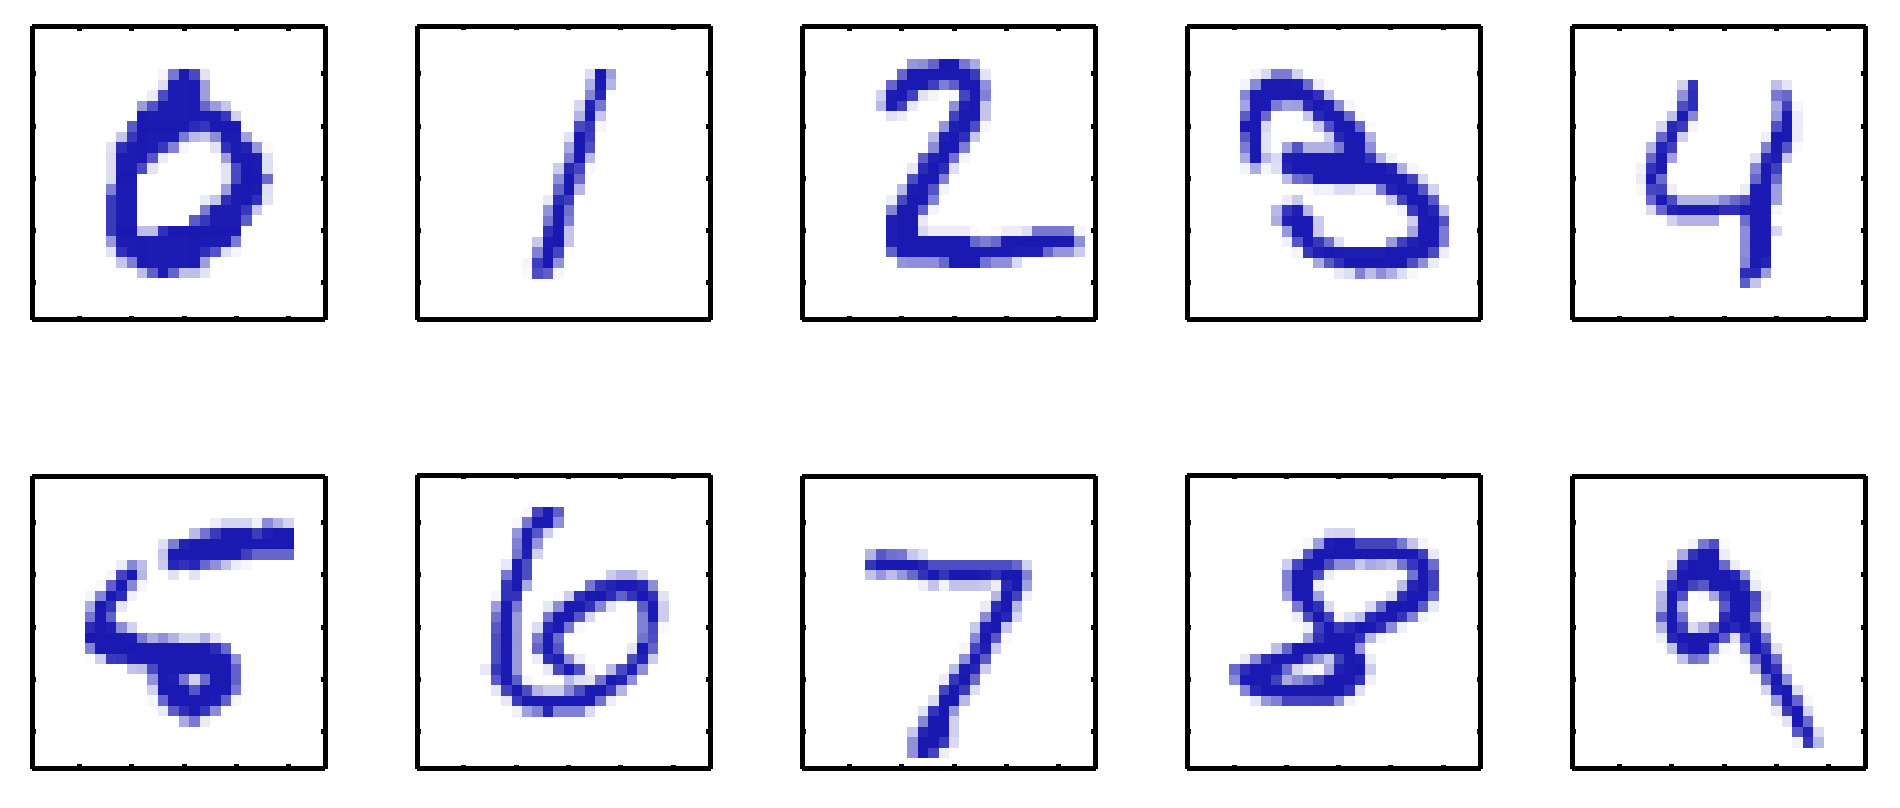
\includegraphics[scale=0.8]{Images/1-1.png}
		\captionsetup{font={small}}
		\caption{来自美国邮政编码的手写数字示例} 
		\label{fig:1-1}	
	\end{figure}
	\\
	\indent 通过机器学习,我们可以取得更好的结果。在机器学习方法中,我们会利用一个较大的训练集(training set)${\{ \textbf{x}_1,...,\textbf{x}_N\}}$来调节某个自适应模型的参数,训练集中包含有$N$个数字。训练集中的数字类别是已知的,一般要通过单独考察和手动标注。我们可以通过一个目标向量$\textbf{t}$来表示一个数字的类别,从而表征每个数字对应的特性。以向量形式表示类别的有效手段将在后文中进行论述。注意,对于每一个数字图像$\textbf{x}$,仅有一个这样的目标向量$\textbf{t}$。\\
	\indent 机器学习算法的运行结果可以表示为函数$\textbf{y}(\textbf{x})$,该函数将一个新的数字图像$\textbf{x}$作为输入并生成一个与目标向量形式相同的输出向量$\textbf{y}$。函数$\textbf{y}(\textbf{x})$的具体形式基于训练数据,确定于训练阶段,该阶段也被称为学习阶段。模型一旦完成训练,它就可以对测试集(test set)中新的数字图像进行分类。正确区分与训练实例不同的新实例的能力称为泛化(generalization)。在实际应用中,输入向量的多变性使得训练数据往往只能够覆盖到所有可能的输入变量中的一小部分,所以泛化是模式识别的核心目标之一。\\
	\indent 对于大部分的实际应用而言,初始的输入变量通常都是经过预处理的。我们将其变换到了新的向量空间,以期望在新的向量空间中,模式识别问题解决起来会变得容易一些。例如,在数字识别问题中,数字图像通常会经过变换和缩放,从而使每个数字都位于尺寸比较合适的方框中。这一做法大幅减少了每种数字的多变性,因为所有数字的位置和尺寸都变成相同的之后,随后的模式识别算法可以更加轻松地判断其类别。这种预处理步骤又会被称为特征提取(feature extraction)。注意,新的测试数据也必须经过和训练数据相同的预处理过程。\\
	\indent 为了提升计算的速度,也可能需要加入预处理的步骤。举例而言,如果我们的目标是在高分辨率的视频流中进行实时的人脸识别,计算机就必须在一秒钟内处理大量的像素,在复杂的模式识别算法中,用直接法表示像素,可能是算法根本无法计算的。所以,我们希望寻找出计算较快且具有较强区分度的特征,有效区分人脸与非人脸。这些特征就是接下来输入到模式识别算法的输入量。举例而言,我们可以评估矩形子区域上的图像灰度均值(Viola and Jones, 2004),这样的特征集合在快速人脸检测中非常有效。由于特征数量小于像素数量,所以这样的预处理是降维的一种形式。在预处理的过程中务必要小心,因为在此过程中通常会有信息被丢弃,而如果丢弃的信息对问题的解决具有重要的作用,那么整个系统的准确性都会大打折扣。\\
	\indent 如果训练数据中包含了输入向量及其对应的目标向量,那么这样的应用就称为监督学习(supervised learning)问题。类似于上文中数字识别案例的情况称为分类(classification)问题,分类问题的目标是对每个输入向量分配一个离散的类别,且类别的数量是有限的。如果希望得到的输出是由一个或多个连续变量组成的,那么就变成了一个回归(regression)问题。在化学生产过程中,以反应物浓度、温度和压力为输入,预测产量的问题就是回归问题的一个案例。\\
	\indent 除此之外还有一些其他形式的模式识别问题,这些问题中的训练数据仅仅是一个输入向量$\textbf{x}$的集合,没有任何对应的目标值。在这样的无监督学习(unsupervised learning)问题中,我们的目标可能是发现数据中相似实例的分组情况,这样的问题被称为聚类(clustering),或者是确定输入空间中数据的分布情况,这样的问题被称为密度估计(density estimation),亦或是将数据从高维空间投影到二维或三维中,进行数据的可视化(visualization)。\\
	\indent 最后,强化学习(reinforcement learning, Sutton and Barto, 1998)的目的是,在给定的情况下寻找到合适的行为,从而使获得的奖励达到最大。与监督学习相比,强化学习算法不会被告知哪些是最优的输出,而是必须在不断的实验试错中将最优输出分析出来。通常而言,在学习算法与环境的不断交互下,会产生一个状态和行为的序列。在多数情况下,当前的行为不仅仅会影响当前的奖励,还有可能在后续的任何时间节点对获得的奖励造成影响。举例而言,通过使用适当的强化学习技术,一个神经网络可以通过学习,使自己玩十五子棋游戏的能力达到很高的水平(Tesauro, 1994)。在这个问题中,神经网络将棋盘的当前情况和骰子投掷的结果一同作为输入,以具有威力的移动作为网络的输出。这是通过让神经网络与自己的复制品进行游戏来完成的,可能需要经历一百万次的游戏。一个主要的挑战是,十五子棋游戏可能包含很多的步骤,但只有在游戏结束时,才能以胜利或失败的形式收获奖励。所以,即使是好棋和坏棋并存的情况,奖励也必须归功于所有指向最终结果的步骤。这是信用分配问题的案例之一。强化学习的一般特征之一,是进行探索(exploration)和开发(exploitation)之间的制衡。在探索中,系统要尝试新的行为并验证其有效性;在开发中,系统要利用已知的行为,来获得更高的奖励。过多地关注探索或开发都会导致不良的结果。强化学习仍然是机器学习研究中的一个活跃领域,但本书中不包含对于强化学习的详细讨论。\\
	\indent 尽管每一个问题都需要各自的工具和技术,但对于所有的问题,解决它们的许多关键思想是相同的。本章的主要目标之一,就是以相对不太正式的方式,介绍一些很重要的概念,并利用一些简单的例子来解释它们。在这本书的后续内容中我们将看到,在现实世界中的模式识别应用里,相同的思想会再次出现在更加复杂的模型中。本章还提供了本书中即将使用的三个重要工具的介绍,即概率论、决策论和信息论。尽管听起来可能很吓人,但实际上它们很直观,而且如果希望使用机器学习技术在实际应用中得到最佳的效果,那么对它们有一个清晰的理解是不可或缺的。}

	\section{实例:多项式曲线拟合}
	\noindent{\color{red} \rule[10pt]{\textwidth}{0.1em}}
	\textnormal{
	\indent 我们从一个简单的回归问题开始,而且我们将在本章节中一直以这个问题为案例,介绍一系列关键的概念。假设我们对实值输入变量$x$进行观测,并希望利用观测结果来预测实值目标变量$t$。对于这样的目的,一个比较好的方法是研究一个基于人为生成数据的人造案例,因为这样我们可以完全获悉数据的详细生成过程,就可以与任何学习模型进行比较了。该案例中的数据是基于函数$\sin (2\pi x)$生成的,数据中的目标变量带有随机噪声,相关的内容可详见于附录A。\\
	\indent 假设我们现在有一个给定的训练集,其中包含有$N$个对$x$的观测,记作$\boldsymbol{\mathsf{x}} \equiv (x_1,...,x_N)^\mathrm{T}$, 同时有与之对应的目标变量$t$,记作$\boldsymbol{\mathsf{t}} \equiv (t_1,...,t_N)^\mathrm{T}$。图1.2展示了一个包含有$N=10$个数据点的训练集。图1.2中的输入数据集合$\boldsymbol{\mathsf{x}}$通过在[0,1]之间随机等可能地选取$x_n$来生成,其中$n=1,...,N$;而对于目标数据集合$\boldsymbol{\mathsf{t}}$,首先计算对应的函数值$\sin {(2 \pi x)}$,然后对每一个点加上一个较小且服从高斯分布的随机噪声,从而得到$x_n$对应的值$t_n$。高斯分布将在第1.2.4节中进行详细的介绍。通过这样的方式生成数据,可以获取很多真实数据集中的属性。换句话说,就是个别观测受到随机噪声干扰的数据中包含的潜在规律,而这些潜在规律就是我们希望学习的。随机噪声可能是由随机过程产生的,例如放射性衰变,但更多的情况下是由于存在缺乏观测的噪声源而形成的。
	\begin{figure}[ht]
		\centering
		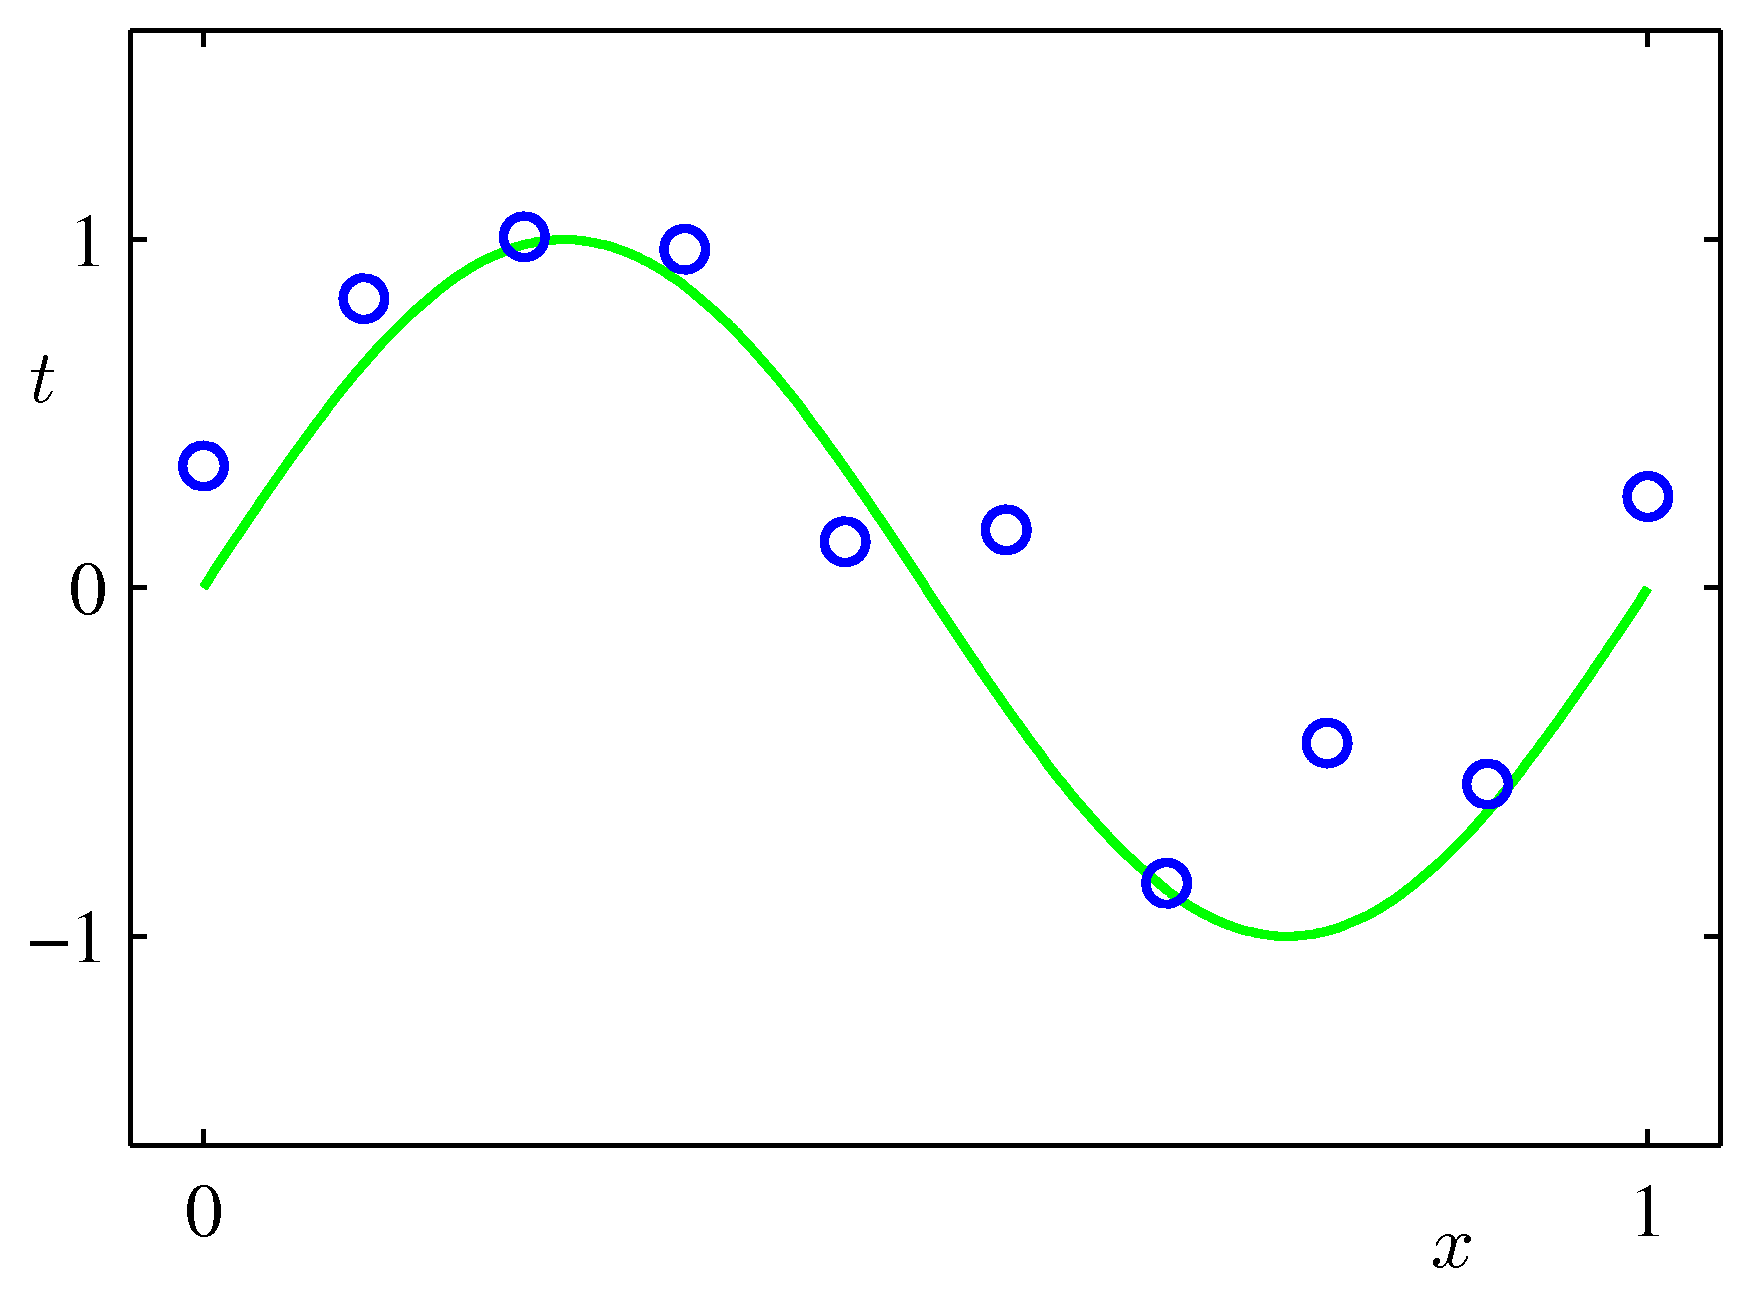
\includegraphics[scale=0.8]{Images/1-2.png}
		\captionsetup{font={small}}
		\caption{一个包含了$N=10$个点的训练集的图像,如图中蓝色圆圈所示,每个点都包括了输入变量$x$的观测值及其对应的目标变量值$t$。绿色的曲线表示用于生成数据的函数$\sin (2 \pi x)$。我们的目标是在绿色曲线未知的情况下,对于新的$x$值,预测其对应的$t$值。} 
		\label{fig:1-2}	
	\end{figure}
	\\
	\indent 我们的目标是对训练集加以利用,从而对新的输入变量$\hat{x}$进行其对应目标变量$\hat{t}$的预测。正如我们接下来将看到的一样,这个过程隐式地包含了发现数据中隐含的函数$\sin (2 \pi x)$。这似乎是一个困难的事情,因为我们需要利用一个有限的数据集将这个隐含的函数归纳出来。而且,我们得到的观测数据是受到噪声干扰的,于是对于给定的$\hat x$,估计出来的$\hat t$是具有不确定性的。为了研究这种不确定性,第1.2节中的概率论提供了一个可以精确、定量表示不确定性的框架;同时,第1.5节中的决策论使得我们可以利用不确定性的概率表示进行适当标准下的最优预测。\\
	\indent 不过现在我们也将不太正式地继续分析下去,研究一个基于曲线拟合的简单方法。特别地,我们将使用如下形式的多项式函数进行数据拟合:
	\begin{equation}
		y(x,\mathbf{w})= w_0 + w_1 x + w_2 x^2 + ... + w_M x^M = \sum_{j=0}^M w_j x^j
	\end{equation}
	其中$M$是多项式的阶(order),$x^j$表示变量$x$的$j$次方。多项式系数$w_0,...,w_m$可以集合在一起,用向量$\mathbf{w}$表示。需要注意的是,尽管多项式函数$y(x,\mathbf{w})$是一个关于$x$的非线性函数,但它也是一个关于系数$\mathbf{w}$的线性函数。关于未知参数的线性函数,比如这个多项式函数,被称为线性模型(linear models)。线性模型具有很多重要的性质,将在第3章和第4章中详细介绍。\\
	\indent 我们可以根据训练数据调整多项式函数,从而确定这些系数的值。这项任务可以通过误差函数(error function)的最小化来完成。误差函数衡量的是对于任意的$\mathbf{w}$,函数值$y(x,\mathbf{w})$与训练集数据点之间的差距。一种广泛应用而且比较简单的误差函数是求取每一个数据点$x_n$上的预测值$y(x_n,\mathbf{w})$与对应的目标变量$t_n$差值的平方和,于是我们需要将如下函数进行最小化:
	\begin{equation}
	E(\mathbf{w}) = \frac{1}{2} \sum_{n=1}^N \{y(x_n,\mathbf{w}) - t_n\}^2
	\end{equation}
	其中的系数$1/2$是为了接下来计算的方便添加的。选择这样的误差函数的理由也将在本章节稍后的内容中进行介绍。现在我们只需注意到它是一个非负函数,当且仅当所有训练数据点都在函数$y(x,\mathbf{w})$上时,误差函数的值为0。平方和误差函数的几何解释如图1.3所示。
	\begin{figure}[ht]
		\centering
		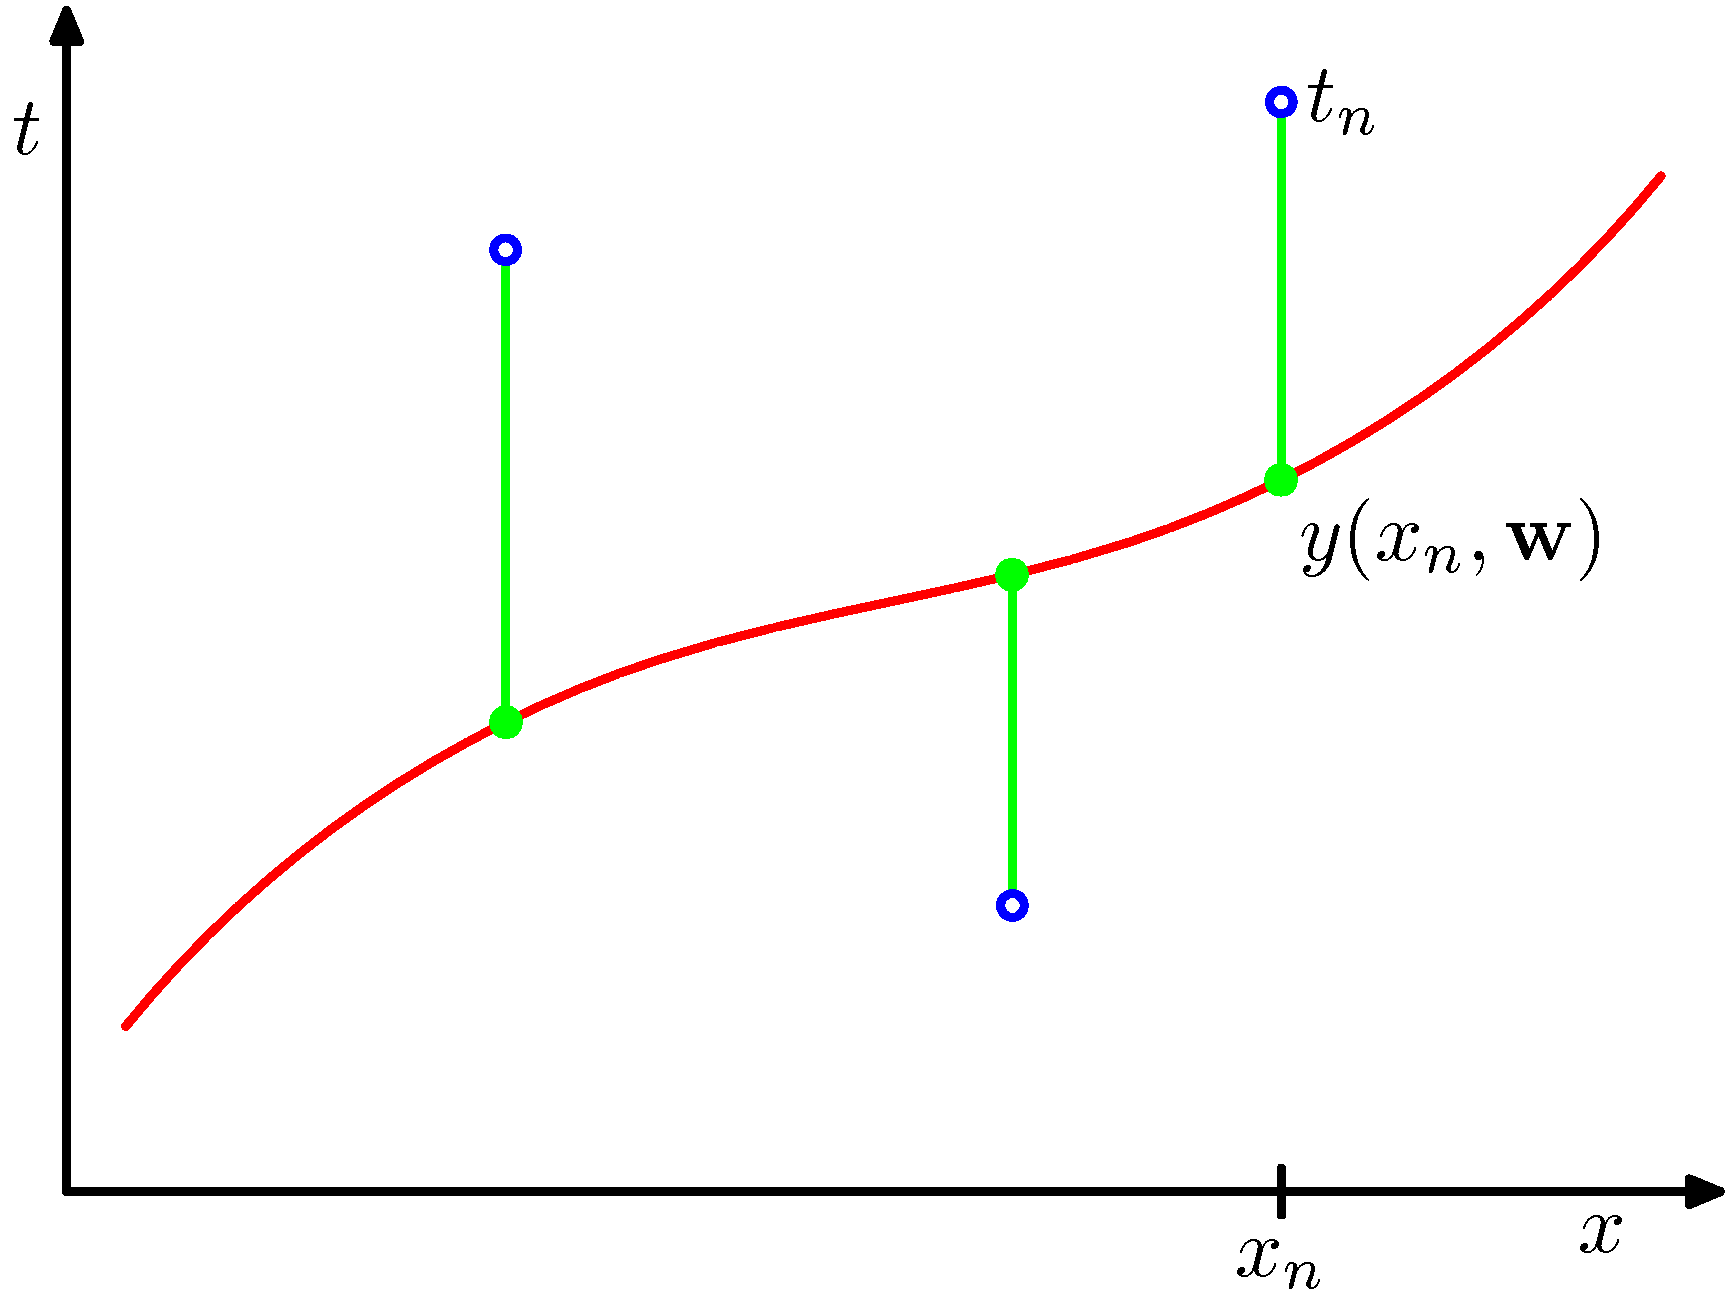
\includegraphics[scale=0.8]{Images/1-3.png}
		\captionsetup{font={small}}
		\caption{误差函数(1.2)对应每个数据点与函数$y(x, \mathbf{w})$之间相差距离(绿色垂直线)的平方和(的一半)。} 
		\label{fig:1-3}	
	\end{figure}
	\\
	\indent 我们可以通过选择使得$E(\mathbf{w})$尽可能小的$\mathbf{w}$来解决这个曲线拟合问题。由于误差函数对于系数$\mathbf{w}$是一个二次函数,所以误差函数的导数对于$\mathbf{w}$是线性的,所以误差函数最小化的结果是唯一的,可以求取其解析解$\mathbf{w^\star}$。最终得到的结果为多项式函数$y(x,\mathbf{w^\star})$。\color{red} \textbf{——习题 1.1}\\
	\color{black}
	\indent 还有一个问题是选择多项式的阶数$M$。它的背后是一个重要的问题——模型对比(model comparison,或称为模型选择,model selection)。在图1.4中,我们展示了在阶数$M=0,1,3$和$9$时,对于图1.2所示的数据集的拟合结果。
	\begin{figure}[ht]
		\begin{minipage}[t]{0.5\linewidth}
		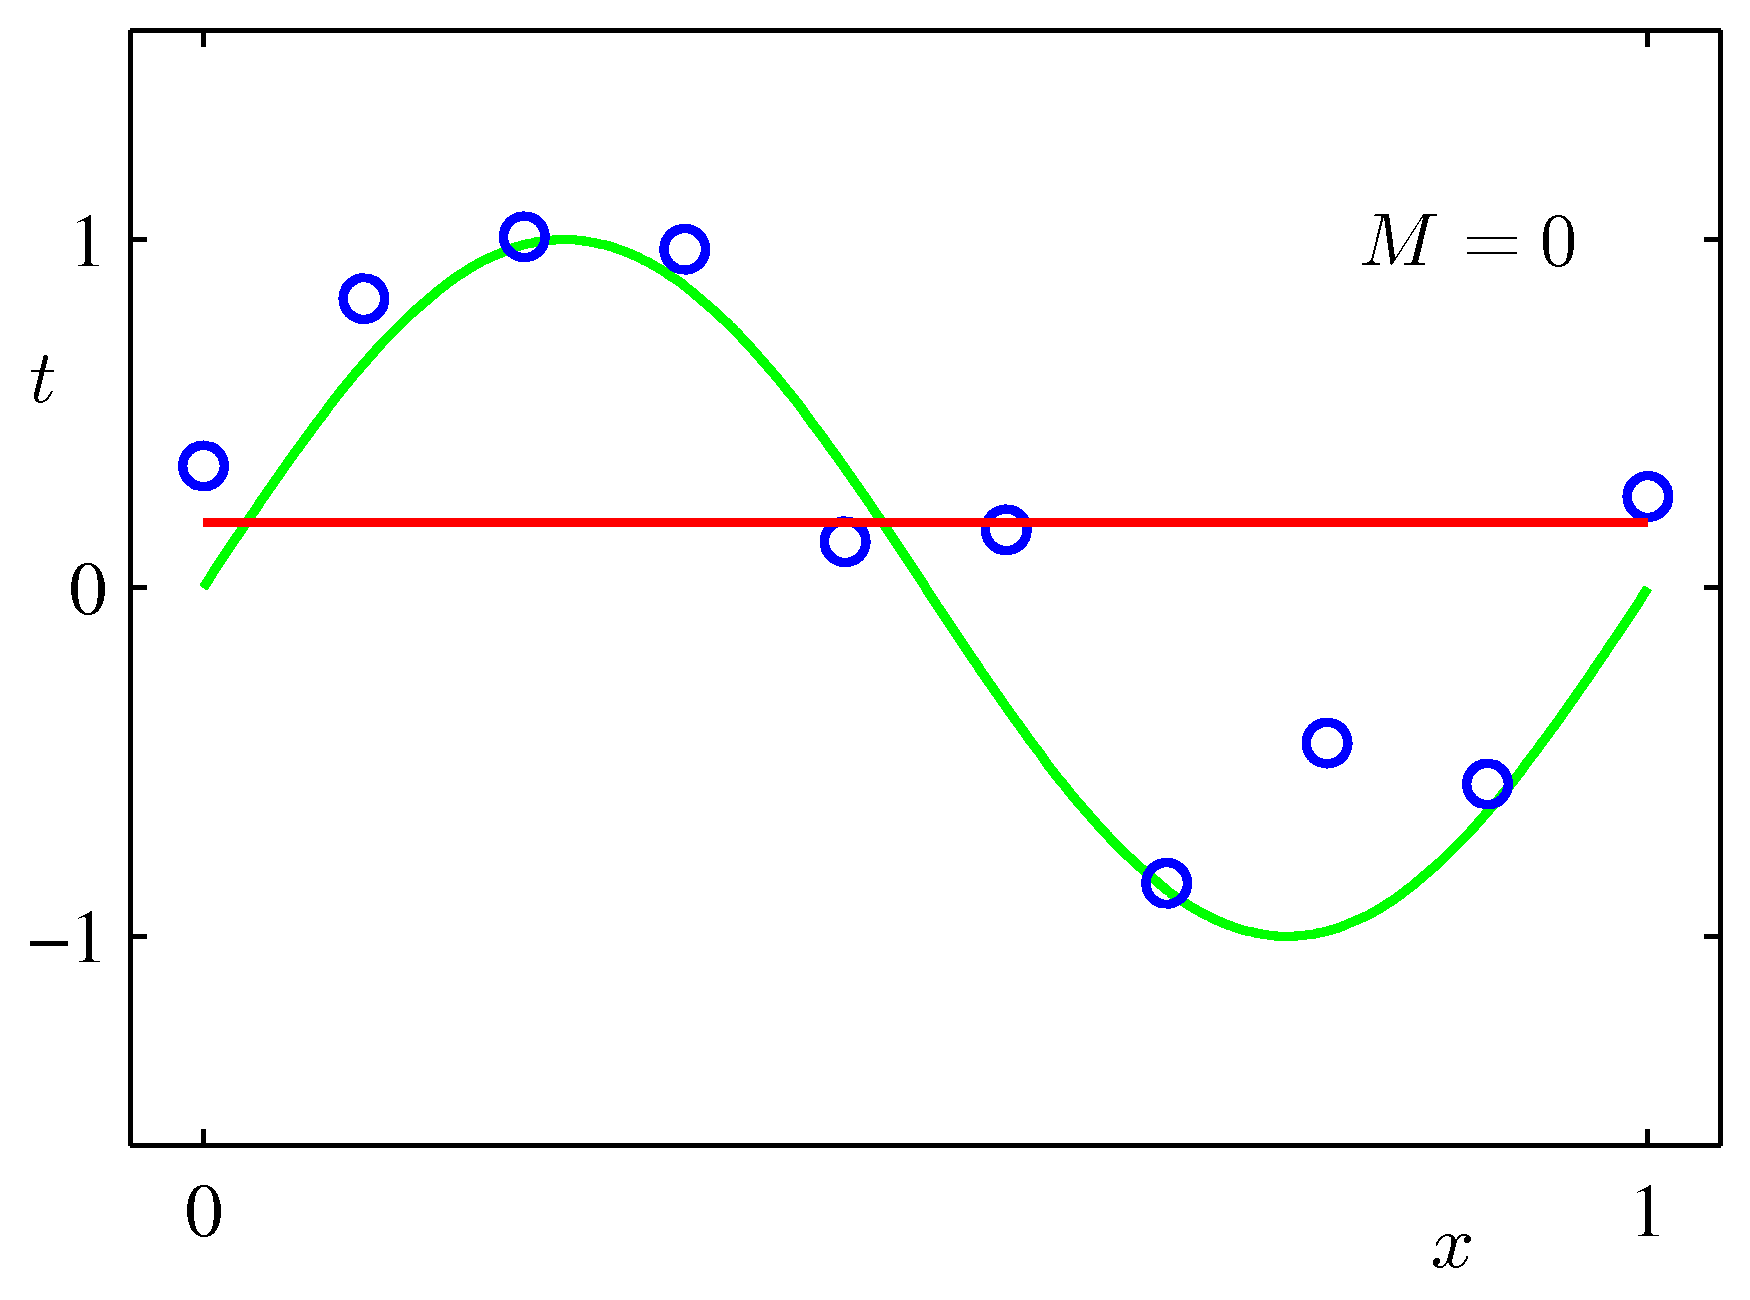
\includegraphics[scale=0.8]{Images/1-4a.png}
		\label{fig:1-4a}
		\end{minipage}
		\begin{minipage}[t]{0.5\linewidth}
		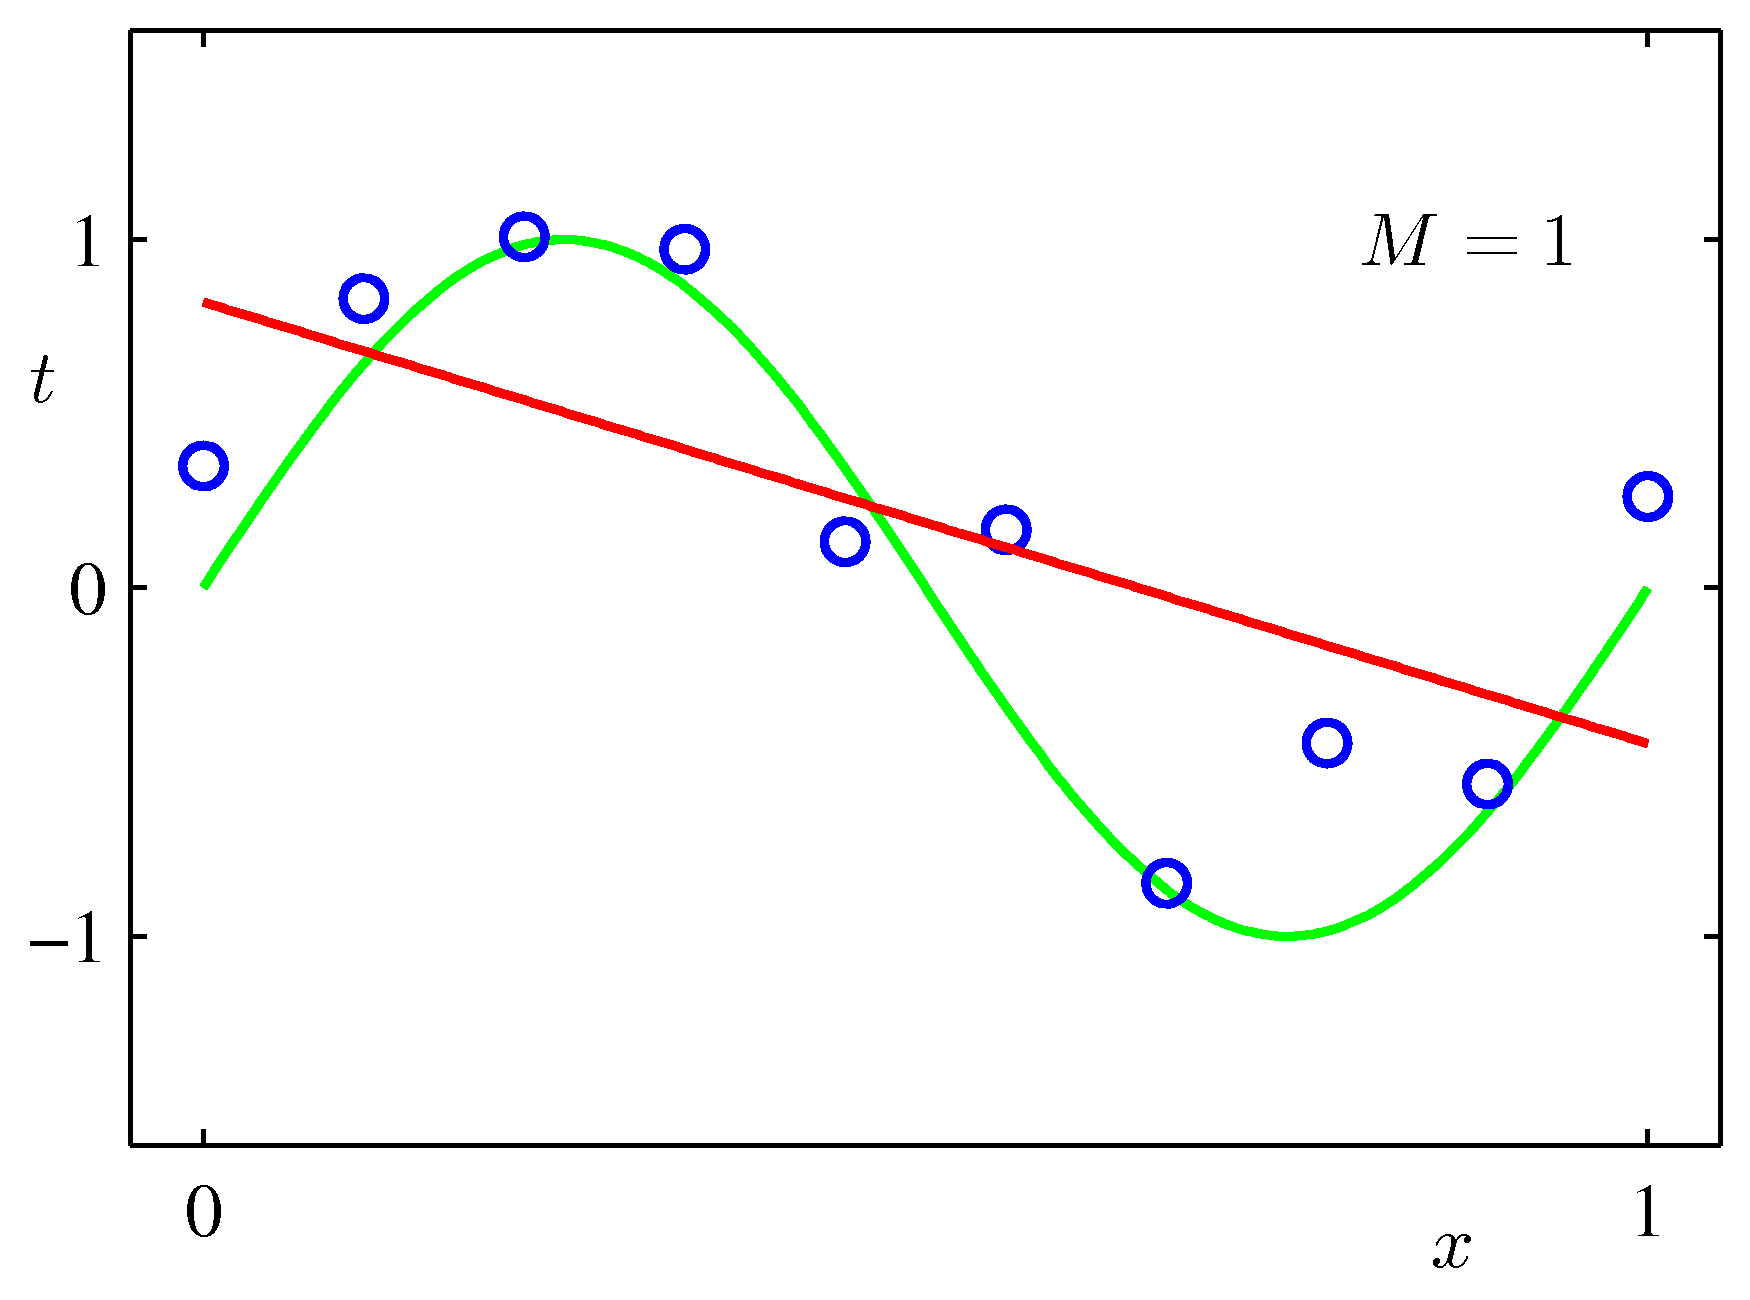
\includegraphics[scale=0.8]{Images/1-4b.png}
		\label{fig:1-4b}
		\end{minipage} \\
		\begin{minipage}[t]{0.5\linewidth}
		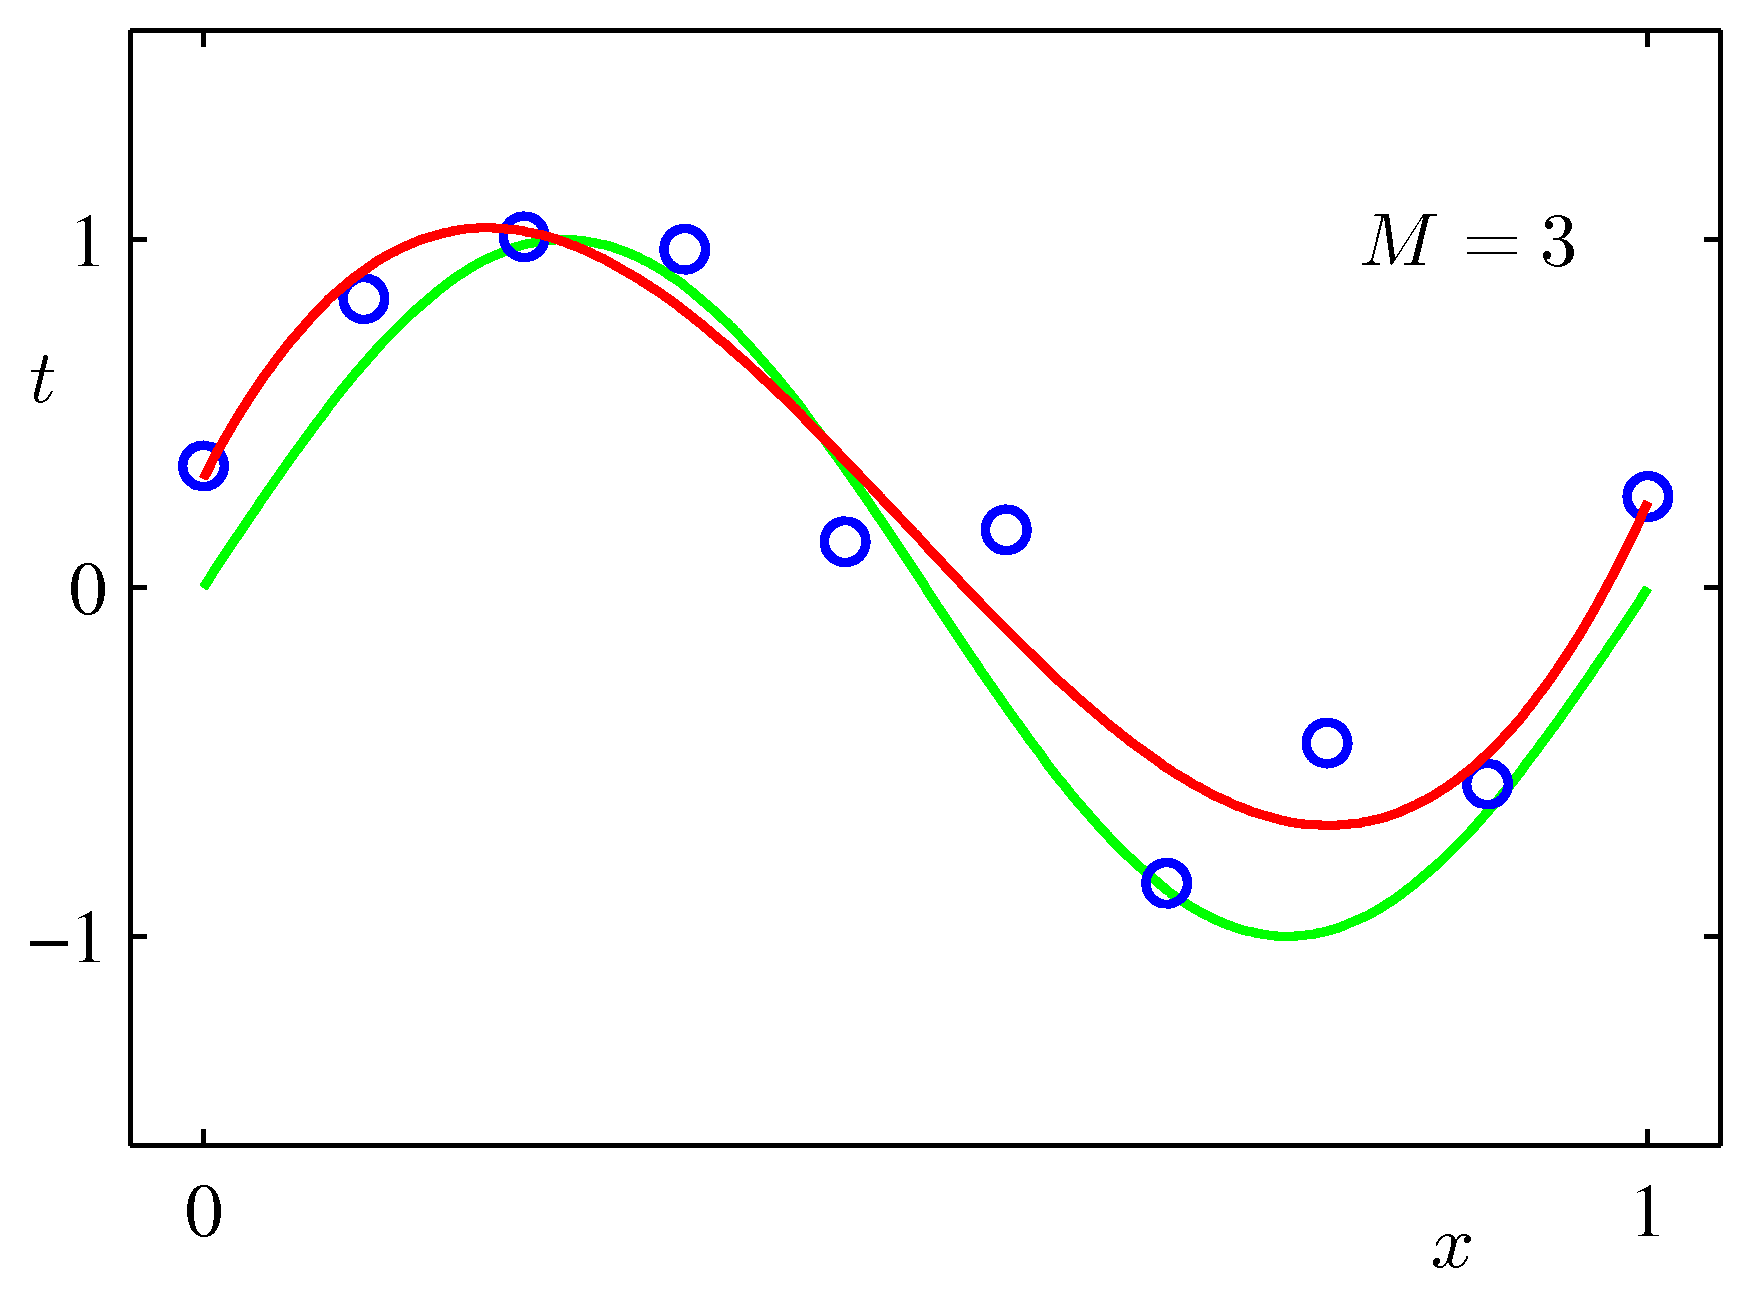
\includegraphics[scale=0.8]{Images/1-4c.png}
		\label{fig:1-4c}
		\end{minipage}
		\begin{minipage}[t]{0.5\linewidth}
		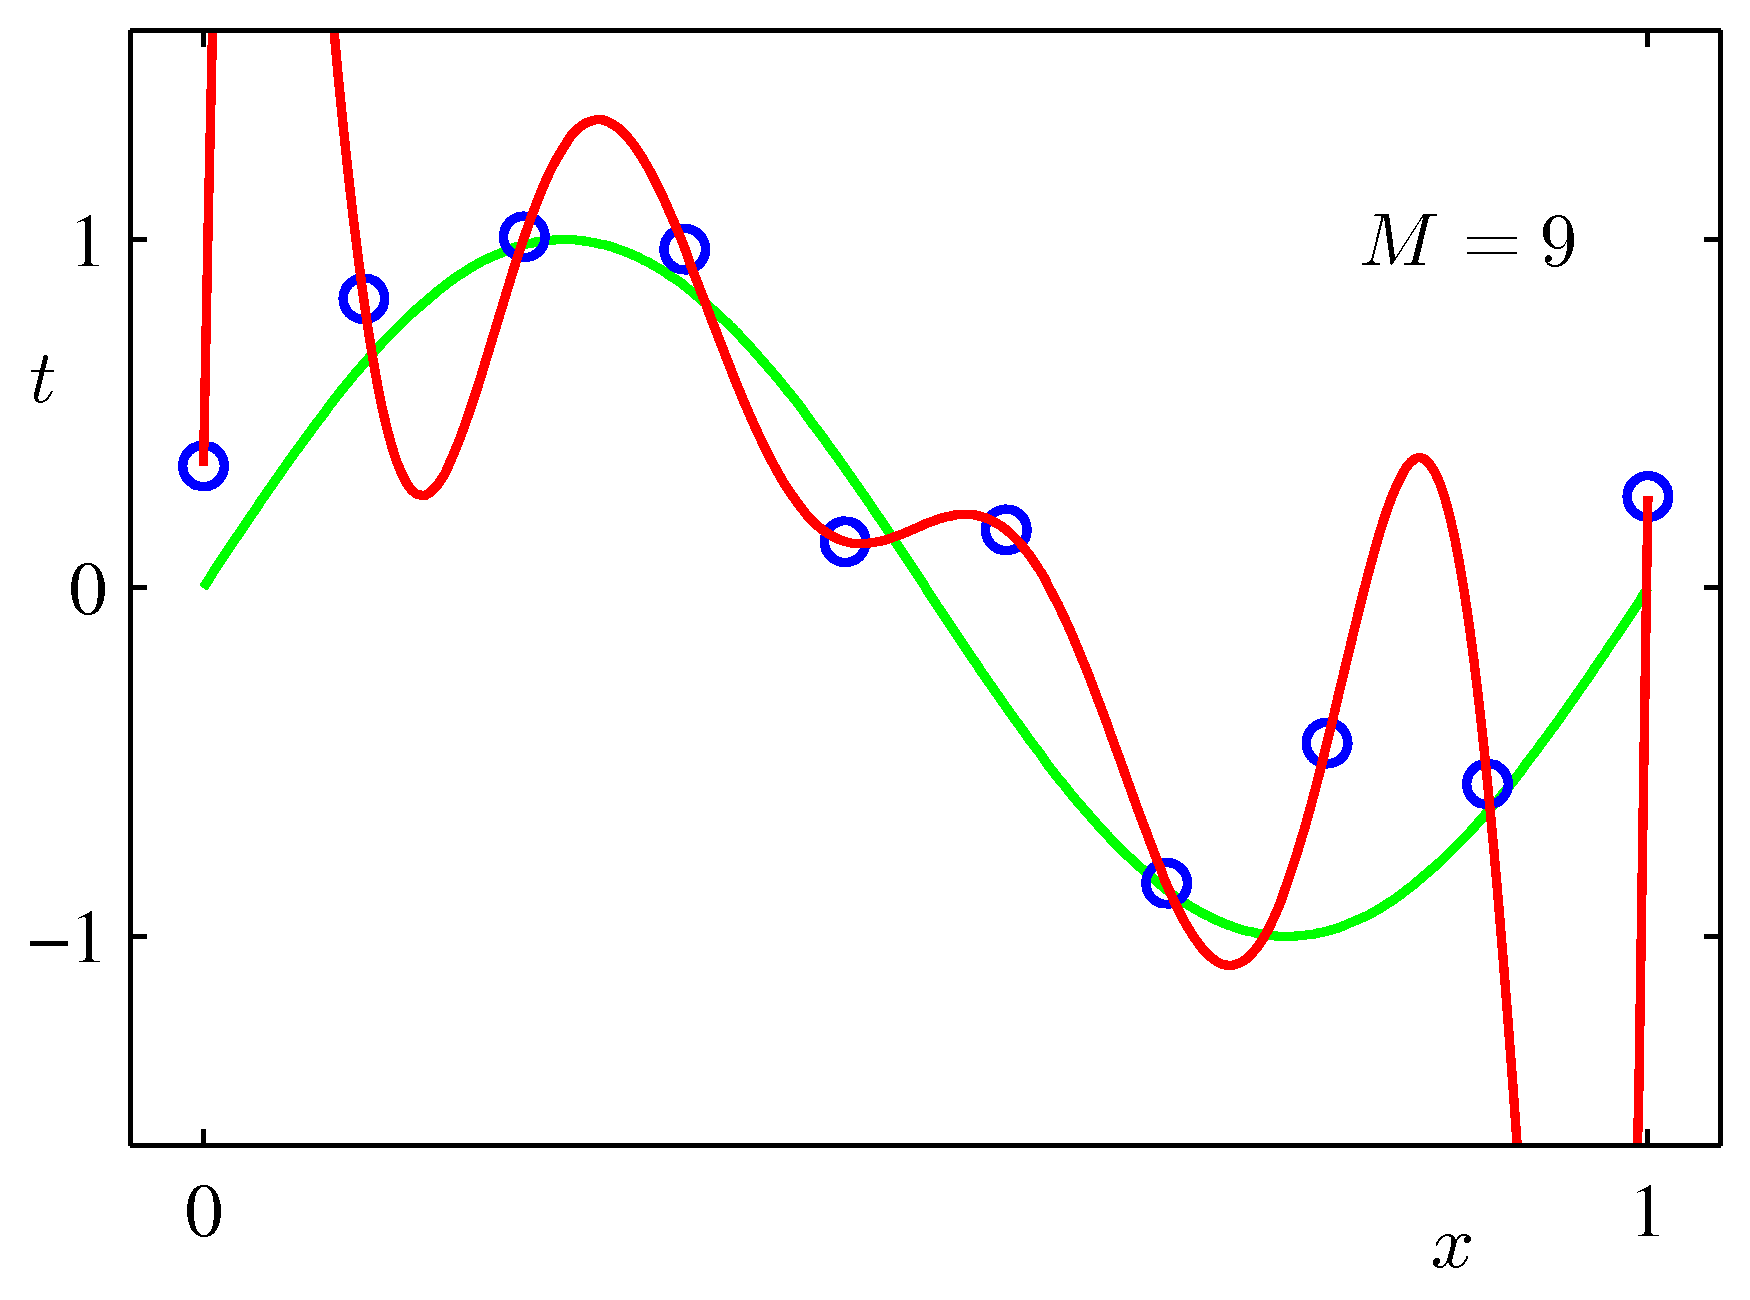
\includegraphics[scale=0.8]{Images/1-4d.png}
		\label{fig:1-4d}
		\end{minipage}
		\captionsetup{font={small}}
		\caption{在$M$变化时的拟合图1.2所示数据的多项式图像(红色曲线)。}
	\end{figure}
	\\
	\indent 我们注意到,在函数为常数($M=0$)和一阶函数($M=1$)时,对于数据的拟合效果相当差,几乎没法表达函数$\sin (2 \pi x)$。三阶函数($M=3$)看起来是本例中对函数$\sin (2 \pi x)$最佳的拟合。当我们再提高多项式的阶数,到了很高的阶数($M=9$)时,我们得到了一个特别好的拟合结果。其实在这种情况下,所有数据点都在多项式函数上,所以$E(\mathbf{w^\star})=0$。然而,这样的拟合结果振荡得很厉害,而且对函数$\sin (2 \pi x)$的表达同样很差。这样的情况我们称之为过拟合(over-fitting)。\\
	\indent 前面我们已经提到了,我们的目标是让模型具有较好的泛化能力,从而对新数据也有准确的预测能力。我们可以利用一个独立的测试集来获得$M$对泛化性能影响程度的定量分析。该测试集中有100个数据点,这些数据点的生成方式与训练集完全相同,但目标值中包含的随机噪声有所不同。对任意的$M$,我们可以根据(1.2)估计$E(\mathbf{w^\star})$关于训练数据的残差值,同样地我们也可以估计$E(\mathbf{w^\star})$关于测试数据的残差。有时使用均方根误差(RMS error,root-mean-square error)更加方便,由以下公式定义:
	\begin{equation}
	E_{\textnormal{RMS}}=\sqrt{2E(\mathbf{w^\star})/N}
	\end{equation}
	其中除以$N$的做法是为了对于不同大小的数据集进行公平的分析,而平方根可以保证$E_{\textnormal{RMS}}$使用与目标变量$t$相同的比例(和单位)进行误差的衡量。在$M$取不同的值时,训练集和测试集的RMS误差图如图1.5所示。测试集的误差刻画了对于新的数据$x$产生的预测值$t$的准确程度。从图1.5可知,较小的$M$值会导致较大的测试集误差,这可以归因于这时的多项式不够灵活,以致于难以准确刻画函数$\sin (2 \pi x)$的振荡情况。在$3 \leqslant M \leqslant 8$范围内的$M$值可以使测试集误差变得很小,它们对函数$\sin (2 \pi x)$也形成了比较合理的近似表达,比如如图1.4所示的$M=3$的情况。\\
	\indent 当$M=9$时,似乎是达到了我们最期望的情况,训练集误差变成了$0$,因为此时的多项式包含了10个自由度,对应于10个系数:$w_0,...,w_9$,所以可以针对训练集中的10个数据点进行精确的调整。然而,测试集的误差却变得特别大,正如图1.4中所示的那样,对应的函数$y(x,\mathbf{w^\star})$表现出了强烈的振荡。
	\begin{figure}[H]
		\centering
		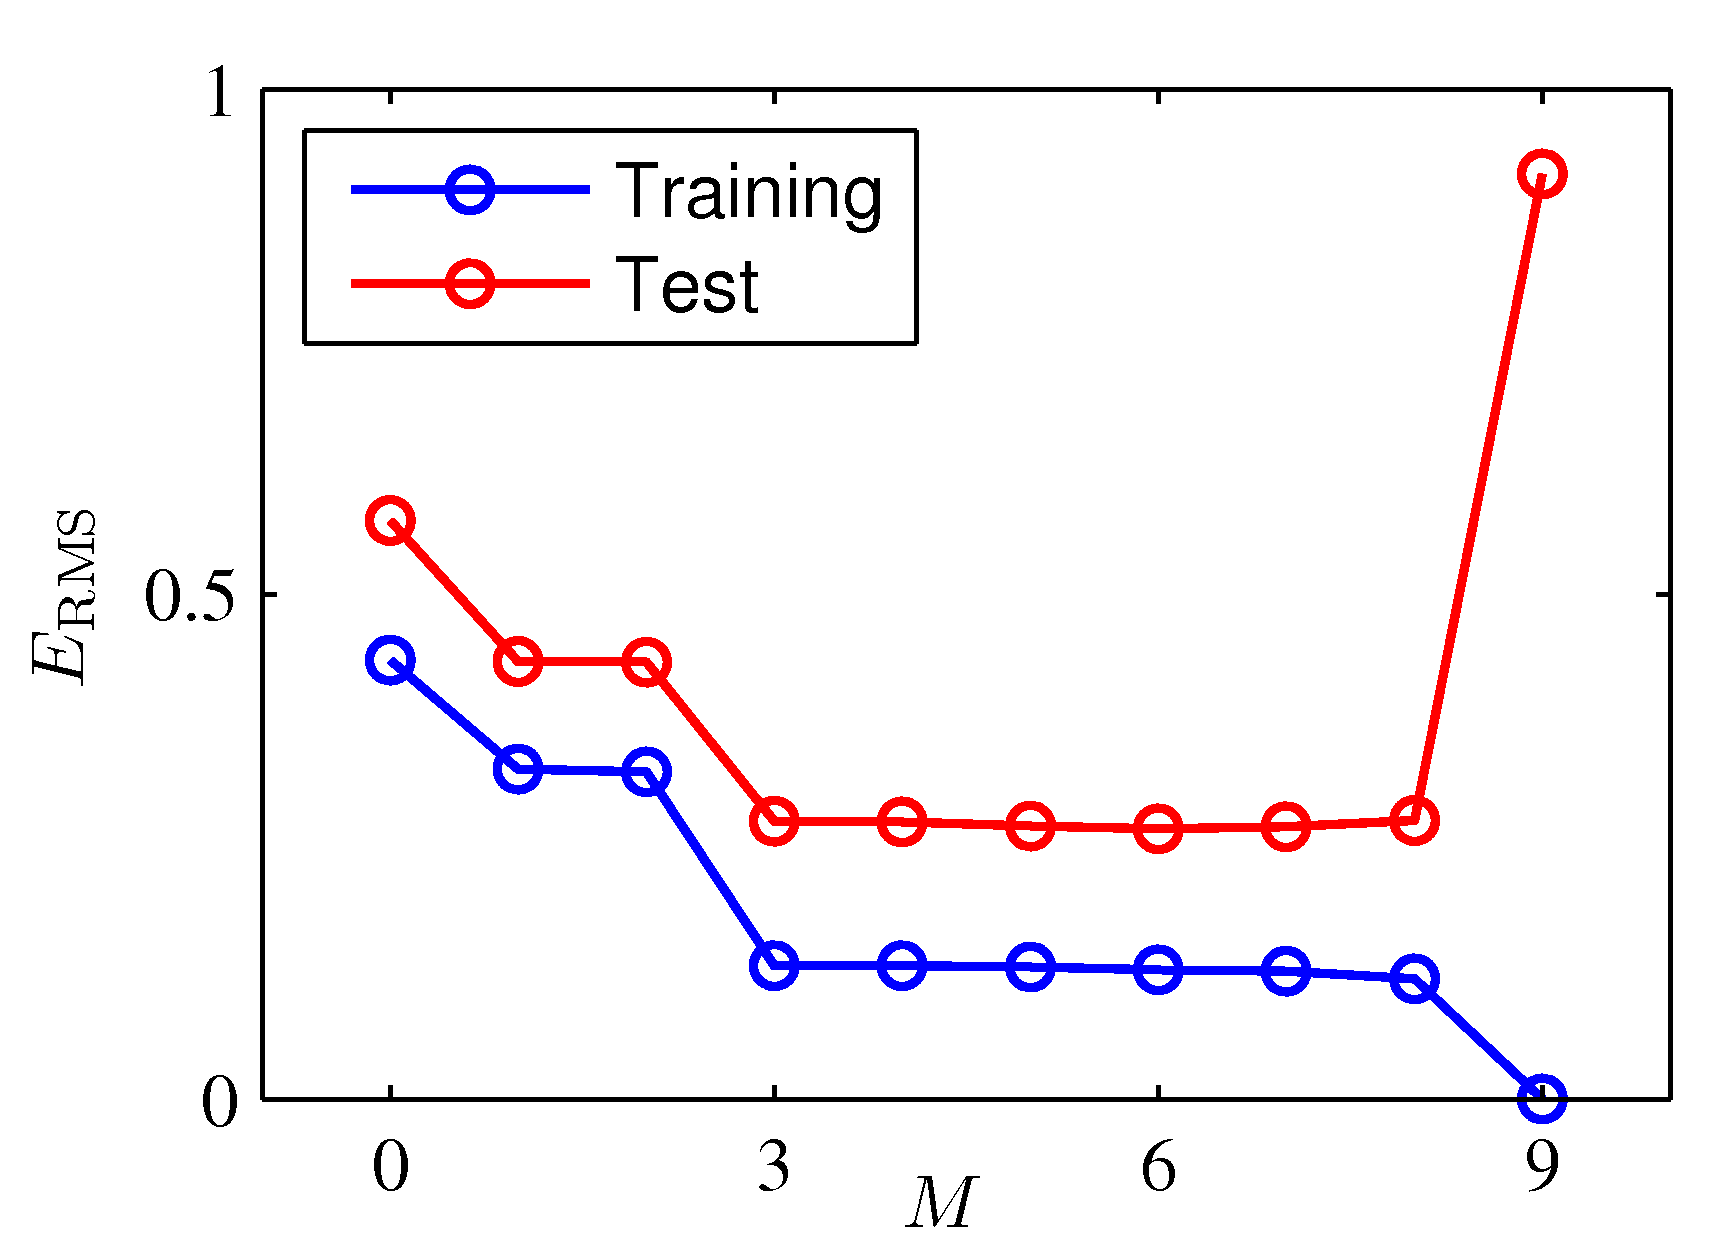
\includegraphics[scale=0.8]{Images/1-5.png}
		\captionsetup{font={small}}
		\caption{在不同的$M$值下,在训练集和独立测试集上根据(1.3)计算的均方根误差图像。} 
		\label{fig:1-5}	
	\end{figure}
	\indent 这看起来似乎有点自相矛盾,因为某个阶数一定的多项式应该包含了比它低阶的多项式,因为低阶多项式是高阶多项式的一种特殊情况。$M=9$的多项式至少应该取得与$M=3$的情况比较相似的结果。而且我们可以假设,对于新数据最优的预测函数为$\sin (2 \pi x)$(稍后我们会看到确实是这样的),因为数据就是从这个函数生成的。我们知道函数$\sin (2 \pi x)$的幂级数展开包含了任意阶数的项,随着$M$的增长,我们应该得到更好的近似结果。\\
	\indent 我们可以通过研究不同阶数的多项式中系数$\mathbf{w^\star}$的值来得到更加深刻的分析,如表1.1所示。可以发现,随着$M$的增大,系数通常也会随之变大。特别地,在$M=9$时,系数需要取到相当大才能对数据形成精确的拟合,而且还是正值和负值都有。于是在每个数据点之间,尤其是接近整个训练集数据范围边缘的地方,函数发生了剧烈的振荡,如图1.4所示。直观而言,这种情况的出现是因为在$M$较大的时候多项式实在太过灵活,以至于在拟合的过程中把目标值中包含的随机噪声也考虑了进去。	\\
	\indent 另外还有一个比较有意思的事情,在数据集规模发生变化时,模型的性能也会随之变化,如图1.6所示。我们可以看到,对于给定的模型复杂度,随着数据集规模的增大,过拟合问题变得越来越不严重。换句话说,数据集越大,就可以用越复杂的(也就是越灵活的)模型来进行数据拟合。一个比较粗略的启发是,数据集中数据点的数量应不小于模型中可调节参数数量的若干倍(比如5倍、10倍)。然而,我们即将在第3章中看到,参数的数量并不一定是模型复杂度最合适的度量。\\
	\indent 不过另外有件事让人相当不爽,那就是必须根据训练集的规模来限制模型中参数的数量。明明应该根据问题的复杂程度来确定模型的复杂度,这样才更加合理。我们将看到,使用最小二乘法寻找模型参数是最大似然(maximum likelihood,将在第1.2.5节中进行讨论)的一种特殊情形,而过拟合问题可以被理解成最大似然的一般
	\begin{table}
		\centering
		\begin{tabular}{c|rrrr}
			\ & $M=0$ & $M=1$ & $M=3$ & $M=9$ \\
			\hline
			$w_0^\star$ & 0.19 & 0.82 & 0.31 & 0.35\\
			$w_1^\star$ & \  & -1.27 & 7.99 & 232.37\\
			$w_2^\star$ & \  & \  & -25.43 & -5321.83\\
			$w_3^\star$ & \  & \  & 17.37 & 48568.31\\
			$w_4^\star$ & \  & \  & \  & -231639.30\\
			$w_5^\star$ & \  & \  & \  & 640042.26\\
			$w_6^\star$ & \  & \  & \  & -1061800.52\\
			$w_7^\star$ & \  & \  & \  & 1042400.18\\
			$w_8^\star$ & \  & \  & \  & -557682.99\\
			$w_9^\star$ & \  & \  & \  & 125201.43\\
		\end{tabular}
		\captionsetup{font={small}}
		\caption{不同阶数的多项式中的系数$\mathbf{w^\star}$。显而易见,随着阶数的增长,系数的绝对值也在飞速增长。}
	\end{table}
	\begin{figure}[ht]
		\begin{minipage}[t]{0.5\linewidth}
		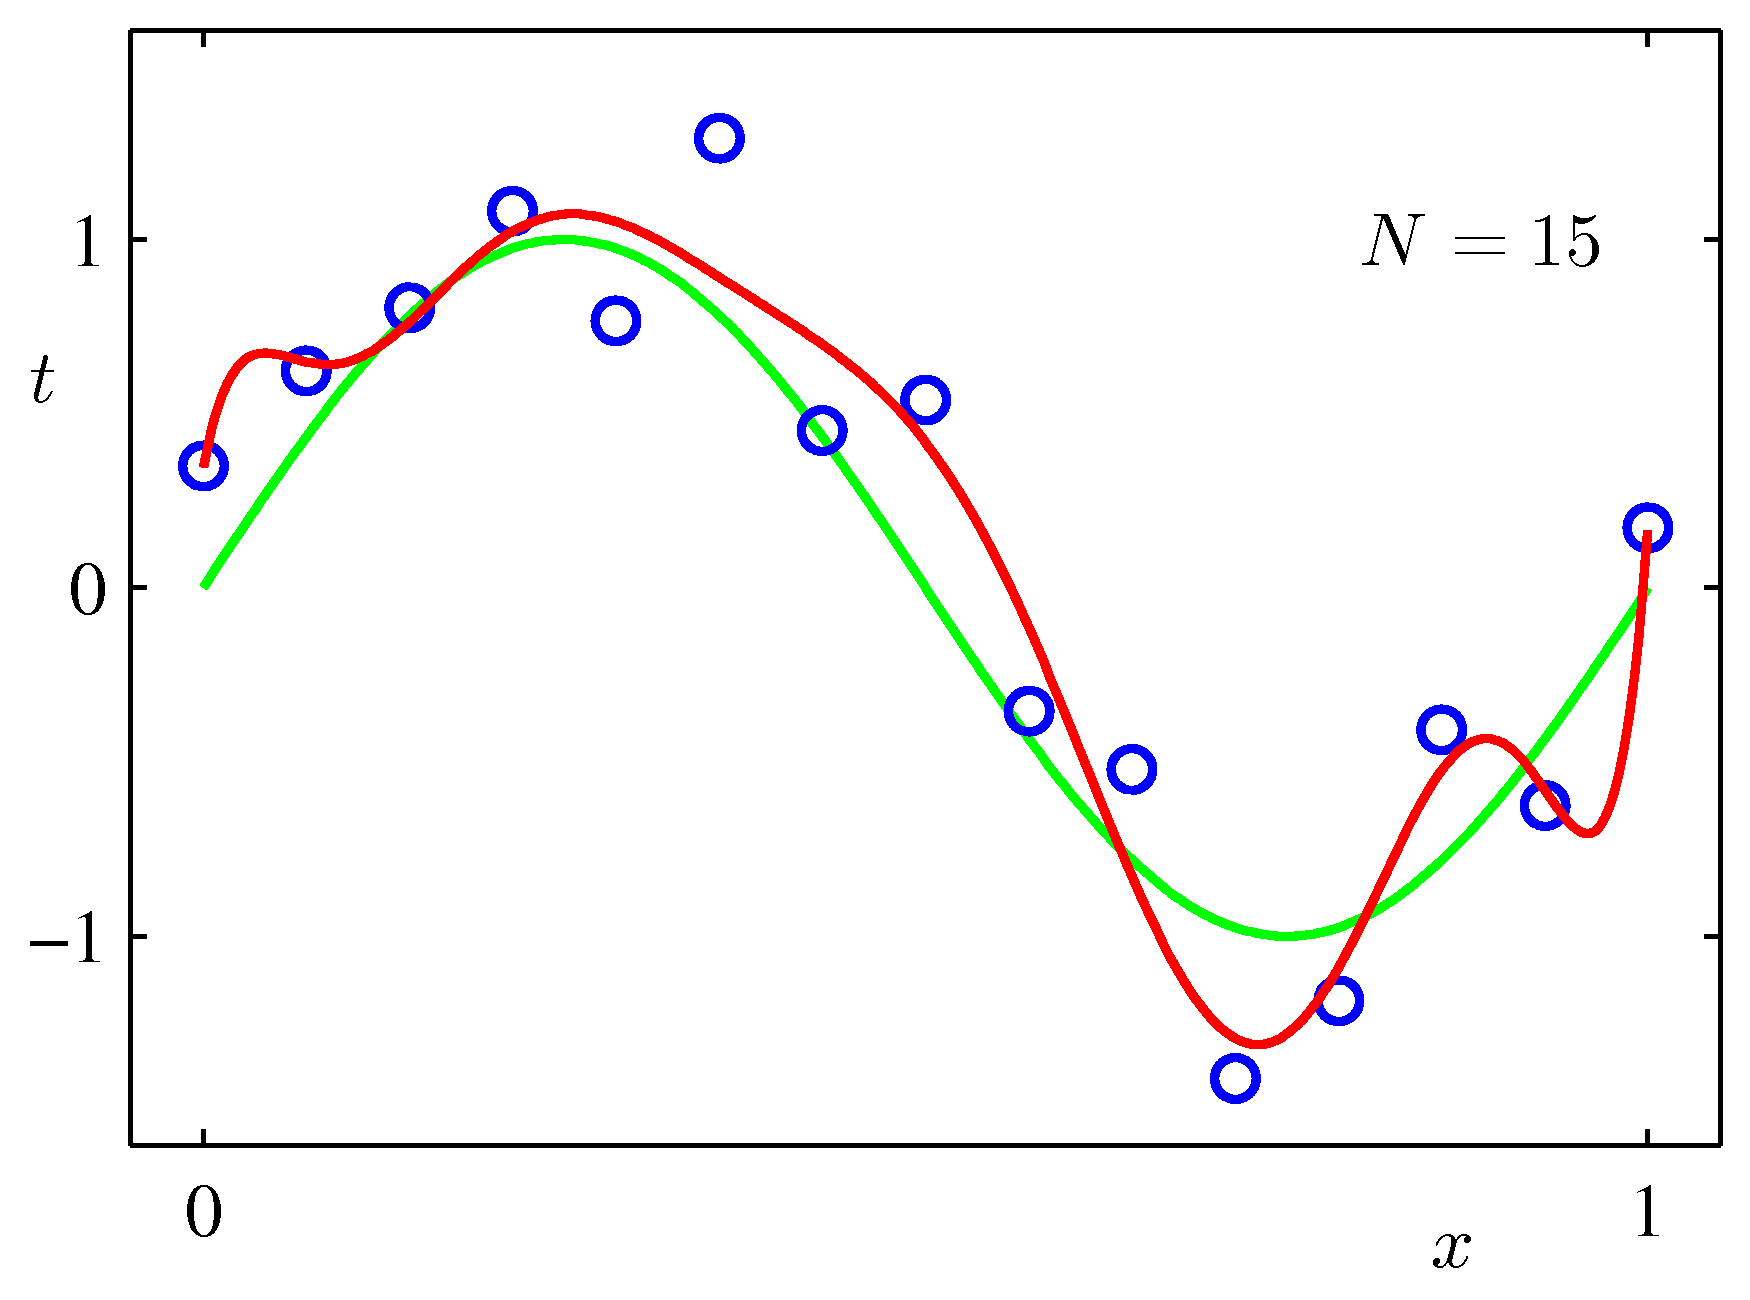
\includegraphics[scale=0.8]{Images/1-6a.png}
		\label{fig:1-6a}
		\end{minipage}
		\begin{minipage}[t]{0.5\linewidth}
		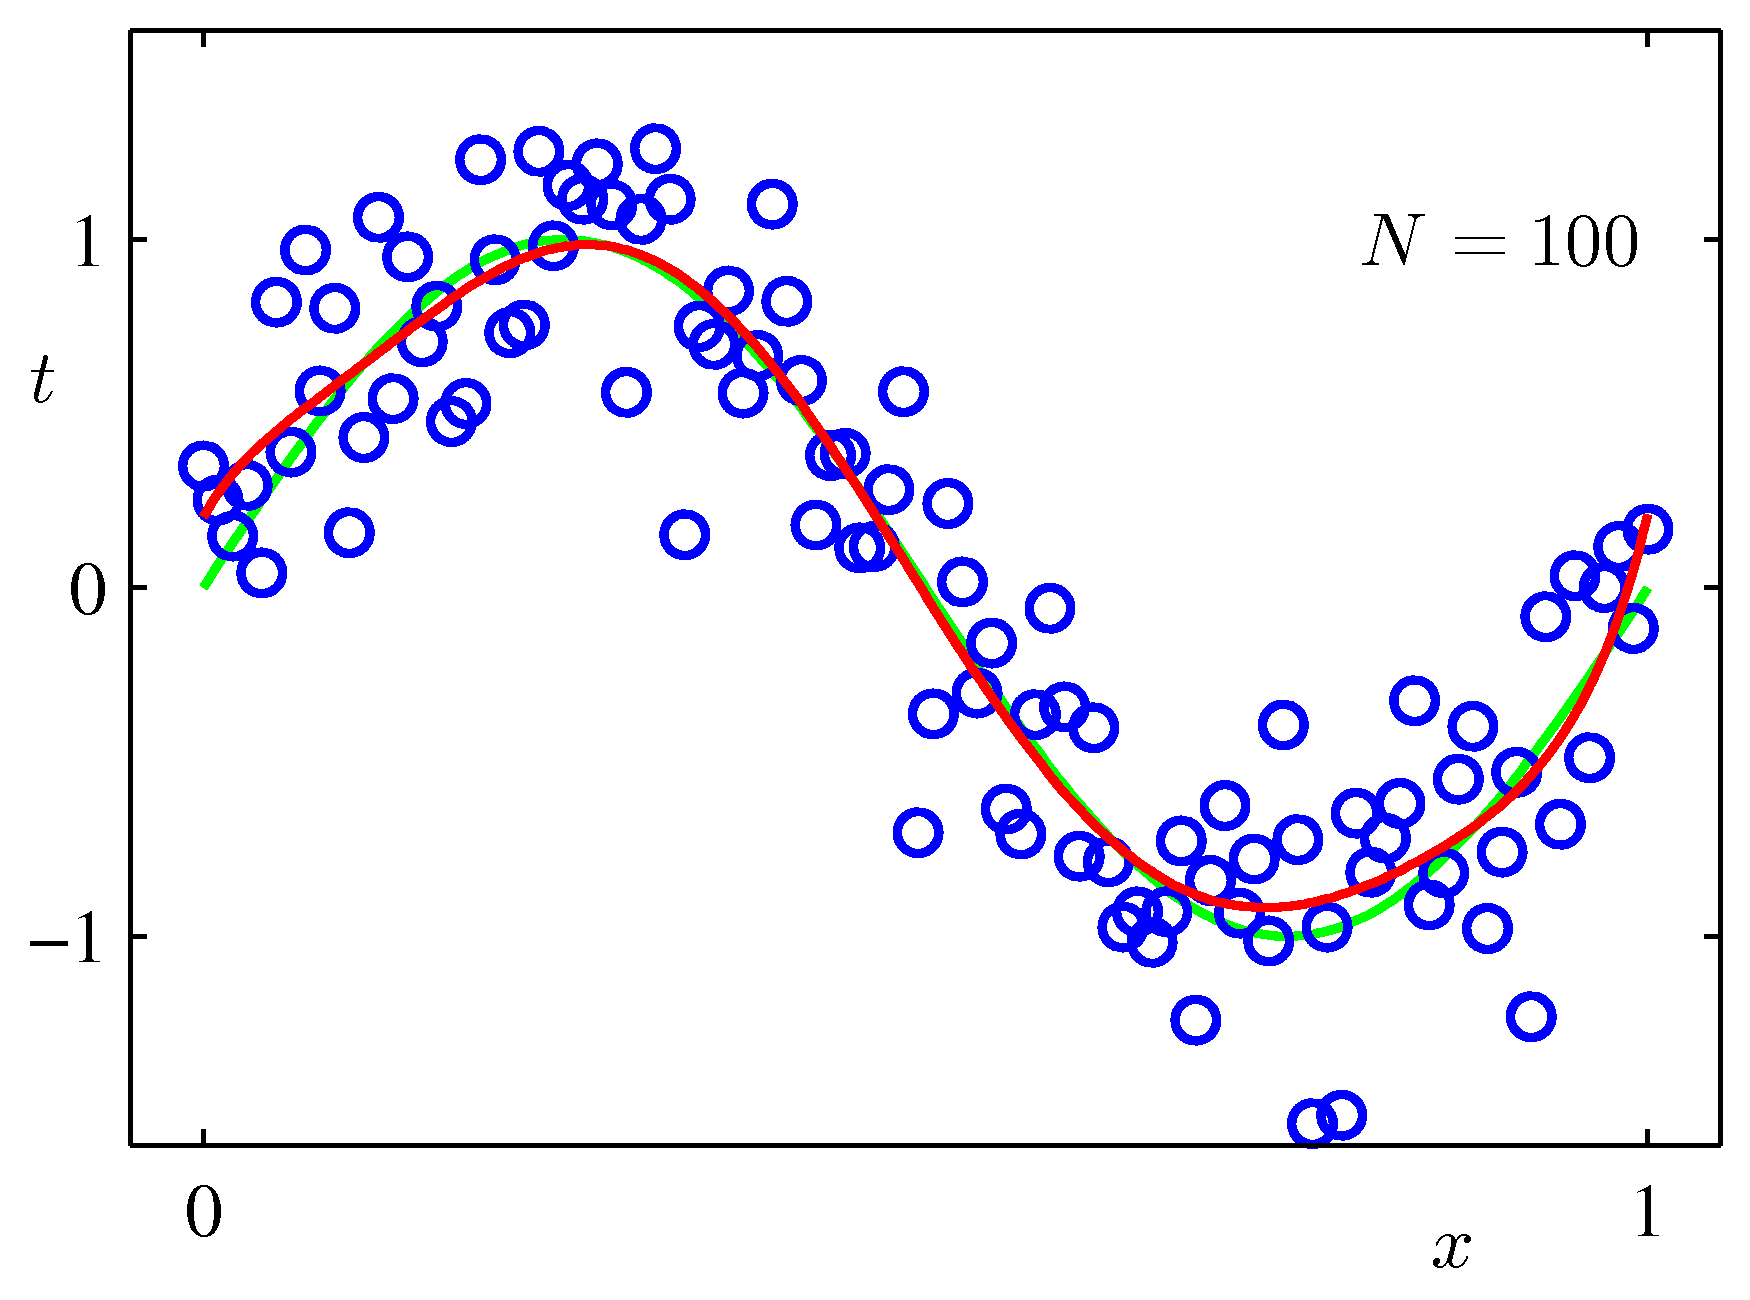
\includegraphics[scale=0.8]{Images/1-6b.png}
		\label{fig:1-6b}
		\end{minipage}
		\captionsetup{font={small}}
		\caption{在$M=9$的情况下,基于$N=15$(左)和$N=100$(右)个数据点进行平方和误差函数最小化得到的结果图像。我们可以看到,数据集规模的增加削弱了过拟合的问题。}
	\end{figure}
	\begin{figure}[H]
		\begin{minipage}[t]{0.5\linewidth}
		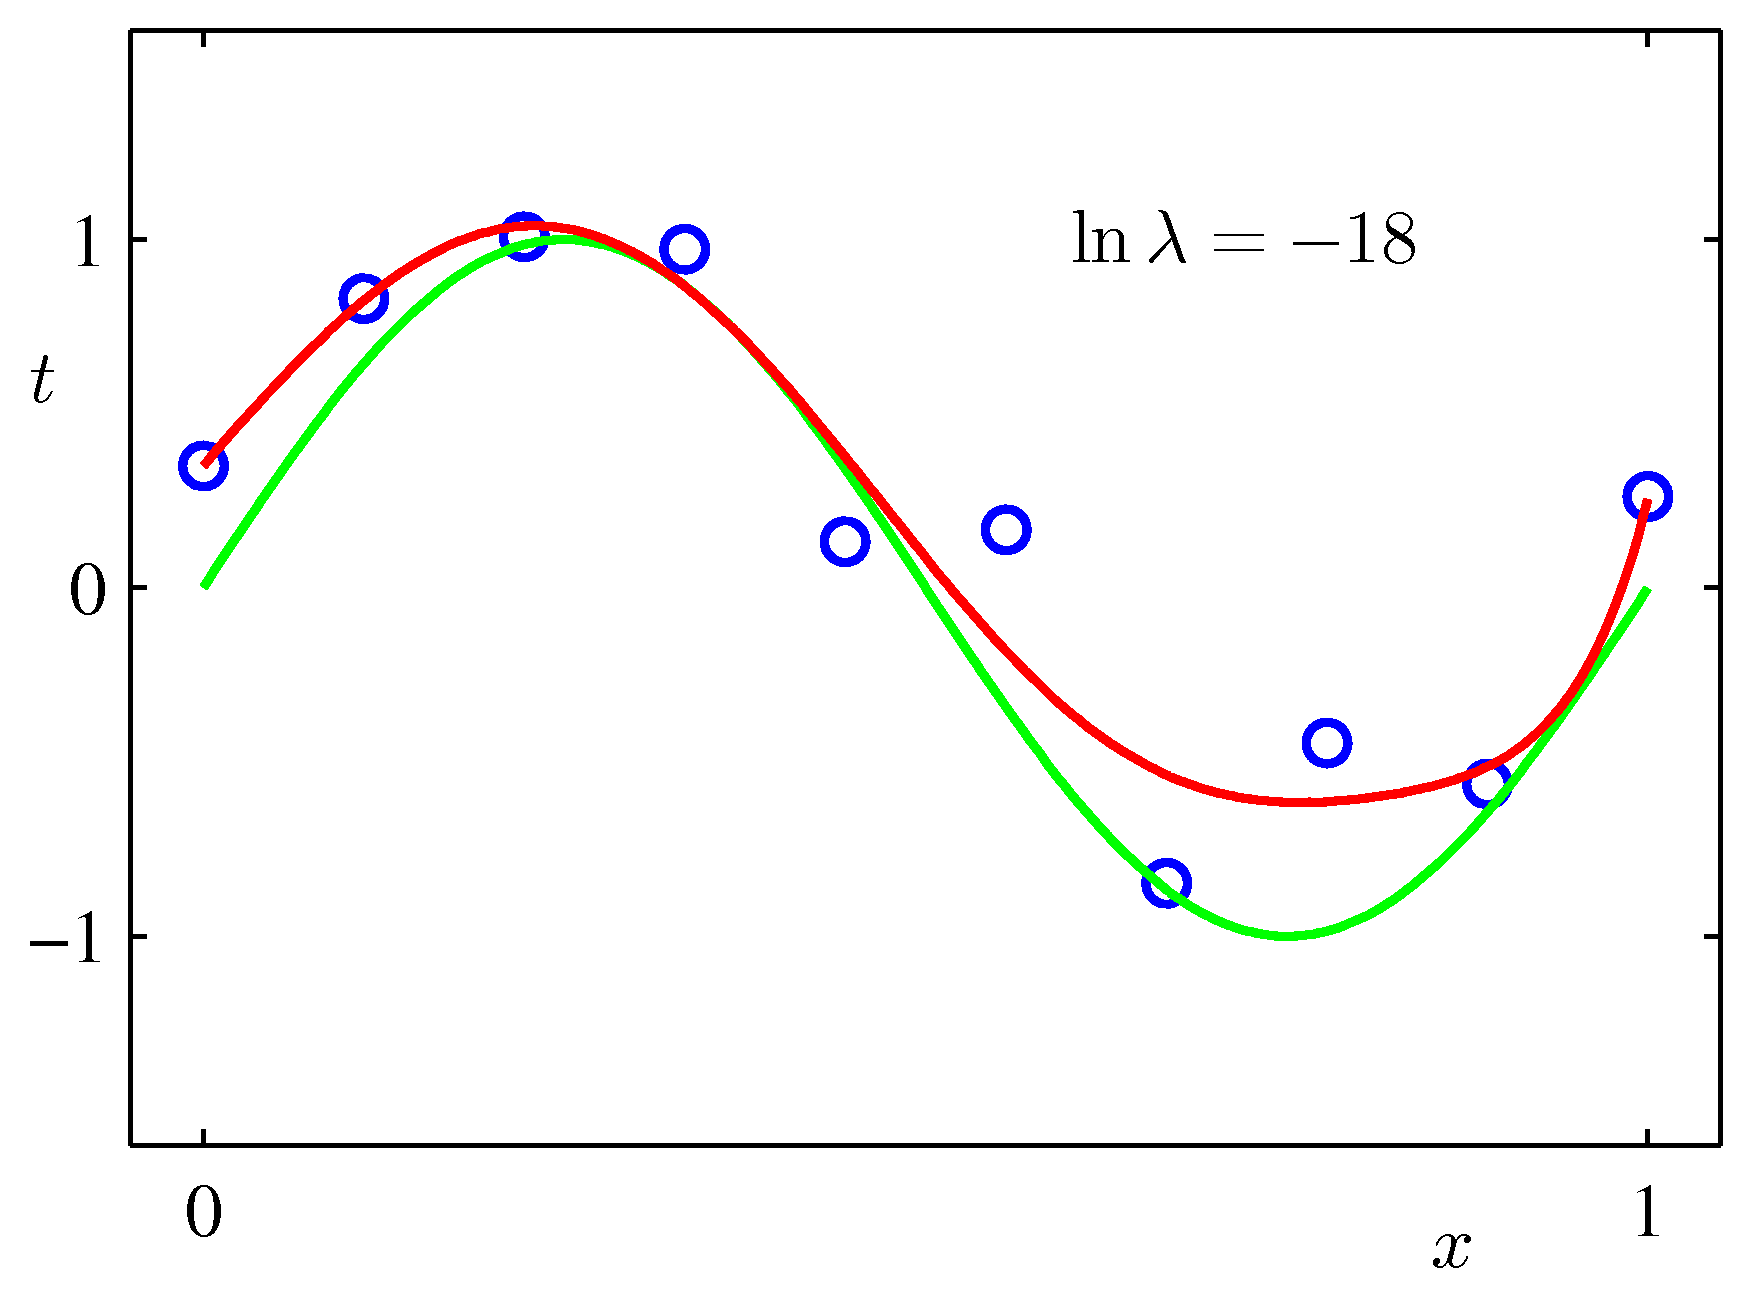
\includegraphics[scale=0.8]{Images/1-7a.png}
		\label{fig:1-7a}
		\end{minipage}
		\begin{minipage}[t]{0.5\linewidth}
		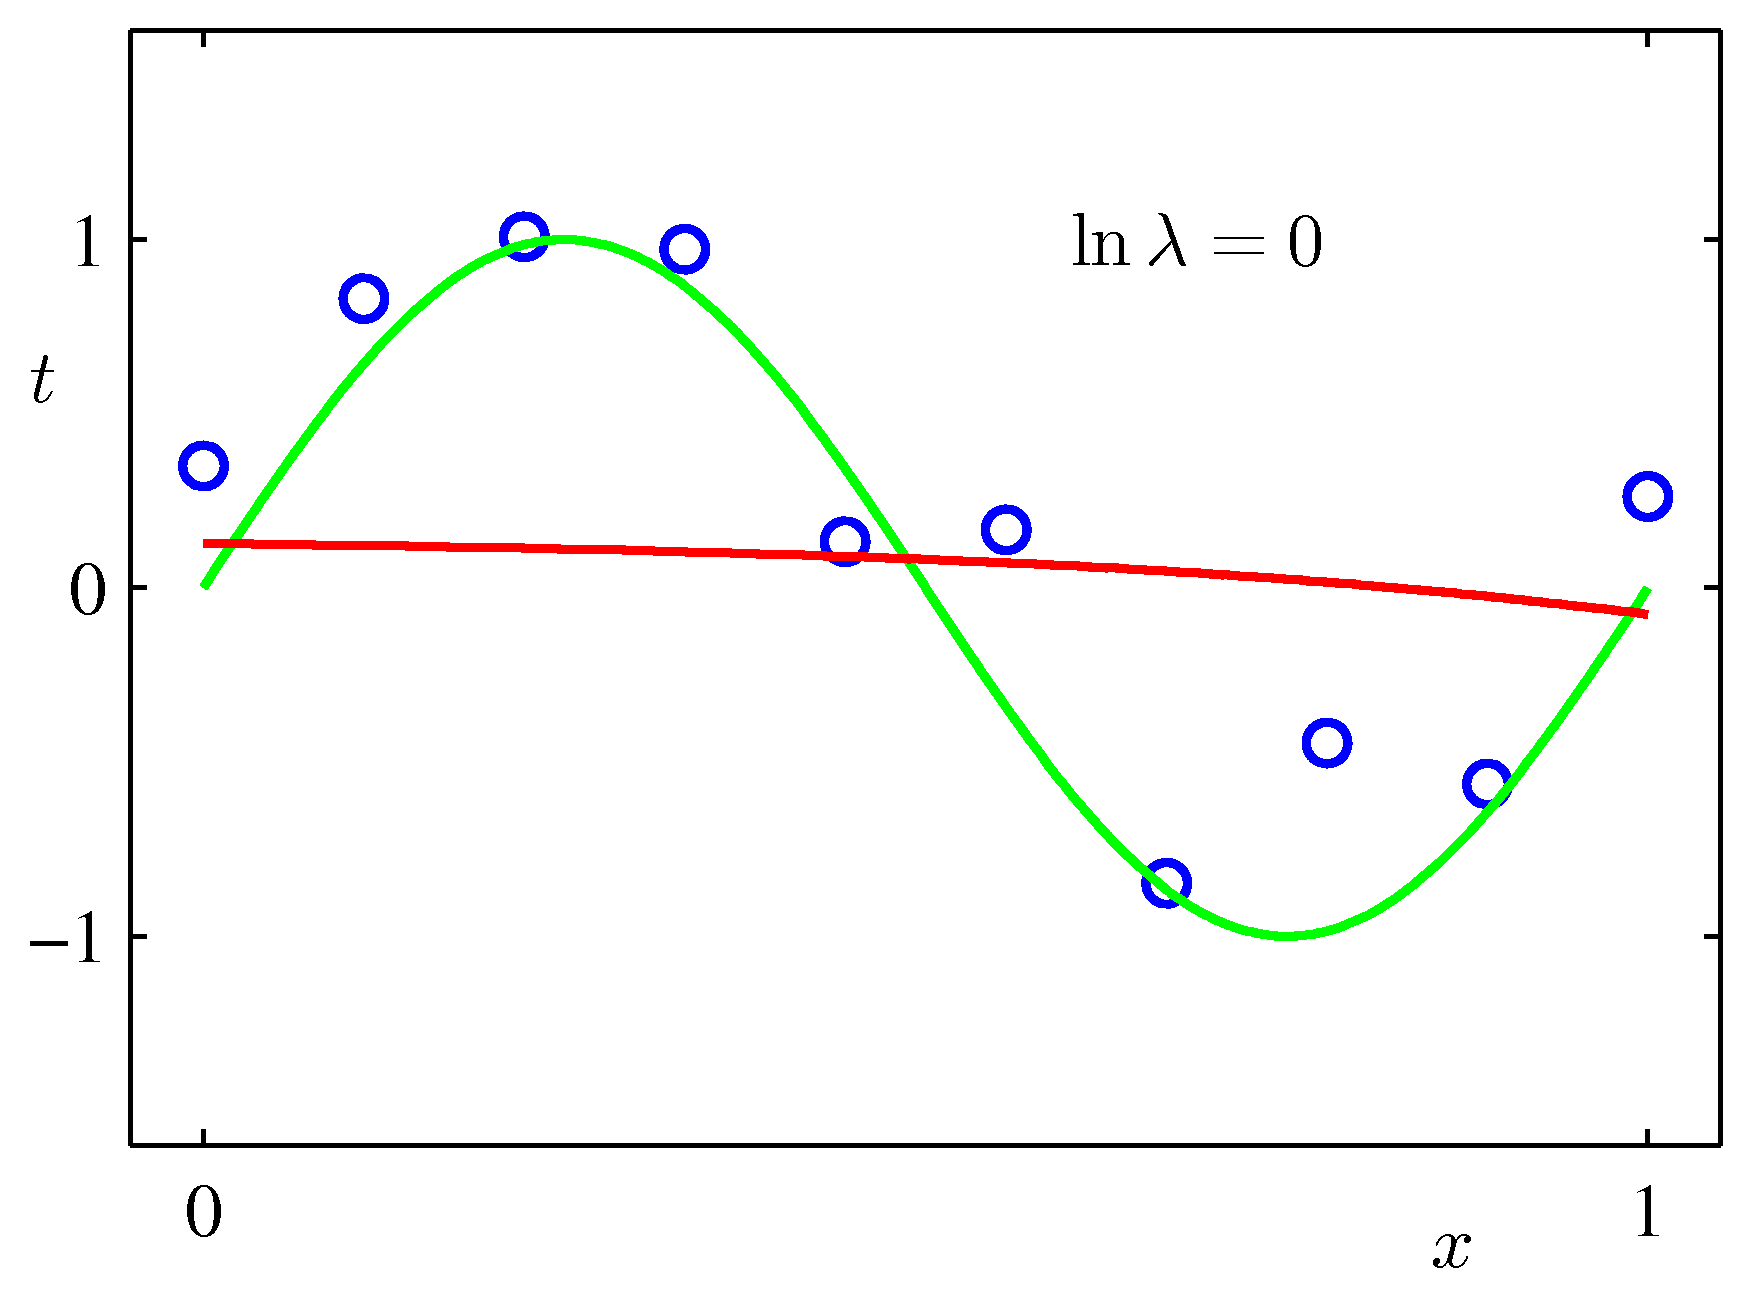
\includegraphics[scale=0.8]{Images/1-7b.png}
		\label{fig:1-7b}
		\end{minipage}
		\captionsetup{font={small}}
		\caption{在$M=9$的情况下,使用(1.4)中的正则化误差函数对图1.2所示的数据集进行拟合,并将正则化参数$\lambda$设置为$\ln \lambda = -18$和$\ln \lambda = 0$。没有正则化的情况(即$\lambda=0$,$\ln \lambda = -\infty$)如图1.4中的右下图所示。}
	\end{figure}
	\noindent 属性之一。\color{red} \textbf{——第3.4节} \color{black}通过使用贝叶斯(Bayesian)方法,可以有效地避免过拟合问题。我们将看到,即使参数数量超过数据点数量,也不会对贝叶斯观点在模型中的应用造成任何困难。其实在贝叶斯模型中,有效(effective)参数的数量将根据数据集的规模进行自发的调整。
	\indent 不过现在的工作也是有意义的,所以还是继续使用目前的方法,并研究如何在现实中将复杂且灵活的模型应用于规模有限的数据集。处理这种过拟合情况的一种常见方法是正则化(regularization),这种方法是在(1.2)中的误差函数里加入惩罚项,从而使系数不会达到太大的值。最简单的惩罚项是对所有系数取平方和,从而得到了如下经过修正的误差函数:
	\begin{equation}
		\widetilde{E}(\mathbf{w})=\frac{1}{2}\sum_{n=1}^{N} \{ y(x_n,\mathbf{w}) - t_n\}^2 + \frac{\lambda}{2} \| \mathbf{w} \|^2
	\end{equation}
	其中$\| \mathbf{w} \|^2 \equiv \mathbf{w^\mathrm{T} w} = w_0^2 + w_1^2 + ... + w_M^2$,系数$\lambda$控制的是正则项与平方和误差项相比之下的真实权重。需要注意的是,在正则式中系数$w_0$通常被省略,因为如果将它包含进来,可能会导致最终结果受到目标变量原点的影响(Hastie et al., 2001),如果要将其包含在内,该项就必须有自己的正则化系数(我们将在第5.5.1节中详细讨论这个话题)。与前面类似,(1.4)中的误差函数可以求取其最小化结果的解析解。\color{red} \textbf{——习题1.2} \color{black}由于系数的值变小了,所以诸如此类的技术在统计学中称为收缩(shrinkage)方法。这种二次正则器被称为岭回归(ridge regression, Hoerl and Kennard, 1970)。在神经网络中,这样的方法称为权重衰减(weight decay)。 \\
	\indent 图1.7展示了阶数$M=9$的多项式对相同数据集的拟合结果,只不过现在使用的误差函数是(1.4)中所示的带有正则项的误差函数。可以看出在$\ln \lambda = -18$时过拟合现象得到了有效的控制,我们得到了一个更加接近原函数$\sin (2 \pi x)$的拟合。但是如果将$\lambda$的值设得太大,我们又会得到一个很差的拟合结果,如图1.7中所示的是$\ln \lambda = 0$的情况。不同正则化参数对应的多项式系数拟合结果如表1.2所示,正则化有效地使多项式的系数变小了很多。\\
	\indent 在图1.8中,通过将训练集和测试集的RMS误差(1.3)各自与$\ln \lambda$的关系绘制在一起,可以看出正则项对泛化误差的影响。可以看出,现在参数$\lambda$有效控制了模型的复杂度,所以决定了过拟合的程度。\\
	\indent 模型复杂度是一个相当重要的问题,我们将在第1.3节中讨论。现在我们只简单地提一句,如果我们希望利用误差函数最小化的方法解决实际问题,就必须要找到一种能够确定合适的模型复杂度的方法。以上的结果算是提出了解决这一问题的一种简单方法,即通过将现有数据划分为训练集(用于确定系数$\mathbf{w^\star}$)和单独的验证集(validation set,亦称拿出集,hold-out set),用于模型复杂度的优化($M$或$\lambda$)。但在很多的场合中,这样的做法是对训练数据的浪费,我们需要寻求更加高级的方法。\color{red} \textbf{——第1.3节} \color{black}\\
	\begin{table}
		\centering
		\begin{tabular}{c|rrr}
			\ & $\ln \lambda = - \infty $ & $\ln \lambda = -18$ & $\ln \lambda = 0$ \\
			\hline
			$w_0^\star$ & 0.35 & 0.35 & 0.13 \\
			$w_1^\star$ & 232.37  & 4.74 & -0.05 \\
			$w_2^\star$ & -5321.83  & -0.77  & -0.06 \\
			$w_3^\star$ & 48568.31  & -31.97  & -0.05 \\
			$w_4^\star$ & -231639.30  & -3.89  & -0.03  \\
			$w_5^\star$ & 640042.26  & 55.28  & -0.02  \\
			$w_6^\star$ & -1061800.52  & 41.32  & -0.01  \\
			$w_7^\star$ & 1042400.18  & -45.95  & -0.00  \\
			$w_8^\star$ & -557682.99  & -91.53  & 0.00  \\
			$w_9^\star$ & 125201.43  & 72.68  & 0.01  \\
		\end{tabular}
		\captionsetup{font={small}}
		\caption{在$M=9$的情况下,不同的正则化参数$\lambda$对应的多项式系数$\mathbf{w^\star}$。需要注意的是,$\ln \lambda = - \infty$对应的是图1.4中所示的无正则化的模型。可以看到,随着$\lambda$的增大,系数的大小会随之减小。}
	\end{table}
	\begin{figure}[H]
		\centering
		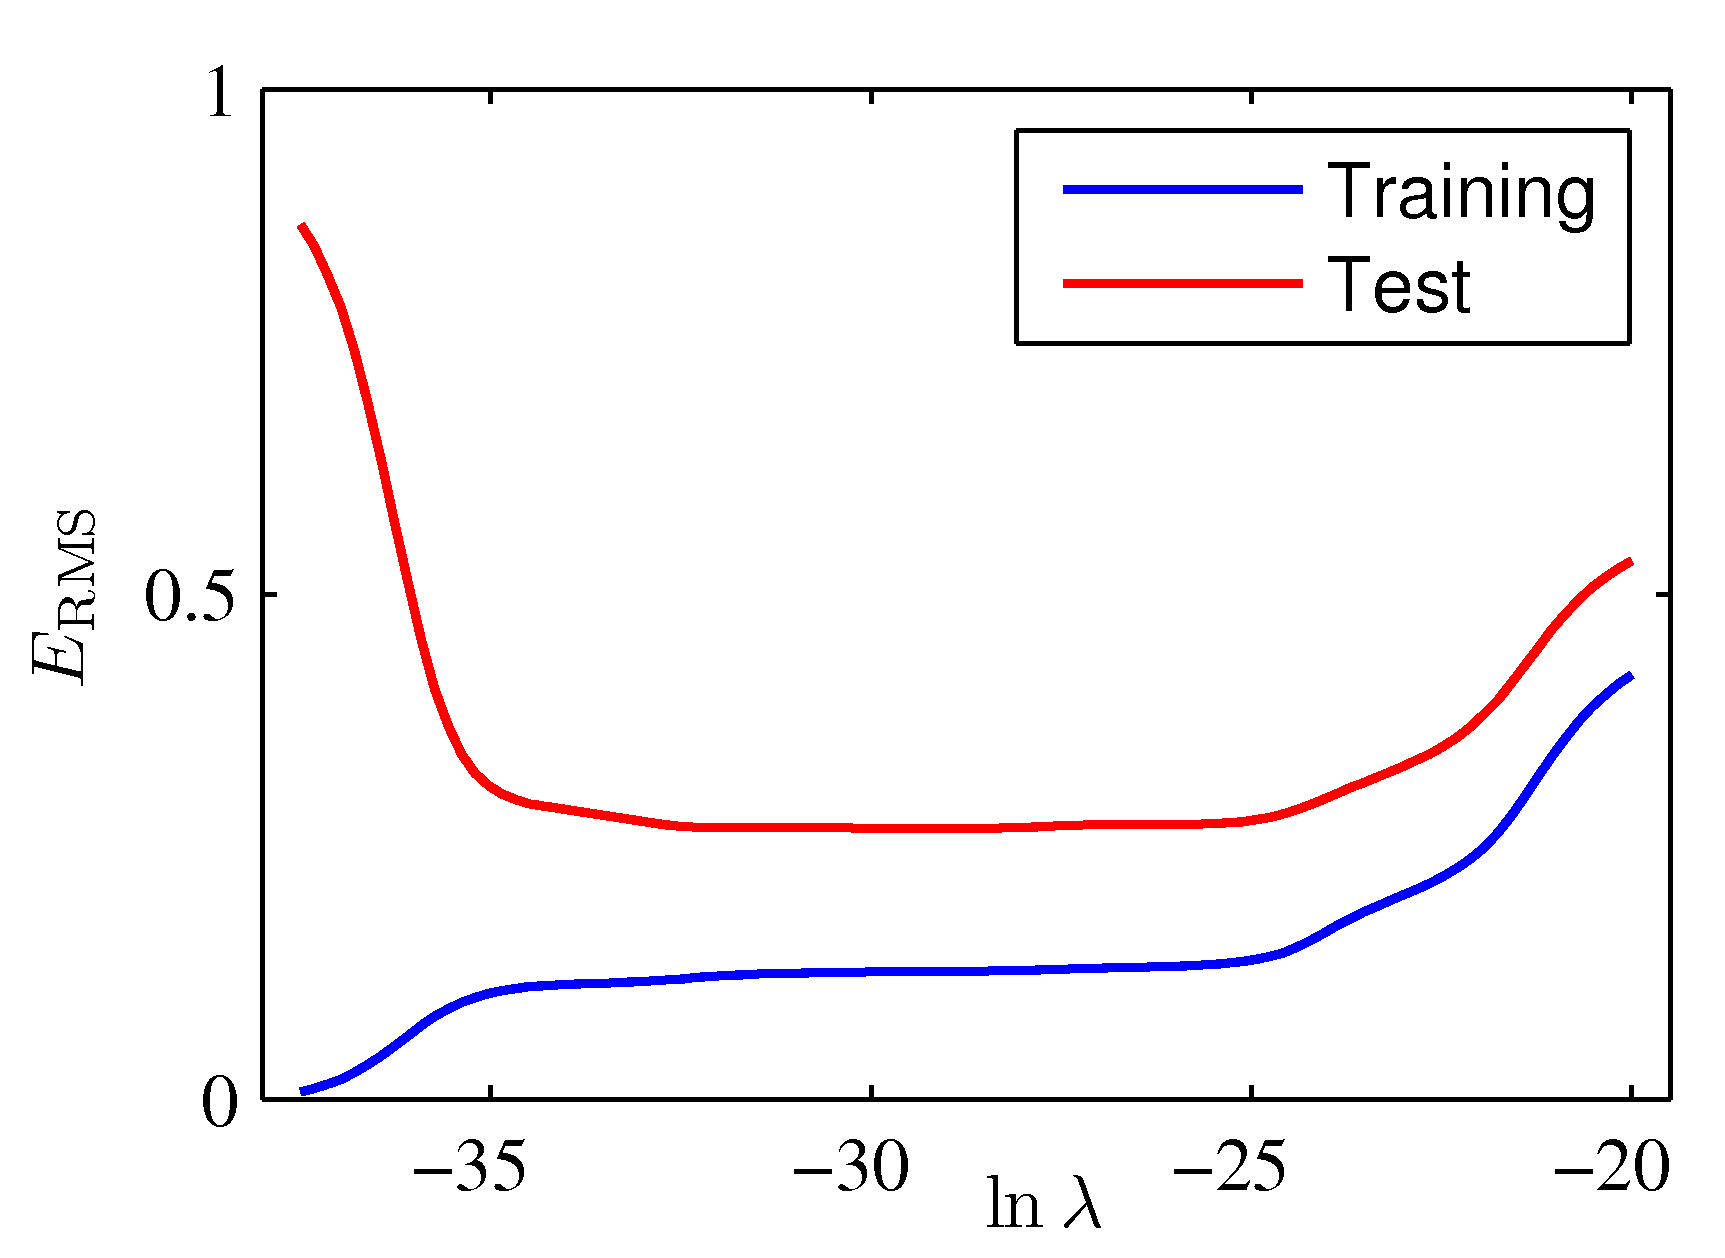
\includegraphics[scale=0.8]{Images/1-8.png}
		\captionsetup{font={small}}
		\caption{在$M=9$的情况下,均方根误差(1.3)随着$\ln \lambda$的变化情况。} 
		\label{fig:1-8}	
	\end{figure}
	到目前为止,关于多项式拟合的讨论很依赖于直觉。我们现在要用更加具体的方法来解决模式识别的问题,那就是概率论。概率论不仅为本书几乎所有的后续章节提供了基础,还能让我们更深刻地理解本章中我们通过多项式拟合的问题引出的重要概念,让我们能够把这些概念扩展到更复杂的情况。
	}
	\section{概率论}
	\noindent{\color{red} \rule[10pt]{\textwidth}{0.1em}}
	\textnormal{
	\indent 在模式识别领域中,最关键的概念之一就是不确定性。不确定性会随着观测噪声和数据集的规模而变化。概率论对于不确定性的量化和计算提供了一个合理的框架,并成为了模式识别的核心基础之一。将概率论与决策论(第1.5节)相结合,我们就可以利用现有的信息进行最优的预测,即使这些信息是不完整的或很含糊的也没关系。\\
	\indent 我们将通过一个简单的例子介绍概率论的一些基础概念。假设我们有两个箱子,一个是红色的,一个是蓝色的,在红色箱子里有2个苹果和6个橙子,在蓝色箱子里有3个苹果和1个橙子,如图1.9所示。假设现在要随机选择一个箱子,并从这个箱子中随机取出一个水果,观察一下是哪一种之后放回原来的箱子里。我们可以假想做了很多次实验。假设我们在40\%的情况下选择红色箱子,60\%的情况下选择蓝色箱子,从箱子中取出哪一个水果是完全等可能的。
	\begin{figure}[ht]
		\centering
		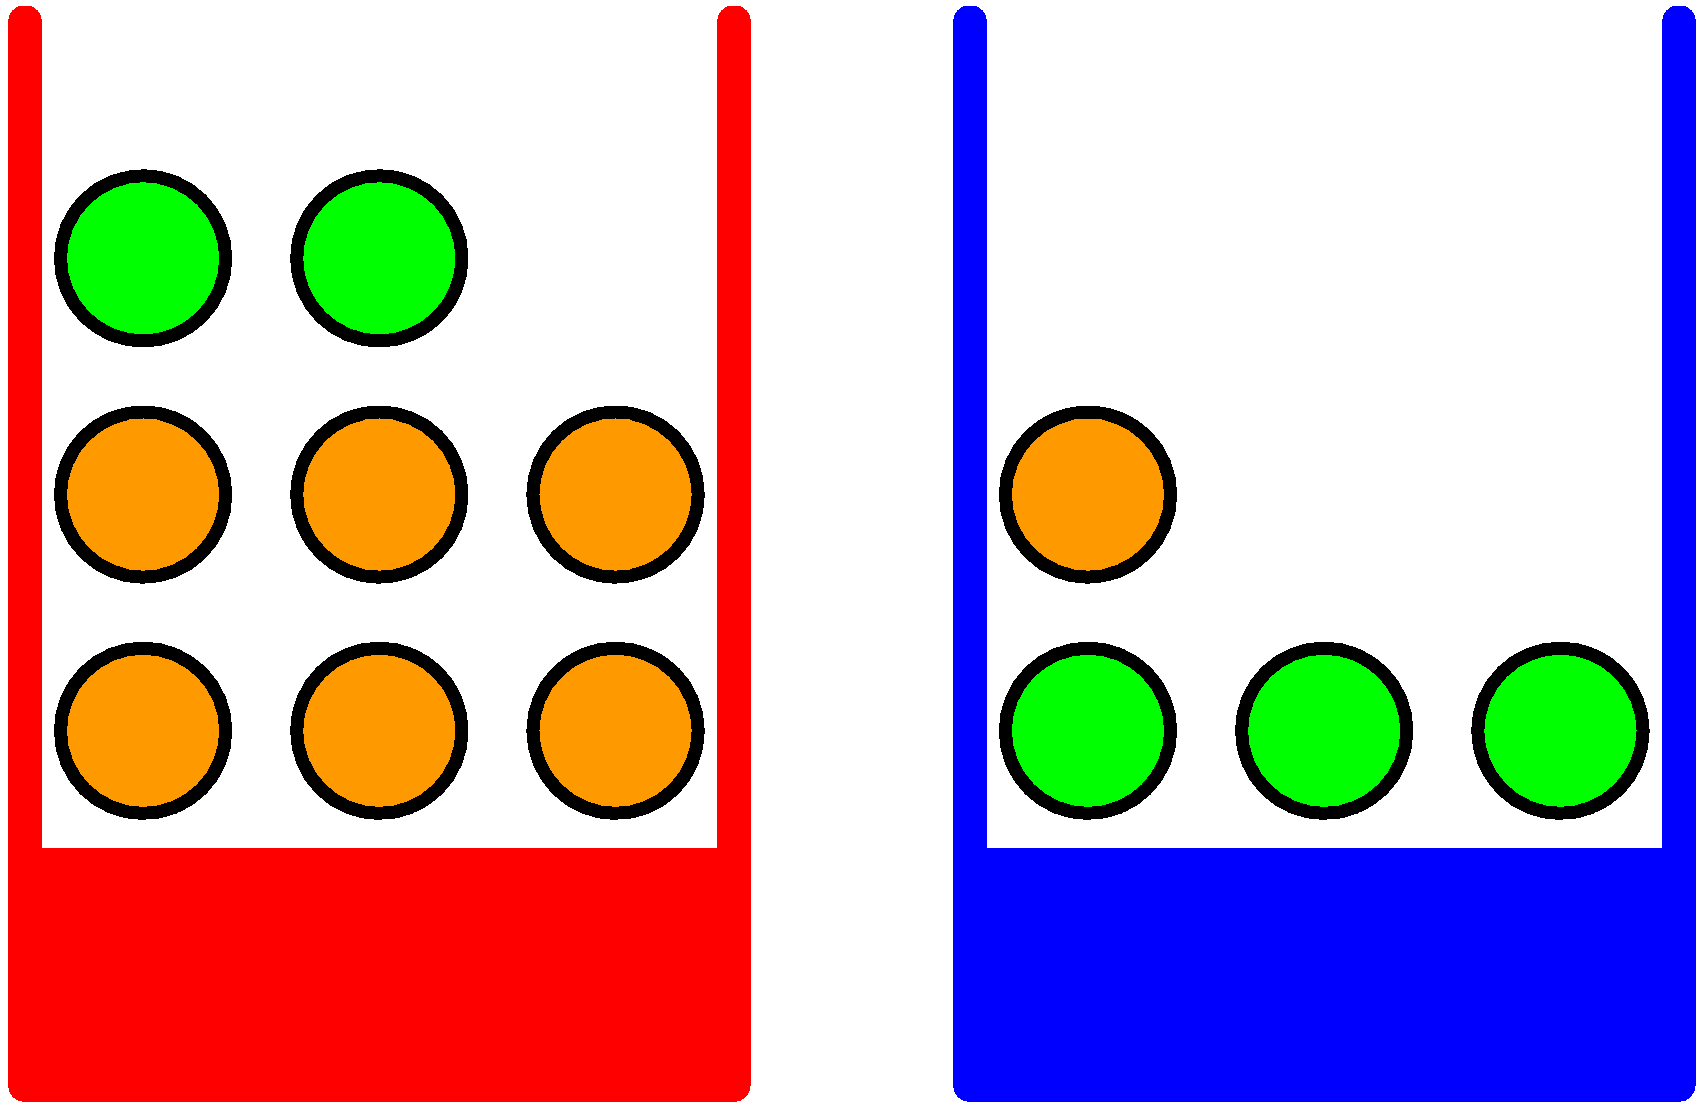
\includegraphics[scale=0.75]{Images/1-9.png}
		\captionsetup{font={small}}
		\caption{我们使用一个简单的小例子来介绍概率论的基础思想,图中是两个不同的箱子,箱子里放着不同类型的水果(绿色的是苹果,橙色的是橙子)。} 
		\label{fig:1-9}	
	\end{figure}
	\\
	\indent 在这个案例中,我们所选择的箱子的特性(颜色)是一个随机变量,记作$B$。这个随机变量有两种可能的取值,即$r$(红色)和$b$(蓝色)。类似地,所选择的水果的特性(种类)也是一个随机变量,记作$F$,其取值同样只有两种可能,即$a$(苹果)或$o$(橙子)。\\
	\indent 从概率的定义出发,我们将一个事件的概率定义为实验次数趋近于无穷时,事件发生的次数与实验总数的比值。于是,选择红色箱子的概率是4/10,选择蓝色箱子的概率是6/10。我们将其记作$p(B=r)=4/10$和$p(B=b)=6/10$。需要注意的是,根据定义,概率必须在区间$[0,1]$内。另外,如果某些事件是相互独立的,而且覆盖了所有可能的输出结果(例如,在这个例子中选择的箱子非红即蓝),那这些事件的概率之和一定等于1。\\
	\indent 现在我们可以问类似这样的问题:“拿到苹果的概率是多少?”或“已知拿到的是橙子,选择的箱子是蓝色箱子的概率是多少?”。这样的问题当然是可以解答的,比这复杂得多的模式识别问题都不在话下,不过首先要掌握加法规则(sum rule)和乘法规则(product rule)两项概率论基本规则。我们将在掌握这两项规则之后,再回到水果箱子案例中。\\
	\indent 为了推导概率中的这些规则,我们考虑一个稍微一般一些的情况,如图1.10所示,该例中包含了两个随机变量$X$和$Y$(类似于上一个例子中的箱子变量和水果变量)。假设$X$的取值可以是任意的$x_i$,其中$i=1,...,M$,$Y$的取值可以是任意的$y_j$,其中$j=1,...,L$。在$N$次实验中,对$X$和$Y$都进行了取样,并将$X=x_i,Y=y_j$的情况发生的次数记作$n_{ij}$。另外,将$X=x_i$的情况发生的次数(忽略$Y$的值)记作$c_i$,类似地将$Y=y_j$的情况发生的次数记作$r_j$。
	\begin{figure}[ht]
		\centering
		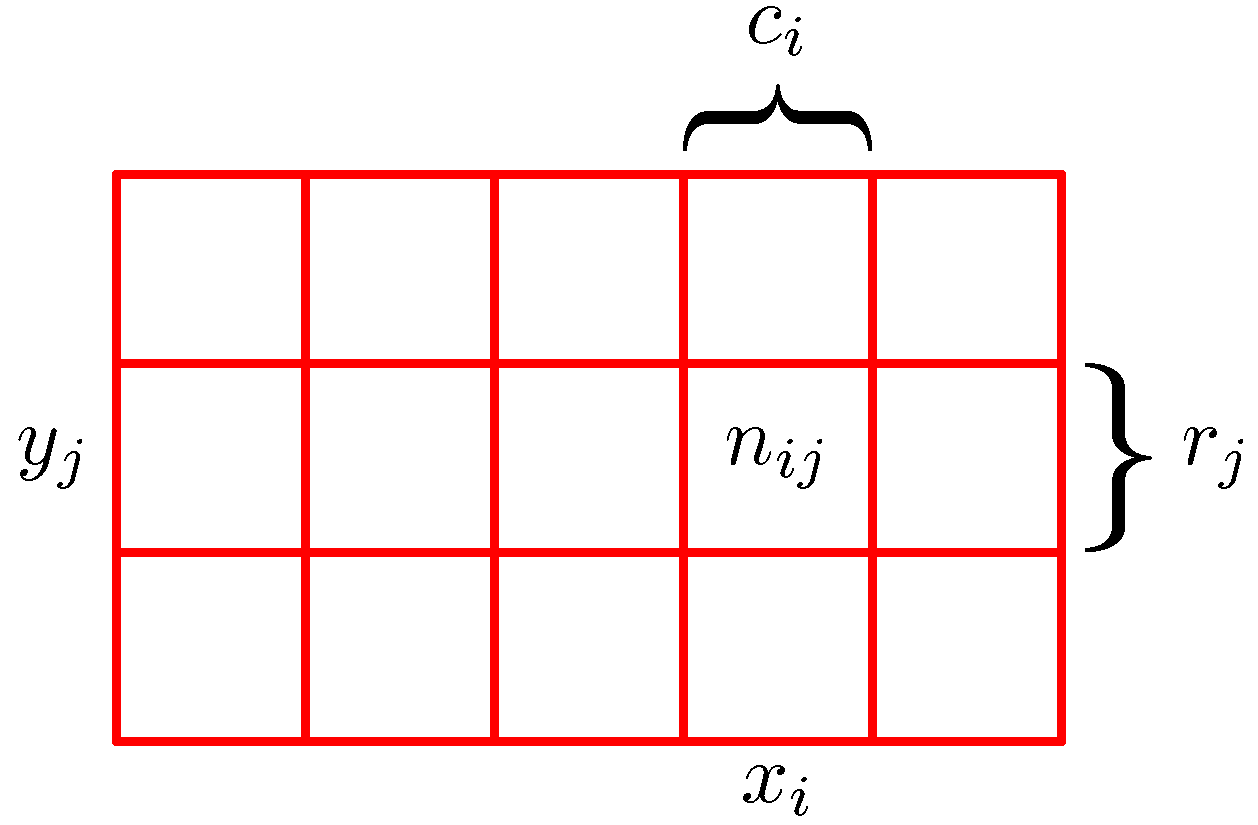
\includegraphics[scale=0.8]{Images/1-10.png}
		\captionsetup{font={small}}
		\caption{我们可以通过这样的例子来推导加法规则和乘法规则,有两个随机变量$X$和$Y$,其中$X$的取值范围是$\{x_i\},i=1,...,M$,$Y$的取值范围是$\{y_j\},j=1,...,L$。假设$M=5,L=3$,总共进行$N$次实验,将$X=x_i$且$Y=y_j$的次数记作$n_{ij}$,也就是落在相应单元格内的结果总数。在第$i$列中的点数对应的是$X=x_i$的情况发生的次数,记作$c_i$,在第$j$行中的点数对应的是$Y=y_j$的情况发生的次数,记作$r_j$。} 
		\label{fig:1-10}
	\end{figure}
	\\
	\indent $X=x_i$且$Y=y_j$的情况发生的概率称为$X=x_i$和$Y=y_j$的联合概率(joint probability),记作$p(X=x_i,Y=y_j)$。联合概率由落入$(i,j)$单元格中的结果数量与总实验次数求取比值得到,即:
	\begin{equation}
		p(X=x_i,Y=y_j)=\frac{n_{ij}}{N}
	\end{equation}
	\indent 在这里我们比较隐晦地认为$N$是趋近于无穷的。类似地,既然$X=x_i$的概率是与$Y$的取值无关的,所以就是第$i$列中的结果总数与实验总数的比值,那么$p(X=x_i)$就可以写成:
	\begin{equation}
		p(X=x_i)=\frac{c_i}{N}
	\end{equation}
	\indent 由于图1.10中第$i$列中的结果总数就是该列中每一个单元格里结果数的总和,于是有$c_i=\sum_{j}n_{ij}$,所以根据(1.5)和(1.6),可以得到:
	\begin{equation}
		p(X=x_i)=\sum_{j=1}^{L} p(X=x_i,Y=y_j)
	\end{equation}
	\indent 这就是概率的加法规则。需要注意的是,有时$p(X=x_i)$被称为边缘概率(marginal probability),因为它是通过将其他变量(在这个例子中是$Y$)进行边缘化(或者说求和)得到的。\\
	\indent 如果仅考虑$X=x_i$的情况,在这样的限制下$Y=y_j$的结果数在$X=x_i$的结果中所占的比例被称为给定$X=x_i$的$Y=y_j$的条件概率(conditional probability),记作$p(Y=y_j|X=x_i)$。条件概率要通过计算$(i,j)$单元格中的结果数与第$i$列中的结果总数的比值得到,即:
	\begin{equation}
		p(Y=y_j|X=x_i)=\frac{n_{ij}}{c_i}
	\end{equation}
	\indent 根据(1.5),(1.6)和(1.8),我们可以进行如下推导:
	\begin{equation}
		p(X=x_i,Y=y_j) = \frac{n_{ij}}{N}=\frac{n_{ij}}{c_i} \cdot \frac{c_i}{N} = p(Y=y_j|X=x_i)p(X=x_i)
	\end{equation}
	\indent 这就是概率的乘法规则。\\
	\indent 到目前为止我们一直都比较小心地将随机变量(比如水果箱子案例中的箱子变量$B$)和随机变量可能的取值(比如$B=r$)区分开来。所以,$B$的取值为$r$的概率可以记为$p(B=r)$。尽管这样讲可以避免歧义,但真的很是繁琐,而且很多情况下确实不需要这样刻板。所以我们不用这样的写法,而是将随机变量$B$的分布记作$p(B)$,将该分布取特定值$r$的估计记作$p(r)$,这样就清楚得多了。\\
	\indent 有了这样更加简练的表示,我们可以将概率论的两条基本规则写成如下的形式:\\
	\insertline\\
	\color{red} $\bullet$ \textbf{\ 概率论的基本规则} \color{black}
	\begin{align}
		\textbf{加法规则(sum rule)\ \ \ \ } &p(X)=\sum_{Y}^{}p(X,Y) \\
		\textbf{乘法规则(product rule)\ \ \ \ } &p(X,Y)=p(Y|X)p(X)
	\end{align}
	\insertline\\
	\indent 这里的$p(X,Y)$表示的是联合概率,也就是“$X$且$Y$的概率”。类似地,$p(Y|X)$表示的是条件概率,也就是“在$X$的情况下$Y$的概率”,$p(X)$为边缘概率,也就是“$X$的概率”。这两项基础规则构成了概率论的基础,会在本书中贯穿始终。\\
	\indent 从乘法规则出发并引入对称性$p(X,Y)=p(Y,X)$,我们马上就可以得到条件概率之间的如下关系:
	\begin{equation}
		p(Y|X)=\frac{p(X|Y)p(Y)}{p(X)}
	\end{equation}
	\indent 这就是著名的贝叶斯定理(Bayes' theorem),它在模式识别和机器学习中扮演了核心的角色。利用加法规则,贝叶斯定理中的分母可以表示为:
	\begin{equation}
		p(X)=\sum_{Y}^{} p(X|Y)p(Y)
	\end{equation}
	\indent 可以看出贝叶斯定理中的分母其实是一个归一化常数,保证了(1.12)等式左侧满足$Y$的全部取值的条件概率之和为1。\\
	\indent 在图1.11中,我们展示了一个包含两个变量的联合分布的案例来解释边缘分布(marginal distribution)和条件分布(conditional distribution)的概念。其中,左上方的图展示了一个从联合分布中抽取的包含有$N=60$个数据点的有限样本。右上方的直方图展示了两种取值的$Y$各自所占的比例。根据概率的定义,在$N\rightarrow \infty$时,该比例将等于其相应的概率。我们可以将直方图视作在给定了从分布中抽取的有限点的情况下,模拟概率分布的一种简单方法。通过数据对分布进行建模是统计模式识别的核心,在本书中将进行详细的探讨。图1.11中余下的两个图展示了$p(X)$和$p(X|Y=1)$的直方图估计。
	\begin{figure}[ht]
		\begin{minipage}[t]{0.5\linewidth}
		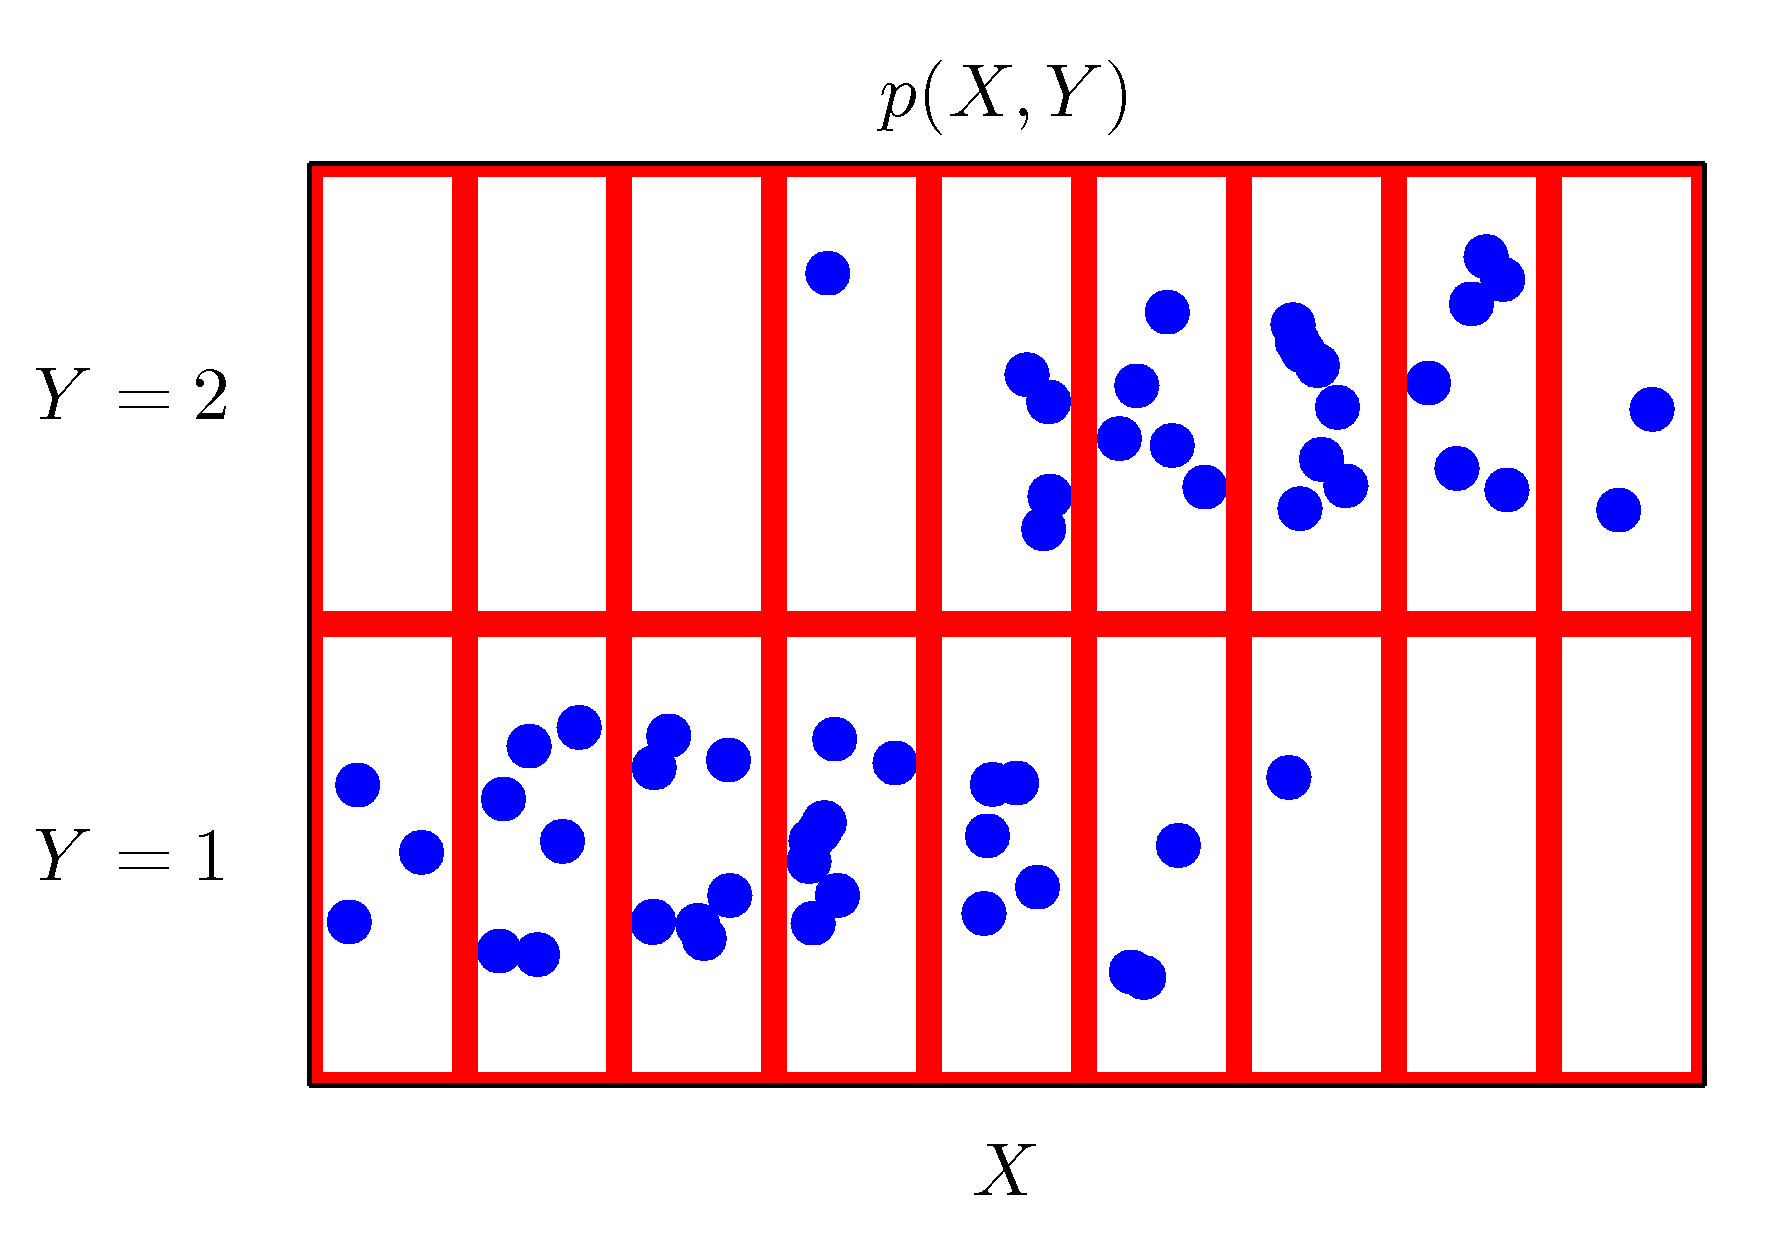
\includegraphics[scale=0.8]{Images/1-11a.png}
		\label{fig:1-11a}
		\end{minipage}
		\begin{minipage}[t]{0.5\linewidth}
		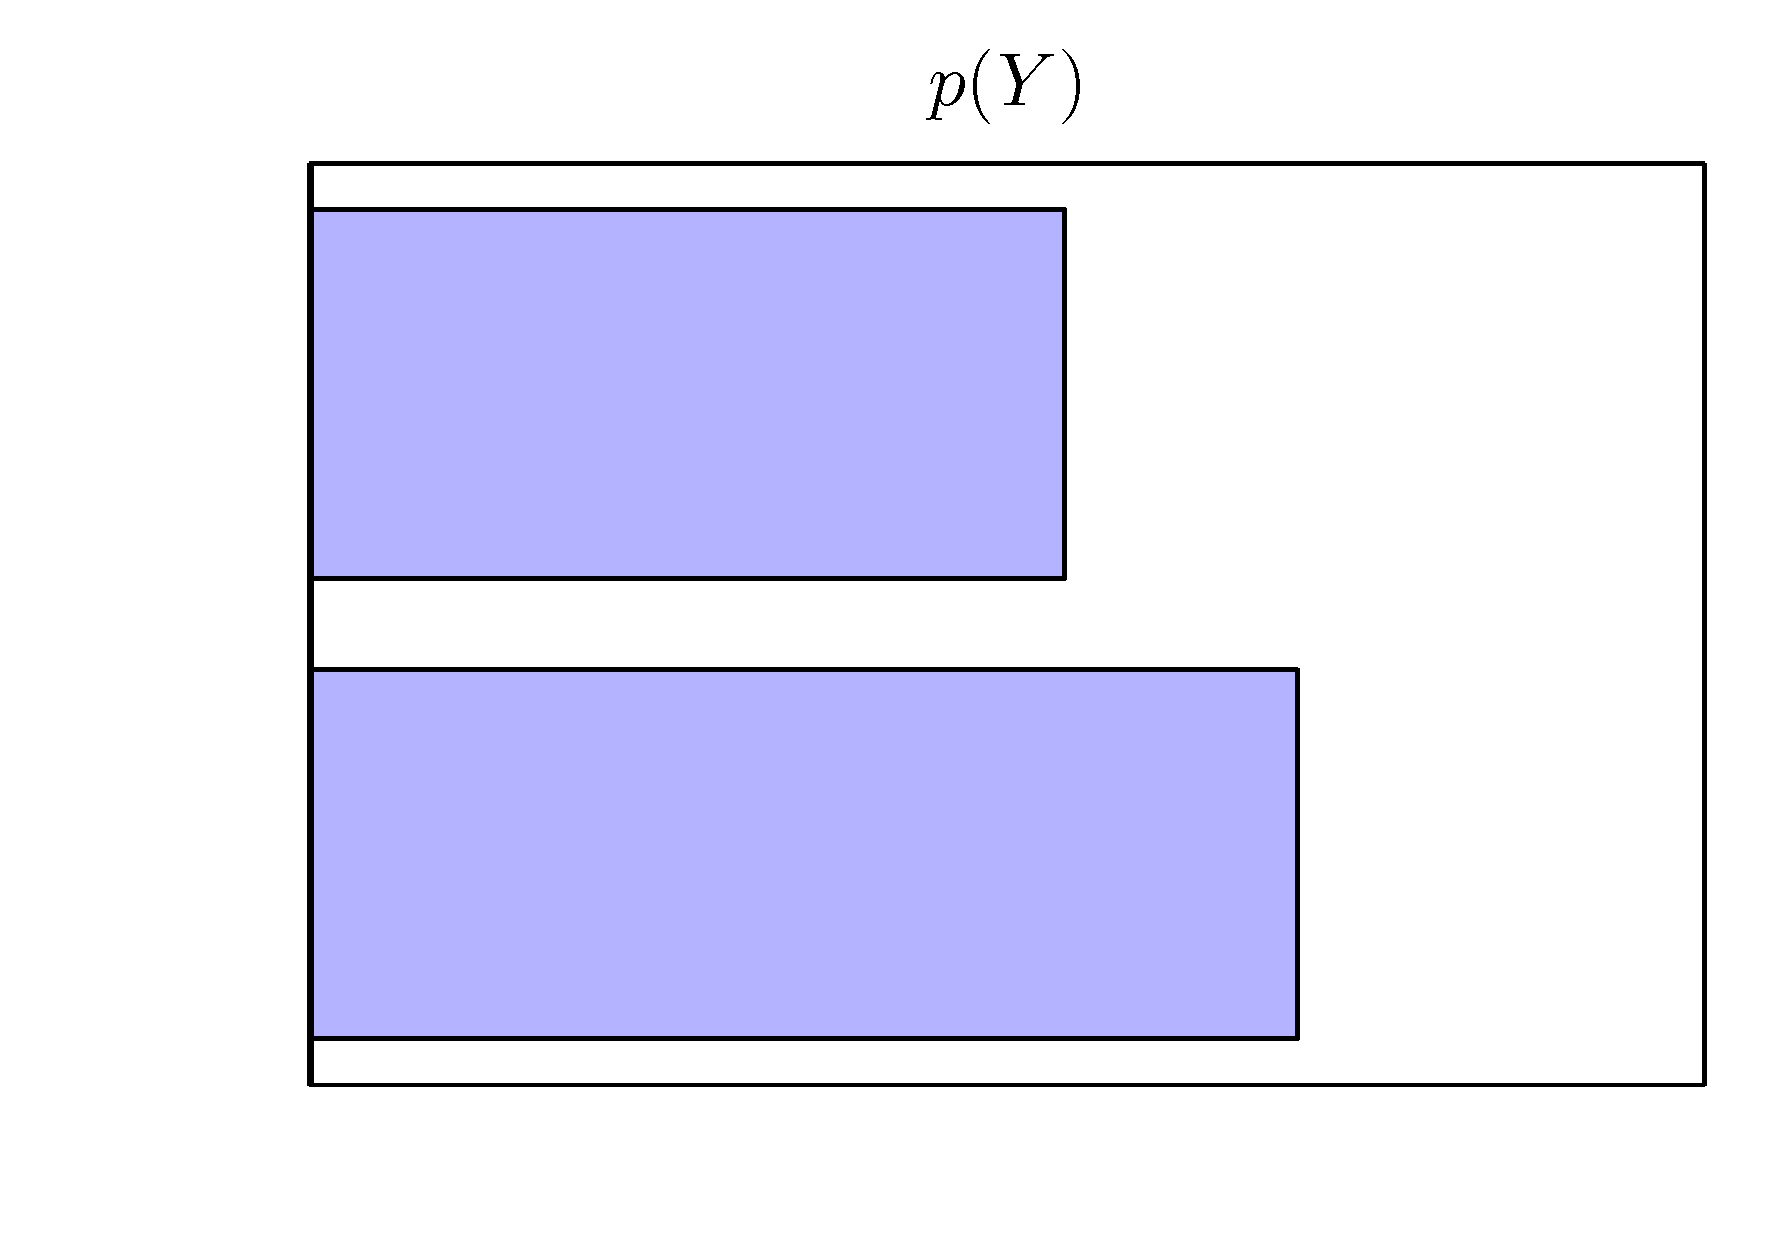
\includegraphics[scale=0.8]{Images/1-11b.png}
		\label{fig:1-11b}
		\end{minipage}\\
		\begin{minipage}[t]{0.5\linewidth}
		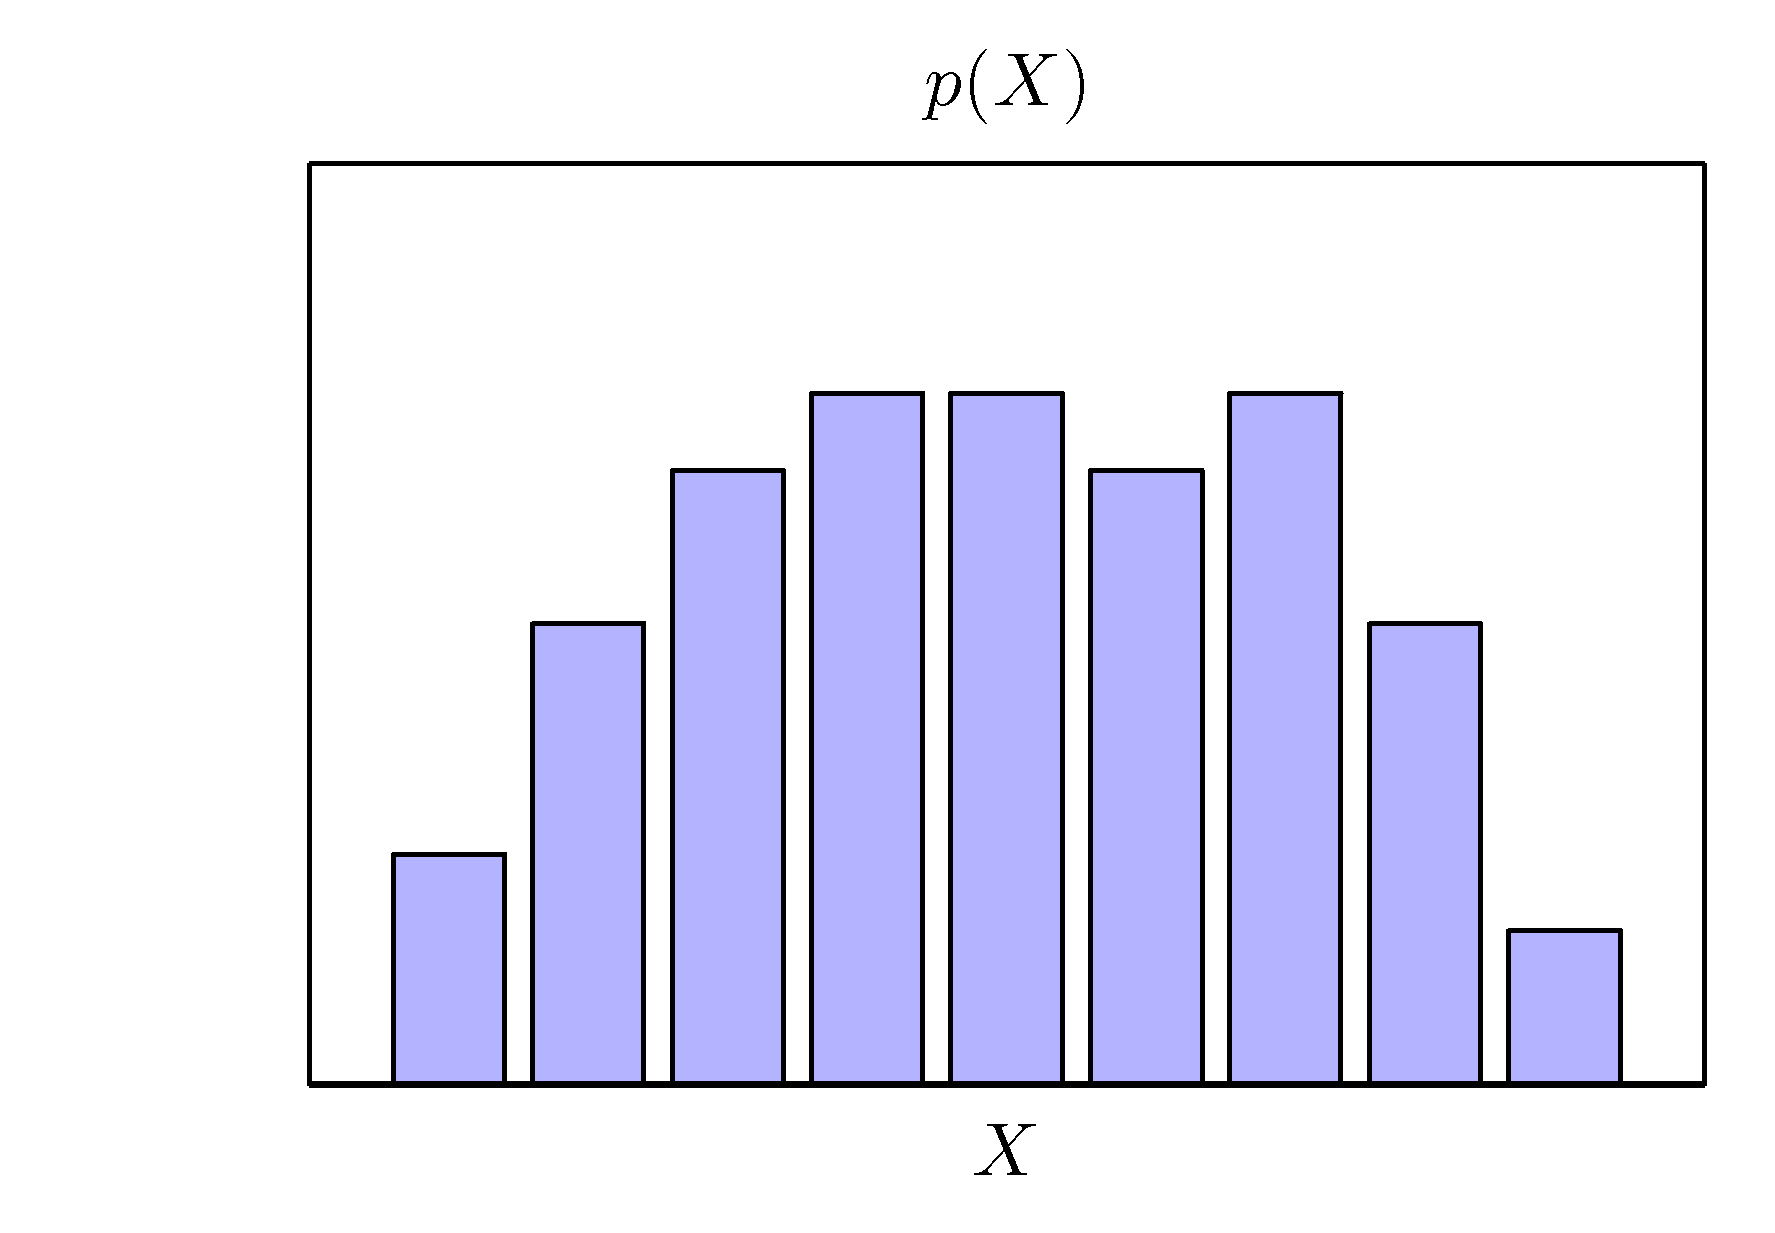
\includegraphics[scale=0.8]{Images/1-11c.png}
		\label{fig:1-11c}
		\end{minipage}
		\begin{minipage}[t]{0.5\linewidth}
		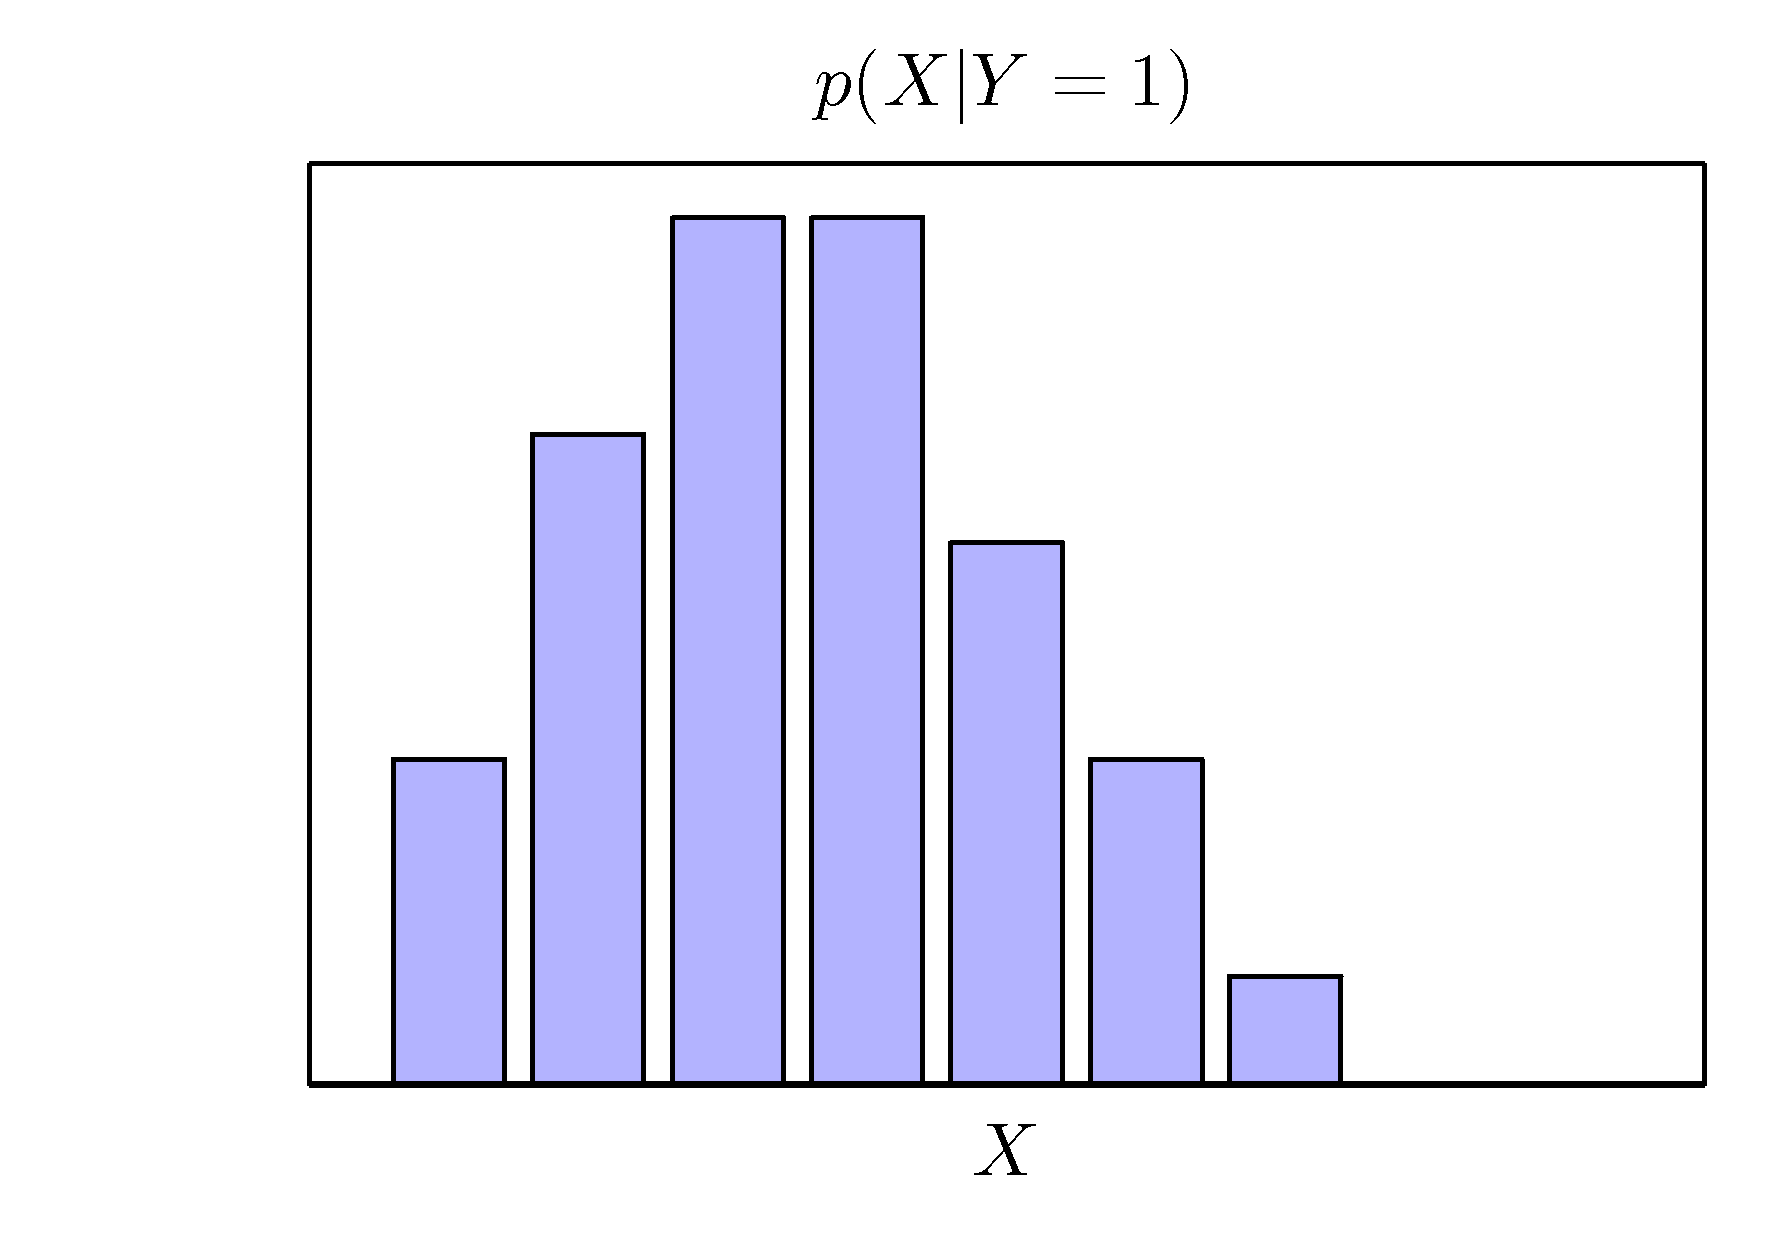
\includegraphics[scale=0.8]{Images/1-11d.png}
		\label{fig:1-11d}
		\end{minipage}
		\captionsetup{font={small}}
		\caption{两个变量的分布图,$X$有9种可能的取值,$Y$有2种可能的取值。左上图显示了从这些变量的联合概率分布中抽取的60个样本点。其余图显示了边缘分布$p(X)$和$p(Y)$的直方图估计,以及对应于左上图中下面一行的条件分布$p(X|Y=1)$。}
	\end{figure}
	\\
	\indent 现在我们回到之前的水果箱子案例中,再次对随机变量与其取值进行区分。选择红色箱子和蓝色箱子的概率分别为:
	\begin{align}
		p(B=r)&=4/10 \\
		p(B=b)&=6/10
	\end{align}
	\indent 注意,$p(B=r)+p(B=b)=1$。\\
	\indent 假设我们随机选择了一个箱子,发现是蓝色的。那么选择到苹果的概率就是蓝色箱子中苹果的比例,即3/4,也就是说$p(F=a|B=b)=3/4$。事实上,我们可以写出给定箱子的情况下,取出水果种类的全部四种概率:
	\begin{align}
		p(F=a|B=r) &=1/4 \\
		p(F=o|B=r) &=3/4 \\
		p(F=a|B=b) &=3/4 
	\end{align}
	\begin{equation}
		p(F=o|B=b) =1/4 
	\end{equation}
	\indent 概率在这里同样是归一化的:
	\begin{align}
		p(F=a|B=r)+p(F=o|B=r) &=1 \\
		p(F=a|B=b)+p(F=o|B=b) &=1
	\end{align}
	\indent 于是我们可以利用加法规则和乘法规则计算完整的取出苹果的概率:
	\begin{equation}
		\begin{split}
			p(F=a) &= p(F=a|B=r)p(B=r)+p(F=a|B=b)p(B=b) \\ 
			&= \frac{1}{4}\times\frac{4}{10}+\frac{3}{4}\times\frac{6}{10} = \frac{11}{20}
		\end{split}
	\end{equation}
	\indent 于是$p(F=o)=1-11/20 = 9/20$。\\
	\indent 假设现在换一种情况,我们已知的是拿到的水果是一个橙子,希望知道是从哪一个箱子里拿出的水果。这就要求我们估计给定水果类别情况下的箱子类别的概率分布,相比之下,(1.16)~(1.19)给出的是给定箱子类别的情况下水果类别的概率分布。我们可以利用贝叶斯定理来求解这个问题:
	\begin{equation}
		p(B=r|F=o)=\frac{p(F=o|B=r)p(B=r)}{p(F=o)}=\frac{3}{4} \times \frac{4}{10} \times \frac{20}{9} = \frac{2}{3}
	\end{equation}
	\indent 根据加法规则,$p(B=b|F=o)=1-2/3=1/3$。\\
	\indent 我们可以给出对于贝叶斯定理的如下重要解释。如果我们要在知晓拿到的水果种类之前预测箱子的类别,那么我们可以利用的最完整的信息来自于$p(B)$。我们将之称为\textbf{先验概率}(prior probability),因为这一项概率是在我们得到水果类别之前就可以获得的。一旦我们被告知了水果的类别(比如说橙子),我们就可以用贝叶斯定理去求取$p(B|F)$,这一项我们称为\textbf{后验概率}(posterior probability),因为我们会在得到$F$之后得到这一概率。注意在这个案例中,选择红色箱子的先验概率是4/10,所以选择蓝色箱子的可能性要大于红色箱子。但是,一旦我们观测到了取出的水果是一个橙子,选择红色箱子的后验概率就是2/3了,所以选择红色箱子的可能性就更大了。这个结果是比较符合我们的直觉的,因为红色箱子中橙子的比例要远大于蓝色箱子的,所以拿出的水果是橙子这一事件为做出选择的箱子是红色箱子这一预测提供了很有利的判据。其实,这项判据强大到以至于盖过了先验,使得选择的箱子更有可能是红色箱子而非蓝色箱子。\\
	\indent 最后,还要注意到,如果两个变量的联合分布可以分解为两个边缘分布的乘积,即$p(X,Y)=p(X)p(Y)$,那么$X$和$Y$就是相互独立的(independent)。根据乘法规则,$p(Y|X)=p(Y)$,所以给定$X$的$Y$的条件分布是完全独立于$X$的。例如,在水果箱子案例中,如果每个箱子中包含相同比例的苹果和橙子,那么$p(F|B)=p(F)$,那么选择出的水果是苹果的概率就独立于选择的箱子的类别。}
	\subsection{概率密度}
	\textnormal{研究离散事件集合的概率的同时,我们还要考虑连续变量的概率。对此的讨论将仅限于相对非正式的形式。如果一个实值变量$x$落在区间$(x,x+\delta x)$中的概率由$p(x)\delta x , \delta x \rightarrow 0$ 给出,那么$p(x)$就被称为$x$的\textbf{概率密度}(probability density)。图1.12对此做出了解释。$x$落在区间$(a,b)$中的概率由以下公式给出:
	\begin{equation}
		p(x\in(a,b))=\int_{a}^{b}p(x)\ \mathrm{d}x
	\end{equation}
	\begin{figure}[ht]
		\centering
		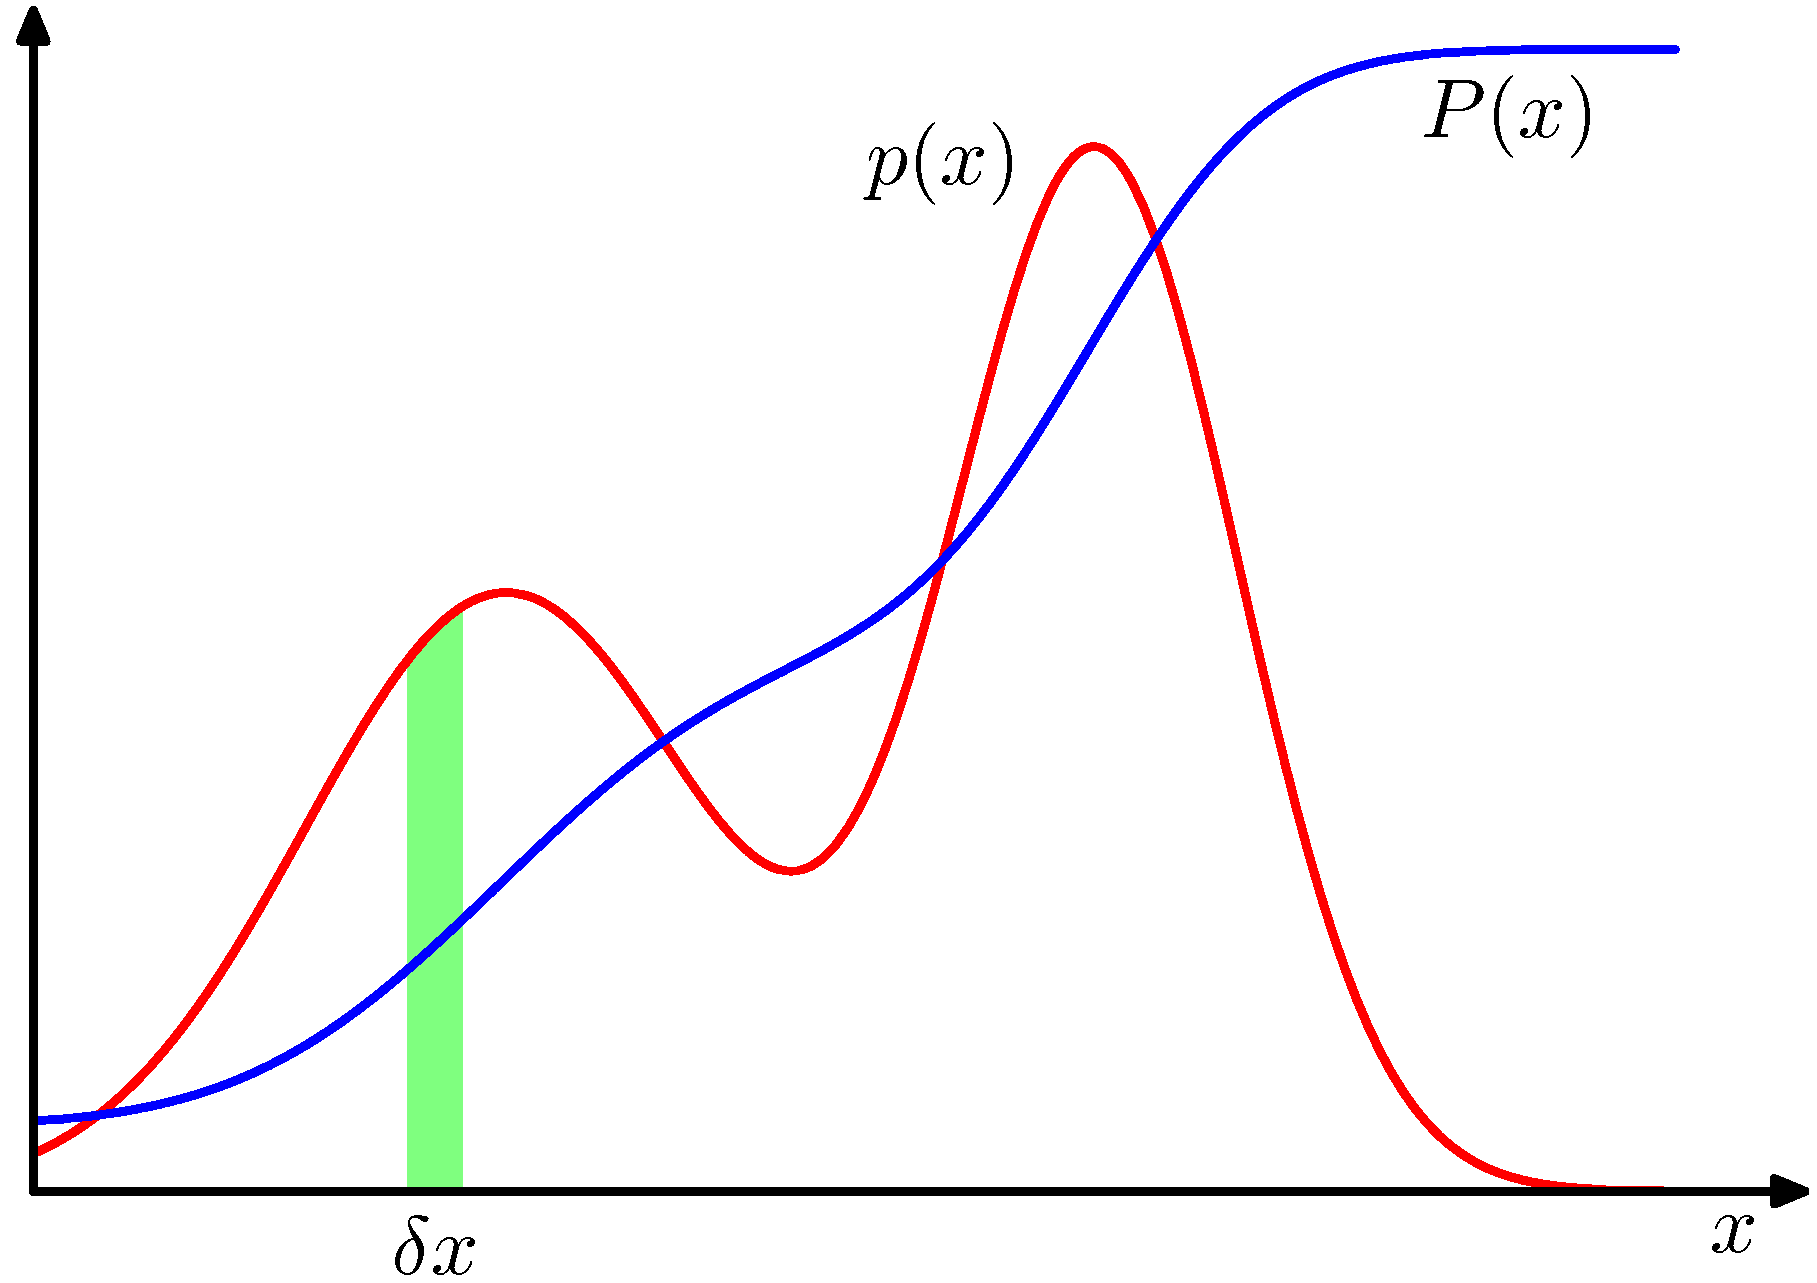
\includegraphics[scale=0.8]{Images/1-12.png}
		\captionsetup{font={small}}
		\caption{离散变量的概率可以扩展为连续变量$x$的概率密度$p(x)$,于是$x$的取值落在区间$(x,x+\delta x)$中的概率由$p(x)\delta x , \delta x \rightarrow 0$给出。概率密度可以被表示为累积分布函数(即分布函数,cumulative distribution function)的导数。} 
		\label{fig:1-12}	
	\end{figure}
	\\
	\indent 由于概率是非负的,而且$x$的值一定是在实轴范围内的,所以概率密度$p(x)$一定满足如下条件:
	\begin{align}
		p(x) &\geqslant 0 \\
		\int_{-\infty}^{+\infty}p(x)\ \mathrm{d}x &= 1
	\end{align}
	\indent 在变量的非线性变换下,由于雅可比因子(Jacobian factor),概率密度的变换与一般的函数不同。举例而言,假设有一个变量的变换$x=g(y)$,那么函数$f(x)$就变成了$\widetilde{f}(y)=f(g(y))$。接下来我们探讨一个概率密度函数$p_x(x)$,与它对应的是关于新变量的概率密度$p_y(y)$,这里使用了不同的下标来表示$p_x(x)$和$p_y(y)$是两个不同的概率密度。对于很小的$\delta x$,落在区间$(x,x+\delta x)$的结果将变换到$(y,y+\delta y)$中,且有$p_x(x)\delta x\approx p_y(y)\delta y$,于是
	\begin{equation}
		\begin{split}
			p_y(y)&=p_x(x)\left|\frac{\mathrm{d}x}{\mathrm{d}y}\right|\\
			&=p_x(x)(g(y))\left| g'(y) \right|
		\end{split}
	\end{equation}
	\indent 这个性质导致的结果之一是,概率密度的最大值取决于变量的选择。\color{red}\textbf{——习题1.4}\color{black}\\
	\indent $x$的取值落在区间$(-\infty,z)$中的概率由累积分布函数(cumulative distribution function)给出:
	\begin{equation}
		P(z)=\int_{-\infty}^{z}p(x)\ \mathrm{d}x
	\end{equation}
	\indent 很明显$P'(x)=p(x)$,如图1.12所示。\\
	\indent 如果有多个连续变量$x_1,...,x_D$,且将其合并记作向量$\mathbf{x}$,那么就可以定义一个联合概率密度$p(\mathbf{x})=p(x_1,...,x_D)$,这样$\mathbf{x}$落在一个无穷小体积$\delta \mathbf{x}$(其中包含了$\mathbf{x}$点)中的概率就可以表示为$p(\mathbf{x})\delta x$。多元概率密度一定满足:
	\begin{align}
		p(\mathbf{x}) &\geqslant 0 \\
		\int p(\mathbf{x})\  \mathrm{d} \mathbf{x} &= 1
	\end{align}
	\indent 其中的积分是在整个$\mathbf{x}$空间上的。此外我们还可以考虑离散变量和连续变量的联合概率分布。\\
	\indent 注意,如果$x$是一个离散变量,那么$p(x)$有时也被称为概率质量函数(probability mass function),因为可以看作是集中在可能的$x$取值处的“概率质量”的集合。\\
	\indent 加法规则、乘法规则和贝叶斯定理同样适用于概率密度,以及离散变量与连续变量联合的情况。举例而言,如果$x$和$y$是两个实值变量,那么加法规则和乘法规则有如下形式:
	\begin{align}
		p(x)&=\int p(x,y) \ \mathrm{d} y \\
		p(x,y)&=p(y|x)p(x)
	\end{align}
	正式地证明连续变量的加法规则和乘法规则(Feller,1966)需要使用大量测度论(measure theory)的内容,这远远超出了本书的范围。然而,通过将每个实变量划分成宽度为$\Delta$的区间,并考虑在这些区间上的离散概率分布,可以不太正式地看出这一做法的合理性。令$\Delta \rightarrow 0$,则可以将求和转化为积分,并给出一个确切的结果。
	}
	\subsection{期望与协方差}
	\textnormal{涉及到概率的最重要的运算之一就是寻找函数的加权平均值。函数$f(x)$在概率分布$p(x)$下的平均值被称为函数$f(x)$的期望(expectation),记作$\mathbb{E}[f]$。对于离散分布:
	\begin{equation}
		\mathbb{E}[f]=\sum_{x}^{} p(x)f(x)
	\end{equation}
	\indent 于是这个平均值由不同的$x$值对应的概率赋予了权值。对于连续变量的情况,期望是由对概率密度积分的形式表达的:
	\begin{equation}
		\mathbb{E}[f]=\int p(x)f(x)\ \mathrm{d}x
	\end{equation}
	\indent 无论是哪一种情况,如果从概率分布或概率密度中提取了有限的$N$个点,那么就可以利用这些点来估计期望:
	\begin{equation}
		\mathbb{E}[f] \approx \frac{1}{N}\sum_{n=1}^{N}f(x_n)
	\end{equation}
	\indent 我们将在第11章中对取样方法进行讨论时经常用到这个结论。在$N \rightarrow \infty$时,(1.35)中的估计将会变得很准确。\\
	\indent 有时候我们需要研究多元函数的期望,在这种情况下我们可以利用一个下标来表示求取的是哪个变量的均值,比如:
	\begin{equation}
		\mathbb{E}_x[f(x,y)]
	\end{equation}
	表示函数$f(x,y)$关于$x$的分布的平均值。需要注意的是,$\mathbb{E}_x[f(x,y)]$是一个关于$y$的函数。\\
	\indent 此外我们还可以研究关于条件分布的条件期望(conditional expectation)。即:
	\begin{equation}
		\mathbb{E}_x[f|y]=\sum_{x}^{}p(x|y)f(x)
	\end{equation}
	\indent 连续变量的情况与此类似。\\
	\indent 对于函数$f(x)$,其方差(variance)的定义为:
	\begin{equation}
		\mathrm{var} [f]=\mathbb{E}[(f(x)-\mathbb{E}[f(x)])^2]
	\end{equation}
	\indent 方差是一种对函数$f(x)$在其自身均值$\mathbb{E}[f(x)]$附近变化程度的度量。将平方项展开,我们可以看出函数的方差可以写成$f(x)$和$f(x)^2$的表达形式:\color{red}\textbf{——习题1.5}\color{black}
	\begin{equation}
		\mathrm{var}[f]=\mathbb{E}[f(x)^2]-\mathbb{E}[f(x)]^2
	\end{equation}
	\indent 特别地,我们可以计算变量$x$自身的方差,也就是:
	\begin{equation}
		\mathrm{var}[x]=\mathbb{E}[x^2]-\mathbb{E}[x]^2
	\end{equation}
	\indent 对于两个随机变量$x$和$y$,协方差(covariance)的定义为:
	\begin{equation}
		\begin{split}
			\mathrm{cov}[x,y] &= \mathbb{E}_{x,y}[\{x-\mathbb{E}[x]\}\{y-\mathbb{E}[y]\}] \\
							&= \mathbb{E}_{x,y}[xy]-\mathbb{E}[x]\mathbb{E}[y]
		\end{split}
	\end{equation}
	\indent 协方差表示了$x$和$y$一同变化的程度。如果$x$和$y$相互独立,那么其协方差就不存在了。\color{red}\textbf{——习题1.6}\color{black}\\
	\indent 对于两个由随机变量组成的向量$\mathbf{x}$和$\mathbf{y}$的情况,协方差是一个矩阵:
	\begin{equation}
		\begin{split}
			\mathrm{cov}[\mathbf{x,y}] &= \mathbb{E}_{\mathbf{x,y}}[\{\mathbf{x}-\mathbb{E}[\mathbf{x}]\}\{\mathbf{y}^\mathrm{T}-\mathbb{E}[\mathbf{y}^\mathrm{T}]\}] \\
			&= \mathbb{E}_{\mathbf{x,y}}[\mathbf{xy^\mathrm{T}}]-\mathbb{E}[\mathbf{x}]\mathbb{E}[\mathbf{y}^\mathrm{T}]
		\end{split}
	\end{equation}
	\indent 如果我们考虑的是$\mathbf{x}$的分量彼此之间的协方差,那么符号可以稍微简化一些,写成$\mathrm{cov}[\mathbf{x}] \equiv \mathrm{cov}[\mathbf{x,x}]$。}
	\subsection{贝叶斯概率}
	\textnormal{在本章节到目前为止的内容中,我们已经根据随机可重复事件的频率对概率有了一定的了解。我们将此称为概率的经典(classical)解释或频率(frequentist)解释。现在我们将转向更普遍的贝叶斯(Bayesian)观点。在贝叶斯观点中,概率是对不确定性的量化。\\
	\indent 对于一个不确定事件,如果这个事件是类似于月球是否曾经在独立的轨道上环绕太阳、北极冰盖是否会在本世纪末消失这样的事件,很明显它是不可重复的,所以这些事件的概率不能用类似前面水果箱子案例中的方法去描述。尽管如此,我们通常会有一些其他的想法,例如:北极的冰盖消融得有多快。如果我们能够得到一些新的证据,例如从新的地球观测卫星采集的新形式的诊断信息,我们就可以修正自己对冰消融速率的看法。对于此类事件的评估将进一步地影响我们的行为,例如我们正在努力减少温室气体的排放。在这种情况下,我们希望能够将不确定性量化,并根据新的证据来对不确定性进行精确的修正,以及能够在后续中采取最优的行动和决策。这些都可以通过概率的贝叶斯观点来实现,这是一个十分优美而且广泛应用的方法。\\
	\indent 尽管利用概率来表示不确定性并不是一个钦定的选择,但是如果我们希望做出合理清晰的推断,同时又尊重常识,那么它就是必不可少的。举例而言,Cox(1946)证明了如果利用数值表示置信度,那么一个包含了一系列常识属性的公理简单集合将唯一指向一个等价于概率论中加法规则和乘法规则的一系列操纵置信度的规则的集合。这是概率论可被视为带有不确定性的布尔逻辑的第一个证据(Jaynes, 2003)。还有很多作者提出了不确定性的度量应满足的其他属性或定理(Ramsey, 1931; Good, 1950; Savage, 1961; deFinetti, 1970; Lindley, 1982)。在这些情况下,根据概率论中的规则,这些数值结果都有比较精确的表现。所以将这些量看作是(贝叶斯观点的)概率就很正常了。\\
	\indent 同样地,在模式识别领域中,从更加普遍的视角来看待概率是很有帮助的。回想一下在1.1节中讨论的多项式曲线拟合的例子,应用概率的频率观点得到随机变量$t_n$似乎是很合理的。然而,我们希望针对模型参数$\mathbf{w}$能否做出合适选择的不确定性进行明确和量化。我们将看到,利用贝叶斯观点,我们可以使用概率论来描述$\mathbf{w}$这样的模型参数的不确定性,当然同样可以用于模型自身的选择上。\\
	\indent 贝叶斯定理现在有了新的意义。回想一下水果箱子的案例,我们看到了水果种类之后得到了相应的信息,并改变了“选择的箱子为红色”这一事件的概率。在此案例中,贝叶斯定理结合了观测结果(也就是水果种类)提供的新证据,将先验概率转换为后验概率。我们即将更清楚地看到,对多项式曲线拟合案例中的参数$\mathbf{w}$进行推断时,我们可以采用相似的方法。在得到观测结果之前,我们以先验概率分布$p(\mathbf{w})$的形式获取$\mathbf{w}$的假设。观测结果$\mathcal{D}=\{t_1,...,t_N\}$的影响通过条件概率$p(\mathcal{D}|\mathbf{w})$来表示,而且在1.2.5节中我们将会看到如何将它明确地表示出来。如此形式的贝叶斯定理:
	\begin{equation}
		p(\mathbf{w}|\mathcal{D})=\frac{p(\mathcal{D}|\mathbf{w})p(\mathbf{w})}{p(\mathcal{D})}
	\end{equation}
	将使我们能够以后验概率$p(\mathbf{w}|\mathcal{D})$的形式,在观测到$\mathcal{D}$\textbf{之后}估计$\mathbf{w}$的不确定性。\\
	\indent 贝叶斯定理等号右侧的$p(\mathcal{D}|\mathbf{w})$是对观测结果集合$\mathcal{D}$的估计,可以被视为一个关于参数向量$\mathbf{w}$的函数,称为似然函数(likelihood function)。它反映了对于不同的参数向量$\mathbf{w}$,不同的观测结果集合出现的可能性。需要注意的是,似然函数并非是关于$\mathbf{w}$的概率分布,对$\mathbf{w}$的积分也不一定等于1。\\
	\indent 在给出似然的定义之后,我们可以如此描述贝叶斯定理:
	\begin{equation}
		\mathrm{posterior \propto likelihood \times prior}
	\end{equation}
	\indent 其中所有的元素都可以看作是$\mathbf{w}$的函数。(1.43)中的分母为归一化常数,确保左侧的后验分布是概率密度且积分为1。事实上,将(1.43)两侧的式子对$\mathbf{w}$积分,我们就可以将贝叶斯定理中的分母表示为先验分布和似然函数的形式:
	\begin{equation}
		p(\mathcal{D})=\int p(\mathcal{D}|\mathbf{w})p(\mathbf{w})\ \mathrm{d}\mathbf{w}
	\end{equation}
	\indent 不论是在贝叶斯观点还是在频率观点中,似然函数$p(\mathcal{D}|\mathbf{w})$都扮演了核心的角色。然而,它在两种观点中的使用方式却完全不同。在频率观点中,$\mathbf{w}$被看作是一项确定的参数,其取值由某种形式的“估计”来确定,而估计的误差是根据数据集$\mathcal{D}$可能的分布来确定的。与之相反,贝叶斯观点认为数据集$\mathcal{D}$仅有一个,也就是观测到的那一个,而参数的不确定性是由$\mathbf{w}$的概率分布表示的。\\
	\indent 最大似然(maximum likelihood)是一种应用很广泛的频率估计,其中$\mathbf{w}$的值被设置为使得似然函数$p(\mathcal{D}|\mathbf{w})$取得最大值的数值,也就是说,在选择该$\mathbf{w}$时,该观测结果集合出现的概率达到最大。在机器学习的文献中,似然函数的负对数被称为误差函数(error function)。由于负对数是单调递减函数,所以似然的最大化等价于误差的最小化。\\
	\indent 定义频率误差的方法之一是bootstrap(解靴带/自助法,后者源自周志华编著的《机器学习》, Efron, 1979; Hastie et al., 2001),可根据如下方法生成多个数据集。假设我们有一个初始的数据集,其中包含了$N$个数据点$\mathbf{X}=\{\mathbf{x}_1,...,\mathbf{x}_N\}$。我们可以从$\textbf{X}$中随机抽取$N$个数据点,形成一个新的数据集$\textbf{X}_\textrm{B}$,其中抽取的点可以是重复的,所以$\textbf{X}$中的一些点会在$\textbf{X}_\textrm{B}$中重复出现,而有一些则根本不会出现。这一过程将重复$L$次,于是我们会得到$L$个大小为$N$的数据集,每个数据集都是各自独立地从初始数据集$X$中抽样出来的。参数估计的统计学准确度可以在后续中通过不同的自助数据集中预测结果的变化程度来进行估计。\\
	\indent 利用贝叶斯观点的优点之一是可以将先验内容自然地包含进来。举例而言,假设我们把一枚普通的硬币投掷三次,每次落地时都恰好是正面向上。那么对于正面向上这个事件,传统的最大似然估计给出的概率将是1,\color{red} \textbf{——第2.1节} \color{black}也就是说随便一扔就一定是正面向上!与之相反的是,贝叶斯观点将考虑一切合理的先验,得出的结论不会如此极端。\\
	\indent 频率学派和贝叶斯学派各有各的优点,两大学派之间也在无数的问题上存在无数的争论,尽管事实是,无论是频率学派还是贝叶斯学派,都是不能独立存在的。举个例子,对于贝叶斯学派的一大常见批判是,先验分布经常根据数学上计算的方便来选择,而非基于任何先验知识。甚至有人将“结论依赖于先验选择”这一主观本质都视为困难的来源。减少对先验的依赖是所谓无信息先验(noninformative priors)出现的动机之一。\color{red} \textbf{——第2.4.3节} \color{black}然而这样做的话,在不同的模型进行比较时就很困难,而且先验选项匮乏的贝叶斯方法可能会信心十足地给出一个很坏的结果。频率估计方法可以对这些问题有一定的规避,而且类似于交叉验证的方法,在模型比较等领域中仍然十分有用。\color{red} \textbf{——第1.3节} \color{black}\\
	\indent 本书非常强调贝叶斯观点,也体现了在过去的几年中,贝叶斯方法在实践中的重要性有了巨大的增长,同时也讨论了一些有用的频率域概念。\\
	\indent 尽管贝叶斯框架起源于18世纪,但贝叶斯方法的实际应用却在很长一段时间内受制于进行完整贝叶斯计算过程的困难,特别是在需要对完整的参数空间求边缘化(求和或积分)的情况下。而为了进行预测或进行不同模型之间的比较,完整参数空间上的计算又是必不可少的。类似马尔科夫链蒙特卡洛之类的采样方法的发展(第11章中将会讨论),以及计算机运行速度和内存容量的显著改进,使得贝叶斯方法在许多问题中得到了应用。蒙特卡洛方法非常灵活,可以应用于任何模型。然而它们的计算量很大,所以通常用于小规模的问题。\\
	\indent 最近,一些高效的确定性近似方案,类似变分贝叶斯和期望传播已经被提出(将在第10章中进行讨论)。这些方案提供了采样方法的补充和替代方法,并使得贝叶斯方法可以在大规模问题中得到应用(Blei et al., 2003)。
	}
	\subsection{高斯分布}
	\textnormal{我们将在整个第2章中研究各种概率分布及其关键性质。然而现在将最重要的连续变量概率分布之一——正态分布(normal distribution)或高斯分布(Gaussian distribution)引入会更方便一些。我们将在本章的剩余内容和其他大部分章节中广泛应用这一分布。\\
	\indent 对于一元实值变量$x$,高斯分布的定义为
	\begin{equation}
		\mathcal{N}(x|\mu,\sigma^2)=\frac{1}{(2\pi\sigma^2)^{1/2}}\exp\left\{-\frac{1}{2\sigma^2}(x-\mu)^2\right\}
	\end{equation}
	\indent 其中的两个参数,$\mu$为均值(mean),$\sigma^2$为方差(variance)。方差的平方根$\sigma$被称为标准差(standard deviation),方差的倒数$\beta =1/\sigma^2$被称为精度(precision)。我们很快将看到这些内容的意义。图1.13给出了高斯分布的图像。
	\begin{figure}[ht]
		\centering
		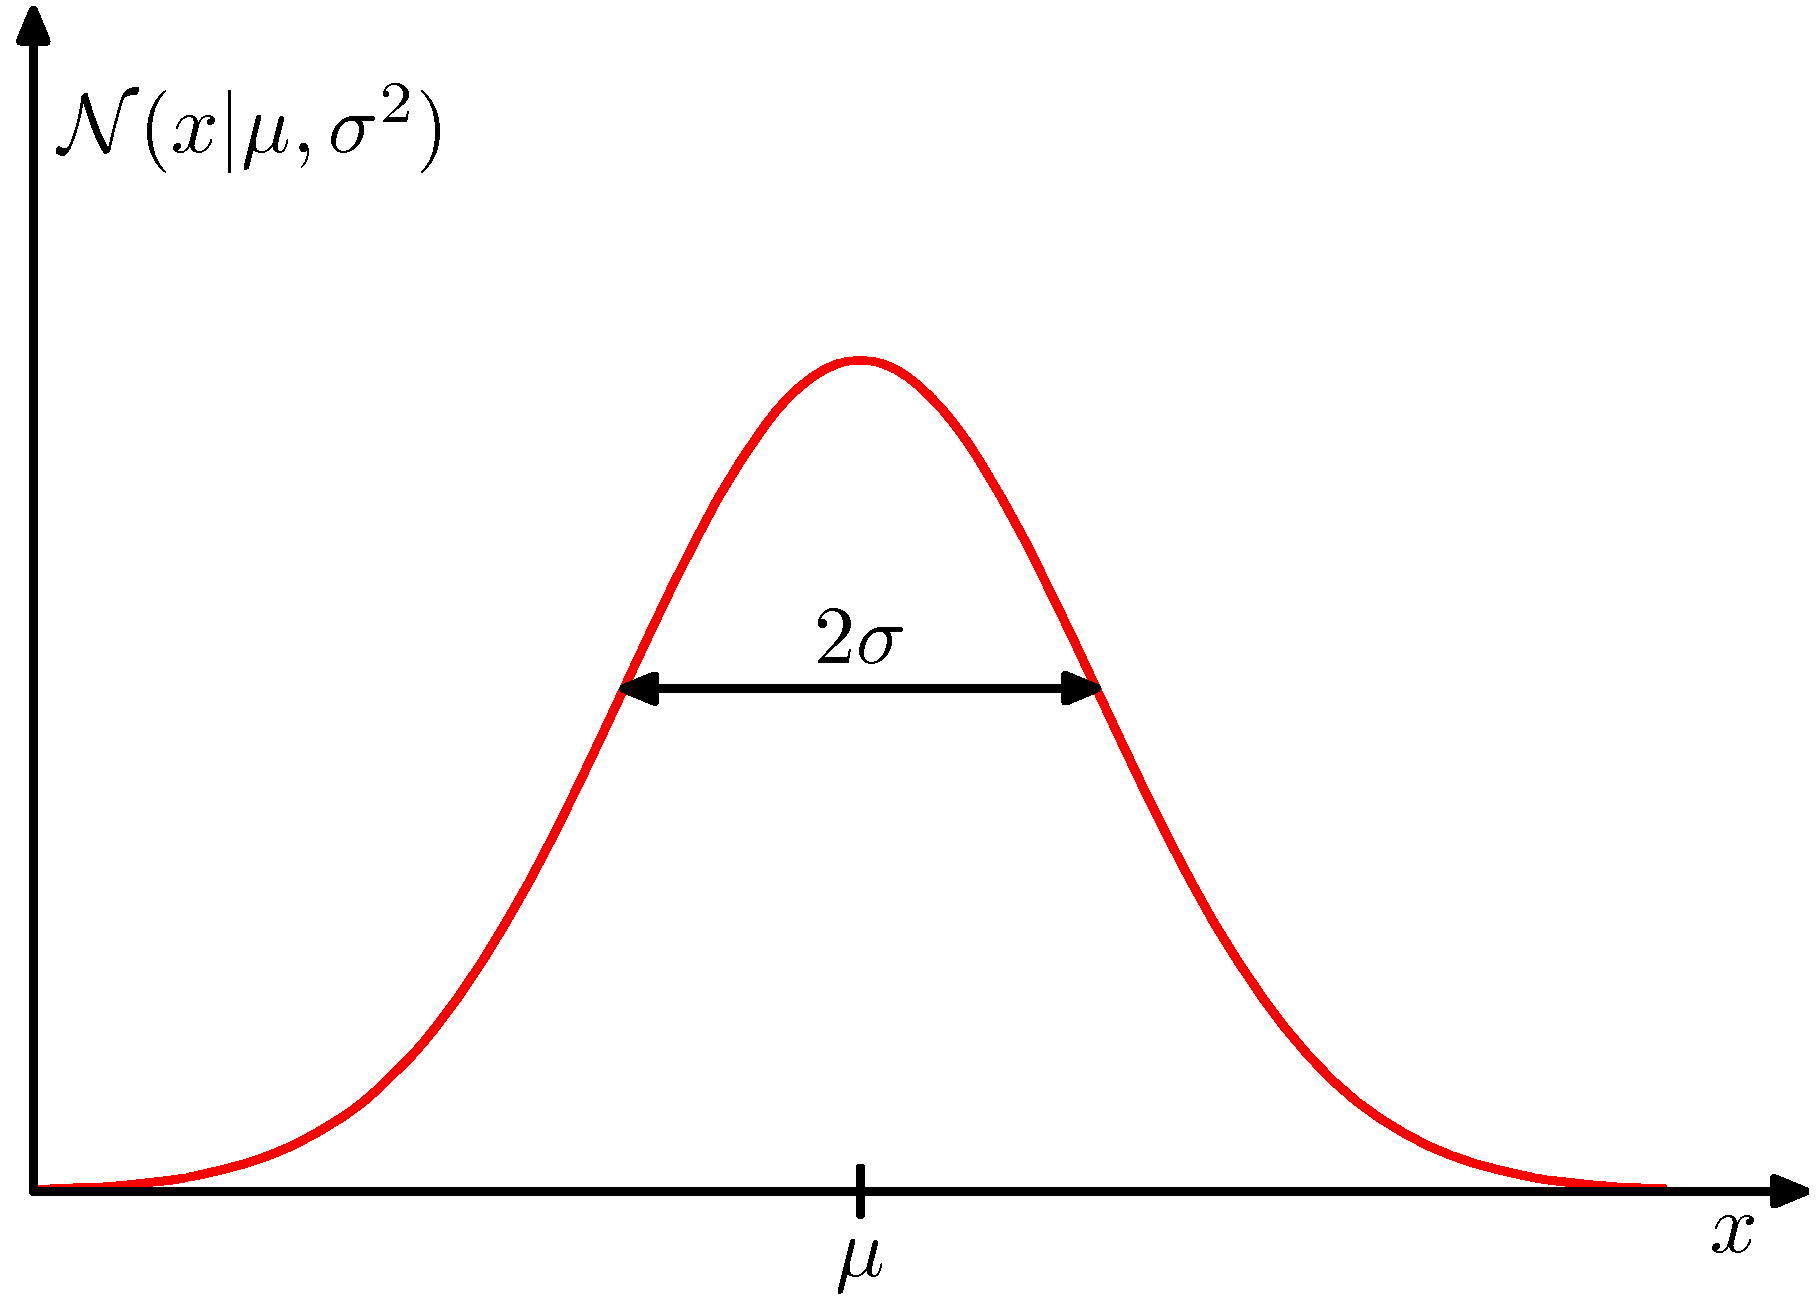
\includegraphics[scale=0.8]{Images/1-13.png}
		\captionsetup{font={small}}
		\caption{标出了均值$\mu$和标准差$\sigma$的高斯分布} 
		\label{fig:1-13}	
	\end{figure}
	\\
	\indent 从(1.46)的形式中我们可以看出,高斯分布满足
	\begin{equation}
		\mathcal{N}(x|\mu,\sigma^2)>0
	\end{equation}
	\indent 而且直接表明了高斯分布是归一化的。所以
	\begin{equation}
		\int_{-\infty}^{\infty}\mathcal{N}(x|\mu,\sigma^2)\ \mathrm{d}x = 1
	\end{equation}
	\indent 所以(1.46)满足概率密度的两项基本要求。\color{red} \textbf{——习题1.7} \color{black}\\
	\indent 我们很快就可以求出服从高斯分布的变量$x$的函数的期望。特别地,$x$的平均值为 \color{red} \textbf{\ \ ——习题1.8} \color{black}
	\begin{equation}
		\mathbb{E}[x]=\int_{-\infty}^{\infty}\mathcal{N}(x|\mu,\sigma^2)x\ \mathrm{d}x = \mu
	\end{equation}
	\indent 由于参数$\mu$表示$x$在该分布下的平均值,实际上就是期望。类似地,其二阶矩
	\begin{equation}
		\mathbb{E}[x^2]=\int_{-\infty}^{\infty}\mathcal{N}(x|\mu,\sigma^2)x^2\ \mathrm{d}x = \mu^2+\sigma^2
	\end{equation}
	\indent 根据(1.49)和(1.50),可以得到$x$的方差为
	\begin{equation}
		\mathrm{var}[x]=\mathbb{E}[x^2]-\mathbb{E}[x]^2=\sigma^2
	\end{equation}
	\indent 于是$\sigma^2$就是方差了。一个分布的最大值被称为模。对于高斯分布而言,其模是在均值处的函数值。\color{red} \textbf{——习题1.9} \color{black}\\
	\indent 我们还希望知道$D$维向量$\mathbf{x}$的高斯分布是怎样定义的。其定义如下:
	\begin{equation}
		\mathcal{N}(\mathbf{x}|\boldsymbol{\mu}, \boldsymbol{\Sigma})=\frac{1}{(2\pi)^{D/2}}\frac{1}{|\boldsymbol{\Sigma}|^{1/2}}\exp\left\{-\frac{1}{2}(\mathbf{x}-\boldsymbol{\mu})^\mathrm{T}\boldsymbol{\Sigma}^{-1}(\mathbf{x}-\boldsymbol{\mu})\right\}
	\end{equation}
	\indent 其中的$D$维向量$\boldsymbol{\mu}$为均值,$D \times D$维矩阵$\boldsymbol{\Sigma}$为协方差,$|\boldsymbol{\Sigma}|$表示$\boldsymbol{\Sigma}$的行列式。我们将在本章节中稍微应用一些多元高斯分布,详细的内容将在第2.3节中学习。\\
	\indent 现在假设我们有一个观测数据集$\boldsymbol{\mathsf{x}}=(x_1,...,x_N)^\mathrm{T}$,表示$N$个对于标量变量$x$的观测。注意,这里我们使用了$\boldsymbol{\mathsf{x}}$这样的符号与$\mathbf{x}$区分开,后者表示对于向量变量$(x_1,...,x_D)^\mathrm{T}$的单一观测。我们假设数据集中所有的观测都是从一个$\mu$和$\sigma^2$都未知的高斯分布中相互独立地抽取出来的,并希望根据这个数据集确定这两个参数。一组从相同的分布中相互独立取出的数据点是独立同分布(independent and identically distributed)的,简称“i.i.d.”。我们已经知道两个独立事件的联合概率是由事件各自的边缘概率求取乘积得到的。由于数据集$\boldsymbol{\mathsf{x}}$是独立同分布的,所以我们可以写出给定$\mu$和$\sigma^2$的条件下该观测出现的概率:
	\begin{equation}
		p(\boldsymbol{\mathsf{x}}|\mu,\sigma^2) = \prod_{n=1}^{N}\mathcal{N}(x_n|\mu,\sigma^2)
	\end{equation}
	\indent 将其视为$\mu$和$\sigma^2$的函数,它就变成了一个高斯分布的似然函数,如图1.14所示。
	\begin{figure}[ht]
		\centering
		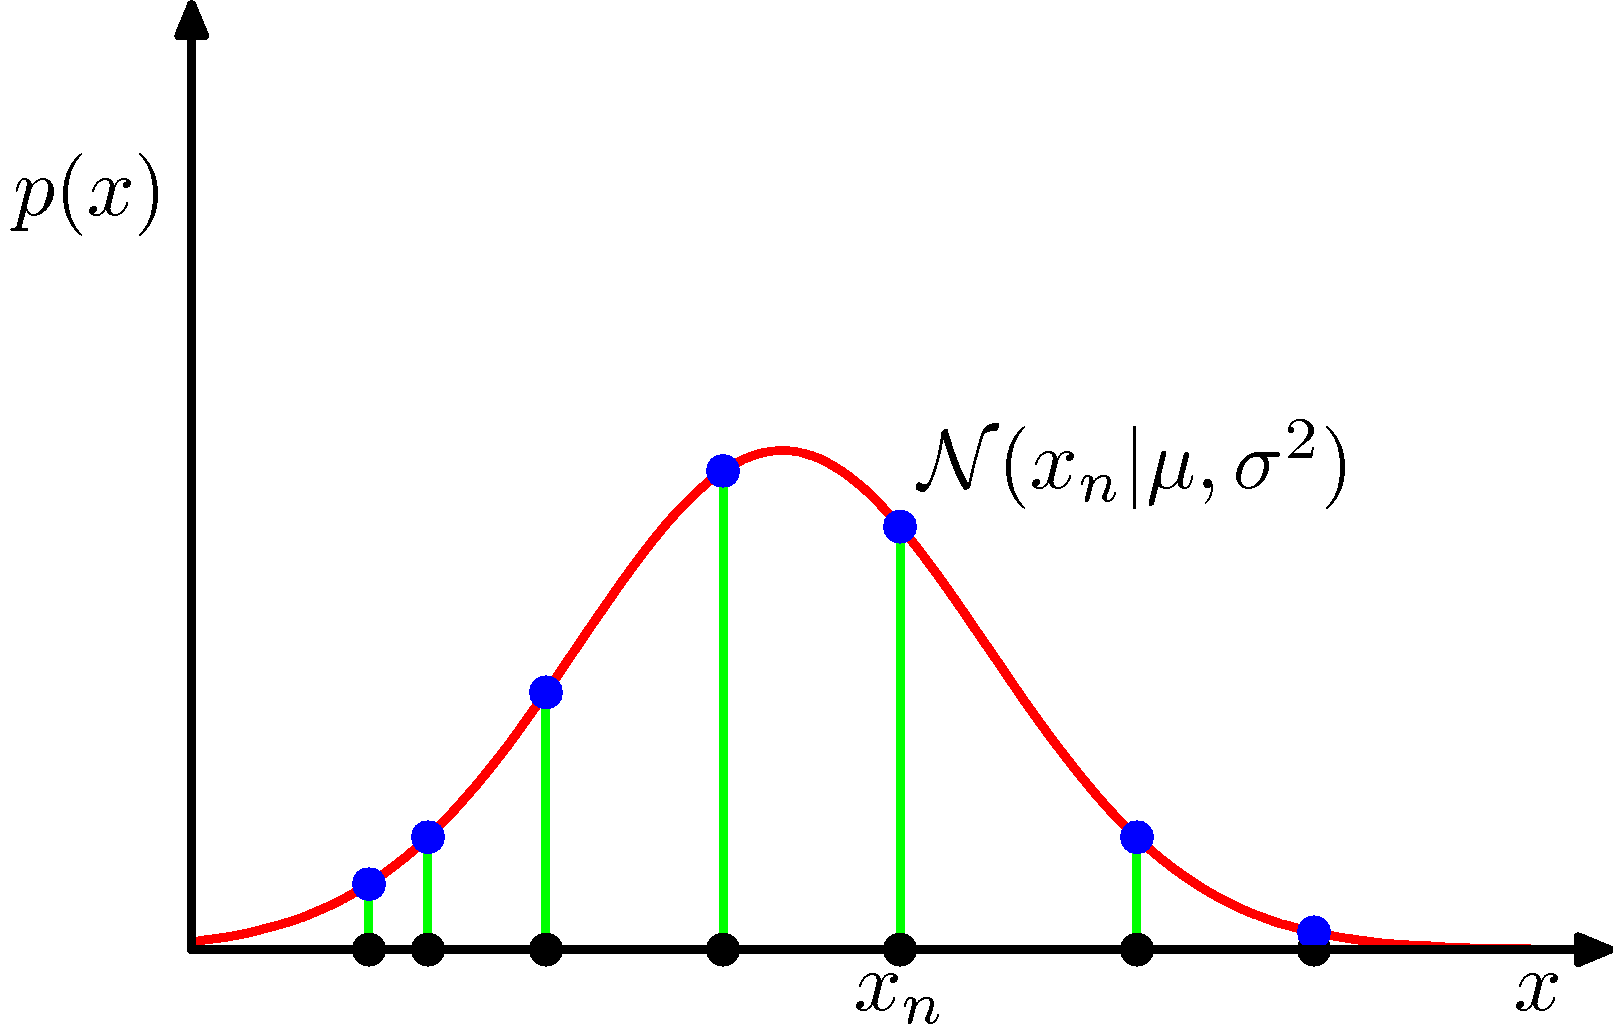
\includegraphics[scale=0.8]{Images/1-14.png}
		\captionsetup{font={small}}
		\caption{高斯分布的似然函数,即图中的红色曲线。黑点表示数据集中的值$\left\{x_n\right\}$,(1.53)中给出的似然函数对应的是图中蓝点的乘积。似然函数最大化的过程也包含了均值和方差的调整,从而使该乘积达到最大值。}
		\label{fig:1-14}	
	\end{figure}
	\\
	\indent 利用观测结果集合进行概率分布中参数的确定,一个常见的办法是找出使得似然函数达到最大值的参数值。这看起来似乎挺奇怪,因为从前面所学的概率论来看,根据给定的数据去求参数的概率最大值似乎更加自然一些,而非根据给定的参数去求数据的概率最大值。事实上,这两个标准是相关的,我们将在后文中结合曲线拟合的例子来讨论这个问题。\color{red} \textbf{——第1.2.5节} \color{black}\\
	\indent 不过,现在我们还是利用(1.53)中似然函数的最大化来确定高斯分布的未知参数$\mu$和$\sigma^2$。在实际应用中,对似然函数的对数求最大值要更方便一些。因为对数函数是单调递增函数,对数函数的最大化与函数自身求取最大化是等价的。求对数不仅简化了随后的分析,而且还利于数值计算,因为大量较小概率的乘积会使计算机的数值精度下降,而对概率对数求和就不会有这样的问题。根据(1.46)和(1.53),对数似然函数可以写成:
	\begin{equation}
		\ln p(\boldsymbol{\mathsf{x}}|\mu,\sigma^2)=-\frac{1}{2\sigma^2}\sum_{n=1}^{N}(x_n-\mu)^2-\frac{N}{2}\ln \sigma^2-\frac{N}{2}\ln(2\pi)
	\end{equation}
	\indent 求(1.54)关于$\mu$的最大值,可以得到最大似然解\color{red} \textbf{\ \ ——习题1.11} \color{black}
	\begin{equation}
		\mu_{\mathrm{ML}}=\frac{1}{N}\sum_{n=1}^{N}x_n
	\end{equation}
	\indent 也就是样本均值(sample mean),即观测值$\left\{x_n\right\}$的均值。类似地,求(1.54)关于$\sigma^2$的最大值,可以得到:
	\begin{equation}
		\sigma_{\mathrm{ML}}^2=\frac{1}{N}\sum_{n=1}^{N}(x_n-\mu_{\mathrm{ML}})^2
	\end{equation}
	\indent 也就是基于样本均值$\mu_{\mathrm{ML}}$的样本方差(sample variance)。需要注意的是,我们要对(1.54)关于$\mu$和$\sigma^2$进行最大化,但对于高斯分布而言,$\mu$的解和$\sigma^2$无关,所以可以先估计(1.55)再利用结果估计(1.56)。\\
	\indent 在本章稍后的内容和以后的章节中,我们将指明最大似然方法有很严重的局限性。现在我们先通过一元高斯分布的最大似然参数解简单阐述一下这个问题。特别地,我们将证明最大似然方法非常整齐划一地低估了分布的方差。这种现象被称为偏移(bias),与多项式曲线拟合问题中的过拟合问题有关。首先注意到,最大似然解$\mu_{\mathrm{ML}}$和$\sigma_{\mathrm{ML}}^2$都是数据集中的值$x_1,...,x_N$的函数。考虑到这两个值基于数据集的期望,而数据集是来自参数为$\mu$和$\sigma^2$的高斯分布的。所以可以直接写出:\color{red} \textbf{——第1.1节, 习题1.12} \color{black}
	\begin{align}
		\mathbb{E}[\mu_{\mathrm{ML}}] &=\mu \\
		\mathbb{E}[\sigma_{\mathrm{ML}}^2]&=\left(\frac{N-1}{N}\right)\sigma^2
	\end{align}
	\indent 于是最大似然估计的均值可以确定正确的期望,但将使估计的方差带有一个系数$(N-1)/N$,所以会比真实值偏低。这个结果背后的原因如图1.15所示。
	\begin{figure}[ht]
		\centering
		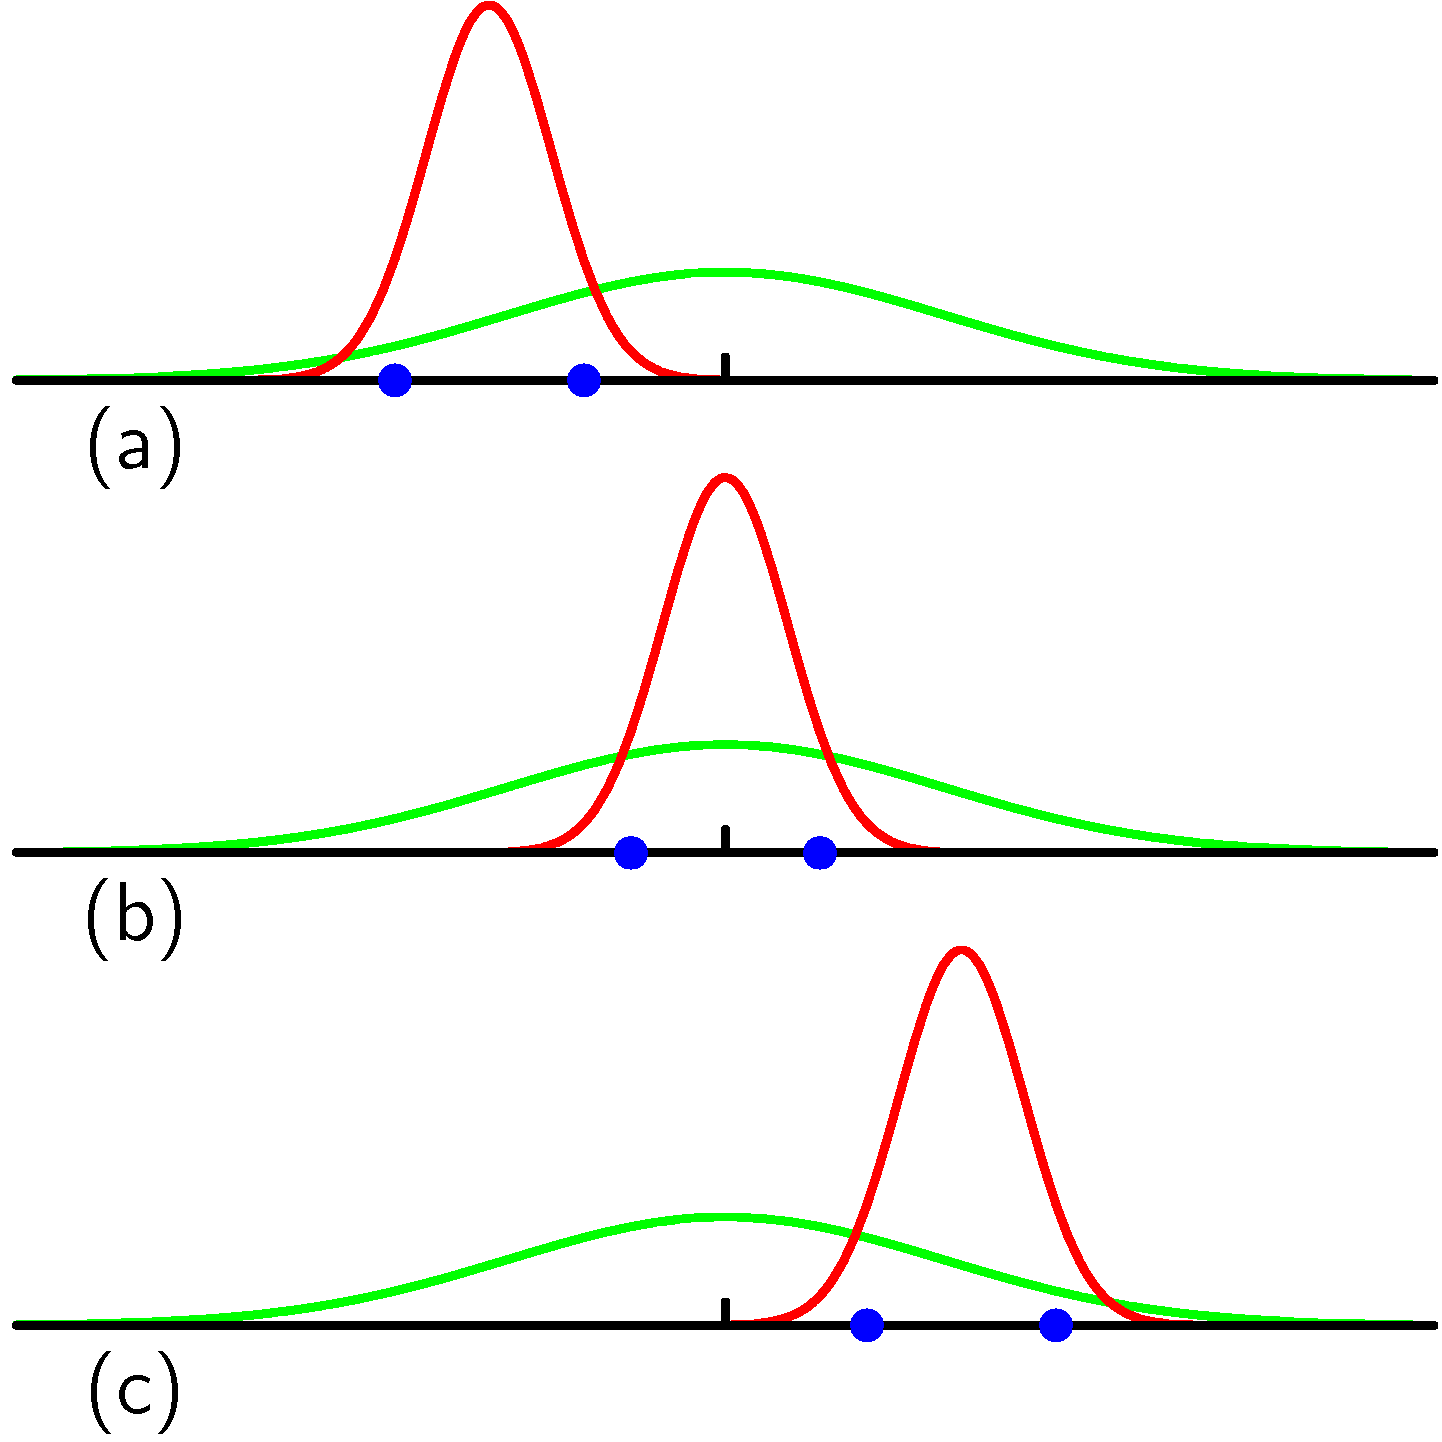
\includegraphics[scale=0.8]{Images/1-15.png}
		\captionsetup{font={small}}
		\caption{在利用最大似然估计确定高斯分布的方差时产生偏移的说明。其中绿色的曲线表示产生数据集的真实高斯分布,三条红色曲线表示基于三个不同的数据集得到的高斯分布拟合结果,每个数据集包含两个数据点,在图中用蓝色的点表示,根据(1.55)和(1.56)给出的结论进行拟合。对三个数据集求平均数,可以看出均值是正确的,但方差被低估了,因为它根据样本均值确定,而非真实的均值。}
		\label{fig:1-15}
	\end{figure}
	\\
	\indent 根据(1.58),下面对于方差参数的估计才是无偏的:
	\begin{equation}
		\widetilde{\sigma}^2 = \frac{N}{N-1}\sigma_{\mathrm{ML}}^2 = \frac{1}{N-1}\sum_{n=1}^{N}(x_n-\mu_{\mathrm{ML}})^2
	\end{equation}
	\indent 在第10.1.3节中我们将看到在应用贝叶斯方法时,这个结果会自然地形成出来。\\
	\indent 需要注意的是,随着数据点数量$N$的增加,最大似然解的偏移将显得越来越不显著,而且当$N \rightarrow \infty$时,方差的最大似然解就是产生数据的分布的方差。在实践中,除非$N$比较小,否则偏移都不会很严重。但是,在本书中,我们对具有很多参数的复杂模型更感兴趣,在这种模型中,最大似然的偏移问题将会比较严重。实际上,我们即将看到,最大似然的偏移问题正是之前讨论的多项式曲线拟合问题中过拟合问题的根源。
	}
	\subsection{重返曲线拟合问题}
	\textnormal{我们已经见证了多项式曲线拟合问题可以用误差最小化的形式表达出来。现在我们返回到曲线拟合的例子中,并通过概率的观点来审视它,从而得到一些关于误差函数和正则化的见解,并将我们引入到完整的贝叶斯方法中。\color{red} \textbf{——第1.1节} \color{black}\\
	\indent 曲线拟合问题的目标,是基于包含有$N$组输入变量$\boldsymbol{\mathsf{x}}=(x_1,...,x_N)^{\mathrm{T}}$及其对应的目标变量$\boldsymbol{\mathsf{t}}=(t_1,...,t_N)^{\mathrm{T}}$的训练数据集,当输入变量$x$有新的取值时,对目标变量$t$进行预测。我们可以利用概率分布,表示目标变量取值的不确定性。对此,我们假设在给定$x$的情况下,对应的$t$服从均值为$y(x,\mathbf{w})$的高斯分布,其中的$y(x,\mathbf{w})$为(1.1)中多项式曲线给出的函数值。于是我们就有:
	\begin{equation}
		p(t|x,\mathbf{w},\beta)=\mathcal{N}(t|y(x,\mathbf{w}),\beta^{-1})
	\end{equation}
	\indent 其中,为了与后面章节中的符号统一,我们定义了一个精确度参数$\beta$,表示该分布的逆方差。图1.16给出了具体的说明。
	\begin{figure}[ht]
		\centering
		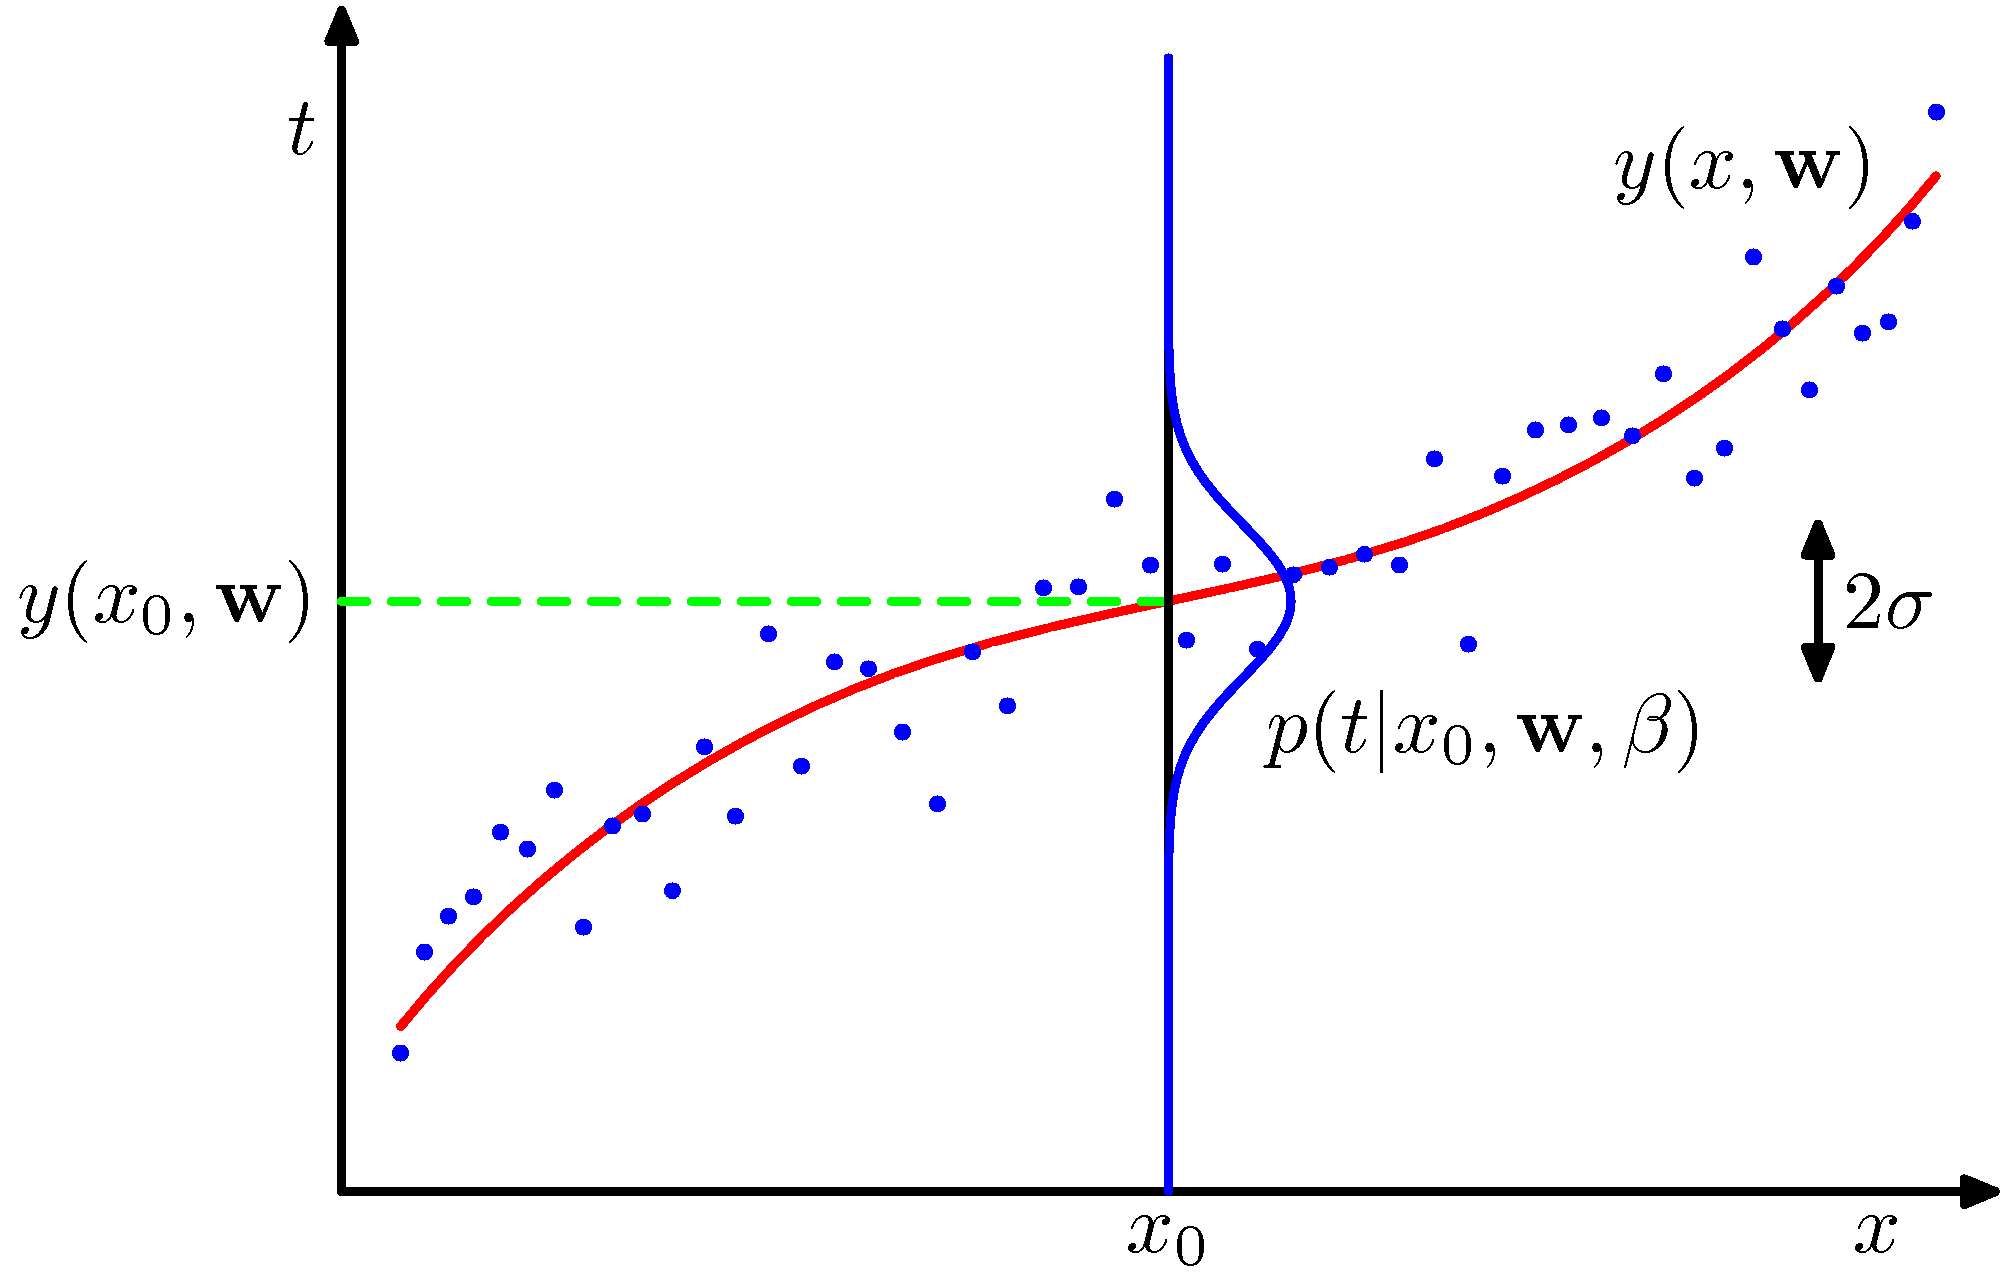
\includegraphics[scale=0.8]{Images/1-16.png}
		\captionsetup{font={small}}
		\caption{(1.60)中给定$x$的情况下$t$的高斯分布。其均值由多项式函数$y(x,\mathbf{w})$给出,$\beta$为与方差相关的精确度参数,$\beta^{-1}=\sigma^2$。}
		\label{fig:1-16}
	\end{figure}
	\\
	\indent 现在基于训练数据$\left\{\boldsymbol{\mathsf{x}},\boldsymbol{\mathsf{t}}\right\}$,利用最大似然来确定未知参数$\mathbf{w}$和$\beta$。如果假设数据是从(1.60)中的分布中相互独立地提取出来的,那么似然函数就可以写成:
	\begin{equation}
		p(\boldsymbol{\mathsf{t}}|\boldsymbol{\mathsf{x}},\mathbf{w},\beta) = \prod_{n=1}^{N}\mathcal{N}(t_n|y(x_n,\mathbf{w}),\beta^{-1})
	\end{equation}
	\indent 正如我们早些时候对于高斯分布的处理一样,对似然函数的对数求最大值要更加方便。根据(1.46)给出的高斯函数的形式,可以写出对数似然函数:
	\begin{equation}
		\ln p(\boldsymbol{\mathsf{t}}|\boldsymbol{\mathsf{x}},\mathbf{w},\beta)=-\frac{\beta}{2}\sum_{n=1}^{N}\left\{y(x_n,\mathbf{w})-t_n\right\}^2 + \frac{N}{2}\ln \beta - \frac{N}{2}\ln(2\pi)
	\end{equation}
	\indent 首先确定多项式系数的最大似然解,用$\mathbf{w}_\mathrm{ML}$来表示。它们是通过对(1.62)关于$\mathbf{w}$进行最大化得到的。所以我们可以省略(1.62)等号右边的后两项,因为这两项与$\mathbf{w}$无关。同时,我们注意到在对数似然函数前面乘一个正数并不影响使得函数取得最大值的$\mathbf{w}$的取值,所以可以用1/2替换系数$\beta/2$。最后,求取对数似然函数的最大值,等价于求取负对数似然函数的最小值。于是对确定的$\mathbf{w}$而言,将似然函数最大化与将(1.2)中定义的平方和误差函数最小化是等价的。因此,平方和误差函数作为在高斯噪声下的最大似然的结果出现了。\\
	\indent 我们同样可以使用最大似然来确定高斯条件分布中的精确度参数$\beta$。关于$\beta$对(1.62)求最大化:
	\begin{equation}
		\frac{1}{\beta_\mathrm{ML}} = \frac{1}{N}\sum_{n=1}^{N}\left\{y(x_n,\mathbf{w}_\mathrm{ML})-t_n\right\}^2
	\end{equation}
	\indent 我们仍然首先确定控制均值的参数向量$\mathbf{w}_\mathrm{ML}$,然后使用它来求取精确度$\beta_\mathrm{ML}$,和此前处理简单高斯分布的情况一样。\color{red} \textbf{——第1.2.4节} \color{black}\\
	\indent 在确定了参数$\mathbf{w}$和$\beta$之后,就可以对新的$x$值做预测了。由于我们有了一个概率模型,所以预测不是以单一点估计的形式,而是由$t$的预测分布(predictive distribution)的形式给出的,而且这个分布是通过将最大似然参数代入(1.60)中得到的:
	\begin{equation}
		p(t|x,\mathbf{w}_\mathrm{ML},\beta_\mathrm{ML})=\mathcal{N}(t|y(x,\mathbf{w}_\mathrm{ML}),\beta_\mathrm{ML}^{-1})
	\end{equation}
	\indent 现在我们向贝叶斯方法更进一步,引入多项式系数$\mathbf{w}$的先验分布。简单起见,考虑如下形式的高斯分布:
	\begin{equation}
		p(\mathbf{w}|\alpha)=\mathcal{N}(\mathbf{w}|\mathbf{0},\alpha^{-1}\mathbf{I})=\left(\frac{\alpha}{2\pi}\right)^{(M+1)/2}\exp\left\{-\frac{\alpha}{2}\mathbf{w}^\mathrm{T}\mathbf{w}\right\}
	\end{equation}
	\indent 其中的$\alpha$是分布的精确度,$M+1$是$M$阶多项式对应的向量$\mathbf{w}$中元素的总数。类似$\alpha$这样的控制分布模型参数的变量称为超参数(hyperparameters)。利用贝叶斯定理,$\mathbf{w}$的后验分布与先验分布和似然函数的乘积成正比:
	\begin{equation}
		p(\mathbf{w}|\boldsymbol{\mathsf{x}},\boldsymbol{\mathsf{t}},\alpha,\beta) \propto p(\boldsymbol{\mathsf{t}}|\boldsymbol{\mathsf{x}},\mathbf{w},\beta)p(\mathbf{w}|\alpha)
	\end{equation}
	\indent 现在可以基于给定数据求取最可能的$\mathbf{w}$值,换句话说,也就是通过后验分布最大化来确定$\mathbf{w}$了。这个方法称为最大后验估计(maximum posterior),简称MAP方法。对(1.66)取负对数,并结合(1.62)和(1.65),我们发现后验的最大值是由以下公式的最小值给出的:
	\begin{equation}
		\frac{\beta}{2}\sum_{n=1}^{N}\left\{y(x_n,\mathbf{w})-t_n\right\}^2 + \frac{\alpha}{2}\mathbf{w}^\mathrm{T}\mathbf{w}
	\end{equation}
	\indent 于是,我们发现后验分布最大化等价于(1.4)中的正则化平方和误差函数最小化,其正则化参数由$\lambda = \alpha/\beta$来确定。
	}
	\subsection{曲线拟合的贝叶斯方法}
	\textnormal{尽管我们已经将先验分布$p(\mathbf{w}|\alpha)$包含了进来,但对于$\mathbf{w}$的估计仍然是点估计,不算是一个贝叶斯方法。在一个完整的贝叶斯方法中,我们应该连贯地应用概率的加法和乘法规则,正如我们即将要看到的一样,这需要我们对所有的$\mathbf{w}$积分。这样的边缘化是模式识别贝叶斯方法的核心。\\
	\indent 在曲线拟合问题中,我们有训练数据$\boldsymbol{\mathsf{x}}$和$\boldsymbol{\mathsf{t}}$和一个新的测试点$x$,我们的目标是预测$t$的值。所以我们希望估计一个预测分布$p(t|x,\boldsymbol{\mathsf{x}},\boldsymbol{\mathsf{t}})$。现在假设参数$\alpha$和$\beta$是固定且已知的(在后续的章节中我们将讨论如何从贝叶斯设定中推断这两个参数)。\\
	\indent 简单来说,贝叶斯方法就是从始至终地运用概率的加法规则和乘法规则,这使得预测分布可以写成如下形式:
	\begin{equation}
		p(t|x,\boldsymbol{\mathsf{x}},\boldsymbol{\mathsf{t}})=\int p(t|x,\mathbf{w})p(\mathbf{w}|\boldsymbol{\mathsf{x}},\boldsymbol{\mathsf{t}})\ \mathrm{d}\mathbf{w}
	\end{equation}
	\indent 其中的$p(t|x,\mathbf{w})$是由(1.60)确定的,同时为了简化,省略了对$\alpha$和$\beta$的依赖。$p(\mathbf{w}|\boldsymbol{\mathsf{x}},\boldsymbol{\mathsf{t}})$是参数的后验分布,可以通过将(1.66)等号右边的式子正则化来得到。我们将在第3.3节中看到,对于类似曲线拟合这样的问题,其后验分布是一个高斯分布,而且可以估计出其解析形式。类似地,(1.68)中的积分同样可以解析表达,于是预测分布可以写成如下形式的高斯分布:
	\begin{equation}
		p(t|x,\boldsymbol{\mathsf{x}},\boldsymbol{\mathsf{t}})=\mathcal{N}(t|m(x),s^2(x))
	\end{equation}
	\indent 其中的均值和方差为:
	\begin{align}
		m(x)&=\beta \phi(x)^\mathrm{T}\mathbf{S}\sum_{n=1}^{N}\phi(x_n)t_n \\
		s^2(x) &= \beta^{-1} + \phi(x)^\mathrm{T}\mathbf{S}\phi(x)
	\end{align}
	\indent 其中的矩阵$\mathbf{S}$为:
	\begin{equation}
		\mathbf{S}^{-1}=\alpha\mathbf{I}+\beta\sum_{n=1}^{N}\phi(x_n)\phi(x_n)^\mathrm{T}
	\end{equation}
	\indent 其中的$\mathbf{I}$为单位矩阵,$\phi(x)$为向量,其元素$\phi_i(x)=x^i,i=0,...,M$。\\
	\indent 由(1.69)可见,预测分布的均值和方差都依赖于$x$。(1.71)中的第一项表示的是由于噪声影响,在估计目标变量$t$时形成的不确定度,此时已经可以用(1.64)中最大似然预测分布的$\beta_{\mathrm{ML}}^{-1}$来表示。然而,公式的第二项来自参数$\mathbf{w}$的不确定度,是贝叶斯处理的结果。关于正弦曲线回归问题的说明如图1.17所示。
	\begin{figure}[H]
		\centering
		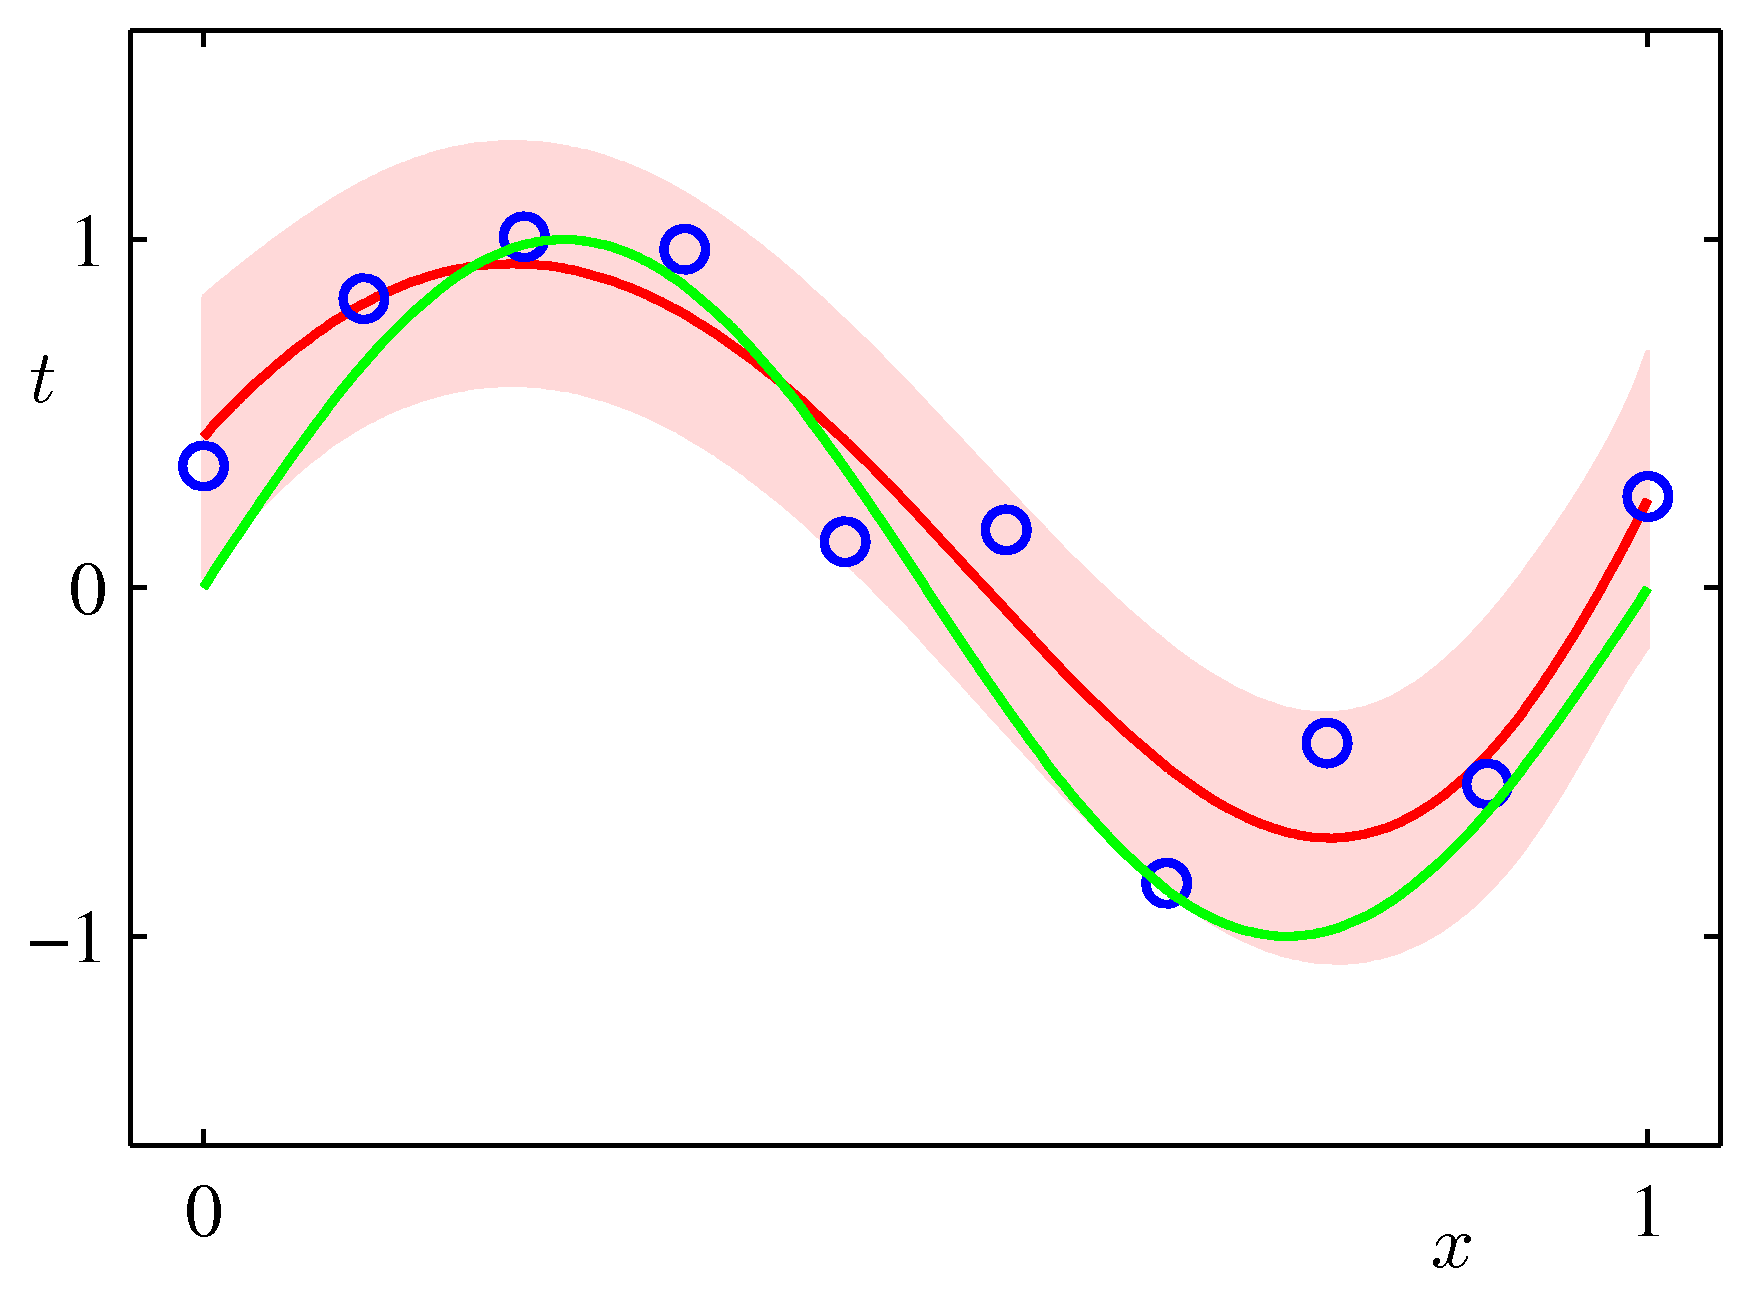
\includegraphics[scale=0.8]{Images/1-17.png}
		\captionsetup{font={small}}
		\caption{利用$M=9$的多项式,利用贝叶斯处理得到的多项式曲线拟合结果,其中,参数$\alpha = 5 \times 10^{-3}$,$\beta = 11.1$(对应于已知的噪声方差),红色的曲线表示预测分布的均值,红色的区域表示平均值附近$\pm1$标准差的区域。}
		\label{fig:1-17}
	\end{figure}
	}
	\section{模型选择}
	\noindent{\color{red} \rule[10pt]{\textwidth}{0.1em}}
	\textnormal{
	\indent 在我们利用最小二乘进行多项式曲线拟合的例子中,可以看到会有一个最优阶数的多项式,使得模型的泛化性能达到最佳。多项式的阶数控制着模型中自由参数的个数,所以也控制着模型的复杂度。在正则化最小二乘中,正则化系数$\lambda$同样也控制着模型的复杂度。而对于更加复杂的模型,例如混合分布和神经网络,更是可能存在更多的控制模型复杂度的参数。在实际应用中,我们需要确定这些参数,从而使得模型对于新的数据具有最优的预测性能。此外,除了对一个给定模型寻求合适的复杂度参数,我们还希望同时考虑一系列不同类型的模型,以便为特定的应用找到最佳的模型。\\
	\indent 我们已经在最大似然方法中看到,由于过拟合问题的存在,模型在训练集上的性能并不能真实反映出其在未知数据上的预测性能。如果数据充足,那么一种方法是使用一些现有的数据训练一系列的模型,或者给出某个复杂度参数下多组参数的模型,然后在独立出来的数据(有时称为验证(validation)集)上进行比较,并选择预测性能最优的那一个。如果使用一个大小有限的数据集在模型设计时进行多次的迭代,就可能出现对验证数据过拟合的现象,所以有必要提前把第三个数据集——测试集(test set)独立取出,最后再用于评估所选模型的性能。\\
	\indent 然而在很多应用中,用于训练和测试的数据会不太够用。在这种情形下,还想要构建好的模型,我们就希望能够用尽可能多的数据去训练。然而,如果验证集太小,那么模型对于预测性能的估计就是附带有噪声的。对这种进退两难的情况,一种解法是利用交叉验证(cross-validation),如图1.18所示。这种方法使得$(S-1)/S$的数据可以用于训练,同时还可以让所有数据都可以用于评估模型性能。当数据特别稀缺时,留一法(leave-one-out)是比较合适的,也就是使$S$等于数据点总数$N$。
	\begin{figure}[ht]
		\centering
		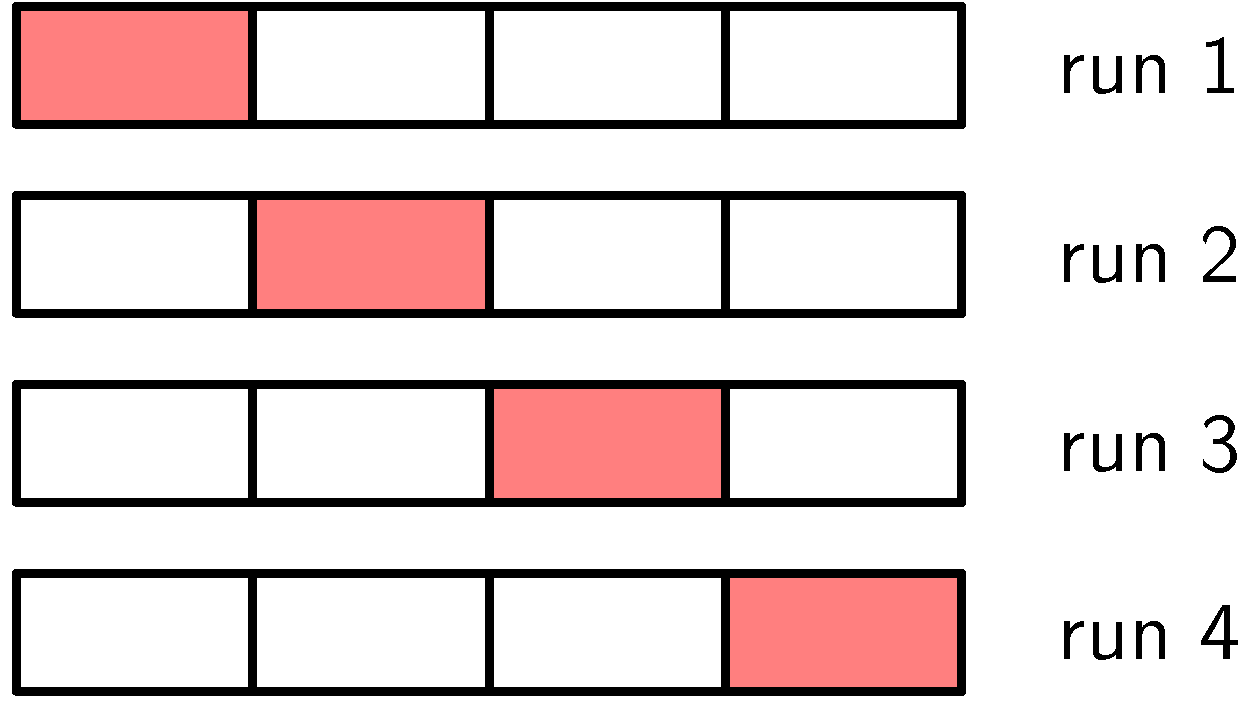
\includegraphics[scale=0.8]{Images/1-18.png}
		\captionsetup{font={small}}
		\caption{以$S=4$为例的$S$重交叉验证,将可用数据划分为$S$组(最简单的办法是平均分配,每组的数据数量一样)。于是$S-1$组的数据可以用于训练模型,剩下的组用于评估。然后对于留出组(红色方块)的所有$S$种可能的情况重复这个过程,最后对$S$次实验中的性能得分取平均数。}
		\label{fig:1-18}
	\end{figure}
	\\
	\indent 交叉验证的一个主要缺点是使训练的次数增加了$S$倍,这对于本身计算量就很大的模型来说就是很有问题的。类似于交叉验证这样将数据拆分来验证性能的做法还有一个问题是,对于一个模型可能会有多个复杂度参数(举例来说,可能会有好几个正则化参数)。在最坏的情况下,寻找这些参数的组合可能会需要参数数量指数倍的训练。很明显,我们需要更好的办法。在理想情况下,这个办法应该仅依赖于训练数据,而且允许在单个的训练中比较多个具有不同超参数和类型的模型。因此我们需要找到一种性能指标,它应该仅依赖于训练数据,而且不会因过拟合而造成偏差。\\
	\indent 历史上已经提出了很多个“信息标准”,试图通过惩罚项来校正最大似然的偏差,以弥补复杂模型的过拟合问题。例如Akaike信息标准,即AIC(Akaike, 1974),会选择如下值取得最大的模型:
	\begin{equation}
		\ln p(\mathcal{D}|\mathbf{w}_{\mathrm{ML}}) -M
	\end{equation}
	\indent 其中的$p(\mathcal{D}|\mathbf{w}_{\mathrm{ML}})$为最优拟合的对数似然,$M$为模型中的可调参数的数量。贝叶斯信息标准(BIC)是这个值的变体,将在第4.4.1节中讨论。然而,这些标准并没有考虑模型参数的不确定性,在实际应用中更加适合简单的模型。我们将在第3.4节中使用完整的贝叶斯方法,那时我们将看到复杂度的惩罚项可以自然且合理地出现。
	}
	\section{维数灾难}
	\noindent{\color{red} \rule[10pt]{\textwidth}{0.1em}}
	\textnormal{
	\indent 在多项式曲线拟合的案例中只有一个输入变量$x$。然而在模式识别的实际应用中,我们通常需要应对包含有很多输入变量的高维空间。现在我们要讨论的就是高维的输入会带来相当严峻的挑战,而且是影响模式识别技术设计的重要因素。\\
	\indent 为了说明这个问题,我们引入一个生成好的数据集,这个数据集中的数据来自一个油、水、气混合物的运输管道(Bishop and James, 1993)。这三种物质都能够以“均质”、“环状物”和“层状物”三种不同的几何构型中的一种存在,而且三种物质的比例也会随之变化。每个数据点都是一个包含了Gamma射线密度计测量结果的12维输入向量,所述的测量结果是Gamma射线密度计测量通过管道的Gamma射线的衰减得到的。这个数据集的详细叙述详见附录A。如图1.19所示为来自该数据集的100个点各自的两项测量结果$x_6$和$x_7$。为了简洁起见,剩下的10项测量结果均被忽略。每个数据点都根据它属于哪一种几何构型进行了标记,我们的目的是使用这些数据作为训练集,从而对新的($x_6,x_7$)进行分类,就像图1.19中的“$\times$”一样。可以观察到那个“$\times$”周围是很多的红色的点,所以我们应该会假设它是属于“红色”类别的。然而,它的周围也有很多绿色的点,所以把它归类为“绿色”也是可以的,不过把它归类为“蓝色”似乎是不太可能了。在这里我们的直觉是,训练集中“$\times$”周围的点对于“$\times$”类别的影响应该更强,反之亦然。其实这个直觉是正确的,我们将在稍后的章节中讨论这个问题。\\
	\indent 那我们应该如何将这种直觉转化为学习算法呢?一个比较简单的办法是将输入空间分割成如图1.20所示的那种规则的元组。当我们拿到一个测试点并进行类别的预测时,首先确定它属于哪一个元组,然后找到这个元组中全部的训练数据。测试点的类别就会被预测为该元组不同类别的训练点中数量最多的那个类别。
	\begin{figure}[ht]
		\centering
		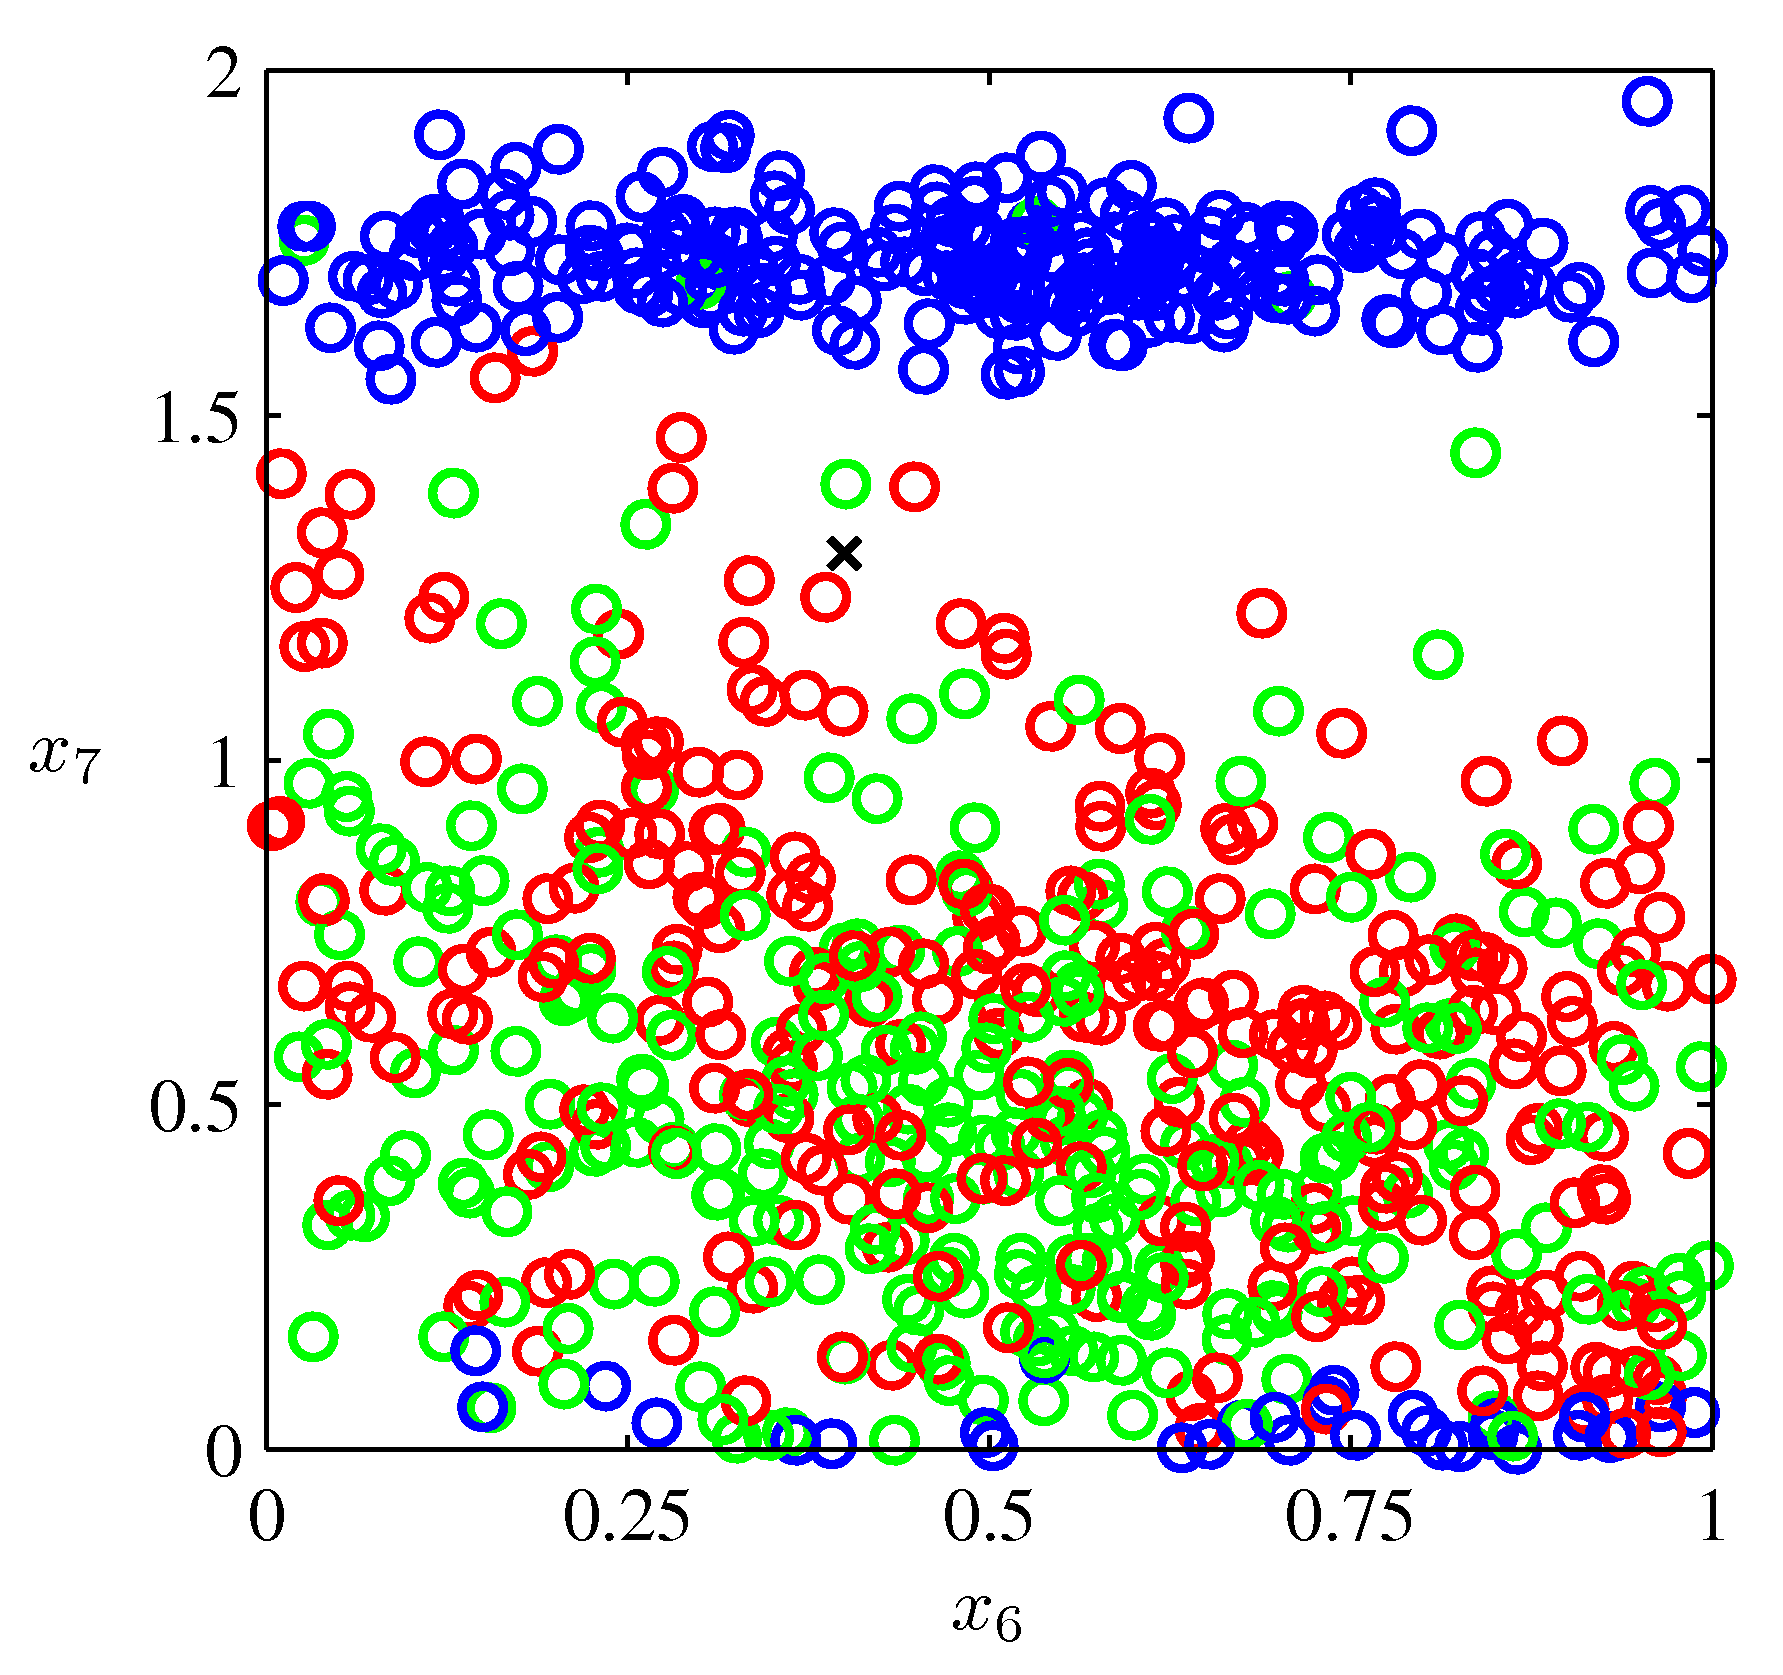
\includegraphics[scale=0.8]{Images/1-19.png}
		\captionsetup{font={small}}
		\caption{来自油流数据的输入量$x_6$,$x_7$的散点图,其中红色表示“均质”类,绿色代表“环状物”类,蓝色代表“层状物”类,我们的目标是将新的数据点“$\times$”进行分类。}
		\label{fig:1-19}
		\centering
		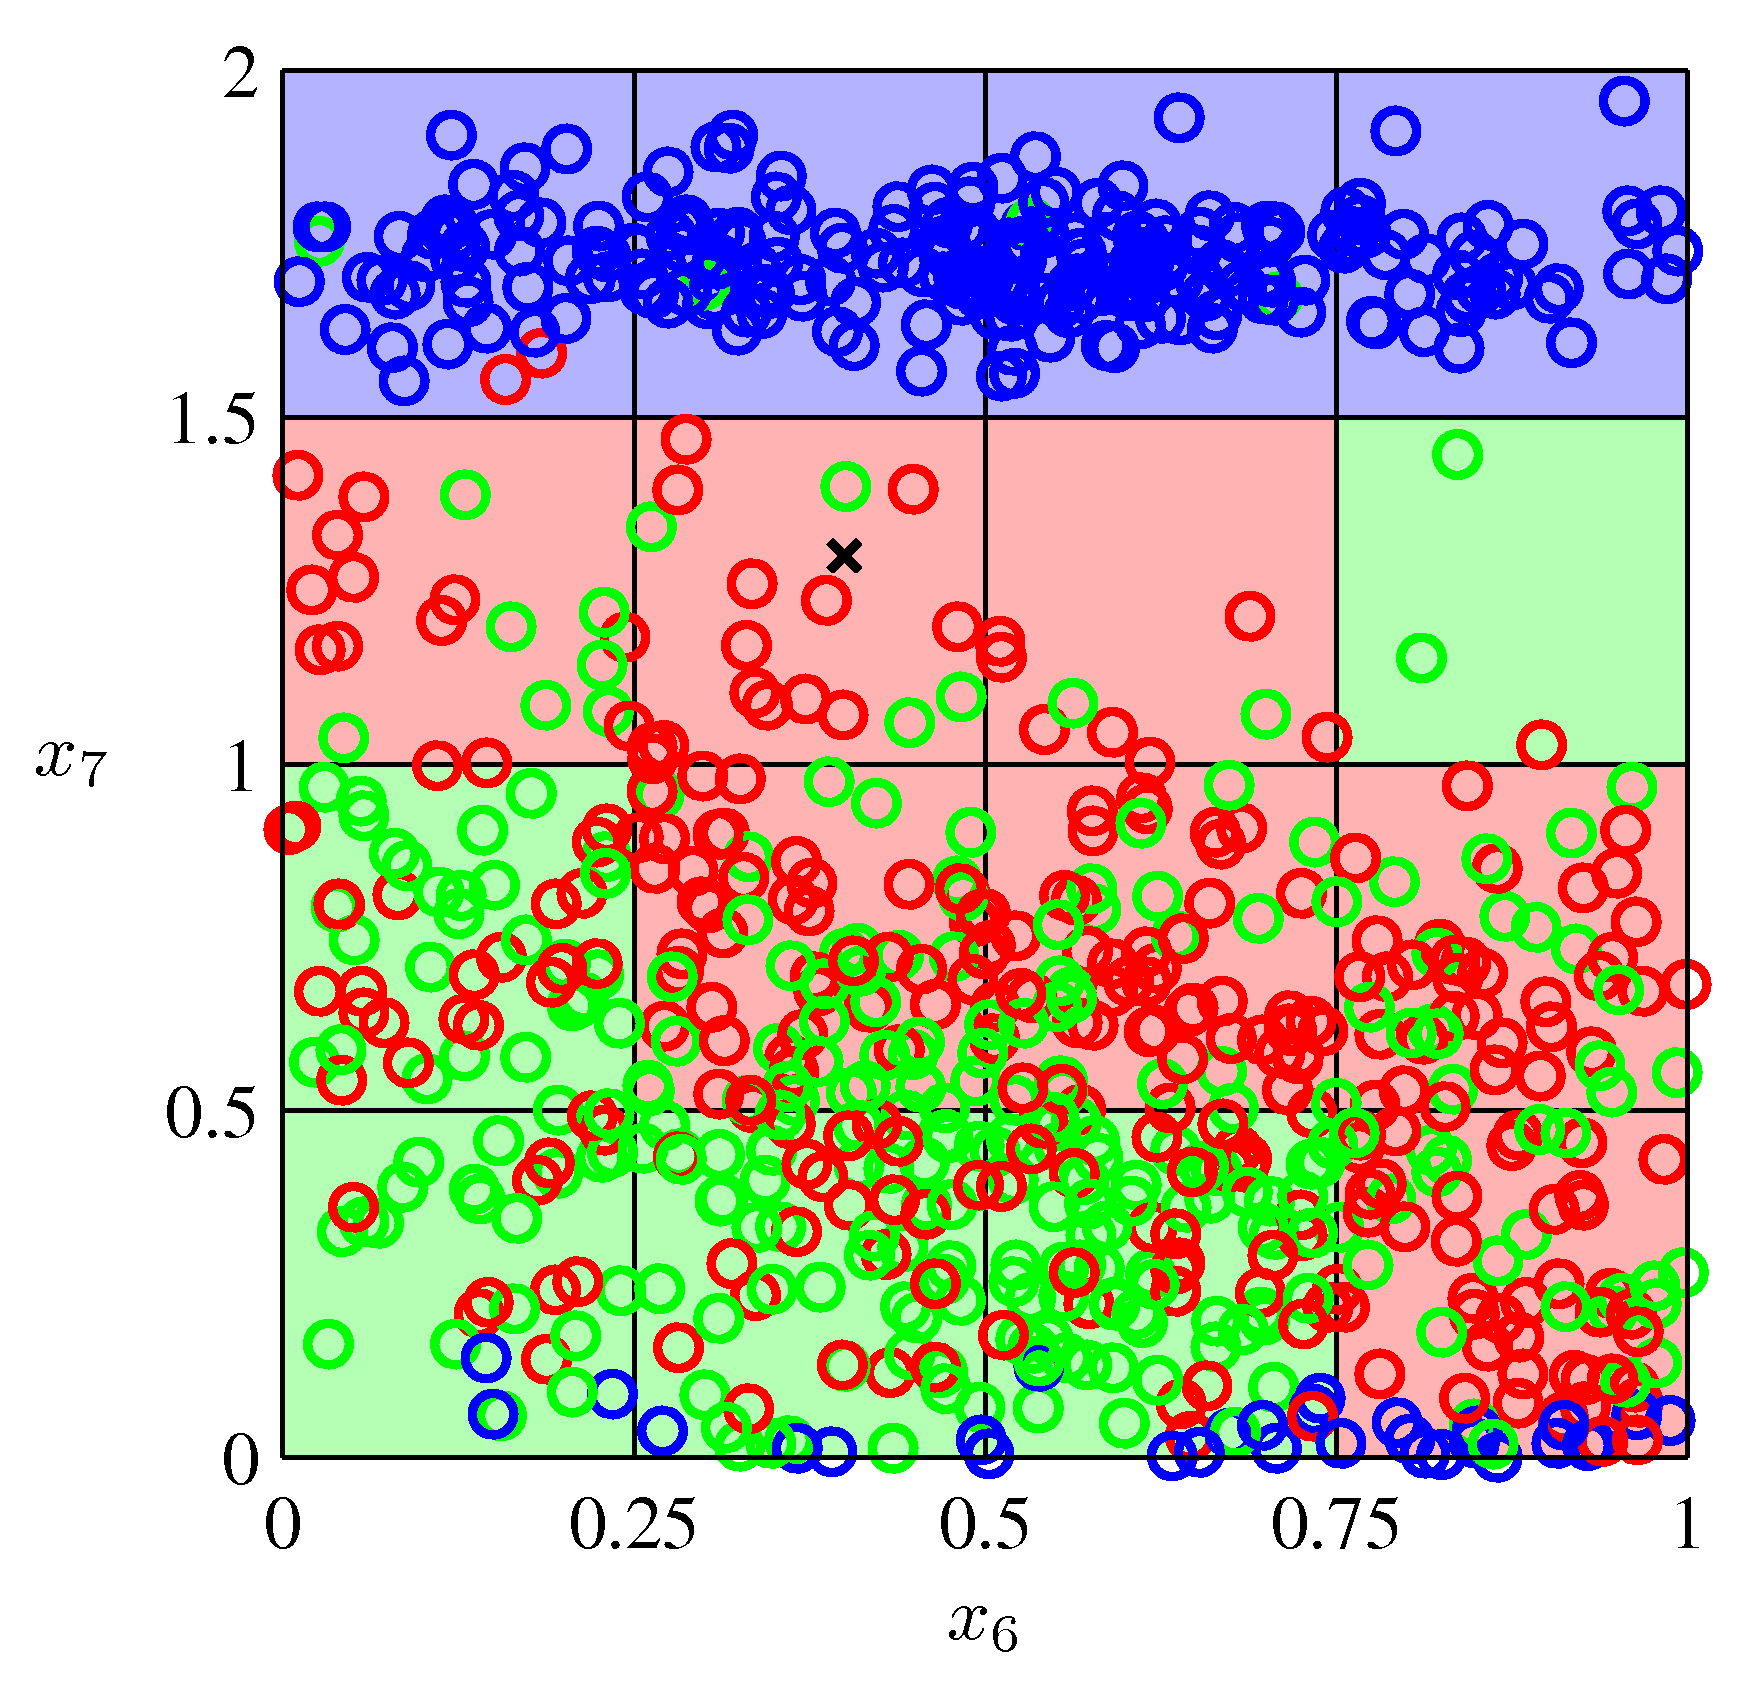
\includegraphics[scale=0.8]{Images/1-20.png}
		\captionsetup{font={small}}
		\caption{对于上述分类问题的一个简单方法,其中输入空间被划分成若干元组,对于任何的新测试点,其类别都会被预测为其所在元组中数量最多的那种数据点的类别。很快我们就会看到这样的办法有很多致命的缺点。}
		\label{fig:1-20}
	\end{figure}
	\\
	\indent 这个朴素的方法有成吨的问题。其中最要命的问题就是,当问题的输入变量数量变大时,对应地会使输入空间的维度变高。如图1.21所示就是这个问题的原始形态。其中展示了如果将空间区域分割成规则的元组,那么元组的数量会随着空间维度的上升而呈指数型地上涨。这样带来的问题是我们需要一个超级大的训练集才能保证元组是非空的。很明显,这样的办法在输入空间维度稍微高一点的时候就完蛋了,需要找到更好的办法。
	\begin{figure}[ht]
	\centering
		\begin{minipage}[t]{0.3\linewidth}
		\centering
		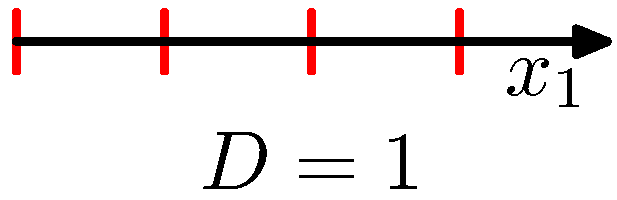
\includegraphics[scale=0.8]{Images/1-21a.png}
		\label{fig:1-21a}
		\end{minipage}
		\begin{minipage}[t]{0.3\linewidth}
		\centering
		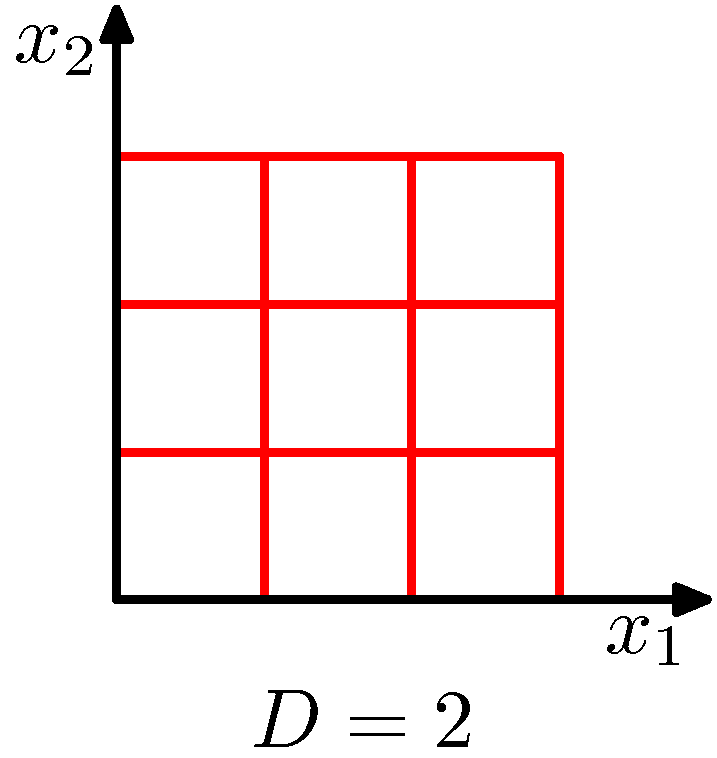
\includegraphics[scale=0.8]{Images/1-21b.png}
		\label{fig:1-21b}
		\end{minipage} 
		\centering
		\begin{minipage}[t]{0.3\linewidth}
		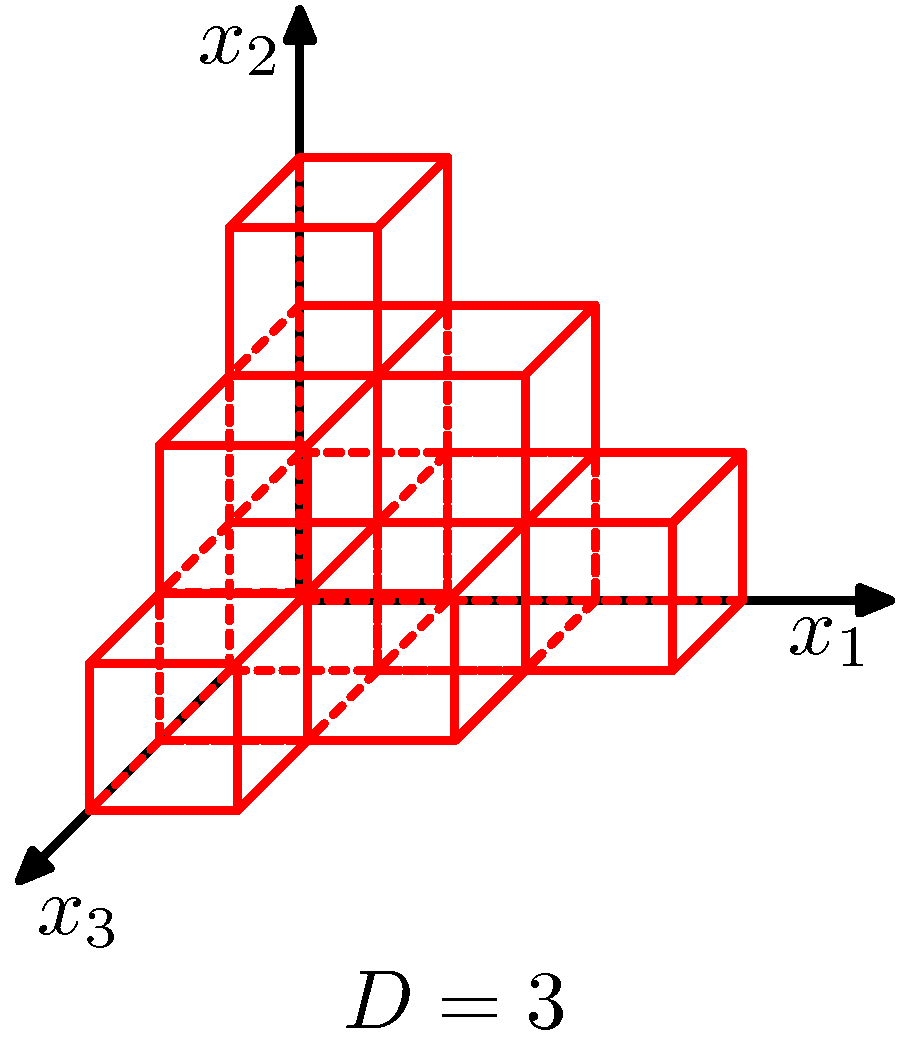
\includegraphics[scale=0.8]{Images/1-21c.png}
		\label{fig:1-21c}
		\end{minipage}
		\captionsetup{font={small}}
		\caption{维数灾难的示意图,展示了区域中格子的数量如何随着空间维度$D$的上升而呈指数型上涨。为了简洁,这里仅展示到$D=3$的情况。}
	\end{figure}
	\\
	\indent 对于高维空间的问题,我们可以通过回看多项式曲线拟合的案例来得到更加深刻的见解,同时研究一下如何将这项方法进行扩展,从而应对具有多个变量的输入空间。\color{red} \textbf{——第1.1节} \color{black}如果有$D$个输入变量,那么三阶多项式的通式为:
	\begin{equation}
		y(\boldsymbol{\mathrm{x}},\boldsymbol{\mathrm{w}})=w_0 + \sum_{i=1}^{D}{w_ix_i} + \sum_{i=1}^{D} \sum_{j=1}^{D}{w_{ij}x_ix_j} + \sum_{i=1}^{D}\sum_{j=1}^{D}\sum_{k=1}^{D}{w_{ijk}x_ix_jx_k}
	\end{equation}
	\indent 当$D$增加时,独立系数的数量(由于$x$变量之间的交换对称性,并非所有系数都是独立的)会按比例增加到$D^3$。在实践中,为了获取数据中复杂的依赖关系,可能会需要使用更高阶的多项式。对于一个阶数为$M$的多项式,系数的数量就会上升为$D^M$这样的了。\color{red} \textbf{——习题 1.16} \color{black}尽管现在是一个幂次上涨而非指数上涨,但躲得了初一躲不了十五,这个办法也会很快变得笨拙,在实用方面受到限制。\\
	\indent 在三维空间的显现实生活中形成的几何直觉会在我们研究高维空间时遭遇严重的打击。一个简单的例子是,对于一个$D$维空间中半径$r=1$的球体,求球体中位于$r=1-\epsilon$与$r=1$之间的体积。我们注意到$D$维空间中半径为$r$的球体体积单位一定是$r^D$,所以可以这样写:
	\begin{equation}
		V_D(r)=K_Dr^D
	\end{equation}
	其中系数$K_D$仅与$D$有关。于是所要求的体积可以写成:\color{red} \textbf{——习题 1.18} \color{black}
	\begin{equation}
		\frac{V_D(1)-V_D(1-\epsilon)}{V_D(1)}=1-(1-\epsilon)^D
	\end{equation}
	它可以被认为是在$D$取得不同数值时的$\epsilon$的函数,如图1.22所示。可以看出,对于较大的$D$,所求体积即使在$\epsilon$很小的情况下都是接近1的。于是,在高维的空间中,一个球体的大部分体积都集中在靠近表面的薄壳中!
	\begin{figure}[ht]
		\centering
		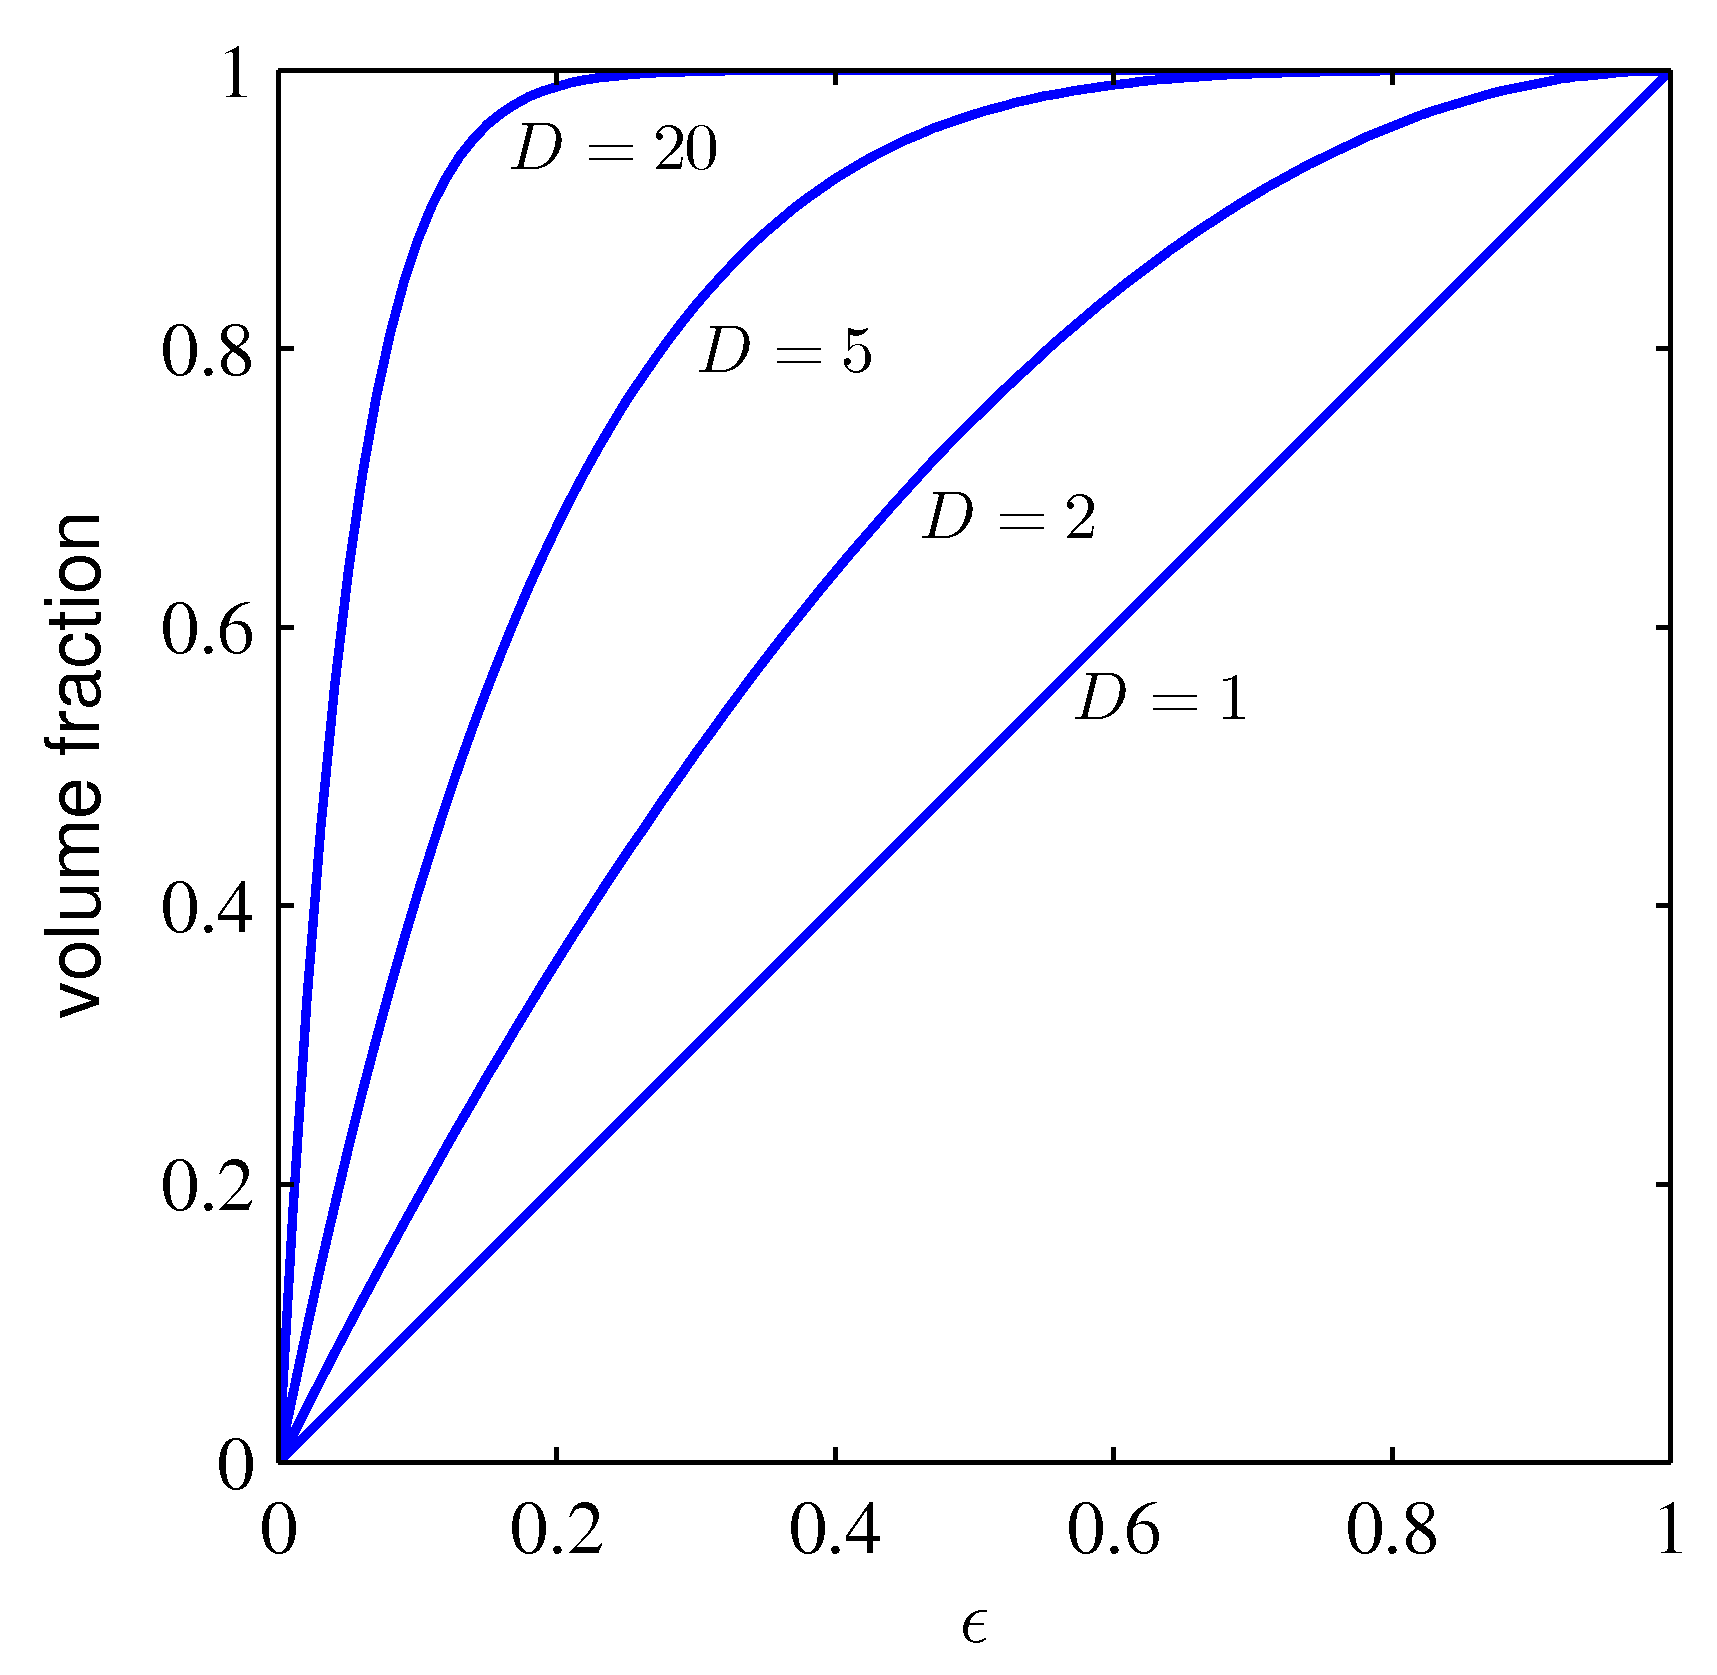
\includegraphics[scale=0.8]{Images/1-22.png}
		\captionsetup{font={small}}
		\caption{对于不同的$D$,球体中位于$r=1-\epsilon$与$r=1$之间的体积}
		\label{fig:1-22}
	\end{figure}
	\\
	\indent 作为与模式识别直接相关的另一示例,接下来研究一下高维空间中的高斯分布的特性。如果将笛卡尔坐标系变换为极坐标系,并对方向变量积分,就可以确定密度$p(r)$的表达式,$p(r)$是一个关于半径$r$的函数。所以$p(r)\delta r$就是位于$r$处厚度为$\delta r$的薄壳的概率质量。对于不同的$D$,分布的曲线如图1.23所示。我们可以看出对于较大的$D$,高斯分布的概率质量会集中在一个薄壳里。\color{red} \textbf{——习题 1.20} \color{black}
	\begin{figure}[ht]
		\centering
		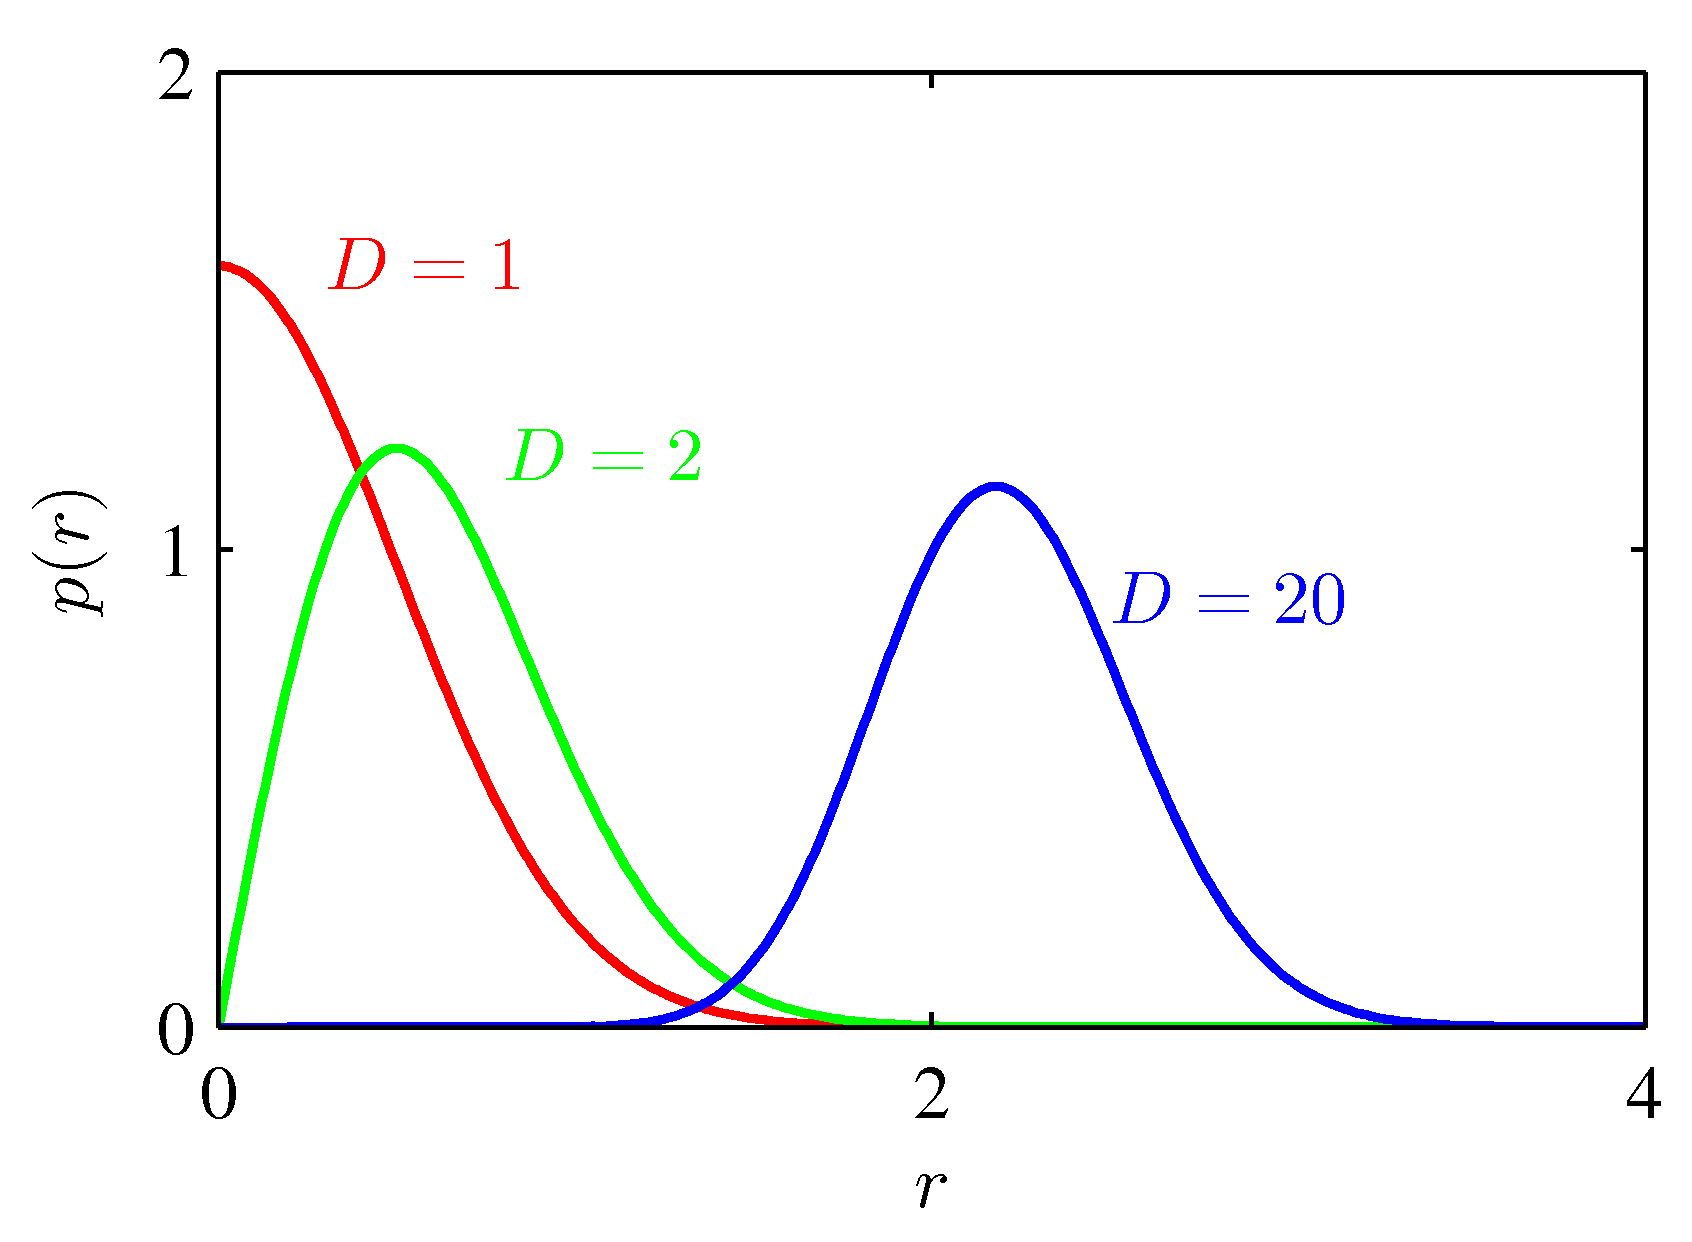
\includegraphics[scale=0.8]{Images/1-23.png}
		\captionsetup{font={small}}
		\caption{在维数$D$取不同值时关于$r$的高斯分布的概率密度。在高维的空间中,一个高斯分布的概率质量主要集中在特定半径位置的薄壳内。}
		\label{fig:1-23}
	\end{figure}
	\\
	\indent 这些可能在高维空间中出现的严重问题有时被称为维数灾难(curse of dimensionality, Bellman, 1961)。在本书中,我们会广泛使用输入空间为一维或二维空间中的例子,因为这样可以让各种图形表达更加清楚和简单。但读者应该留意,并非所有在低维空间中形成的习惯性直觉都可以推广到高维空间。\\
	\indent 尽管维数灾难确实是模式识别中的一个大麻烦,但这并不能阻止我们有效处理高维空间的问题。理由有两方面。首先,真实的数据往往都会被限制在较低有效维度的空间区域中,特别是在目标变量可能会发生重要变化的方向上。其次,真实的数据通常会表现出一些平滑性(至少在局部上),所以在大多数情况下,输入变量的微小变化也不会对目标变量产生太大的影响,因此可以使用类似于局部插值的方法对新的输入变量进行相应目标变量的预测。成功的模式识别技术一定会利用这些特性,要么利用其一,要么二者兼有。举例而言,让我们设想一种在生产制造中模式识别的应用,假设我们获取了某条传送带上某种特定平面物体的图像,要利用图像判断它们的方向。每张图像其实都是高维空间中的一个点,而这个高维空间的维度是由图像的像素数确定的。由于物体可能在图像中的任何位置出现,其方向也是随机的,所以图像之间存在3个可变自由度,而且这些图像会存在于高维空间中的一个三维流形(manifold)上。由于物体的位置和方向与像素强度之间的关系实在太复杂,这个流形会是高度非线性的。如果我们的目标改变为仅利用输入图像输出物体的方向,而不需要应对位置变化的问题,那么这个流形一下子就变成仅有1个可变自由度了。
	}
	\section{决策论}
	\noindent{\color{red} \rule[10pt]{\textwidth}{0.1em}}
	\textnormal{
	\indent 在1.2节中我们已经看到,概率论让我们可以利用这个连贯的数学框架来量化和控制不确定性。现在我们转向决策论的讨论,当决策论与概率论相结合,我们就可以有效应对含有不确定性的模式识别问题,并做出最优的决策。\\
	\indent 假设我们现在有一个输入向量$\boldsymbol{\mathrm{x}}$,它对应的目标向量是$\boldsymbol{\mathrm{t}}$,目标仍然是为新的$\boldsymbol{\mathrm{x}}$预测$\boldsymbol{\mathrm{t}}$。对于回归问题而言,$\boldsymbol{\mathrm{t}}$为连续变量,对于分类问题而言,$\boldsymbol{\mathrm{t}}$为类别标签。联合概率分布$p(\boldsymbol{\mathrm{x}},\boldsymbol{\mathrm{t}})$是对不确定性的完整概述,而不确定性是与变量密切相关的。利用训练数据集确定$p(\boldsymbol{\mathrm{x}},\boldsymbol{\mathrm{t}})$称为推断(inference),这个问题相当困难,以至于它的解决手段就构成了本书涉及到的很多学科。但是在实际应用中,对$\boldsymbol{\mathrm{t}}$做出具体的预测是不可避免的,而且更多的时候还要基于$\boldsymbol{\mathrm{t}}$的取值采取具体的行动,这就是决策论的研究内容。\\
	\indent 举例而言,假设我们现在有一个医学诊断问题,要通过病人的X光片来判断病人是否得了肿瘤。在这种情况下,输入向量$\boldsymbol{\mathrm{x}}$是来自图像的一系列像素强度,输出变量$t$表示肿瘤的存在与否,若肿瘤存在则分类为$\mathcal{C}_1$,反之为$\mathcal{C}_2$。我们可能会将$t$设定为二值变量,$t=0$对应类别$\mathcal{C}_1$,$t=1$对应类别$\mathcal{C}_2$。我们将在稍后看到这样取值对概率模型来说相当方便。这个推断问题接下来涉及到确定联合分布$p(\boldsymbol{\mathrm{x}},\mathcal{C}_k)$,或者其等价形式$p(\boldsymbol{\mathrm{x}},\boldsymbol{\mathrm{t}})$,从而给出这一问题的完整概率表述。尽管概率模型可以提供非常实用而且丰富的信息,但我们最终的目的还是确定这个患者是否需要治疗,而且我们当然希望做出的决策在某种意义上是最优的(Duda and Hart, 1973)。这就是决策(decision)步骤,而且决策论的主题就是告诉我们如何在给定了适当概率的情况下做出最优决策。我们将看到,一旦解决了推断问题,决策步骤就将是非常简单,甚至可以说是微不足道的。\\
	\indent 在这里我们会介绍一些本书后续内容要求掌握的决策论关键思想。对于更广泛的背景知识和更加详细的叙述,可以参考Berger(1985)和Bather(2000)的有关研究。\\
	\indent 在给出详细的分析之前,首先不太正式地研究一下概率论如何在决策中发挥重要的作用。当我们得到一个新病人的X光片$\boldsymbol{\mathrm{x}}$之后,我们要判定这张图像会指向两种结果中的哪一种。我们想要的是“给定图像的情况下结果分类的概率”,也就是$p(\mathcal{C}_k | \boldsymbol{\mathrm{x}})$。利用贝叶斯定理,这个概率可以表达为
	\begin{equation}
		p(\mathcal{C}_k | \boldsymbol{\mathrm{x}}) = \frac{p(\boldsymbol{\mathrm{x}}|\mathcal{C}_k)p(\mathcal{C}_k)}{p(\boldsymbol{\mathrm{x}})}
	\end{equation}
	需要注意的是,在贝叶斯定理中出现的任何值都可以利用联合分布$p(\boldsymbol{\mathrm{x}},\mathcal{C}_k)$对适当变量进行边缘化或条件化来得到。现在我们可以将$p(\mathcal{C}_k)$解释为类别$\mathcal{C}_k$的先验概率,将$p(\mathcal{C}_k | \boldsymbol{\mathrm{x}})$解释为对应的后验概率。因此,$p(\mathcal{C}_1)$表示在进行X光检测之前病人患有肿瘤的先验概率。类似地,$p(\mathcal{C}_1 | \boldsymbol{\mathrm{x}})$是其对应的后验概率,表示拿到X光检测结果之后利用其中的信息和贝叶斯定理对患有肿瘤的概率进行了修正。如果我们的目标是将$\boldsymbol{\mathrm{x}}$分类错误的可能性最小化,那么直觉上我们应当选择具有更高后验概率的那个类别。现在我们证明这个直觉是正确的,并讨论做决策的更加一般的标准。}
	\subsection{分类误差最小化}
	\textnormal{现在先假设我们的目标仅仅是要尽可能不出现分类错误的情况。为了给每个输入向量$\boldsymbol{\mathrm{x}}$分配一个合理的类别,我们肯定是需要依赖于一定的规则的。这样的规则会将整个输入空间分割成不同的区域$\mathcal{R}_k$,也就是决策域(decision regions),而且每个类别都对应一个决策域,于是$\mathcal{R}_k$中所有的点就都被分配了类别$\mathcal{C}_k$。决策域之间的边界被称为决策界(decision boundaries)或者决策面(decision surfaces)。需要注意的是,决策域并不一定是连在一起的,不相邻的区域也可以属于同一个决策域。我们会在后面的章节中讨论决策域和决策界的例子。在这里首先考虑二分类中寻找最优决策规则的问题,比如之前提及到的那个肿瘤诊断的例子,如果将一个实际上属于类别$\mathcal{C}_1$的输入分到了$\mathcal{C}_2$,那肯定是大错特错了,反过来也是一样。这种情况出现的概率可以表示为
	\begin{equation}
		\begin{split}
			p(\mathrm{mistake})&=p(\boldsymbol{\mathrm{x}}\in \mathcal{R}_1,\mathcal{C}_2) + p(\boldsymbol{\mathrm{x}}\in \mathcal{R}_2,\mathcal{C}_1) \\
			&=\int_{\mathcal{R}_1}p(\boldsymbol{\mathrm{x}},\mathcal{C}_2) \ \mathrm{d}\boldsymbol{\mathrm{x}} + \int_{\mathcal{R}_2}p(\boldsymbol{\mathrm{x}},\mathcal{C}_1) \ \mathrm{d}\boldsymbol{\mathrm{x}}
		\end{split}
	\end{equation}
	\indent 根据决策规则可以给每个$\boldsymbol{\mathrm{x}}$分配两种类别中的一个,而且这个决策规则是我们自行选择的。很明显,为了让$p(\mathrm{mistake})$尽可能地小,那么将$\boldsymbol{\mathrm{x}}$分配到哪种类别能让(1.78)中的积分式最小,就应该将其分到哪种类别。所以,如果$p(\boldsymbol{\mathrm{x}},\mathcal{C}_1)>p(\boldsymbol{\mathrm{x}},\mathcal{C}_2)$,那就应该把$\boldsymbol{\mathrm{x}}$归类到$\mathcal{C}_1$。根据概率论的乘法规则,我们有$p(\boldsymbol{\mathrm{x}},\mathcal{C}_k)=p(\mathcal{C}_k|\boldsymbol{\mathrm{x}})p(\boldsymbol{\mathrm{x}})$。由于两个积分项中的$p(\boldsymbol{\mathrm{x}})$是一样的,所以实际上那个初始的问题就可以转化为,对每个$\boldsymbol{\mathrm{x}}$分配一个使得后验概率$p(\mathcal{C}_k|\boldsymbol{\mathrm{x}})$最大的类别。图1.24所示的就是对于一个一元输入变量$x$进行二分类的问题。
	\begin{figure}[ht]
		\centering
		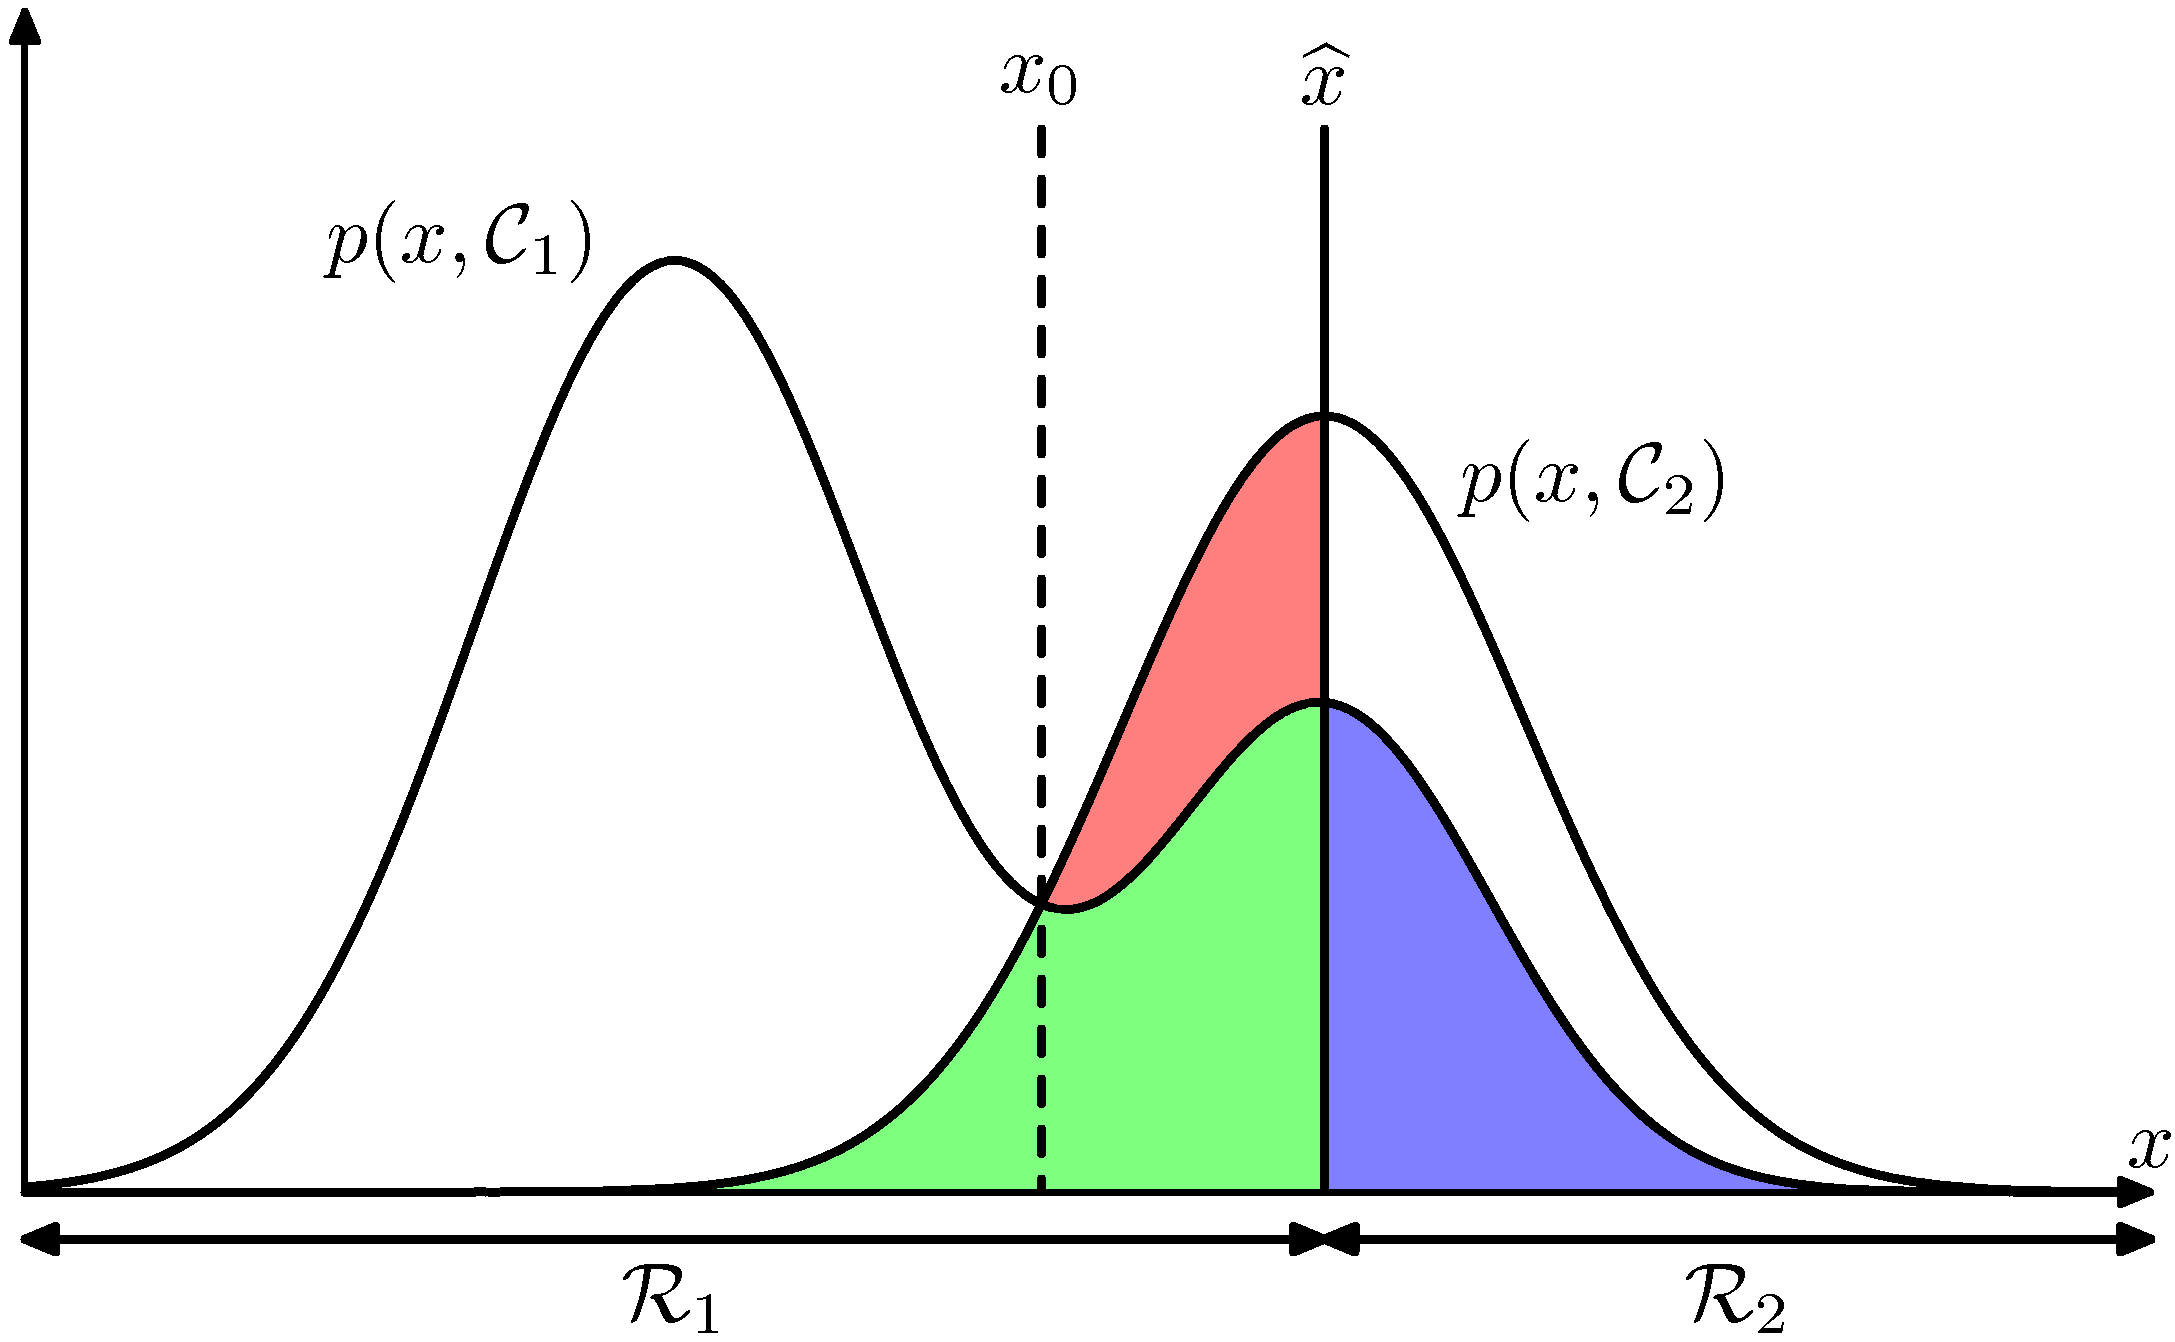
\includegraphics[scale=0.8]{Images/1-24.png}
		\captionsetup{font={small}}
		\caption{在二分类问题中两种类别分别关于$x$的联合概率$p(x,\mathcal{C}_k)$,同时指出了决策界$x=\hat{x}$的示意图。若$x \geqslant \hat{x}$则分类为$\mathcal{C}_2$,所以是属于决策域$\mathcal{R}_2$的,反过来,如果$x < \hat{x}$则分类为$\mathcal{C}_1$,属于决策域$\mathcal{R}_1$。分类错误来源于蓝色、绿色和红色区域,在$x < \hat{x}$的情况中,产生的错误主要是将本属于$\mathcal{C}_2$的$x$分类成$\mathcal{C}_1$,也就是红色区域和绿色区域的总和;反过来,在$x \geqslant \hat{x}$的情况中,产生的错误主要是将本属于$\mathcal{C}_1$的$x$分类成$\mathcal{C}_2$,也就是蓝色区域了。当我们改变决策域$\hat{x}$的位置,由于绿色区域和蓝色区域连在一起,它们的总和是不变的,而红色区域的大小是会发生变化的。决策域$\hat{x}$的最佳选择,应该是两条曲线$p(x,\mathcal{C}_1)$和$p(x,\mathcal{C}_2)$的相交处,也就是图中$x_0$的位置,因为在这里,红色区域就完全消失了。对于分类误差最小化问题的决策规则也是这样,实质上就是要将$x$归类于后验概率$p(\mathcal{C}_k|x)$更高的那一类。}
		\label{fig:1-24}
	\end{figure}
	\\
	\indent 对于更加一般的$K$分类问题,写成正确概率最大化的形式会更简单一些,也就是
	\begin{equation}
		\begin{split}
			p(\mathrm{correct})&=\sum_{k=1}^{K}p(\boldsymbol{\mathrm{x}}\in \mathcal{R}_k,\mathcal{C}_k)\\
			&=\sum_{k=1}^{K}\int_{\mathcal{R}_k}p(\boldsymbol{\mathrm{x}},\mathcal{C}_k)\ \mathrm{d}\boldsymbol{\mathrm{x}}
		\end{split}	
	\end{equation}
	这项概率会在$\boldsymbol{\mathrm{x}}$分配到使得$p(\boldsymbol{\mathrm{x}},\mathcal{C}_k)$取得最大值的决策域时达到最大值。再次利用乘法规则$p(\boldsymbol{\mathrm{x}},\mathcal{C}_k)=p(\mathcal{C}_k|\boldsymbol{\mathrm{x}})p(\boldsymbol{\mathrm{x}})$,并且再次留意到对于每个积分项来说$p(\boldsymbol{\mathrm{x}})$都是相同的,我们发现$\boldsymbol{\mathrm{x}}$应该分类到具有最大后验概率$p(\mathcal{C}_k|\boldsymbol{\mathrm{x}})$的类别。
	}
	\subsection{期望损失最小化}
	\textnormal{在很多的应用中,我们的目标不仅仅是将分类误差进行最小化,而往往是要更复杂一些。还是回到之前那个肿瘤诊断的问题,我们注意到,如果一个没有肿瘤的病人被误诊为患有肿瘤,那么会给病人带来无端的痛苦和后续的进一步诊断。而反过来,如果一个患有肿瘤的病人被认为是没有患病,那可能会导致病人没有得到及时的治疗最后翘辫子。很明显,比起第一种,第二种错误造成的后果要更加严重,所以宁可让第一种错误多犯一些,也要削减第二种错误出现的可能性。\\
	\indent 我们可以将这个问题写成损失函数(loss function)或者叫做代价函数(cost function)的形式。损失函数,是衡量在决策中采取任何一种决策或行动而造成的损失的单值标准。我们的目标是尽可能地减少总体损失。不过在其他的研究中,一些研究人员将这个问题视为效益函数(utility function)最大化的问题,其实和损失函数最小化是等价的,只需将损失取相反数就可以了,现在我们采用的是损失函数的形式。对于一个新的$\boldsymbol{\mathrm{x}}$,假设其真实类别是$\mathcal{C}_k$,而我们将其分类为$\mathcal{C}_j$——$j$可能等于$k$,也可能不等于$k$。这样做的结果,就是造成了损失$L_{kj}$,这个损失可以被看成是损失矩阵(loss matrix)中的$(k,j)$元素。举例而言,在肿瘤诊断的例子中,我们可以将损失矩阵设置成如图1.25所示的形式。这个损失矩阵表示的是,在分类正确的时候不会造成任何损失,如果将健康病人误诊为患有肿瘤,那么损失是1,而如果将一个患有肿瘤的病人误诊为健康,那么损失就是1000。
	\begin{figure}[ht]
		\centering
		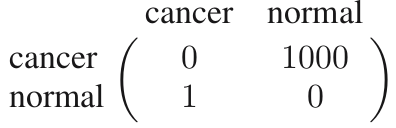
\includegraphics[scale=0.25]{Images/1-25.png}
		\captionsetup{font={small}}
		\caption{肿瘤诊断问题中的损失矩阵示例。每一行表示真实类别,每一列表示根据决策规则得出的分类结果。}
		\label{fig:1-25}
	\end{figure}
	\\
	\indent 最佳的解决方案,就是让损失函数最小的那一种。然而,损失函数是与真实类别有关的,而真实类别往往却是未知的。对于给定的输入变量$\boldsymbol{\mathrm{x}}$,其真实类别的不确定性是通过联合概率分布$p(\boldsymbol{\mathrm{x}},\mathcal{C}_k)$来表示的,所以我们需要一个替代方案,求取平均损失,而这个平均损失是根据联合概率分布求得的,可以表示为
	\begin{equation}
		\mathbb{E}[L]=\sum_k \sum_j \int_{\mathcal{R}_j}L_{kj}p(\boldsymbol{\mathrm{x}},\mathcal{C}_k)\ \mathrm{d}\boldsymbol{\mathrm{x}}
	\end{equation}
	任意的$\boldsymbol{\mathrm{x}}$都可以被指派到决策域之一$\mathcal{R}_j$中。我们的任务就是选择合适的$\mathcal{R}_j$,从而使得(1.80)中的期望损失最小,也就是说对于任意的$\boldsymbol{\mathrm{x}}$我们需要将$\sum_k L_{kj}p(\boldsymbol{\mathrm{x}},\mathcal{C}_k)$进行最小化。和往常一样,这里也可以用乘法规则$p(\boldsymbol{\mathrm{x}},\mathcal{C}_k)=p(\mathcal{C}_k|\boldsymbol{\mathrm{x}})p(\boldsymbol{\mathrm{x}})$,然后省略掉共同的因子$p(\boldsymbol{\mathrm{x}})$。所以使得期望损失最小的决策规则就是,给每个新的$\boldsymbol{\mathrm{x}}$分配的类别$j$应当使
	\begin{equation}
		\sum_k L_{kj}p(\mathcal{C}_k|\boldsymbol{\mathrm{x}})
	\end{equation}
	最小化。一旦我们知道了后验分类概率$p(\mathcal{C}_k|\boldsymbol{\mathrm{x}})$,这个问题就是轻而易举的了。
	}
	\subsection{拒绝选项}
	\textnormal{我们已经看到分类误差源自于输入空间中这样的一些区域中——区域中最大的后验概率$p(\mathcal{C}_k|\boldsymbol{\mathrm{x}})$明显低于整体水平,或者等价地说,区域中各个联合分布$p(\boldsymbol{\mathrm{x}},\mathcal{C}_k)$的值比较势均力敌。在这些区域里,该怎样进行分类是比较让人头疼的一件事。在实际应用中,为了让错误率低一些,比较明智的做法是直接逃避,避免在这些容易导致分类错误的样例上做决策,所谓“君子不立于危墙之下”,这就是拒绝选项(reject option)。比如说,在肿瘤诊断的问题中,可以利用一个自动分类系统,将诊断结果可能存在疑问的那些X光片挑选出来,再由专家进行人工的判断,从而得到更加准确的结果。我们可以通过设定一个阈值$\theta$来实现这项功能,将最大后验概率$p(\mathcal{C}_k|\boldsymbol{\mathrm{x}})$低于或等于$\theta$的输入$\boldsymbol{\mathrm{x}}$全部拒绝掉。图1.26所示是对于一个一元输入变量$x$进行二分类的示例。需要注意的是,将阈值设置为$\theta =1$就是将全部输入样例都拒绝掉,同时,对于$K$分类问题,将阈值设置为$\theta < 1/K$就是不拒绝任何输入样例了。所以输入样例中被拒绝的比例取决于$\theta$的值。
	\begin{figure}[ht]
		\centering
		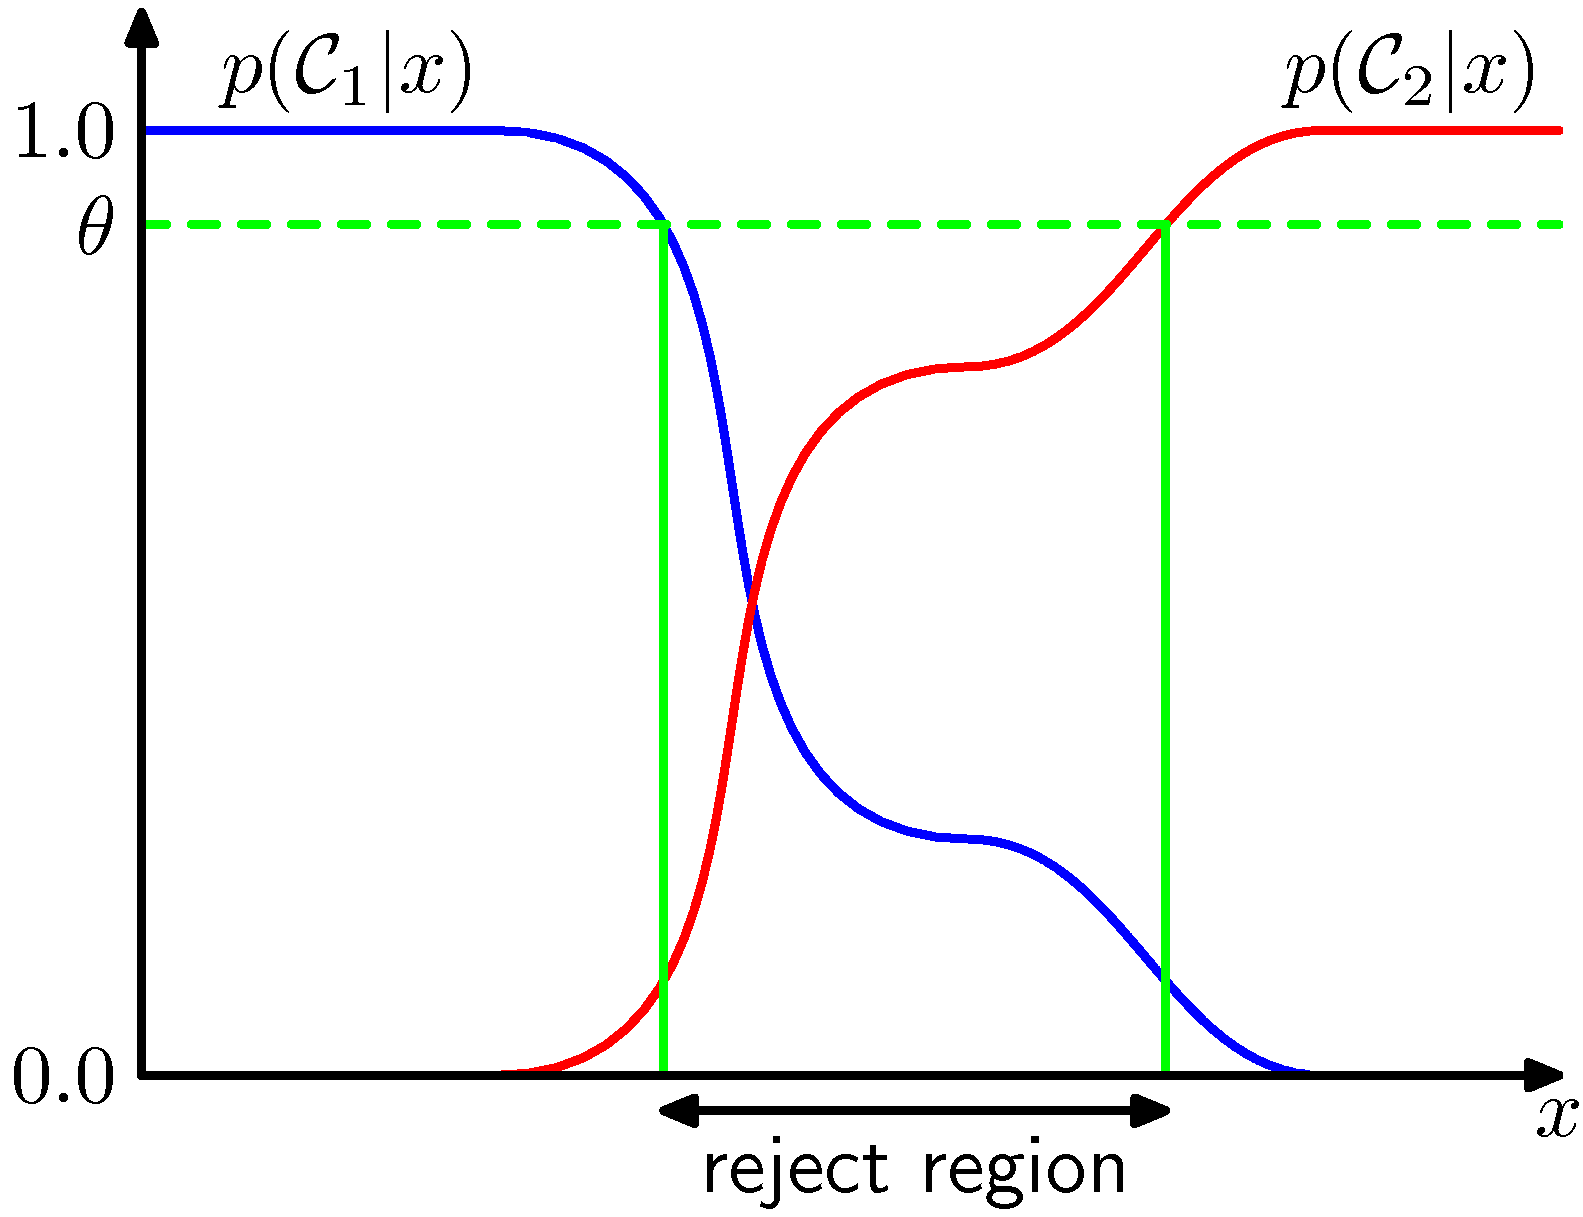
\includegraphics[scale=0.8]{Images/1-26.png}
		\captionsetup{font={small}}
		\caption{拒绝选项示意图。当两个后验概率中的最大值小于或等于某个阈值$\theta$时,这个输入$x$就会被拒绝。}
		\label{fig:1-26}
	\end{figure}
	\\
	\indent 当损失矩阵已知的情况下,我们可以很轻松地将拒绝选项引到期望误差最小化中,从而考虑做出拒绝的决定时造成的损失。\color{red} \textbf{——习题 1.24} \color{black}}
	\subsection{推断与决策}
	\textnormal{我们已经将分类问题拆分成两个步骤,在推断步骤(inference stage),我们利用训练数据来学习一个$p(\mathcal{C}_k|\boldsymbol{\mathrm{x}})$的模型,而在后续的决策步骤(decision stage),我们会利用这些后验概率来进行最优的分类。一个二选一的概率可以将这两个问题一同解决,只需要学习一个直接将输入$\boldsymbol{\mathrm{x}}$指向决策结果的函数就可以了。这样的函数被称为判别函数(discriminant function)。\\
	\indent 实际上,解决决策问题有三种不同的方法,它们都可以用于实际应用中,而且我们可以明确地辨认它们。根据复杂程度降序排列,这些方法分别是:\\
	\textbf{(a)}\ 首先解决推断问题,也就是确定分类——对于每一种类别$\mathcal{C}_k$求取条件概率密度$p(\boldsymbol{\mathrm{x}}|\mathcal{C}_k)$。同时还要分别确定分类先验概率$p(\mathcal{C}_k)$。然后采用如下形式的贝叶斯定理
	\begin{equation}
		p(\mathcal{C}_k|\boldsymbol{\mathrm{x}})=\frac{p(\boldsymbol{\mathrm{x}}|\mathcal{C}_k)p(\mathcal{C}_k)}{p(\boldsymbol{\mathrm{x}})}
	\end{equation}
	来求取分类后验概率$p(\mathcal{C}_k|\boldsymbol{\mathrm{x}})$。和往常一样,贝叶斯定理中的分母可以写成分子求和的形式,因为
	\begin{equation}
		p(\boldsymbol{\mathrm{x}})=\sum_k p(\boldsymbol{\mathrm{x}}|\mathcal{C}_k)p(\mathcal{C}_k)
	\end{equation}
	等价地,我们也可以直接建立联合分布$p(\boldsymbol{\mathrm{x}},\mathcal{C}_k)$,然后进行归一化,以得到后验概率。得到后验概率之后,利用决策论来确定每个新的输入$\boldsymbol{\mathrm{x}}$的分类。或明确或隐含地对输入和输出进行建模的方法被称为生成模型(generative models),因为通过在其中采样就可以在输入空间生成数据点。\\
	\textbf{(b)}\ 首先解决推断问题,但先确定后验分类概率$p(\mathcal{C}_k|\boldsymbol{\mathrm{x}})$,然后利用决策论,为每个新的$\boldsymbol{\mathrm{x}}$进行分类。这种直接利用后验概率的方法称为判别模型(discriminative models)。\\
	\textbf{(c)}\ 寻找将输入$\boldsymbol{\mathrm{x}}$直接映射到分类标签的判别函数$f(\boldsymbol{\mathrm{x}})$。举例而言,在二分类问题中,$f(\cdot)$应该是一个二值函数,$f=0$表示类别$\mathcal{C}_1$,$f=1$表示类别$\mathcal{C}_2$。在这种情况中,概率论没有发挥作用。\\
	\indent 接下来研究这三种方法各自的优点。方法(a)是要求最多的,因为要找到$\boldsymbol{\mathrm{x}}$和$\mathcal{C}_k$的联合分布。在很多实际应用中,$\boldsymbol{\mathrm{x}}$的维度可能是很高的,所以我们可能需要很大的训练集来保证分类的条件概率密度函数是充分准确的。需要注意的是,分类先验$p(\mathcal{C}_k)$通常可以比较简单地利用训练数据中属于各个分类的样本比例进行估计。但方法(a)的一大优点,就是可以利用(1.83)确定数据的边缘概率密度$p(\boldsymbol{\mathrm{x}})$。这对于在模型下概率较低的和预测准确率较低的新数据是相当有用的,这个过程称为离群点检测(outlier detection) 或称为异常检测(novelty detection)(Bishop, 1994;Tarassenko, 1995)。\\
	\indent 然而,如果我们仅仅希望做出分类决策,那方法(a)中求取$p(\boldsymbol{\mathrm{x}},\mathcal{C}_k)$就很浪费计算资源了,而且对数据数量的要求太高,毕竟夯不啷当算了一大堆,其实用得上的只不过是$p(\mathcal{C}_k|\boldsymbol{\mathrm{x}})$而已,这种时候用方法(b)就直接得多了。毕竟分类的条件概率密度可能包含了一大堆对于后验概率没什么作用的内容,如图1.27所示。顺便一提,人们一直在探索机器学习中生成模型方法和判别模型方法各自的优点,而且对将两种方法结合起来的办法一直很感兴趣(Jebara, 2004; Lasserre et al., 2006)。
	\begin{figure}[ht]
		\begin{minipage}[t]{0.5\linewidth}
		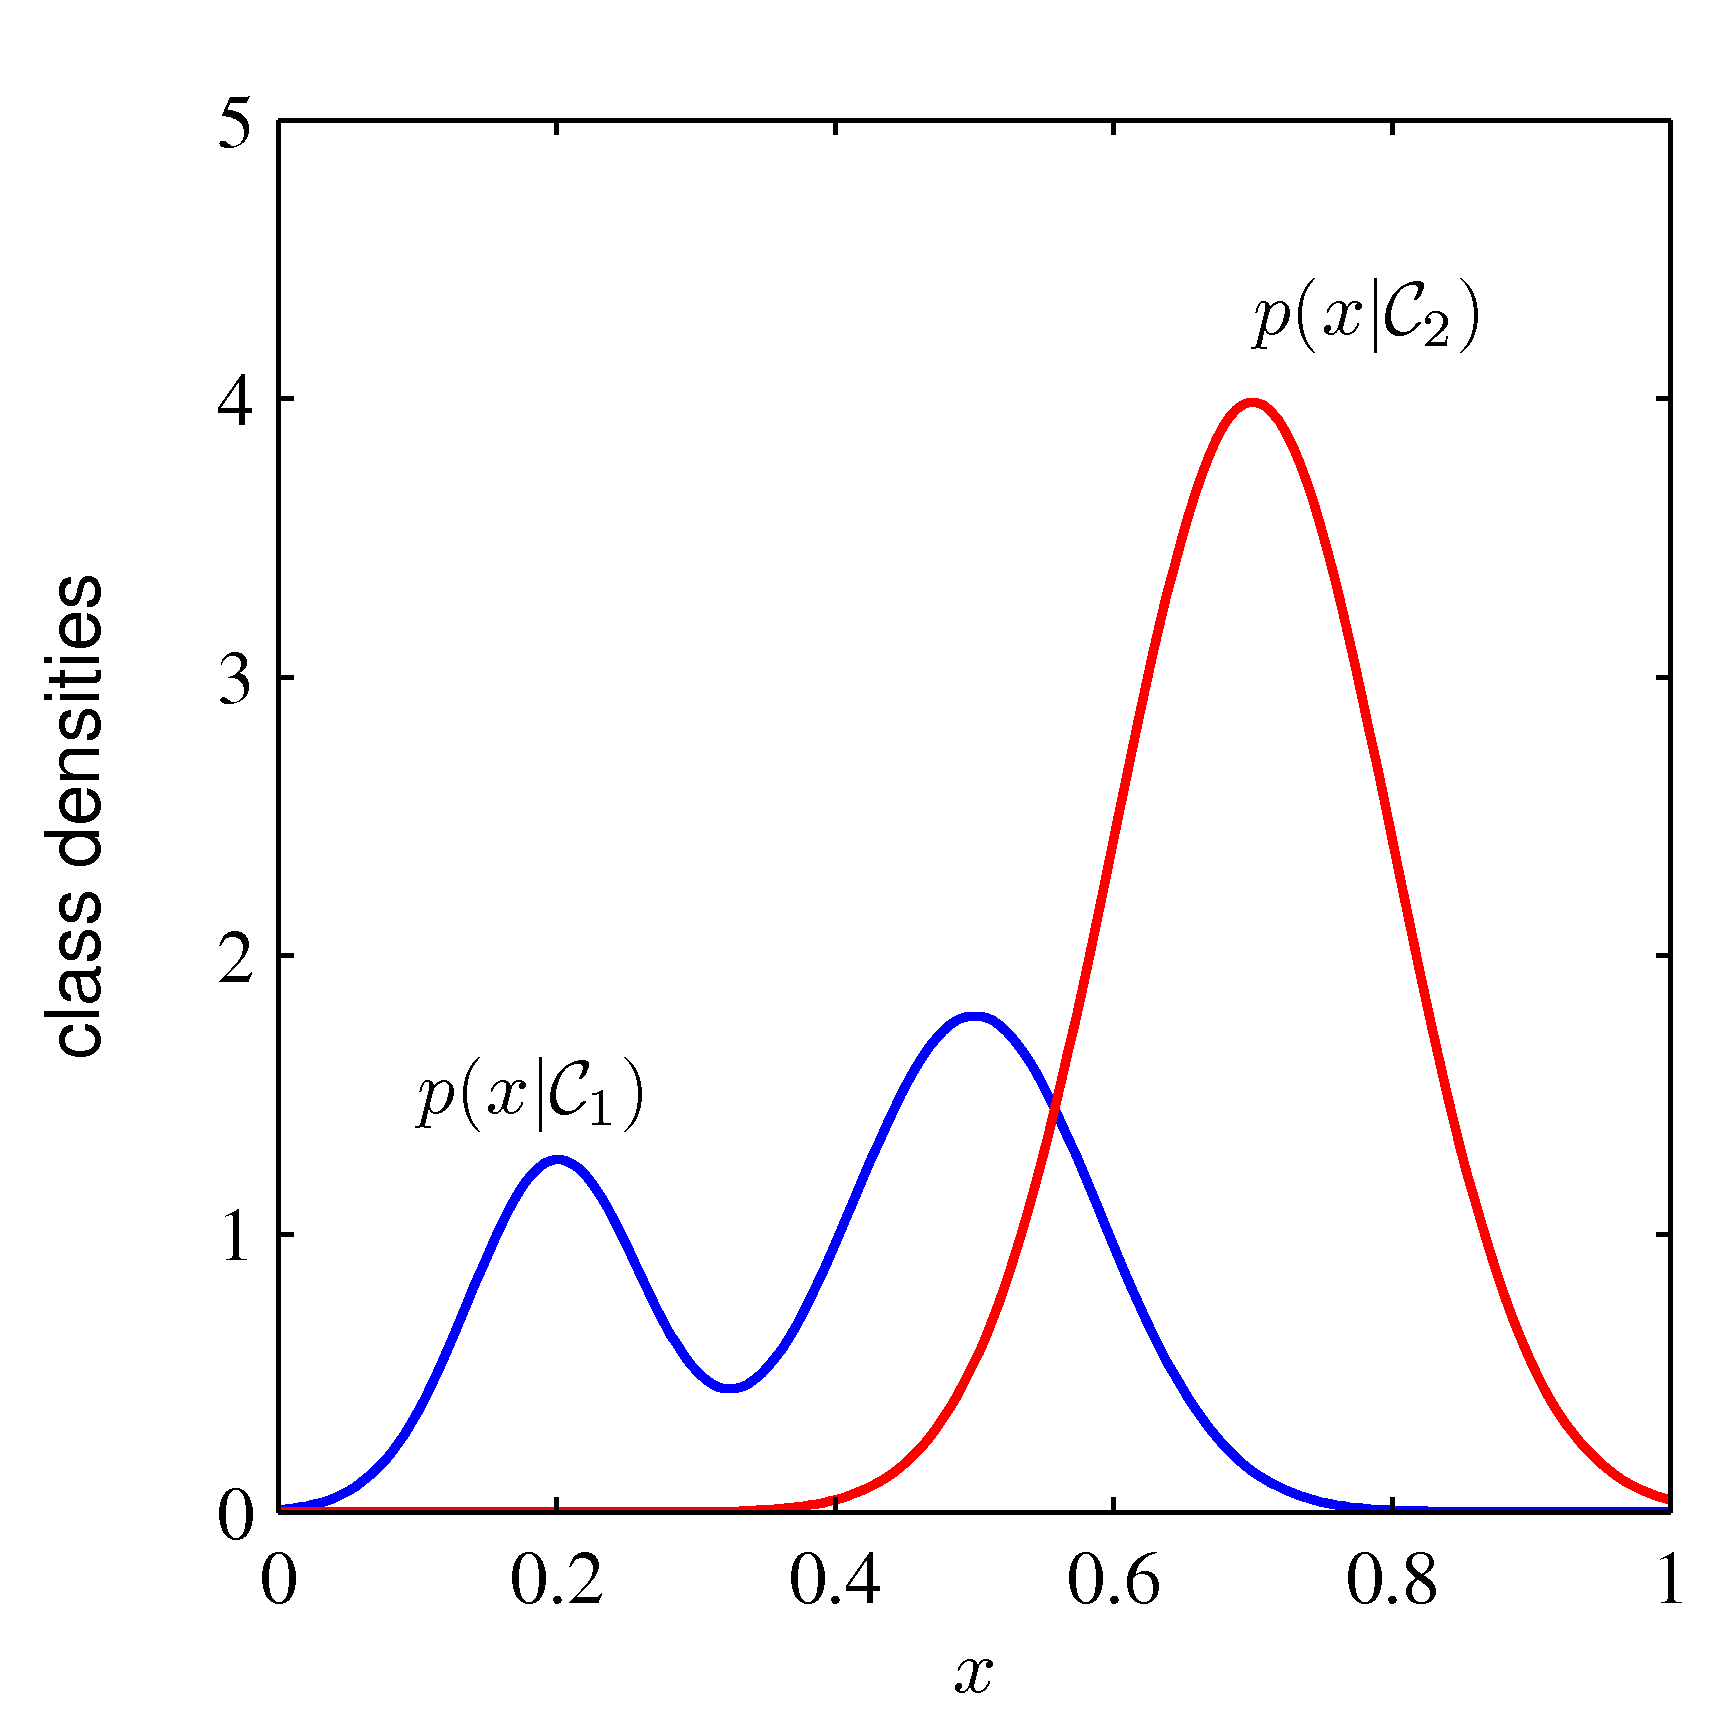
\includegraphics[scale=0.8]{Images/1-27a.png}
		\label{fig:1-27a}
		\end{minipage}
		\begin{minipage}[t]{0.5\linewidth}
		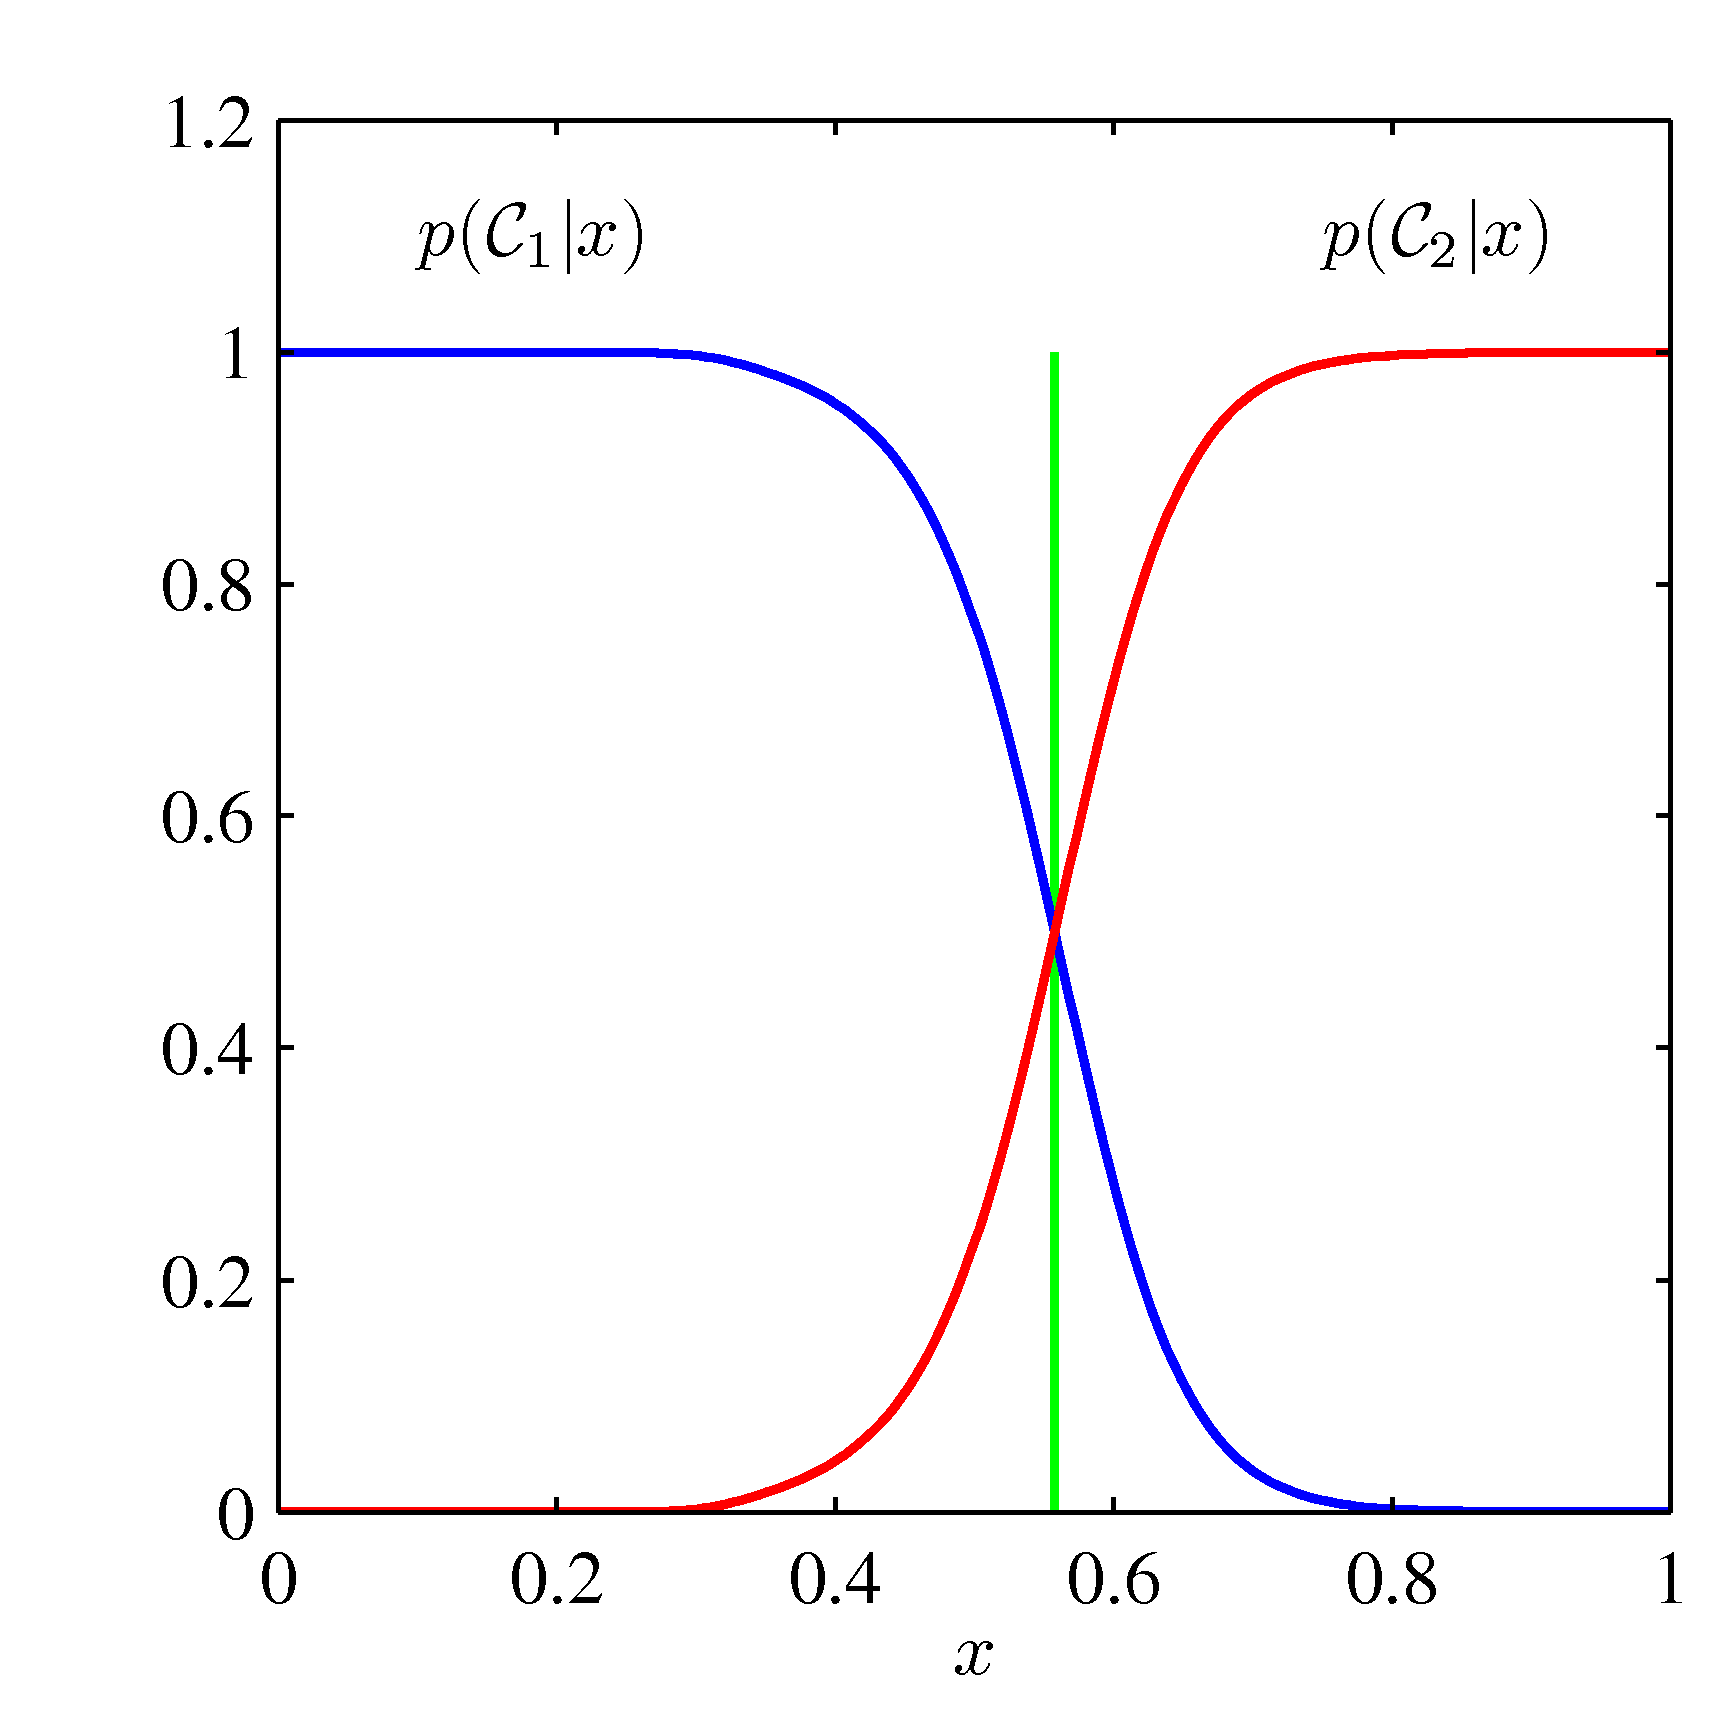
\includegraphics[scale=0.8]{Images/1-27b.png}
		\label{fig:1-27b}
		\end{minipage} 
		\captionsetup{font={small}}
		\caption{对一元输入变量$x$进行两种分类的条件概率密度(左图)和对应的后验概率(右图)。需要注意的是,左图中表示为蓝色曲线的分类条件概率密度$p(\boldsymbol{\mathrm{x}}|\mathcal{C}_k)$对于后验概率没有影响。右图中垂直的绿线表示的是假设分类的先验概率$p(\mathcal{C}_1)$和$p(\mathcal{C}_2)$相等的情况下,关于$x$的使得分类误差率最小的决策界。}
	\end{figure}
	\\
	\indent 方法(c)就更加简单了,只需要寻找分类函数$f(\boldsymbol{\mathrm{x}})$,将$\boldsymbol{\mathrm{x}}$映射到某种类别标签,于是就将推断和决策步骤结合成单一的学习问题了。如图1.27中的示例所示,这个方法是要找出垂直绿线对应的$x$值,因为这就是使得错误分类概率最小的决策界。\\
	\indent 但是,方法(c)会让我们无从获得后验概率$p(\mathcal{C}_k|\boldsymbol{\mathrm{x}})$。然而后验概率又是很必要的,即使是在后面做决策的时候都是很有用处的。理由包括:\\
	\indent \textbf{风险最小化。}让我们考虑这样的一个问题——损失矩阵里的元素会时刻发生变化,这种情况可能会出现在金融领域的应用中。如果我们知道后验概率,就可以轻而易举地通过修改(1.81)来修改决策标准,从而使风险最小化。如果我们只有判定函数,那么一旦损失矩阵发生任何变化,我们就必须重新进行训练,从头开始解决这个分类的问题。\\
	\indent \textbf{拒绝选项。}后验概率使得我们可以根据拒绝数据点的数量确定一个拒绝的标准,从而降低分类的错误率和减小期望损失。\\
	\indent \textbf{补偿分类先验。}还是拿X光诊断的问题说事。假设我们已经从公众群体中拿到了一个很大的X光片数据集来作为训练数据,从而构建一个自动诊断系统。由于在公众中肿瘤还是比较少见的,我们可能会发现1000例数据中才有1例是有肿瘤表现的。如果我们用这样的数据集去训练模型,由于患肿瘤的样本实在太少了,训练会遇到很多超级大麻烦。比如说,可能会得到一个将所有的输入数据都判定为属于未患病类别的分类器,而且还是有着99.9\% 准确率的那种,而且这种明显不对的结果还特别难以回避。另外,即使是很大的数据集也不会有多少样例是患有肿瘤的,所以学习算法的学习范围太狭窄了,不会有很好的泛化能力。只有那种各类样例数量差不多的,比较均衡的数据集才能够训练出准确的模型。然而如果这样做的话,就需要对训练数据的修正进行补偿。假设我们用这样经过修正的数据集得到了后验概率,根据贝叶斯定理(1.82),可以看出后验概率是与先验概率成比例的,而先验概率实际上就是每种类别的数据所占的比例。所以我们就可以利用从人工均衡过的数据集得到的后验概率,首先除以数据集中的类别比例,再乘以我们希望应用模型的公众中的类别比例。最后还需要对新得到的后验概率进行正则化,确保其总和为1。如果是直接学习了判别函数而不考虑后验概率的话,这个过程就不能进行了。\\
	\indent \textbf{联合模型。}对于复杂的应用来说,我们可能希望把问题拆分成很多小一点的子问题,每个子问题都当成是一个独立的单元来处理。比如之前那个诊断的问题,没准除了X光片我们还有其他的检测结果,比如说验血之类的。把这些内容全部整合到一个超巨型的输入空间,那这个问题就没法做了。所以还是分别对待比较明智,一个模型处理X光片,一个模型处理验血结果。两个模型分别给出了各个类别的后验概率,我们利用概率论中的定理直接就可以将它们的输出整合起来。比较简单的方法就是,假设对于各个类别,X光片的输入$\boldsymbol{\mathrm{x}}_\mathrm{I}$和验血的输入$\boldsymbol{\mathrm{x}}_\mathrm{B}$是相互独立的,也就是说
	\begin{equation}
		p(\boldsymbol{\mathrm{x}}_\mathrm{I},\boldsymbol{\mathrm{x}}_\mathrm{B}|\mathcal{C}_k)=p(\boldsymbol{\mathrm{x}}_\mathrm{I}|\mathcal{C}_k)p(\boldsymbol{\mathrm{x}}_\mathrm{B}|\mathcal{C}_k)
	\end{equation}
	这是条件独立(conditional independence)的一个例子,\color{red} \textbf{——第8.2节} \color{black}因为在给定类别$\mathcal{C}_k$的情况下,两个分布是相互独立的。X光片和验血结果共同给出的后验概率可以写成
	\begin{equation}
	\begin{split}
		p(\mathcal{C}_k|\boldsymbol{\mathrm{x}}_\mathrm{I},\boldsymbol{\mathrm{x}}_\mathrm{B}) &\propto p(\boldsymbol{\mathrm{x}}_\mathrm{I},\boldsymbol{\mathrm{x}}_\mathrm{B}|\mathcal{C}_k)p(\mathcal{C}_k) \\
		&\propto p(\boldsymbol{\mathrm{x}}_\mathrm{I}|\mathcal{C}_k)p(\boldsymbol{\mathrm{x}}_\mathrm{B}|\mathcal{C}_k)p(\mathcal{C}_k)\\
		&\propto \frac{p(\mathcal{C}_k|\boldsymbol{\mathrm{x}}_\mathrm{I})p(\mathcal{C}_k|\boldsymbol{\mathrm{x}}_\mathrm{B})}{p(\mathcal{C}_k)}
	\end{split} 
	\end{equation}
	所以我们需要分类的先验概率$p(\mathcal{C}_k)$,这个可以比较轻松地根据每个类别的数据所占比例来估计,并将结果中的后验概率进行归一化,从而保证其总和为1。(1.84)中的条件独立假设是朴素贝叶斯模型(naive Bayes model)的一个例子。\color{red} \textbf{——第8.2.2节} \color{black}需要注意的是,在这个模型下,联合边缘分布$p(\boldsymbol{\mathrm{x}}_\mathrm{I},\boldsymbol{\mathrm{x}}_\mathrm{B})$一般是不能分解的。在后续的章节中我们会看到如何不使用条件独立假设来构建联合数据模型。
	}
	\subsection{回归问题的损失函数}
	\textnormal{到目前为止,我们已经讨论了分类问题背景下的决策论,现在我们转向回归的情况,这里用前面那个曲线拟合的问题举例。决策的步骤实际上是对每一个输入量$\boldsymbol{\mathrm{x}}$所对应的输出$t$产生一个合适的估计$y(\boldsymbol{\mathrm{x}})$。假设在这个问题中,估计造成的损失为$L(t,y(\boldsymbol{\mathrm{x}}))$。则期望损失,也就是平均损失,可以写成
	\begin{equation}
		\mathbb{E}[L]=\iint	L(t,y(\boldsymbol{\mathrm{x}}))p(\boldsymbol{\mathrm{x}},t)\ \mathrm{d}\boldsymbol{\mathrm{x}}\ \mathrm{d}t
	\end{equation}
	在回归问题中,最常用的损失函数是损失的平方$L(t,y(\boldsymbol{\mathrm{x}}))=\{y(\boldsymbol{\mathrm{x}})-t\}^2$。在这种情况下,期望损失就可以写成
	\begin{equation}
		\mathbb{E}[L]=\iint	\{y(\boldsymbol{\mathrm{x}})-t\}^2 p(\boldsymbol{\mathrm{x}},t)\ \mathrm{d}\boldsymbol{\mathrm{x}}\ \mathrm{d}t
	\end{equation}
	我们的目标是,选择一个使得$\mathbb{E}[L]$最小的$y(\boldsymbol{\mathrm{x}})$。如果假设一个任意的函数$y(\boldsymbol{\mathrm{x}})$,则可以利用变分法计算:\color{red} \textbf{——附录D} \color{black}
	\begin{equation}
		\frac{\delta \mathbb{E}[L]}{\delta y(\boldsymbol{\mathrm{x}})} = 2 \int \{y(\boldsymbol{\mathrm{x}})-t\} p(\boldsymbol{\mathrm{x}},t) \ \mathrm{d}t = 0
	\end{equation}
	求解$y(\boldsymbol{\mathrm{x}})$,并利用概率论中的加法规则和乘法规则,可以求出:
	\begin{equation}
		y(\boldsymbol{\mathrm{x}})=\frac{\displaystyle\int tp(\boldsymbol{\mathrm{x}},t)\ \mathrm{d}t}{p(\boldsymbol{\mathrm{x}})}=\int tp(t|\boldsymbol{\mathrm{x}})\ \mathrm{d}t = \mathbb{E}_t[t|\boldsymbol{\mathrm{x}}]
	\end{equation}
	这是给定$\boldsymbol{\mathrm{x}}$的条件下$t$的条件均值,也就是回归函数(regression function)。这个结果如图1.28所示。它可以扩展到有多个目标变量的情况,最优解可表示为条件均值$\boldsymbol{\mathrm{y}}(\boldsymbol{\mathrm{x}})=\mathbb{E}_t[\boldsymbol{\mathrm{t}}|\boldsymbol{\mathrm{x}}]$,其中$\boldsymbol{\mathrm{t}}$为目标向量。\color{red} \textbf{——习题 1.25} \color{black}
	\begin{figure}[ht]
		\centering
		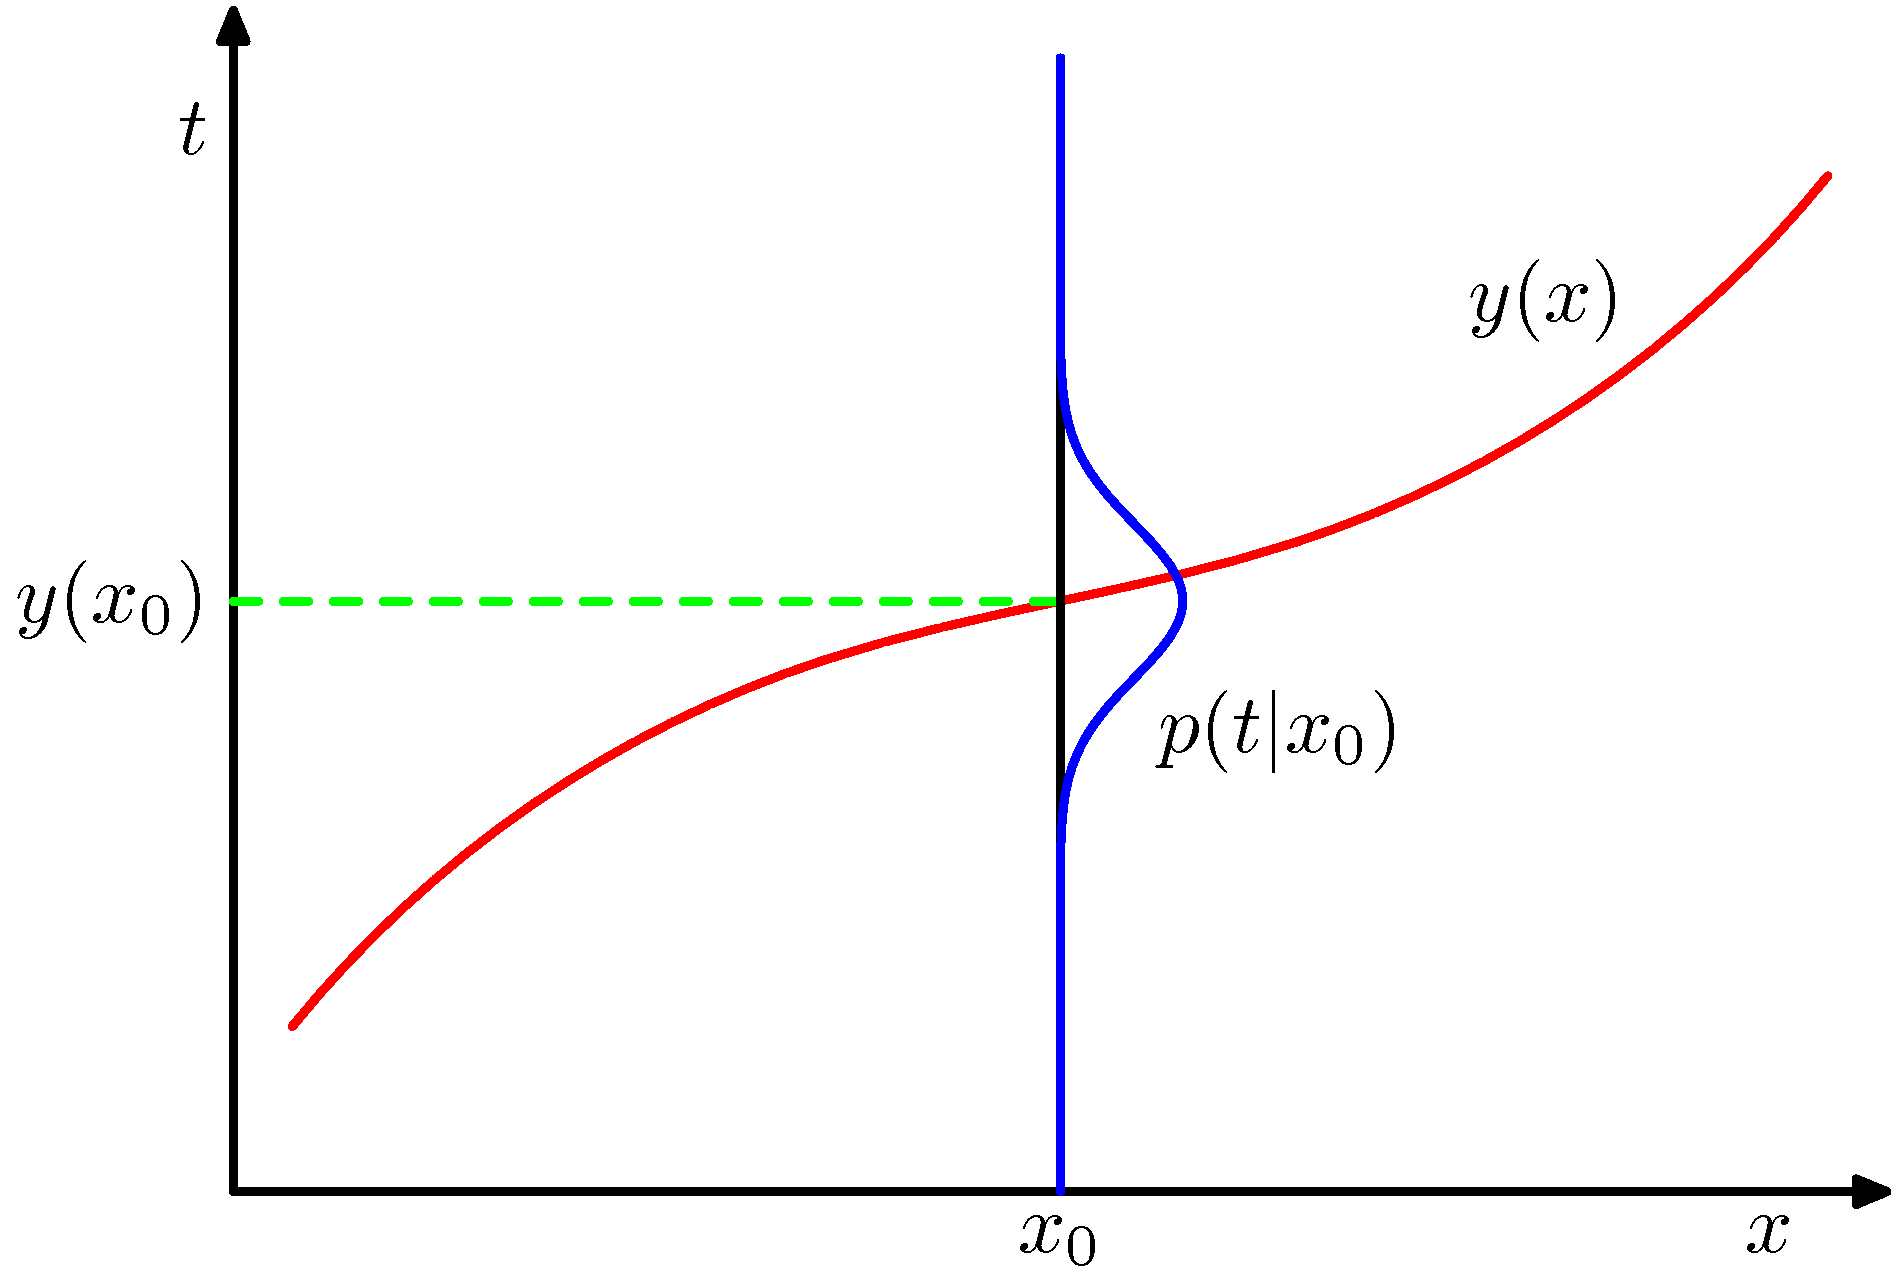
\includegraphics[scale=0.8]{Images/1-28.png}
		\captionsetup{font={small}}
		\caption{使期望平方损失最小化的回归函数y(x),由条件分布$p(t|x)$的均值得到。}
		\label{fig:1-28}
	\end{figure}
	\\
	\indent 我们同样可以利用另一种稍微不太一样的方法推出这个结论,在这个方法中将透露出回归问题的本质。我们已经知道最优解其实就是条件期望,那就可以写出平方项的展开形式:
	\[ \{y(\boldsymbol{\mathrm{x}})-t\}^2 = \{y(\boldsymbol{\mathrm{x}})-\mathbb{E}[t|\boldsymbol{\mathrm{x}}]-t\}^2 = \{y(\boldsymbol{\mathrm{x}})-\mathbb{E}[t|\boldsymbol{\mathrm{x}}]\}^2 + 2\{y(\boldsymbol{\mathrm{x}})-\mathbb{E}[t|\boldsymbol{\mathrm{x}}]\}\{\mathbb{E}[t|\boldsymbol{\mathrm{x}}]-t\}+\{\mathbb{E}[t|\boldsymbol{\mathrm{x}}]-t\}^2 \] 
	其中为了让符号简洁一些,我们用$\mathbb{E}[t|\boldsymbol{\mathrm{x}}]$来表示$\mathbb{E}_t[t|\boldsymbol{\mathrm{x}}]$。将其代入损失函数并对$t$积分,交叉项就消失了,于是就得到如下的损失函数:
	\begin{equation}
		\mathbb{E}[L]=\int \{y(\boldsymbol{\mathrm{x}})-\mathbb{E}[t|\boldsymbol{\mathrm{x}}]\}^2p(\boldsymbol{\mathrm{x}})\ \mathrm{d}\boldsymbol{\mathrm{x}} + \int \mathrm{var}[t|\bx]p(\boldsymbol{\mathrm{x}})\ \mathrm{d}\boldsymbol{\mathrm{x}}
	\end{equation}
	我们希望求取的函数$y(\boldsymbol{\mathrm{x}})$只出现在第一项中,当$y(\boldsymbol{\mathrm{x}})$等于$\mathbb{E}[t|\boldsymbol{\mathrm{x}}]$时将取得最小值,因为这时该项就会消失了。这其实就是我们刚刚证明的那个结果,最优的最小二乘预测就是条件均值。第二项是$t$的分布的方差关于$\boldsymbol{\mathrm{x}}$的平均值。它表示的是目标数据的内部变化,可以当成是噪声来处理。由于它与$y(\boldsymbol{\mathrm{x}})$相互独立,所以表示的是损失函数中不可减小的部分。\\
	\indent 与分类问题类似,我们可以通过确定适当的概率来做最优决策,也可以直接建立决策模型。同样地,我们可以明确地辨认这三种方法。根据复杂程度降序排列,这些方法分别是:\\
	\textbf{(a)}\ 首先确定联合概率密度$p(\boldsymbol{\mathrm{x}},t)$来解决推断问题。然后进行归一化来求取条件概率密度$p(t|\boldsymbol{\mathrm{x}})$,最后用(1.89)来求取条件均值。\\
	\textbf{(b)}\ 首先确定联合概率密度$p(\boldsymbol{\mathrm{x}},t)$来解决推断问题,然后用(1.89)进行边缘化来求取条件均值。\\
	\textbf{(c)}\ 直接根据训练数据求取回归函数$y(\boldsymbol{\mathrm{x}})$。\\
	\indent 这三种方法各自的优势与此前分类问题中的情况类似。\\
	\indent 平方损失并非回归问题中损失函数的唯一选择。实际上,在某些问题中利用平方损失的话可能会导致不怎么好的结果,这就需要采取更复杂一些的方法了。一个比较典型的例子就是在很多反演问题中经常出现条件分布$p(t|\boldsymbol{\mathrm{x}})$具有多个峰值(multimodal)的情况。\color{red} \textbf{——第5.6节} \color{black}在这种情况下我们就会考虑使用一种平方损失的扩展形式,叫做Minkowski损失:
	\begin{equation}
		\mathbb{E}[L_q]=\iint |y(\boldsymbol{\mathrm{x}})-t|^q p(\boldsymbol{\mathrm{x}},t)\ \mathrm{d}\boldsymbol{\mathrm{x}}\ \mathrm{d}t
	\end{equation}
	其中如果$q=2$的话就会退化为期望的平方损失。如图1.29所示是函数$|y-t|^q$关于$y-t$的图像。$\mathbb{E}[L_q]$在$q=2$时的最小值为条件均值,在$q=1$时为条件中位数,在$q \rightarrow 0$时为条件模。\color{red} \textbf{——习题 1.27} \color{black}
	\begin{figure}[ht]
		\begin{minipage}[t]{0.5\linewidth}
		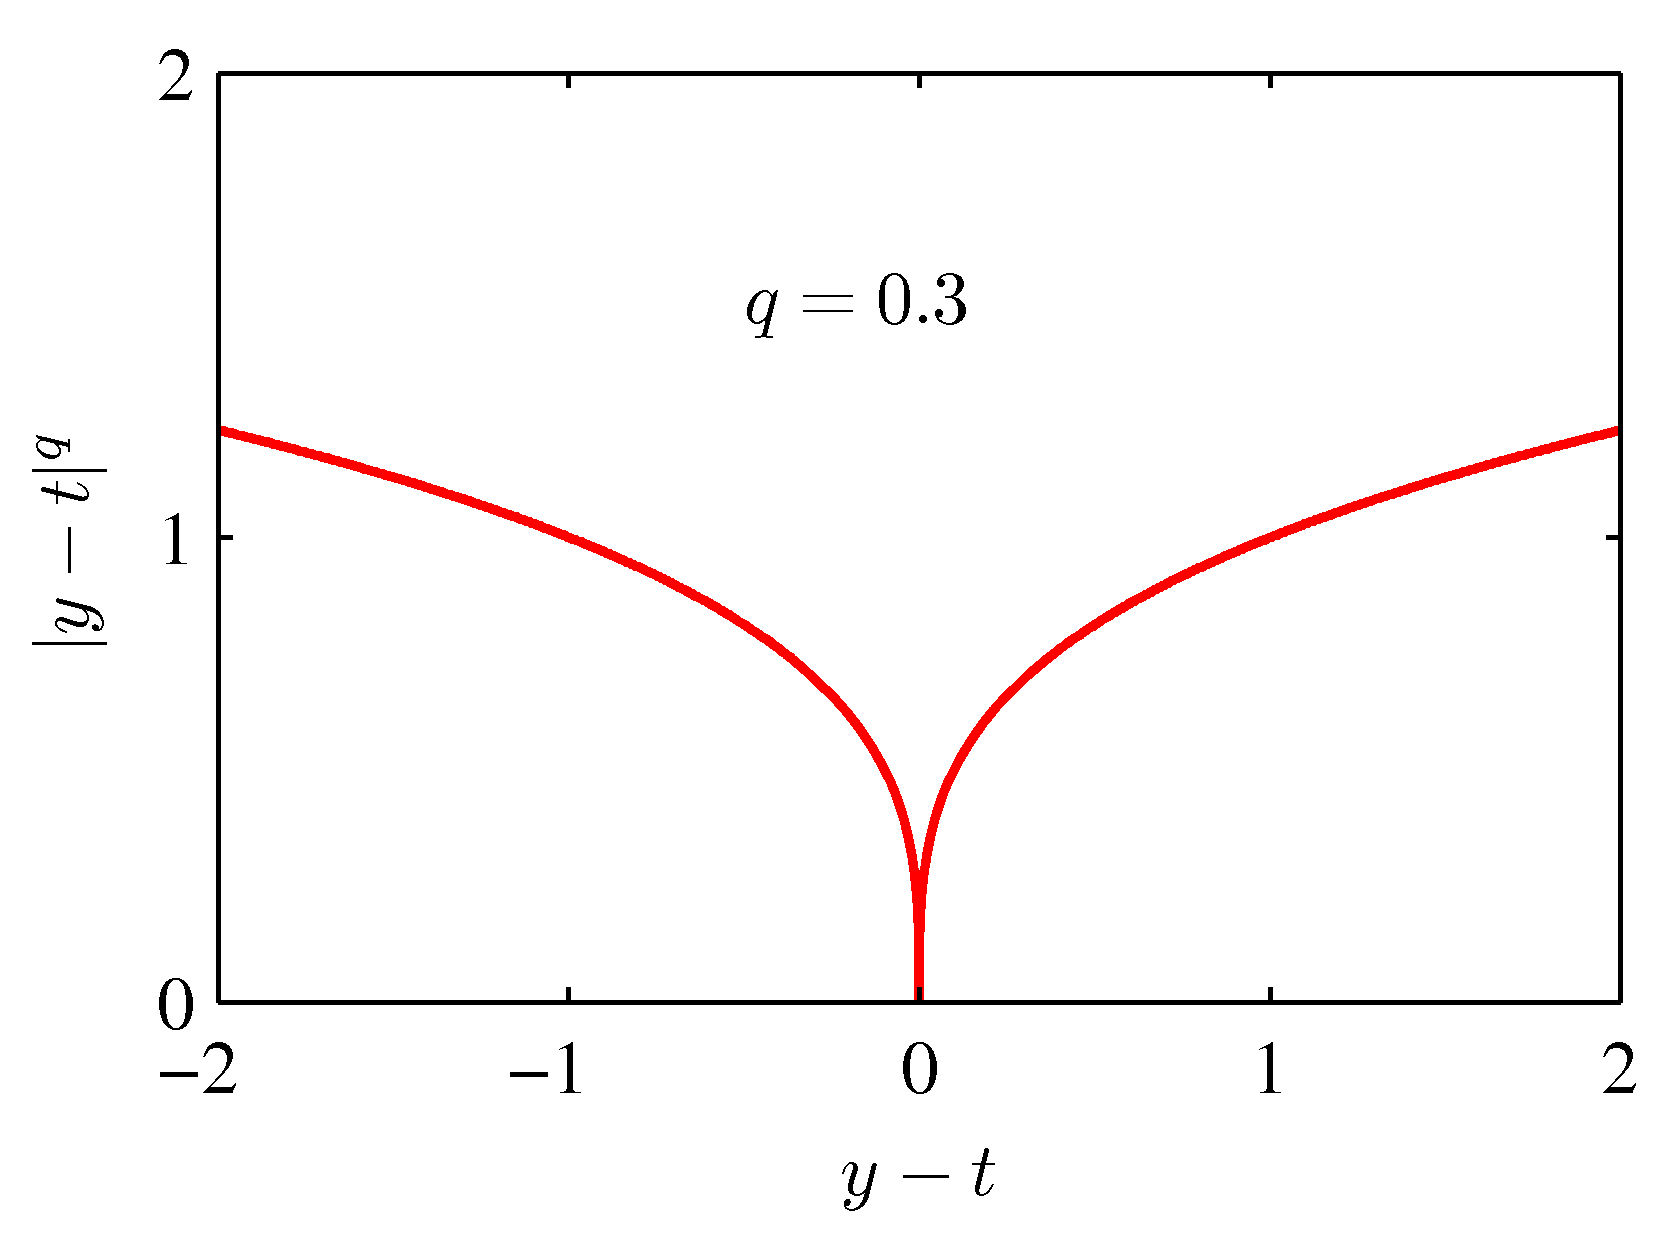
\includegraphics[scale=0.8]{Images/1-29a.png}
		\label{fig:1-29a}
		\end{minipage}
		\begin{minipage}[t]{0.5\linewidth}
		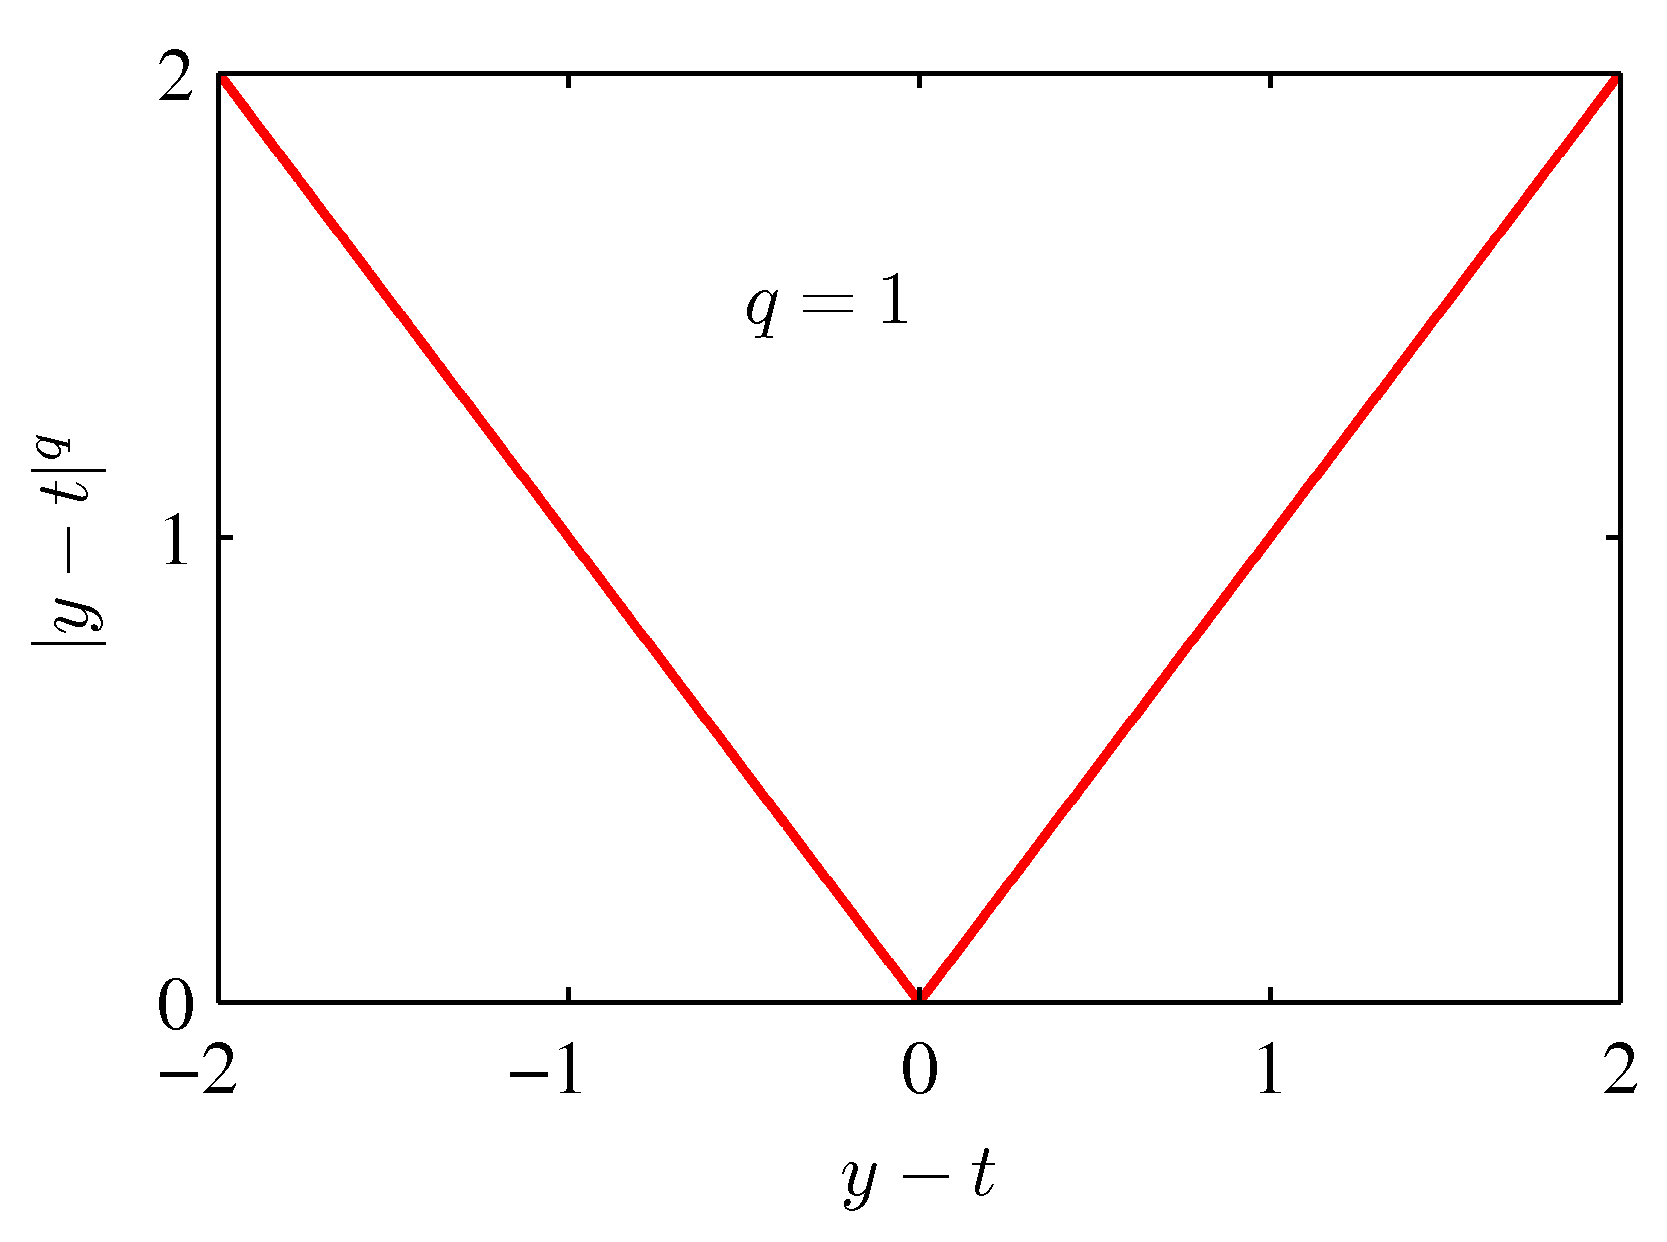
\includegraphics[scale=0.8]{Images/1-29b.png}
		\label{fig:1-29b}\\
		\end{minipage}
		\begin{minipage}[t]{0.5\linewidth}
		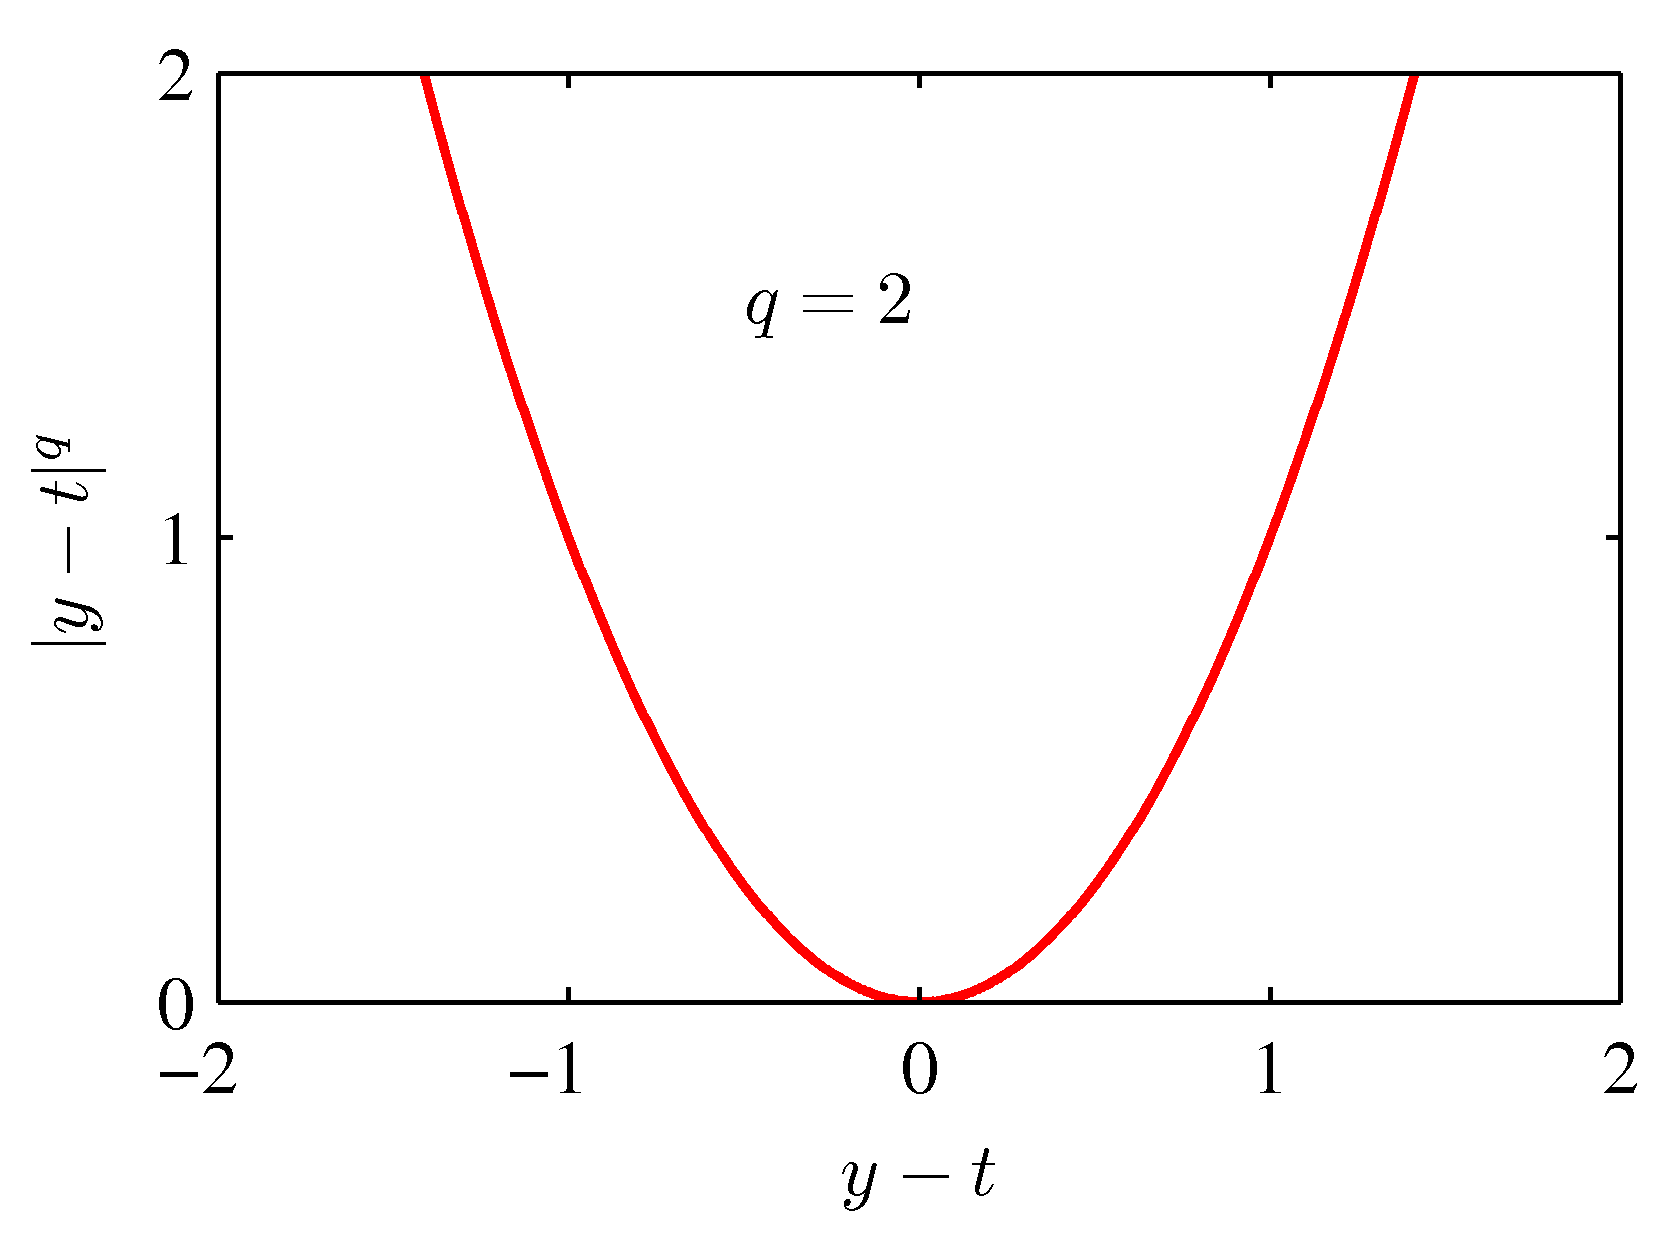
\includegraphics[scale=0.8]{Images/1-29c.png}
		\label{fig:1-29c}
		\end{minipage}
		\begin{minipage}[t]{0.5\linewidth}
		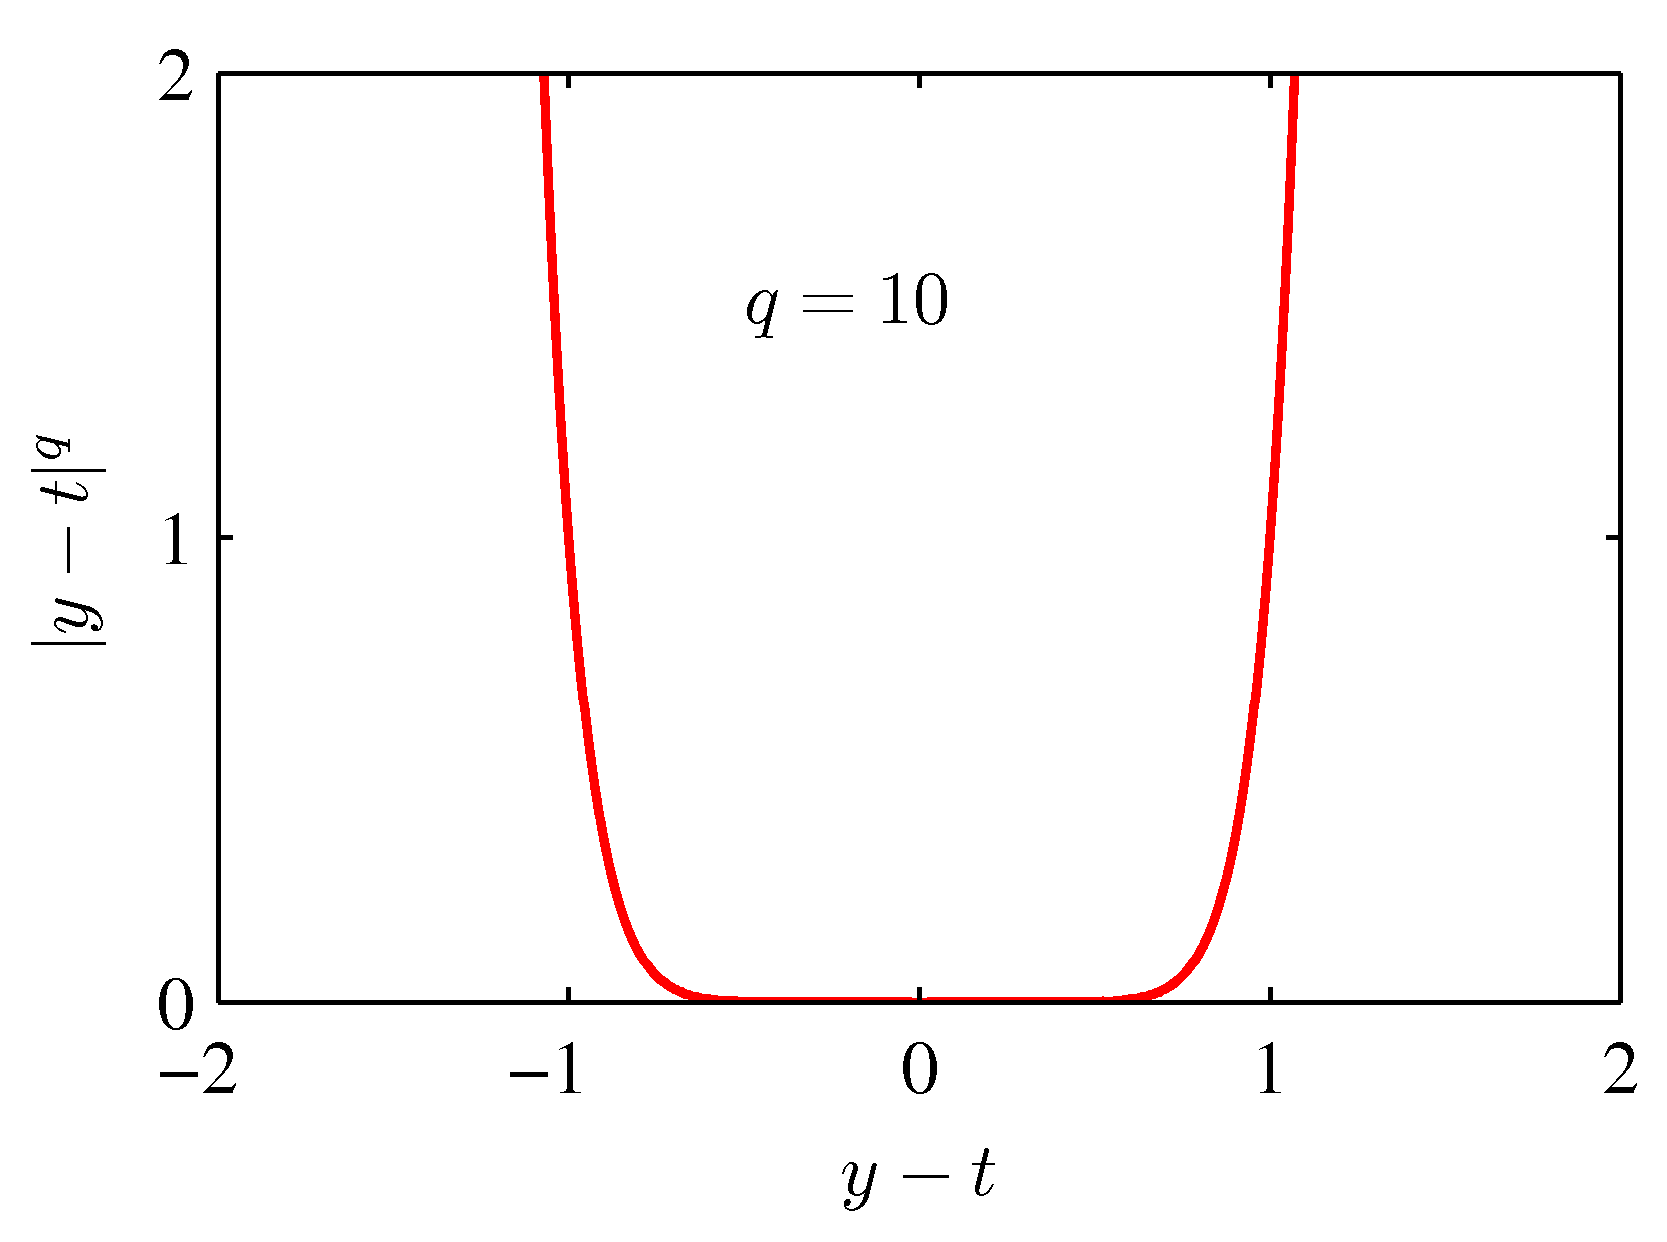
\includegraphics[scale=0.8]{Images/1-29d.png}
		\label{fig:1-29d}
		\end{minipage}
		\captionsetup{font={small}}
		\caption{函数$L_q=|y-t|^q$在$q$取不同值时的图像。}
	\end{figure}
	}
	\section{信息论}
	\noindent{\color{red} \rule[5pt]{\textwidth}{0.1em}}
	\textnormal{
	\indent 在本章中,我们已经讨论了一些概率论和决策论中的概念,这将是本书很多后续内容的基础。我们以信息论领域中一些概念的介绍来结束这个章节,这些概念同样是对模式识别与机器学习技术相当重要的。和前面一样,这里也仅仅介绍一些关键的概念,对于想要获取更多内容的读者,我们建议参考其他的文献(Viterbi and Omura, 1979; Cover and Thomas, 1991; MacKay, 2003)。\\
	\indent 我们从离散随机变量$x$开始,当我们拿到这个变量的某个值后,我们究竟获取到了多少的信息呢?信息的数量可以看成是学习$x$过程中的“惊喜程度”。比方说,要是我们刚听说有人搞了个大新闻,比起小新闻来说,我们在前者中得到的信息量肯定是更大的,要是发生的事情是日常事件,那就得不到什么信息了。对于信息量的衡量是基于概率分布$p(x)$的,于是我们就很想找到一个$p(x)$的单调函数$h(x)$,从而描述信息量。对于两个无关的事件$x$和$y$而言,$h(\cdot)$的形式比较容易确定,因为从这两个事件中得到的信息收益是从二者中分别得到的信息收益的总和,也就是$h(x,y)=h(x)+h(y)$。两个无关的事件一定是统计独立的,于是$p(x,y)=p(x)p(y)$。从这两个关系中,可以比较容易地推出,$h(x)$一定是$p(x)$的对数函数。于是可以得到\color{red} \textbf{——习题 1.28} \color{black}
	\begin{equation}
		h(x)=-\log_2p(x)
	\end{equation}
	其中的负号表示信息量是非负数。需要注意的是,一个低概率的事件$x$对应的是一个很高的信息量。对数的底数是可以随意确定的,现在我们先用信息论中比较普遍使用的以2为底数的对数。我们将会看到,在这种情况下,$h(x)$的单位是位(bits, binary digits)。\\
	\indent 现在我们假设一个信息的发送者要将某个随机变量的值传递给接收者。在传递的过程中,信息量的平均数是对(1.92)求取关于概率分布$p(x)$的期望,也就是
	\begin{equation}
		\mathrm{H}[x]=-\sum_x p(x)\log_2 p(x)
	\end{equation}
	这是一个很重要的值,称为随机变量$x$的熵(entropy)。注意,$\lim_{p \rightarrow 0} p\log_2 p = 0$,所以对于一切使得$p(x)=0$的$x$,我们认为$p(x)\log_2 p(x)=0$。\\
	\indent 到目前为止,我们用比较启发式的方式给出了信息的定义(1.92)和对应的熵的定义(1.93)。现在我们来证明这些定义确实具备实用的属性。假设一个随机变量有8个状态,每一种状态都是等可能的。为了与接收者进行$x$的交流,我们需要传递一个长度为3位的信息。注意,该变量的熵为
		\[ \mathrm{H}[x]=-8 \times \frac{1}{8}\log_2 \frac{1}{8} =3 \ \mathrm{bits} \]
	现在引入一个案例,在这个案例中8个状态$\{a,b,c,d,e,f,g,h\}$分别对应的概率是$(\frac{1}{2},\frac{1}{4},\frac{1}{8},\frac{1}{16},\frac{1}{64},\frac{1}{64},\frac{1}{64},\frac{1}{64})$。这种情况下的熵就变成了:
		\[ \mathrm{H}[x]=-\frac{1}{2}\log_2 \frac{1}{2} - \frac{1}{4}\log_2 \frac{1}{4} - \frac{1}{8}\log_2 \frac{1}{8} - \frac{1}{16}\log_2 \frac{1}{16} -\frac{4}{64}\log_2 \frac{1}{64} = 2\ \mathrm{bits} \]
	可以看出,非均匀分布的熵比均匀分布要小,从混乱程度的角度来解释熵可以让我们对此理解得更加清楚。首先我们来看究竟如何表示变量的状态取值并进行传递。和之前一样,我们可以用一个长度为3位的数字代码来表示。然而由于现在是非均匀分布,我们就可以利用这一特点让总体的代码长度短一些,用较短的代码表示概率较高的事件,但低概率事件的代码会长一些。比如说我们可以用如下代码串表示状态$\{a,b,c,d,e,f,g,h\}$:$0,10,110,1110,111100,111101,111110,111111$。需要传输的代码长度均值为:
	\[ \mathrm{average\ code\ length} = \frac{1}{2} \times 1 + \frac{1}{4} \times 2 + \frac{1}{8} \times 3 + \frac{1}{16} \times 4 + 4 \times \frac{1}{64} \times 6 = 2\ \mathrm{bits}\]
	这和随机变量的熵是相同的。但是这样的短码是不能直接拿来用的,因为可能会导致歧义,比如说,11001110这个代码串,可以解码成$c$,$a$和$d$的组合。\\
	\indent 熵与最短代码长度的关系是有关联的。无噪声编码理论(noiseless coding theorem, Shannon, 1948)表明了熵是随机变量的传递中所需要数字位数的下界。\\
	\indent 从现在开始,我们转向使用自然对数来定义熵,因为这个会为后续的内容提供不少的方便。在这种情况下,熵的单位就变成了“nats”而不是“bits”了,它们的区别仅仅在于参数$\ln 2$而已。\\
	\indent 我们已经以平均信息量的形式定义了熵,这里是需要明确随机变量的不同状态的。其实在物理学中,熵的概念要算得上长者了,它是基于平衡热力学的背景而提出,后来又在统计力学的发展中对混乱程度的衡量给出了更加深刻的解释。我们可以通过一个例子来理解熵在这个角度上的理解。假设有一组完全相同的$N$个物体,这$N$个物体会被划分到一堆箱子里,使得第$i$个箱子里有$n_i$个物体。把物体分配到箱子里的办法有多少种呢?第一个物体有$N$种选择,第二个物体有$(N-1)$种,以此类推,那么将$N$个物体分配到箱子里的办法一共有$N!$种,其中$N!$为阶乘,即$N! = N \times (N-1) \times ... \times 2 \times 1$。然而,我们又不希望对每个箱子中物体的排列顺序加以区分。在第$i$个箱子中,有$n_i!$种排列物体的方式,所以将$N$个物体分配到箱子中的方法总数为
	\begin{equation}
		W=\frac{N!}{\prod_i n_i !}
	\end{equation}
	称为“多样性”(multiplicity)。那么熵就可以定义成带有适当系数的多样性的对数
	\begin{equation}
		\mathrm{H} = \frac{1}{N}\ln W = \frac{1}{N} \ln N! - \frac{1}{N}\sum_i \ln n_i !
	\end{equation}
	现在假设$N \rightarrow \infty$,这样$n_i/N$就趋近于1了,利用斯特林公式(Stirling’s approximation):
	\begin{equation}
		\ln N! \approx N \ln N - N
	\end{equation}
	从而有
	\begin{equation}
		\mathrm{H} = - \lim_{N \rightarrow \infty} \sum_i \left( \frac{n_i}{N} \right) \ln \left( \frac{n_i}{N}\right) = -\sum_i p_i \ln p_i
	\end{equation}
	里面用到了$\sum_i n_i = N$。其中$p_i = \lim_{N \rightarrow \infty} (n_i/N)$是一个物体被分配到第$i$个箱子的概率。在物理学术语中,箱子里的物体具体排列顺序称为微观状态(microstate),而比例$n_i/N$的整体分布称为宏观状态(macrostate)。多样性$W$其实是宏观状态中的权重(weight)。\\
	\indent 我们可以将箱子解释为离散随机变量$X$的状态$x_i$,$p(X=x_i)=p_i$。那么随机变量$X$的熵就是
	\begin{equation}
		\mathrm{H}[p] = - \sum_i p(x_i)\ln p(x_i)
	\end{equation}
	在某些值附近急剧上升的分布$p(x_i)$对应的熵会比较低,而对于大多数值都比较均匀的分布的熵就相对比较高了,如图1.30所示。
	\begin{figure}[ht]
		\begin{minipage}[t]{0.5\linewidth}
		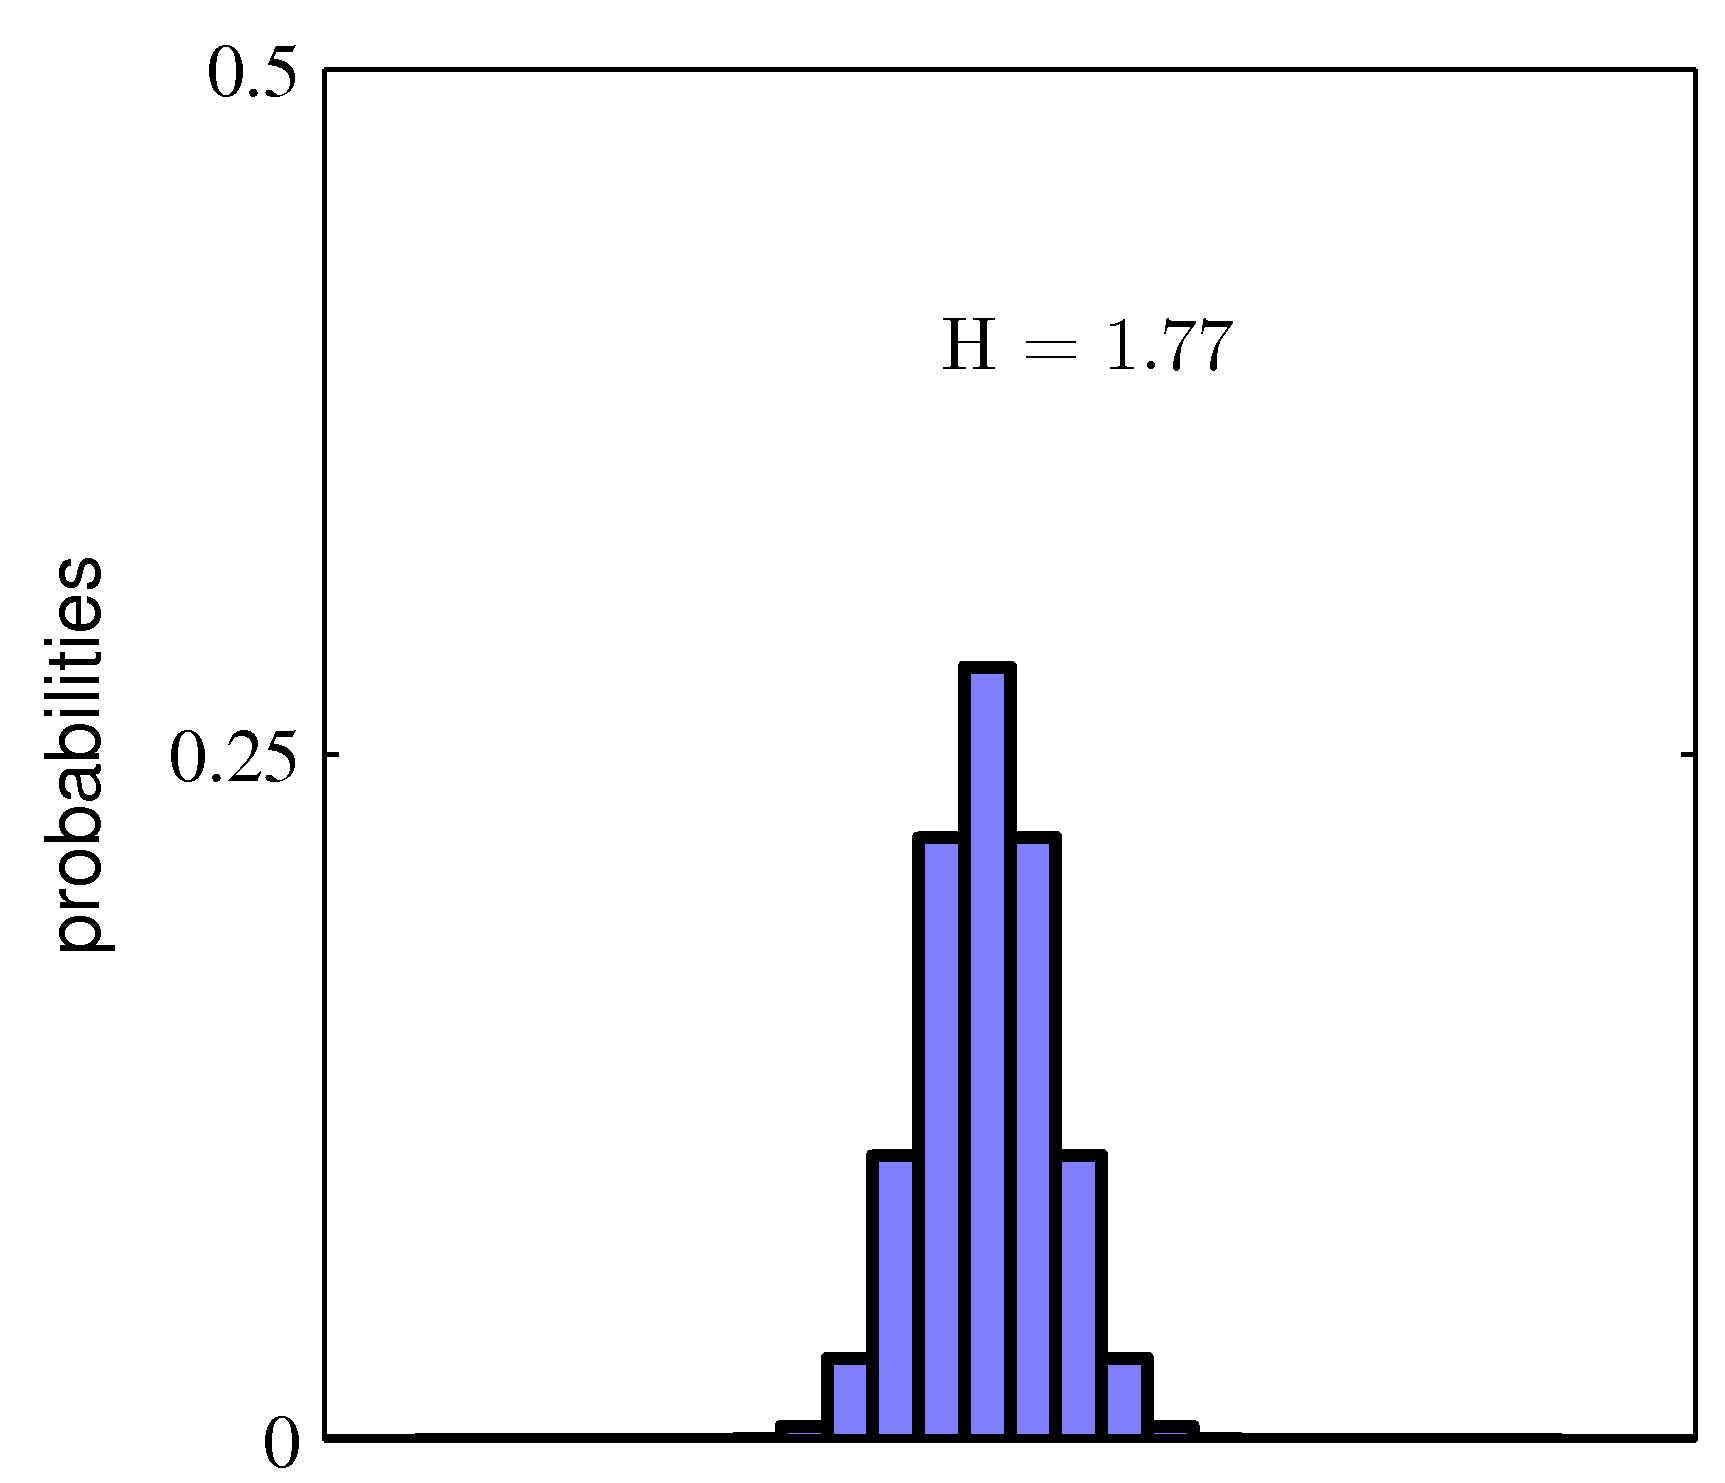
\includegraphics[scale=0.8]{Images/1-30a.png}
		\label{fig:1-30a}
		\end{minipage}
		\begin{minipage}[t]{0.5\linewidth}
		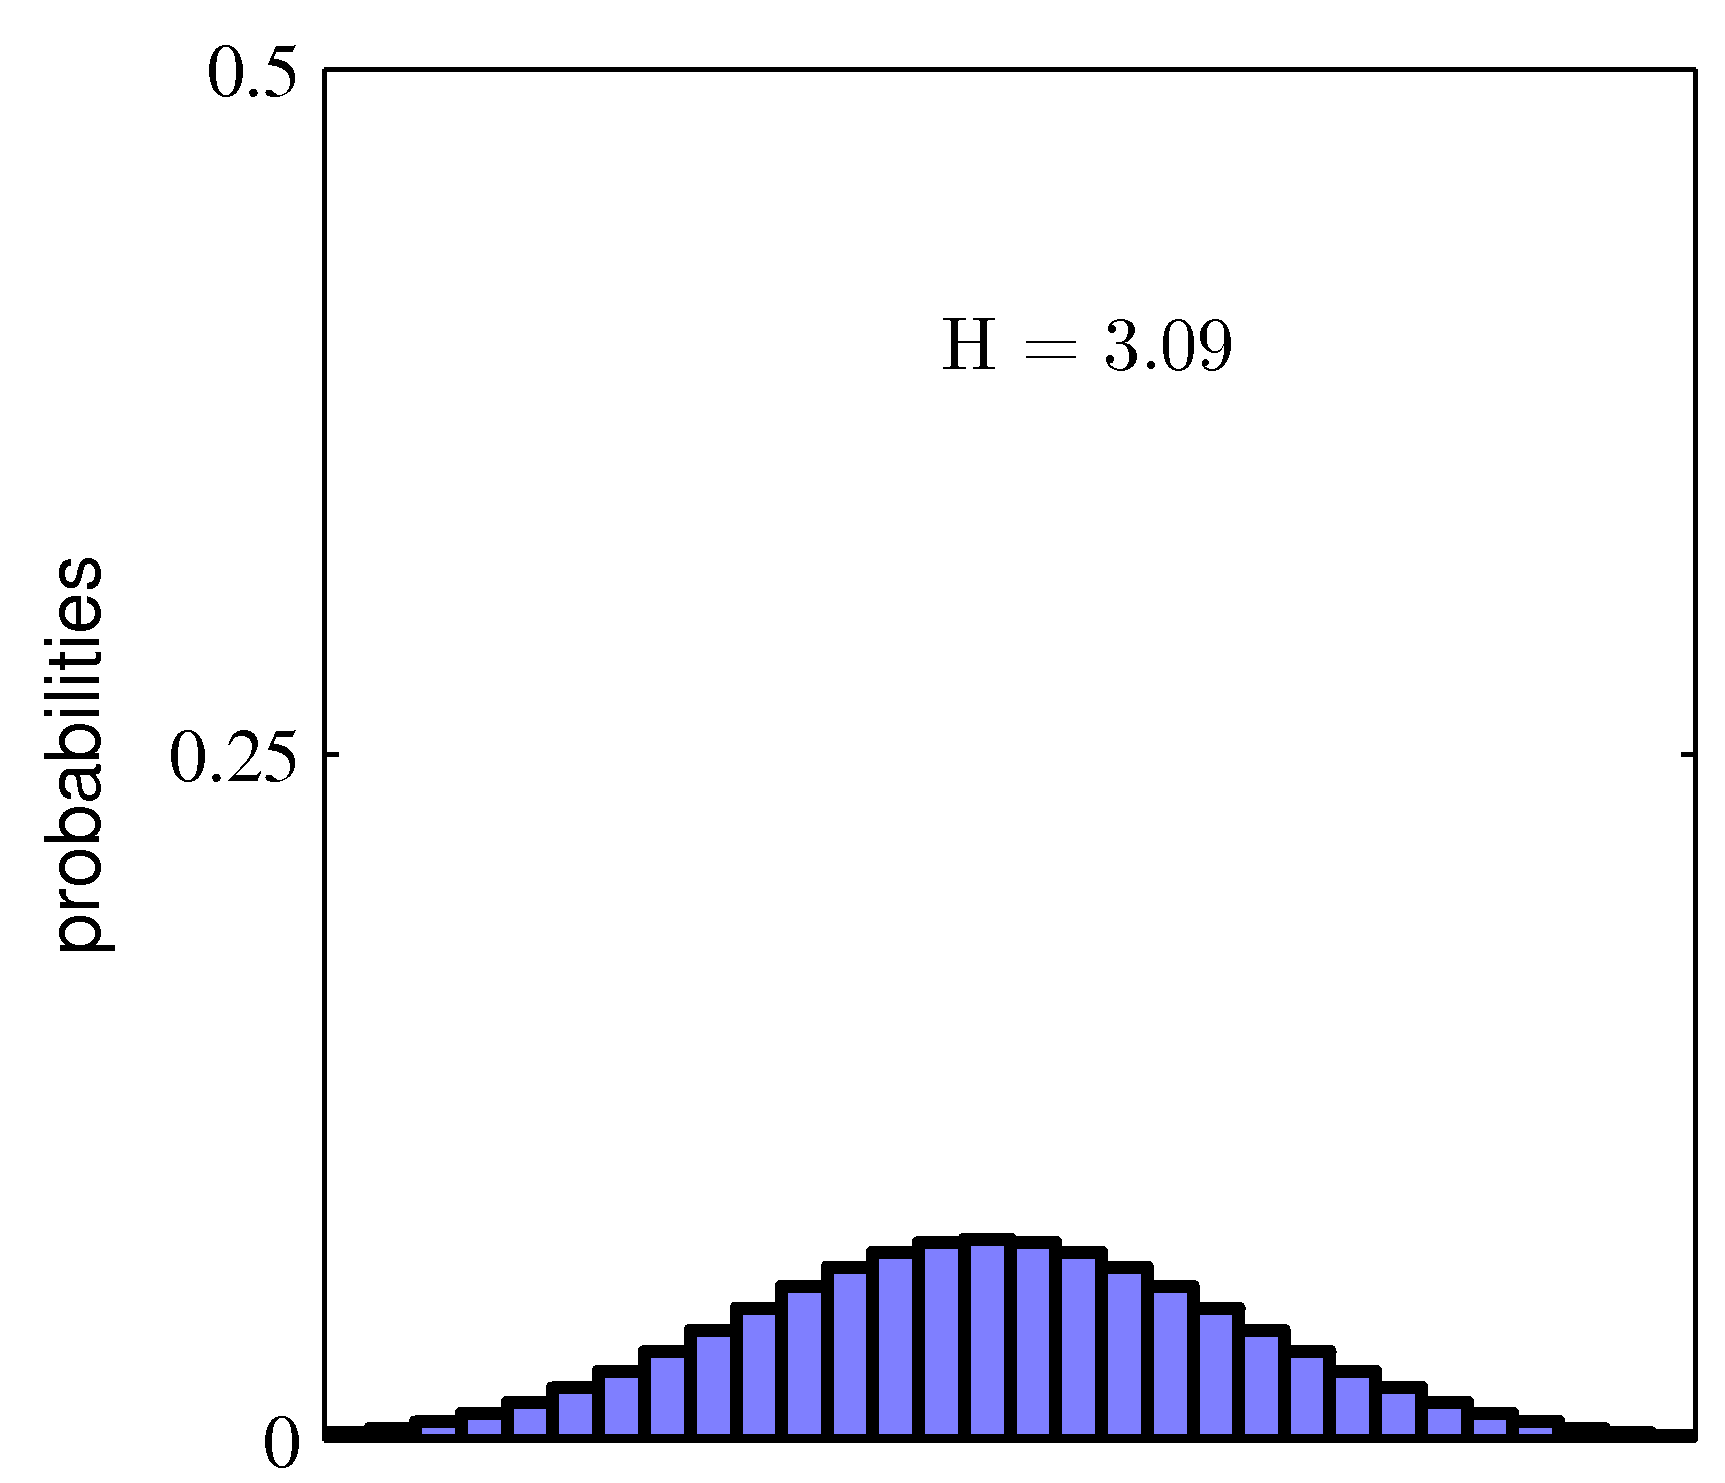
\includegraphics[scale=0.8]{Images/1-30b.png}
		\label{fig:1-30b}
		\end{minipage}
		\captionsetup{font={small}}
		\caption{以30个箱子为例,两个不同概率分布的直方图。表现越平均的分布,熵就越低。在分布为均匀分布时,熵取得最大值$\mathrm{H}=-\ln (1/30) =3.40$。}
	\end{figure}
	\\
	\indent 由于$0 \leqslant p_i \leqslant 1$,所以熵是非负数,而且当且仅当$p_i=0$且一切$p_{j \neq i} =0$时取得最小值0。另一方面可以利用拉格朗日算子进行概率归一化约束,从而对$\mathrm{H}$进行最大化来得到熵的最大值。\color{red} \textbf{——附录E} \color{black}也就是将以下函数:
	\begin{equation}
		\widetilde{\mathrm{H}} = -\sum_i p(x_i) \ln p(x_i) + \lambda \left(\sum_i p(x_i)-1 \right)
	\end{equation}
	进行最大化。我们会发现,在取得最大值时所有的$p(x_i)$都是相等的,而且$p(x_i)=1/M$,$M$为状态$x_i$的总数。对应的熵就是$\mathrm{H} = \ln M$。这个结果也可以通过Jensen不等式来推导出来。\color{red} \textbf{——习题 1.29} \color{black}为了确定驻点处确实是最大值,可以对熵求二阶导数,也就是
	\begin{equation}
		\frac{\partial\mathrm{^2} \widetilde{H}}{\partial p(x_i) \partial p(x_j)} = -I_{ij}\frac{1}{p_i}
	\end{equation}
	其中$I_{ij}$为单位矩阵的元素。\\
	\indent 我们可以将熵的定义扩展为到连续变量$x$的分布上。首先将$x$分配到宽度为$\Delta$的区间中;然后假设$p(x)$是连续的,根据中值定理(mean value theorem, Weisstein, 1999),对于任意区间,一定存在$x_i$,使得
	\begin{equation}
		\int_{i\Delta}^{(i+1)\Delta} p(x)\ \mathrm{d}x = p(x_i) \Delta
	\end{equation}
	现在我们可以通过在$x$落入第$i$个区间时给$x$任意赋值来量化连续变量$x$了。那么观测到$x_i$值的概率就是$p(x_i)\Delta$。这就给出了一个离散形式的计算熵的方式:
	\begin{equation}
		\mathrm{H}_{\Delta}=-\sum_{i}p(x_i)\Delta \ln(p(x_i)\Delta) = -\sum_i p(x_i)\Delta \ln p(x_i)-\ln \Delta
	\end{equation}
	与(1.101)一样,其中$\sum_i p(x_i) \Delta =1$。现在我们直接忽略(1.102)等号右侧的第二项$\ln \Delta$,并取极限$\Delta \rightarrow 0$。(1.102)等号右侧的第一项在取极限时会趋近于$p(x)\ln p(x)$的积分,也就是
	\begin{equation}
		\lim_{\Delta \rightarrow 0} \left\{ - \sum_i p(x_i)\Delta \ln p(x_i) \right\} = -\int p(x)\ln p(x)\ \mathrm{d}x
	\end{equation}
	其中等号右侧的值称为差分熵(differential entropy)。我们可以看出,熵的离散形式和连续形式的区别在于$\ln \Delta$,在$\Delta \rightarrow 0$时会发散。这反映了想要非常精确地直接指定一个连续变量,需要很多位才行。对于多个连续变量的概率密度,用$\boldsymbol{\mathrm{x}}$表示变量组成的向量,则差分熵为
	\begin{equation}
		\mathrm{H}[\boldsymbol{\mathrm{x}}] = -\int p(\boldsymbol{\mathrm{x}}) \ln p(\boldsymbol{\mathrm{x}}) \mathrm{d}\boldsymbol{\mathrm{x}}
	\end{equation}
	\indent 在离散分布中,我们发现最大熵是在变量的分布为均匀分布时取得的。现在我们考虑一下连续分布的情况。为了确定这个情况下熵的最大值,引入对$p(x)$的一阶矩、二阶矩的约束,以及归一化约束是很有必要的。这三个约束分别是
	\begin{align}
		\int_{-\infty}^{\infty} p(x)\ \mathrm{d}x &= 1 \\
		\int_{-\infty}^{\infty} xp(x)\ \mathrm{d}x &= \mu \\
		\int_{-\infty}^{\infty} (x-\mu)^2p(x)\ \mathrm{d}x &= \sigma^2
	\end{align}
	这个约束优化问题可以利用拉格朗日算子来解决。\color{red} \textbf{——附录 E} \color{black}于是我们关于$p(x)$对以下式子求最大值:
	\begin{equation*}
	\begin{split}
		&-\int_{-\infty}^{\infty} p(x)\ln p(x)\ \mathrm{d}x + \lambda_1 \left(\int_{-\infty}^{\infty} p(x)\ \mathrm{d}x -1\right)\\
		&+ \lambda_2 \left(\int_{-\infty}^{\infty} xp(x)\ \mathrm{d}x -\mu \right) +\lambda_3\left(\int_{-\infty}^{\infty} (x-\mu)^2p(x)\ \mathrm{d}x - \sigma^2\right)
	\end{split}
	\end{equation*}
	采用变分法(\color{red} \textbf{附录 D}\color{black}),设该式的导数为0,于是
	\begin{equation}
		p(x)=\exp\left\{-1+\lambda_1+\lambda_2 x + \lambda_3(x-\mu)^2\right\}
	\end{equation}
	拉格朗日算子可以通过将这个结果回代到此前的三个约束等式中,最终的结果为\color{red} \textbf{——习题 1.34} \color{black}
	\begin{equation}
		p(x)=\frac{1}{(2\pi\sigma^2)^{1/2}}\exp\left\{-\frac{(x-\mu)^2}{2\sigma^2}\right\}
	\end{equation}
	所以使得差分熵取得最大值的分布就是高斯分布。需要注意的是,我们没有基于熵必须不小于0来建立约束。然而,最后我们得到的分布确实是非负的,可以看出这个约束是没有必要的。\\
	\indent 如果我们对高斯分布求取差分熵,可以得到\color{red} \textbf{——习题 1.35} \color{black}
	\begin{equation}
		\mathrm{H}[x]=\frac{1}{2}\left\{1+\ln(2\pi\sigma^2)\right\}
	\end{equation}
	于是我们可以再次看出,$\sigma^2$越大,分布就越“宽”,熵就越大。这个结果显示,与离散熵不同,差分熵是可能取负数的,因为(1.110)中的$\mathrm{H}(x)$在$\sigma^2<1/(2\pi e)$时小于0。\\
	\indent 假设我们有一个联合概率分布$p(\boldsymbol{\mathrm{x}},\boldsymbol{\mathrm{y}})$,其中$\boldsymbol{\mathrm{x}}$和$\boldsymbol{\mathrm{y}}$是成对的。如果一个$\boldsymbol{\mathrm{x}}$已知,那么确定$\boldsymbol{\mathrm{y}}$需要的附加信息是$-\ln p(\boldsymbol{\mathrm{y}}|\boldsymbol{\mathrm{x}})$。于是确定$\boldsymbol{\mathrm{y}}$需要的平均附加信息可以写成:
	\begin{equation}
		\mathrm{H}[\boldsymbol{\mathrm{y}}|\boldsymbol{\mathrm{x}}]=-\iint p(\boldsymbol{\mathrm{y}},\boldsymbol{\mathrm{x}})\ln p(\boldsymbol{\mathrm{y}}|\boldsymbol{\mathrm{x}})\ \mathrm{d}\boldsymbol{\mathrm{y}}\ \mathrm{d}\boldsymbol{\mathrm{x}}
	\end{equation}
	上式称为给定$\boldsymbol{\mathrm{x}}$的条件下$\boldsymbol{\mathrm{y}}$的条件熵(conditional entropy)。可以比较容易地看出,利用乘法规则,条件熵满足\color{red} \textbf{——习题 1.37} \color{black}
	\begin{equation}
		\mathrm{H}[\boldsymbol{\mathrm{x}},\boldsymbol{\mathrm{y}}] = \mathrm{H}[\boldsymbol{\mathrm{y}}|\boldsymbol{\mathrm{x}}] + \mathrm{H}[\boldsymbol{\mathrm{x}}]
	\end{equation}
	其中$\mathrm{H}[\boldsymbol{\mathrm{x}},\boldsymbol{\mathrm{y}}]$为$p(\boldsymbol{\mathrm{x}},\boldsymbol{\mathrm{y}})$的差分熵,$\mathrm{H}[\boldsymbol{\mathrm{x}}]$为边缘概率分布$p(\boldsymbol{\mathrm{x}})$的差分熵。于是用于描述$\boldsymbol{\mathrm{x}}$和$\boldsymbol{\mathrm{y}}$的信息可以由描述$\boldsymbol{\mathrm{x}}$所需的信息加上给定$\boldsymbol{\mathrm{x}}$的情况下确定$\boldsymbol{\mathrm{y}}$所需的附加信息来得到。}
	\subsection{相对熵与互信息}
	\textnormal{在本节此前的内容中,我们已经介绍了信息论的一些相关概念,包括最重要的关于熵的定义和分析。现在我们开始将这些内容应用于模式识别。假设我们现在有一个未知的分布$p(\boldsymbol{\mathrm{x}})$,并利用一个近似的分布$q(\boldsymbol{\mathrm{x}})$对它进行建模。如果我们利用$q(\boldsymbol{\mathrm{x}})$来对此前提出的$\boldsymbol{\mathrm{x}}$值的传递构建编码方案,那么根据$q(\boldsymbol{\mathrm{x}})$而非真实分布$p(\boldsymbol{\mathrm{x}})$给定的$\boldsymbol{\mathrm{x}}$的值(假设我们选择了很高效的编码方案)的情况下,信息的平均附加量(以nats为单位)可以根据以下公式计算:
	\begin{equation}
		\begin{split}
			\mathrm{KL}(p||q) &= -\int p(\boldsymbol{\mathrm{x}})\ln q(\boldsymbol{\mathrm{x}}) - \left(-\int p(\boldsymbol{\mathrm{x}})\ln q(\boldsymbol{\mathrm{x}})\ \mathrm{d}\boldsymbol{\mathrm{x}}\right) \\
			&= -\int p(\boldsymbol{\mathrm{x}}) \ln \left\{\frac{q(\boldsymbol{\mathrm{x}})}{p(\boldsymbol{\mathrm{x}})}\ \mathrm{d}\boldsymbol{\mathrm{x}} \right\}
		\end{split}
	\end{equation}
	这就是分布$p(\boldsymbol{\mathrm{x}})$和$q(\boldsymbol{\mathrm{x}})$之间的相对熵(relative entropy)或者称为Kullback-Leibler距离,亦或称为KL差(Kullback and Leibler, 1951)。需要注意的是,这个公式并不具备对称性,也就是说$\mathrm{KL}(p||q) \neq \mathrm{KL}(q||p)$。\\
	\indent 现在我们来证明Kullback-Leibler距离满足$\mathrm{KL}(p||q) \geqslant 0$,当且仅当$p(\boldsymbol{\mathrm{x}})=q(\boldsymbol{\mathrm{x}})$时等号成立。为了证明这个问题,我们首先介绍凸函数(convex function)的概念。如果函数$f(x)$的任意一条弦要么位于函数上,要么位于函数的上方,那么函数$f(x)$就是凸函数,如图1.31所示。
	\begin{figure}[ht]
		\centering
		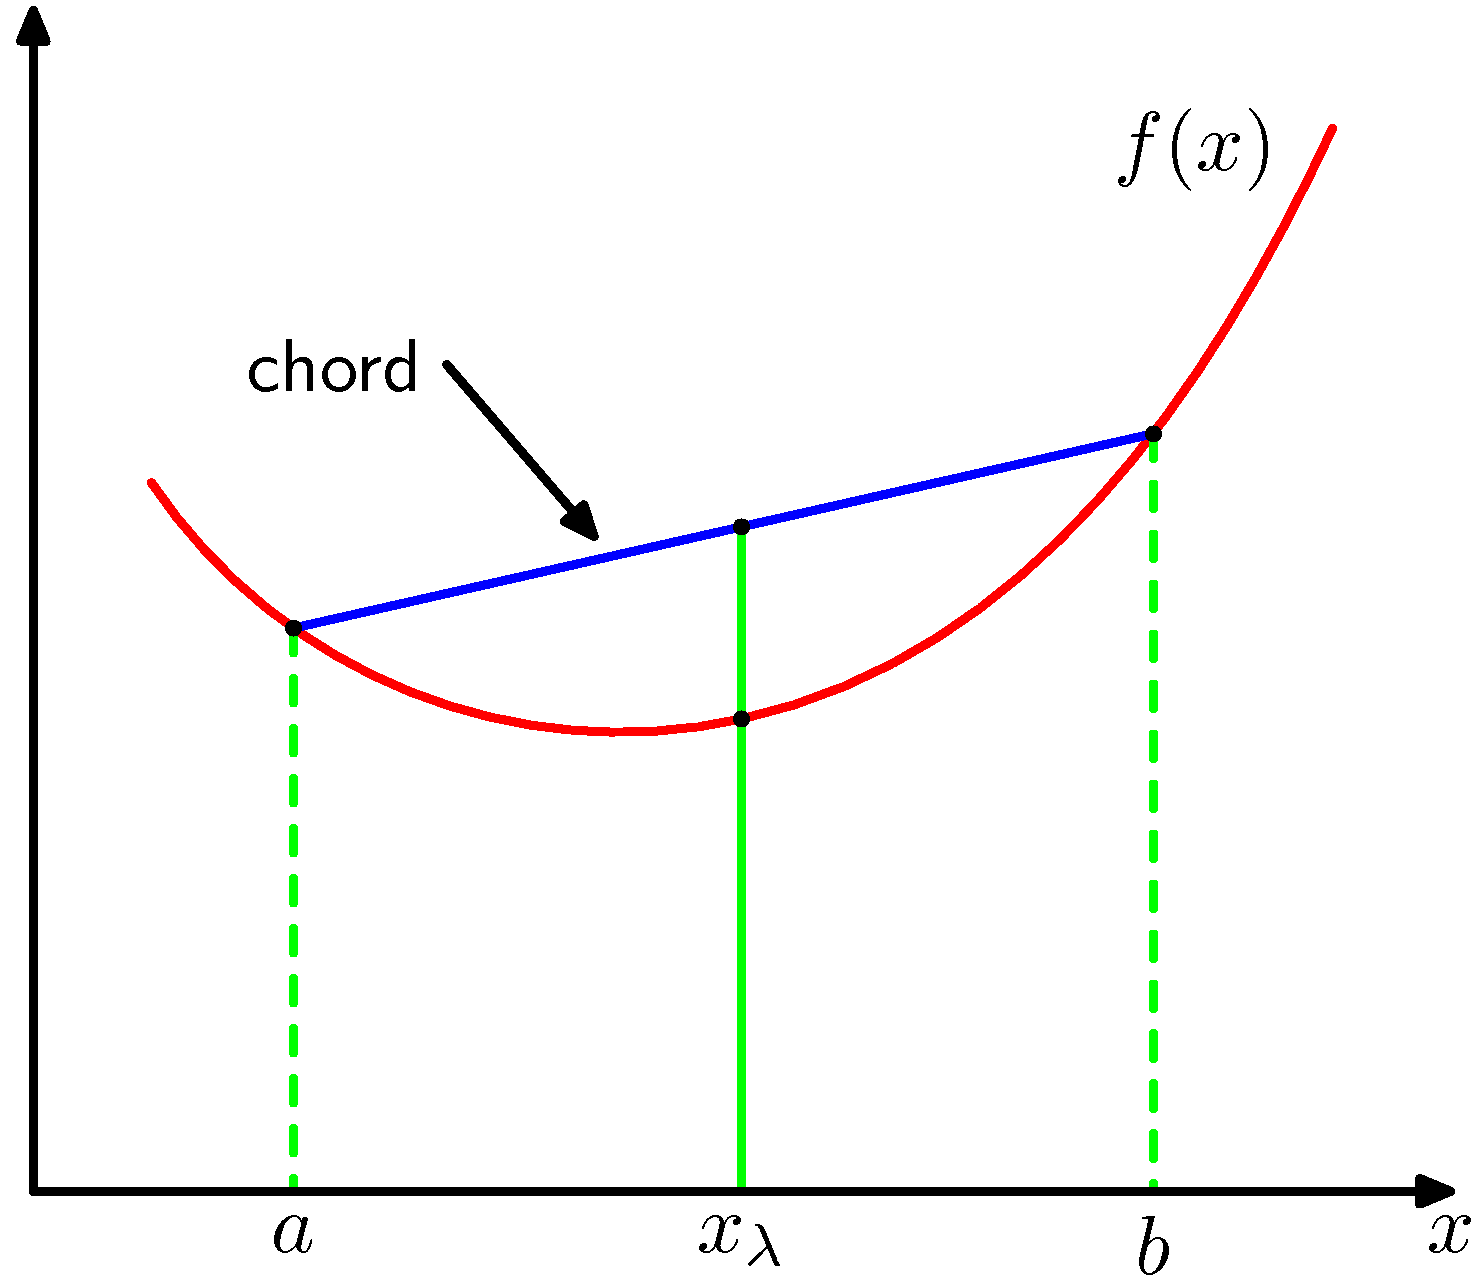
\includegraphics[scale=0.8]{Images/1-31.png}
		\captionsetup{font={small}}
		\caption{凸函数$f(x)$。它的每条弦(蓝色直线)都在自身(红色曲线)上或者自身的上方。}
		\label{fig:1-31}
	\end{figure}
	\\
	\indent 对于$x=a$和$x=b$区间内所有的$x$都可以写成$\lambda a + (1-\lambda) b$的形式,其中$0 \leqslant \lambda \leqslant 1$,在弦上对应的点是$\lambda f(a) + (1-\lambda) f(b)$,对应的函数值为$f(\lambda a + (1-\lambda)b)$。于是有一条性质:
	\begin{equation}
		f(\lambda a + (1-\lambda)b) \leqslant \lambda f(a) + (1-\lambda)f(b)
	\end{equation}
	这个性质与函数的二阶导数处处为正是等价的。\color{red} \textbf{——习题 1.36} \color{black}凸函数的典型例子是$x\ln x (x>0)$和$x^2$。如果上式中的等号仅在$\lambda=0$和$\lambda=1$时成立,那么$f(x)$就是严格凸函数(strictly convex function)。如果一个函数有与此相反的性质,也就是说每一条弦都位于函数上或函数下方,那么就称为凹函数(concave function),对应的还有严格凹函数(strictly concave function)。如果$f(x)$为凸函数,那么$-f(x)$一定为凹函数。\\
	\indent 利用归纳法,根据(1.114)可以证明凸函数$f(x)$满足:\color{red} \textbf{——习题 1.38} \color{black}
	\begin{equation}
		f\left(\sum_{i=1}^M \lambda_i x_i\right) \leqslant \sum_{i=1}^M \lambda_i f(x_i)
	\end{equation}
	\indent 对于任意的$\{x_i\}$集合,$\lambda_i \geqslant 0$ 且$\sum_i \lambda_i =1$。公式(1.115)就是Jensen不等式。如果我们将$\lambda_i$看成是取值为$\{x_i\}$的离散随机变量$x$的概率分布,那么(1.115)就可以写成
	\begin{equation}
		f(\mathbb{E}[x])\leqslant \mathbb{E}[f(x)]
	\end{equation}
	其中$\mathbb{E}(\cdot)$表示期望。对于连续变量,Jensen不等式的形式为
	\begin{equation}
		f\left(\int \boldsymbol{\mathrm{x}}p(\boldsymbol{\mathrm{x}})\ \mathrm{d}\boldsymbol{\mathrm{x}}\right) \leqslant \int f(\boldsymbol{\mathrm{x}})p(\boldsymbol{\mathrm{x}})\ \mathrm{d}\boldsymbol{\mathrm{x}}
	\end{equation}
	\indent 我们可以将(1.117)中的Jensen不等式带入到(1.113)中的Kullback-Leibler距离中,于是有
	\begin{equation}
		\mathrm{KL}(p||q) = - \int p(\boldsymbol{\mathrm{x}}) \ln \left\{\frac{q(\boldsymbol{\mathrm{x}})}{p(\boldsymbol{\mathrm{x}})}\right\}\ \mathrm{d}\boldsymbol{\mathrm{x}} \geqslant - \ln \int q(\boldsymbol{\mathrm{x}})\ \mathrm{d}\boldsymbol{\mathrm{x}} = 0
	\end{equation}
	其中用到了一些结论——$\ln x$是一个凸函数,以及归一化条件$\int q(\boldsymbol{\mathrm{x}})\ \mathrm{d}\boldsymbol{\mathrm{x}} = 1$。实际上,$-\ln x$是一个严格凸函数,所以对于一切$\boldsymbol{\mathrm{x}}$当且仅当$q(\boldsymbol{\mathrm{x}})=p(\boldsymbol{\mathrm{x}})$时等号成立。于是我们就可以将Kullback-Leibler距离看成是两个分布$p(\boldsymbol{\mathrm{x}})$和$q(\boldsymbol{\mathrm{x}})$之间的不相似程度的衡量。\\
	\indent 我们看到,数据的压缩与密度估计(即对未知概率分布进行建模的问题)之间存在密切的联系。因为当我们知道真实的分布之后,就可以对数据进行最有效的压缩。如果我们用了一个与真实分布不同的分布,那么编码一定是会变得低效一些的。而且就常规情况而言,必须要加入到传输之中的附加信息(至少)等于两个分布之间的Kullback-Leibler距离。\\
	\indent 假设数据是从我们希望建模的未知分布$p(\boldsymbol{\mathrm{x}})$生成的。我们可以利用带有可调整参数$\boldsymbol{\mathrm{\theta}}$的参数分布$q(\boldsymbol{\mathrm{x}}|\boldsymbol{\mathrm{\theta}})$来接近这个分布,比如说多元高斯分布。确定参数$\boldsymbol{\mathrm{\theta}}$的方法之一就是关于$\boldsymbol{\mathrm{\theta}}$求取$p(\boldsymbol{\mathrm{x}})$与$p(\boldsymbol{\mathrm{x}}|\boldsymbol{\mathrm{\theta}})$之间Kullback-Leibler距离的最小值。但我们不能直接用这个方法,因为$p(\boldsymbol{\mathrm{x}})$是未知的。不过,假设我们有一个从$p(\boldsymbol{\mathrm{x}})$中取出的有限训练集$\boldsymbol{\mathrm{x}}_n, n=1,...,N$,那么关于$p(\boldsymbol{\mathrm{x}})$的期望就可以用这些数据的有限和,根据(1.35)来逼近。于是
	\begin{equation}
		\mathrm{KL}(p||q)\approx \frac{1}{N}\sum_{n=1}^{N}{-\ln q(\boldsymbol{\mathrm{x}}_n|\boldsymbol{\mathrm{\theta}})+\ln p(\boldsymbol{\mathrm{x}}_n)}
	\end{equation}
	(1.119)中等号右侧的第二项是与$\boldsymbol{\mathrm{\theta}}$相互独立的,第一项是根据训练集估计得到的$\boldsymbol{\mathrm{\theta}}$的分布$q(\boldsymbol{\mathrm{x}}|\boldsymbol{\mathrm{\theta}})$的负对数似然函数。于是我们可以看出,将Kullback-Leibler距离进行最小化,等价于将似然函数进行最大化。\\
	\indent 下面考虑两个变量集合的联合分布$p(\boldsymbol{\mathrm{x}},\boldsymbol{\mathrm{y}})$。如果两个变量集合是相互独立的,那么它们的联合分布就可以拆分成各自边缘分布的乘积$p(\boldsymbol{\mathrm{x}},\boldsymbol{\mathrm{y}})=p(\boldsymbol{\mathrm{x}})p(\boldsymbol{\mathrm{y}})$。如果它们不是相互独立的,我们可以通过研究联合分布与边缘分布乘积之间的Kullback-Leibler距离来衡量这两组变量有多么“接近”相互独立,根据以下公式计算:
	\begin{equation}
		\begin{split}
			\mathrm{I}[\boldsymbol{\mathrm{x}},\boldsymbol{\mathrm{y}}] &\equiv \mathrm{KL}(p(\boldsymbol{\mathrm{x}},\boldsymbol{\mathrm{y}})p(\boldsymbol{\mathrm{x}})p(\boldsymbol{\mathrm{y}}))\\
			&=-\iint p(\boldsymbol{\mathrm{x}},\boldsymbol{\mathrm{y}}) \ln \left(\frac{p(\boldsymbol{\mathrm{x}})p(\boldsymbol{\mathrm{y}})}{p(\boldsymbol{\mathrm{x}},\boldsymbol{\mathrm{y}})}\right)\ \mathrm{d}\boldsymbol{\mathrm{x}}\ \mathrm{d}\boldsymbol{\mathrm{y}}
		\end{split}
	\end{equation}
	该结果称为变量$\boldsymbol{\mathrm{x}}$与$\boldsymbol{\mathrm{y}}$之间的互信息(nutual information)。根据Kullback-Leibler距离的性质,可以看出$\mathrm{I}(\boldsymbol{\mathrm{x}},\boldsymbol{\mathrm{y}}) \geqslant 0$,当且仅当$\boldsymbol{\mathrm{x}}$与$\boldsymbol{\mathrm{y}}$相互独立时等号成立。利用概率的加法规则和乘法规则,可以看出互信息与条件熵是相关的:\color{red} \textbf{——习题 1.41} \color{black}
	\begin{equation}
		\mathrm{I}[\boldsymbol{\mathrm{x}},\boldsymbol{\mathrm{y}}]=\mathrm{H}[\boldsymbol{\mathrm{x}}]-\mathrm{H}[\boldsymbol{\mathrm{x}}|\boldsymbol{\mathrm{y}}]=\mathrm{H}[\boldsymbol{\mathrm{y}}]-\mathrm{H}[\boldsymbol{\mathrm{y}}|\boldsymbol{\mathrm{x}}]
	\end{equation}
	于是可以将互信息看成是给出$\boldsymbol{\mathrm{y}}$的情况下减少的$\boldsymbol{\mathrm{x}}$的不确定性(反之亦然)。从贝叶斯学派的角度来看,我们可以将$p(\boldsymbol{\mathrm{x}})$看成是$\boldsymbol{\mathrm{x}}$的先验分布,$p(\boldsymbol{\mathrm{x}}|\boldsymbol{\mathrm{y}})$为取得新的数据$\boldsymbol{\mathrm{y}}$之后的后验概率。那么互信息自然表示由于新的$\boldsymbol{\mathrm{y}}$的出现,$\boldsymbol{\mathrm{x}}$的不确定性减少的程度了。
	}
\end{document}